\documentclass[twoside]{book}

% Packages required by doxygen
\usepackage{fixltx2e}
\usepackage{calc}
\usepackage{doxygen}
\usepackage[export]{adjustbox} % also loads graphicx
\usepackage{graphicx}
\usepackage[utf8]{inputenc}
\usepackage{makeidx}
\usepackage{multicol}
\usepackage{multirow}
\PassOptionsToPackage{warn}{textcomp}
\usepackage{textcomp}
\usepackage[nointegrals]{wasysym}
\usepackage[table]{xcolor}

% Font selection
\usepackage[T1]{fontenc}
\usepackage[scaled=.90]{helvet}
\usepackage{courier}
\usepackage{amssymb}
\usepackage{sectsty}
\renewcommand{\familydefault}{\sfdefault}
\allsectionsfont{%
  \fontseries{bc}\selectfont%
  \color{darkgray}%
}
\renewcommand{\DoxyLabelFont}{%
  \fontseries{bc}\selectfont%
  \color{darkgray}%
}
\newcommand{\+}{\discretionary{\mbox{\scriptsize$\hookleftarrow$}}{}{}}

% Page & text layout
\usepackage{geometry}
\geometry{%
  a4paper,%
  top=2.5cm,%
  bottom=2.5cm,%
  left=2.5cm,%
  right=2.5cm%
}
\tolerance=750
\hfuzz=15pt
\hbadness=750
\setlength{\emergencystretch}{15pt}
\setlength{\parindent}{0cm}
\setlength{\parskip}{3ex plus 2ex minus 2ex}
\makeatletter
\renewcommand{\paragraph}{%
  \@startsection{paragraph}{4}{0ex}{-1.0ex}{1.0ex}{%
    \normalfont\normalsize\bfseries\SS@parafont%
  }%
}
\renewcommand{\subparagraph}{%
  \@startsection{subparagraph}{5}{0ex}{-1.0ex}{1.0ex}{%
    \normalfont\normalsize\bfseries\SS@subparafont%
  }%
}
\makeatother

% Headers & footers
\usepackage{fancyhdr}
\pagestyle{fancyplain}
\fancyhead[LE]{\fancyplain{}{\bfseries\thepage}}
\fancyhead[CE]{\fancyplain{}{}}
\fancyhead[RE]{\fancyplain{}{\bfseries\leftmark}}
\fancyhead[LO]{\fancyplain{}{\bfseries\rightmark}}
\fancyhead[CO]{\fancyplain{}{}}
\fancyhead[RO]{\fancyplain{}{\bfseries\thepage}}
\fancyfoot[LE]{\fancyplain{}{}}
\fancyfoot[CE]{\fancyplain{}{}}
\fancyfoot[RE]{\fancyplain{}{\bfseries\scriptsize Generated by Doxygen }}
\fancyfoot[LO]{\fancyplain{}{\bfseries\scriptsize Generated by Doxygen }}
\fancyfoot[CO]{\fancyplain{}{}}
\fancyfoot[RO]{\fancyplain{}{}}
\renewcommand{\footrulewidth}{0.4pt}
\renewcommand{\chaptermark}[1]{%
  \markboth{#1}{}%
}
\renewcommand{\sectionmark}[1]{%
  \markright{\thesection\ #1}%
}

% Indices & bibliography
\usepackage{natbib}
\usepackage[titles]{tocloft}
\setcounter{tocdepth}{3}
\setcounter{secnumdepth}{5}
\makeindex

% Hyperlinks (required, but should be loaded last)
\usepackage{ifpdf}
\ifpdf
  \usepackage[pdftex,pagebackref=true]{hyperref}
\else
  \usepackage[ps2pdf,pagebackref=true]{hyperref}
\fi
\hypersetup{%
  colorlinks=true,%
  linkcolor=blue,%
  citecolor=blue,%
  unicode%
}

% Custom commands
\newcommand{\clearemptydoublepage}{%
  \newpage{\pagestyle{empty}\cleardoublepage}%
}

\usepackage{caption}
\captionsetup{labelsep=space,justification=centering,font={bf},singlelinecheck=off,skip=4pt,position=top}

%===== C O N T E N T S =====

\begin{document}

% Titlepage & ToC
\hypersetup{pageanchor=false,
             bookmarksnumbered=true,
             pdfencoding=unicode
            }
\pagenumbering{alph}
\begin{titlepage}
\vspace*{7cm}
\begin{center}%
{\Large Cool\+A\+PI }\\
\vspace*{1cm}
{\large Generated by Doxygen 1.8.14}\\
\end{center}
\end{titlepage}
\clearemptydoublepage
\pagenumbering{roman}
\tableofcontents
\clearemptydoublepage
\pagenumbering{arabic}
\hypersetup{pageanchor=true}

%--- Begin generated contents ---
\chapter{Hierarchical Index}
\section{Class Hierarchy}
This inheritance list is sorted roughly, but not completely, alphabetically\+:\begin{DoxyCompactList}
\item \contentsline{section}{Base\+External\+Sensor}{\pageref{class_base_external_sensor}}{}
\begin{DoxyCompactList}
\item \contentsline{section}{External\+Sensor$<$ T $>$}{\pageref{class_external_sensor}}{}
\item \contentsline{section}{External\+Sensor$<$ Dallas\+Temperature $>$}{\pageref{class_external_sensor_3_01_dallas_temperature_01_4}}{}
\item \contentsline{section}{External\+Sensor$<$ N\+D\+I\+R\+\_\+\+I2C $>$}{\pageref{class_external_sensor_3_01_n_d_i_r___i2_c_01_4}}{}
\end{DoxyCompactList}
\item \contentsline{section}{Cool\+Board}{\pageref{class_cool_board}}{}
\item \contentsline{section}{Cool\+Board\+Led}{\pageref{class_cool_board_led}}{}
\item \contentsline{section}{Cool\+Board\+Sensors}{\pageref{class_cool_board_sensors}}{}
\item \contentsline{section}{Cool\+File\+System}{\pageref{class_cool_file_system}}{}
\item \contentsline{section}{Cool\+M\+Q\+TT}{\pageref{class_cool_m_q_t_t}}{}
\item \contentsline{section}{Cool\+Time}{\pageref{class_cool_time}}{}
\item \contentsline{section}{External\+Sensors}{\pageref{class_external_sensors}}{}
\item \contentsline{section}{Irene3000}{\pageref{class_irene3000}}{}
\item \contentsline{section}{Jetpack}{\pageref{class_jetpack}}{}
\end{DoxyCompactList}

\chapter{Class Index}
\section{Class List}
Here are the classes, structs, unions and interfaces with brief descriptions\+:\begin{DoxyCompactList}
\item\contentsline{section}{\hyperlink{class_adafruit___a_d_s1015}{Adafruit\+\_\+\+A\+D\+S1015} }{\pageref{class_adafruit___a_d_s1015}}{}
\item\contentsline{section}{\hyperlink{class_adafruit___a_d_s1115}{Adafruit\+\_\+\+A\+D\+S1115} }{\pageref{class_adafruit___a_d_s1115}}{}
\item\contentsline{section}{\hyperlink{class_adafruit___t_c_s34725}{Adafruit\+\_\+\+T\+C\+S34725} }{\pageref{class_adafruit___t_c_s34725}}{}
\item\contentsline{section}{\hyperlink{struct_cool_board_sensors_1_1air_active}{Cool\+Board\+Sensors\+::air\+Active} }{\pageref{struct_cool_board_sensors_1_1air_active}}{}
\item\contentsline{section}{\hyperlink{class_base_external_sensor}{Base\+External\+Sensor} \\*This class is a generic external Sensor it is a way to access real external sensor methods through run Time polymorphism }{\pageref{class_base_external_sensor}}{}
\item\contentsline{section}{\hyperlink{class_b_m_e280}{B\+M\+E280} }{\pageref{class_b_m_e280}}{}
\item\contentsline{section}{\hyperlink{class_cool_board}{Cool\+Board} \\*This class manages the \hyperlink{class_cool_board}{Cool\+Board} and all of Its functions }{\pageref{class_cool_board}}{}
\item\contentsline{section}{\hyperlink{class_cool_board_actor}{Cool\+Board\+Actor} \\*This class manages the \hyperlink{class_cool_board_actor}{Cool\+Board\+Actor} }{\pageref{class_cool_board_actor}}{}
\item\contentsline{section}{\hyperlink{class_cool_board_led}{Cool\+Board\+Led} \\*This class handles the led in the Sensor Board }{\pageref{class_cool_board_led}}{}
\item\contentsline{section}{\hyperlink{class_cool_board_sensors}{Cool\+Board\+Sensors} \\*This class handles the On-\/\+Board Sensors }{\pageref{class_cool_board_sensors}}{}
\item\contentsline{section}{\hyperlink{class_cool_file_system}{Cool\+File\+System} \\*This class handles the file system }{\pageref{class_cool_file_system}}{}
\item\contentsline{section}{\hyperlink{class_cool_m_q_t_t}{Cool\+M\+Q\+TT} \\*This class handles the mqtt client }{\pageref{class_cool_m_q_t_t}}{}
\item\contentsline{section}{\hyperlink{class_cool_pub_sub_client}{Cool\+Pub\+Sub\+Client} }{\pageref{class_cool_pub_sub_client}}{}
\item\contentsline{section}{\hyperlink{class_cool_s_i114_x}{Cool\+S\+I114X} }{\pageref{class_cool_s_i114_x}}{}
\item\contentsline{section}{\hyperlink{class_cool_time}{Cool\+Time} \\*This class manages the D\+S1337 R\+TC }{\pageref{class_cool_time}}{}
\item\contentsline{section}{\hyperlink{class_cool_wifi}{Cool\+Wifi} \\*This class manages the Wi\+Fi connection }{\pageref{class_cool_wifi}}{}
\item\contentsline{section}{\hyperlink{class_external_sensor}{External\+Sensor$<$ T $>$} \\*Template$<$class Sensor\+Class$>$ class External Sensor\+: Derived class from \hyperlink{class_base_external_sensor}{Base\+External\+Sensor} }{\pageref{class_external_sensor}}{}
\item\contentsline{section}{\hyperlink{class_external_sensor_3_01_adafruit___a_d_s1015_01_4}{External\+Sensor$<$ Adafruit\+\_\+\+A\+D\+S1015 $>$} \\*\hyperlink{class_adafruit___a_d_s1015}{Adafruit\+\_\+\+A\+D\+S1015} Specialization Class This is the template specialization for the Adafruit Analog I2C Interface }{\pageref{class_external_sensor_3_01_adafruit___a_d_s1015_01_4}}{}
\item\contentsline{section}{\hyperlink{class_external_sensor_3_01_adafruit___a_d_s1115_01_4}{External\+Sensor$<$ Adafruit\+\_\+\+A\+D\+S1115 $>$} \\*\hyperlink{class_adafruit___a_d_s1115}{Adafruit\+\_\+\+A\+D\+S1115} Specialization Class This is the template specialization for the Adafruit Analog I2C Interface }{\pageref{class_external_sensor_3_01_adafruit___a_d_s1115_01_4}}{}
\item\contentsline{section}{\hyperlink{class_external_sensor_3_01_adafruit___t_c_s34725_01_4}{External\+Sensor$<$ Adafruit\+\_\+\+T\+C\+S34725 $>$} \\*\hyperlink{class_adafruit___t_c_s34725}{Adafruit\+\_\+\+T\+C\+S34725} Specialization Class This is the template specialization for the Adafruit R\+GB Sensor }{\pageref{class_external_sensor_3_01_adafruit___t_c_s34725_01_4}}{}
\item\contentsline{section}{\hyperlink{class_external_sensor_3_01_dallas_temperature_01_4}{External\+Sensor$<$ Dallas\+Temperature $>$} \\*Dallas\+Temperature Specialization Class This is the template specialization for the Dallas Temperature sensor }{\pageref{class_external_sensor_3_01_dallas_temperature_01_4}}{}
\item\contentsline{section}{\hyperlink{class_external_sensor_3_01_n_d_i_r___i2_c_01_4}{External\+Sensor$<$ N\+D\+I\+R\+\_\+\+I2\+C $>$} \\*\hyperlink{class_n_d_i_r___i2_c}{N\+D\+I\+R\+\_\+\+I2C} Specialization Class This is the template specialization for the \hyperlink{class_n_d_i_r___i2_c}{N\+D\+I\+R\+\_\+\+I2C} C\+O2 sensor }{\pageref{class_external_sensor_3_01_n_d_i_r___i2_c_01_4}}{}
\item\contentsline{section}{\hyperlink{class_external_sensors}{External\+Sensors} \\*This class handles the external sensors run time defintion , configuartion and actions }{\pageref{class_external_sensors}}{}
\item\contentsline{section}{\hyperlink{class_irene3000}{Irene3000} \\*This class is provided to manage the \hyperlink{class_irene3000}{Irene3000} Ph/\+Temperature Shield }{\pageref{class_irene3000}}{}
\item\contentsline{section}{\hyperlink{class_jetpack}{Jetpack} \\*This class manages the \hyperlink{class_jetpack}{Jetpack} shield }{\pageref{class_jetpack}}{}
\item\contentsline{section}{\hyperlink{struct_cool_board_sensors_1_1light_active}{Cool\+Board\+Sensors\+::light\+Active} }{\pageref{struct_cool_board_sensors_1_1light_active}}{}
\item\contentsline{section}{\hyperlink{class_n_d_i_r___i2_c}{N\+D\+I\+R\+\_\+\+I2C} }{\pageref{class_n_d_i_r___i2_c}}{}
\item\contentsline{section}{\hyperlink{struct_irene3000_1_1parameters___t}{Irene3000\+::parameters\+\_\+T} }{\pageref{struct_irene3000_1_1parameters___t}}{}
\item\contentsline{section}{\hyperlink{struct_external_sensors_1_1sensor}{External\+Sensors\+::sensor} }{\pageref{struct_external_sensors_1_1sensor}}{}
\item\contentsline{section}{\hyperlink{struct_sensor_calibration}{Sensor\+Calibration} }{\pageref{struct_sensor_calibration}}{}
\item\contentsline{section}{\hyperlink{struct_sensor_settings}{Sensor\+Settings} }{\pageref{struct_sensor_settings}}{}
\item\contentsline{section}{\hyperlink{struct_cool_board_actor_1_1state}{Cool\+Board\+Actor\+::state} }{\pageref{struct_cool_board_actor_1_1state}}{}
\item\contentsline{section}{\hyperlink{struct_irene3000_1_1state}{Irene3000\+::state} }{\pageref{struct_irene3000_1_1state}}{}
\item\contentsline{section}{\hyperlink{struct_jetpack_1_1state}{Jetpack\+::state} }{\pageref{struct_jetpack_1_1state}}{}
\item\contentsline{section}{\hyperlink{class_wi_fi_manager}{Wi\+Fi\+Manager} }{\pageref{class_wi_fi_manager}}{}
\item\contentsline{section}{\hyperlink{class_wi_fi_manager_parameter}{Wi\+Fi\+Manager\+Parameter} }{\pageref{class_wi_fi_manager_parameter}}{}
\end{DoxyCompactList}

\chapter{File Index}
\section{File List}
Here is a list of all files with brief descriptions\+:\begin{DoxyCompactList}
\item\contentsline{section}{/home/ashiroji/\+Arduino/libraries/\+Cool\+Board/src/\hyperlink{_cool_board_8cpp}{Cool\+Board.\+cpp} \\*\hyperlink{class_cool_board}{Cool\+Board} Source file }{\pageref{_cool_board_8cpp}}{}
\item\contentsline{section}{/home/ashiroji/\+Arduino/libraries/\+Cool\+Board/src/\hyperlink{_cool_board_8h}{Cool\+Board.\+h} \\*\hyperlink{class_cool_board}{Cool\+Board} Header file }{\pageref{_cool_board_8h}}{}
\item\contentsline{section}{/home/ashiroji/\+Arduino/libraries/\+Cool\+Board/src/\hyperlink{_cool_board_actor_8cpp}{Cool\+Board\+Actor.\+cpp} \\*\hyperlink{class_cool_board_actor}{Cool\+Board\+Actor} Source File }{\pageref{_cool_board_actor_8cpp}}{}
\item\contentsline{section}{/home/ashiroji/\+Arduino/libraries/\+Cool\+Board/src/\hyperlink{_cool_board_actor_8h}{Cool\+Board\+Actor.\+h} \\*\hyperlink{class_cool_board_actor}{Cool\+Board\+Actor} Header File }{\pageref{_cool_board_actor_8h}}{}
\item\contentsline{section}{/home/ashiroji/\+Arduino/libraries/\+Cool\+Board/src/\hyperlink{_cool_board_led_8cpp}{Cool\+Board\+Led.\+cpp} \\*\hyperlink{class_cool_board_led}{Cool\+Board\+Led} Source File }{\pageref{_cool_board_led_8cpp}}{}
\item\contentsline{section}{/home/ashiroji/\+Arduino/libraries/\+Cool\+Board/src/\hyperlink{_cool_board_led_8h}{Cool\+Board\+Led.\+h} \\*\hyperlink{class_cool_board_led}{Cool\+Board\+Led} Header File }{\pageref{_cool_board_led_8h}}{}
\item\contentsline{section}{/home/ashiroji/\+Arduino/libraries/\+Cool\+Board/src/\hyperlink{_cool_board_sensors_8cpp}{Cool\+Board\+Sensors.\+cpp} \\*\hyperlink{class_cool_board_sensors}{Cool\+Board\+Sensors} Source File }{\pageref{_cool_board_sensors_8cpp}}{}
\item\contentsline{section}{/home/ashiroji/\+Arduino/libraries/\+Cool\+Board/src/\hyperlink{_cool_board_sensors_8h}{Cool\+Board\+Sensors.\+h} \\*\hyperlink{class_cool_board_sensors}{Cool\+Board\+Sensors} Header File }{\pageref{_cool_board_sensors_8h}}{}
\item\contentsline{section}{/home/ashiroji/\+Arduino/libraries/\+Cool\+Board/src/\hyperlink{_cool_file_system_8cpp}{Cool\+File\+System.\+cpp} \\*\hyperlink{class_cool_file_system}{Cool\+File\+System} Source File }{\pageref{_cool_file_system_8cpp}}{}
\item\contentsline{section}{/home/ashiroji/\+Arduino/libraries/\+Cool\+Board/src/\hyperlink{_cool_file_system_8h}{Cool\+File\+System.\+h} \\*\hyperlink{class_cool_file_system}{Cool\+File\+System} Header File }{\pageref{_cool_file_system_8h}}{}
\item\contentsline{section}{/home/ashiroji/\+Arduino/libraries/\+Cool\+Board/src/\hyperlink{_cool_m_q_t_t_8cpp}{Cool\+M\+Q\+T\+T.\+cpp} \\*\hyperlink{class_cool_m_q_t_t}{Cool\+M\+Q\+TT} Source File }{\pageref{_cool_m_q_t_t_8cpp}}{}
\item\contentsline{section}{/home/ashiroji/\+Arduino/libraries/\+Cool\+Board/src/\hyperlink{_cool_m_q_t_t_8h}{Cool\+M\+Q\+T\+T.\+h} \\*\hyperlink{class_cool_m_q_t_t}{Cool\+M\+Q\+TT} Header File }{\pageref{_cool_m_q_t_t_8h}}{}
\item\contentsline{section}{/home/ashiroji/\+Arduino/libraries/\+Cool\+Board/src/\hyperlink{_cool_time_8cpp}{Cool\+Time.\+cpp} \\*\hyperlink{class_cool_time}{Cool\+Time} Source File }{\pageref{_cool_time_8cpp}}{}
\item\contentsline{section}{/home/ashiroji/\+Arduino/libraries/\+Cool\+Board/src/\hyperlink{_cool_time_8h}{Cool\+Time.\+h} \\*\hyperlink{class_cool_time}{Cool\+Time} Header File }{\pageref{_cool_time_8h}}{}
\item\contentsline{section}{/home/ashiroji/\+Arduino/libraries/\+Cool\+Board/src/\hyperlink{_cool_wifi_8cpp}{Cool\+Wifi.\+cpp} \\*\hyperlink{class_cool_wifi}{Cool\+Wifi} Source File }{\pageref{_cool_wifi_8cpp}}{}
\item\contentsline{section}{/home/ashiroji/\+Arduino/libraries/\+Cool\+Board/src/\hyperlink{_cool_wifi_8h}{Cool\+Wifi.\+h} \\*\hyperlink{class_cool_wifi}{Cool\+Wifi} Header File }{\pageref{_cool_wifi_8h}}{}
\item\contentsline{section}{/home/ashiroji/\+Arduino/libraries/\+Cool\+Board/src/\hyperlink{_external_sensor_8h}{External\+Sensor.\+h} \\*\hyperlink{class_external_sensor}{External\+Sensor} Header File }{\pageref{_external_sensor_8h}}{}
\item\contentsline{section}{/home/ashiroji/\+Arduino/libraries/\+Cool\+Board/src/\hyperlink{_external_sensors_8cpp}{External\+Sensors.\+cpp} \\*\hyperlink{class_external_sensors}{External\+Sensors} Source File }{\pageref{_external_sensors_8cpp}}{}
\item\contentsline{section}{/home/ashiroji/\+Arduino/libraries/\+Cool\+Board/src/\hyperlink{_external_sensors_8h}{External\+Sensors.\+h} \\*\hyperlink{class_external_sensors}{External\+Sensors} Header File }{\pageref{_external_sensors_8h}}{}
\item\contentsline{section}{/home/ashiroji/\+Arduino/libraries/\+Cool\+Board/src/\hyperlink{irene3000_8cpp}{irene3000.\+cpp} \\*\hyperlink{class_irene3000}{Irene3000} Source File }{\pageref{irene3000_8cpp}}{}
\item\contentsline{section}{/home/ashiroji/\+Arduino/libraries/\+Cool\+Board/src/\hyperlink{_irene3000_8h}{Irene3000.\+h} \\*\hyperlink{class_irene3000}{Irene3000} Header File }{\pageref{_irene3000_8h}}{}
\item\contentsline{section}{/home/ashiroji/\+Arduino/libraries/\+Cool\+Board/src/\hyperlink{_jetpack_8cpp}{Jetpack.\+cpp} \\*\hyperlink{class_jetpack}{Jetpack} Source File }{\pageref{_jetpack_8cpp}}{}
\item\contentsline{section}{/home/ashiroji/\+Arduino/libraries/\+Cool\+Board/src/\hyperlink{_jetpack_8h}{Jetpack.\+h} \\*\hyperlink{class_jetpack}{Jetpack} Header File }{\pageref{_jetpack_8h}}{}
\item\contentsline{section}{/home/ashiroji/\+Arduino/libraries/\+Cool\+Board/src/internals/\hyperlink{_cool_adafruit___a_d_s1015_8cpp}{Cool\+Adafruit\+\_\+\+A\+D\+S1015.\+cpp} }{\pageref{_cool_adafruit___a_d_s1015_8cpp}}{}
\item\contentsline{section}{/home/ashiroji/\+Arduino/libraries/\+Cool\+Board/src/internals/\hyperlink{_cool_adafruit___a_d_s1015_8h}{Cool\+Adafruit\+\_\+\+A\+D\+S1015.\+h} }{\pageref{_cool_adafruit___a_d_s1015_8h}}{}
\item\contentsline{section}{/home/ashiroji/\+Arduino/libraries/\+Cool\+Board/src/internals/\hyperlink{_cool_n_d_i_r___i2_c_8cpp}{Cool\+N\+D\+I\+R\+\_\+\+I2\+C.\+cpp} }{\pageref{_cool_n_d_i_r___i2_c_8cpp}}{}
\item\contentsline{section}{/home/ashiroji/\+Arduino/libraries/\+Cool\+Board/src/internals/\hyperlink{_cool_n_d_i_r___i2_c_8h}{Cool\+N\+D\+I\+R\+\_\+\+I2\+C.\+h} }{\pageref{_cool_n_d_i_r___i2_c_8h}}{}
\item\contentsline{section}{/home/ashiroji/\+Arduino/libraries/\+Cool\+Board/src/internals/\hyperlink{_cool_pub_sub_client_8cpp}{Cool\+Pub\+Sub\+Client.\+cpp} }{\pageref{_cool_pub_sub_client_8cpp}}{}
\item\contentsline{section}{/home/ashiroji/\+Arduino/libraries/\+Cool\+Board/src/internals/\hyperlink{_cool_pub_sub_client_8h}{Cool\+Pub\+Sub\+Client.\+h} }{\pageref{_cool_pub_sub_client_8h}}{}
\item\contentsline{section}{/home/ashiroji/\+Arduino/libraries/\+Cool\+Board/src/internals/\hyperlink{_cool_s_i114_x_8cpp}{Cool\+S\+I114\+X.\+cpp} }{\pageref{_cool_s_i114_x_8cpp}}{}
\item\contentsline{section}{/home/ashiroji/\+Arduino/libraries/\+Cool\+Board/src/internals/\hyperlink{_cool_s_i114_x_8h}{Cool\+S\+I114\+X.\+h} }{\pageref{_cool_s_i114_x_8h}}{}
\item\contentsline{section}{/home/ashiroji/\+Arduino/libraries/\+Cool\+Board/src/internals/\hyperlink{_cool_spark_fun_b_m_e280_8cpp}{Cool\+Spark\+Fun\+B\+M\+E280.\+cpp} }{\pageref{_cool_spark_fun_b_m_e280_8cpp}}{}
\item\contentsline{section}{/home/ashiroji/\+Arduino/libraries/\+Cool\+Board/src/internals/\hyperlink{_cool_spark_fun_b_m_e280_8h}{Cool\+Spark\+Fun\+B\+M\+E280.\+h} }{\pageref{_cool_spark_fun_b_m_e280_8h}}{}
\item\contentsline{section}{/home/ashiroji/\+Arduino/libraries/\+Cool\+Board/src/internals/\hyperlink{_wi_fi_manager_read_file_button_8cpp}{Wi\+Fi\+Manager\+Read\+File\+Button.\+cpp} }{\pageref{_wi_fi_manager_read_file_button_8cpp}}{}
\item\contentsline{section}{/home/ashiroji/\+Arduino/libraries/\+Cool\+Board/src/internals/\hyperlink{_wi_fi_manager_read_file_button_8h}{Wi\+Fi\+Manager\+Read\+File\+Button.\+h} }{\pageref{_wi_fi_manager_read_file_button_8h}}{}
\item\contentsline{section}{/home/ashiroji/\+Arduino/libraries/\+Cool\+Board/src/internals/extras/\hyperlink{parse_8js}{parse.\+js} }{\pageref{parse_8js}}{}
\item\contentsline{section}{/home/ashiroji/\+Arduino/libraries/\+Cool\+Board/src/internals/extras/\hyperlink{template_8h}{template.\+h} }{\pageref{template_8h}}{}
\end{DoxyCompactList}

\chapter{Class Documentation}
\hypertarget{classBaseExternalSensor}{}\section{Base\+External\+Sensor Class Reference}
\label{classBaseExternalSensor}\index{Base\+External\+Sensor@{Base\+External\+Sensor}}


This class is a generic external Sensor it is a way to access real external sensor methods through run Time polymorphism.  




{\ttfamily \#include $<$External\+Sensor.\+h$>$}



Inheritance diagram for Base\+External\+Sensor\+:
\nopagebreak
\begin{figure}[H]
\begin{center}
\leavevmode
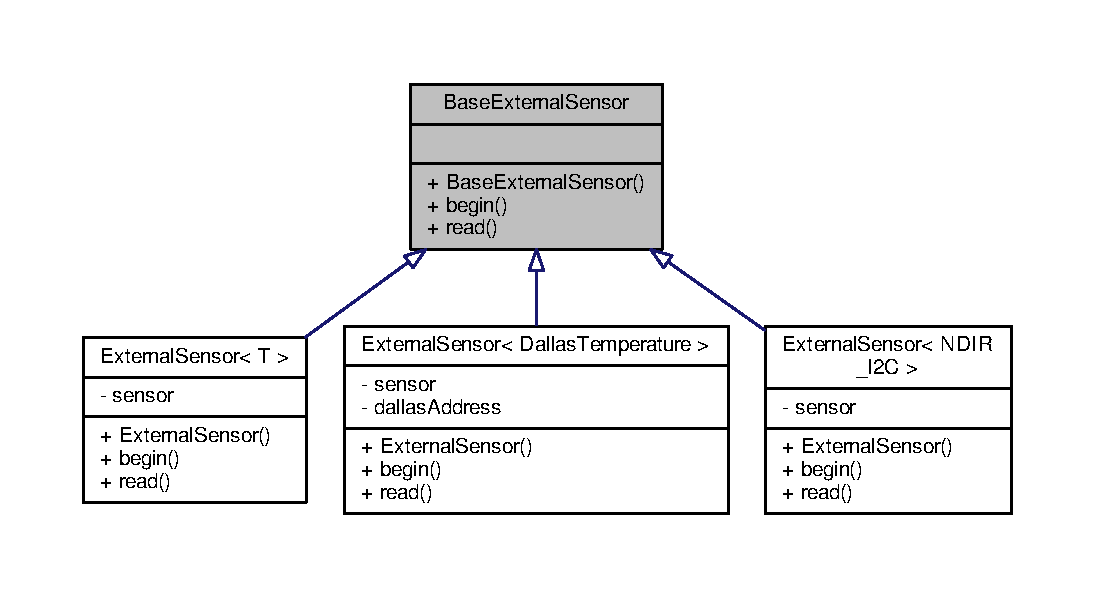
\includegraphics[width=350pt]{classBaseExternalSensor__inherit__graph}
\end{center}
\end{figure}


Collaboration diagram for Base\+External\+Sensor\+:
\nopagebreak
\begin{figure}[H]
\begin{center}
\leavevmode
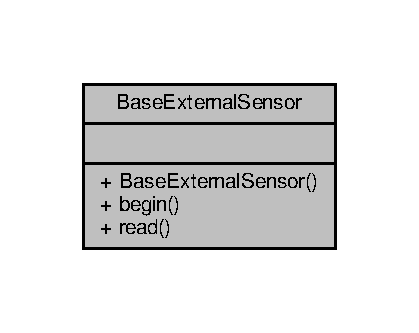
\includegraphics[width=201pt]{classBaseExternalSensor__coll__graph}
\end{center}
\end{figure}
\subsection*{Public Member Functions}
\begin{DoxyCompactItemize}
\item 
\hyperlink{classBaseExternalSensor_a978d96a6563b646efb358c2790a9fc6f}{Base\+External\+Sensor} ()
\item 
virtual uint8\+\_\+t \hyperlink{classBaseExternalSensor_a87d132803d4f4fdd4e66332809f0c9a0}{begin} ()
\item 
virtual int \hyperlink{classBaseExternalSensor_a7e0a98f350148d7645031315657aa5ec}{read} ()
\end{DoxyCompactItemize}


\subsection{Detailed Description}
This class is a generic external Sensor it is a way to access real external sensor methods through run Time polymorphism. 

Definition at line 22 of file External\+Sensor.\+h.



\subsection{Constructor \& Destructor Documentation}
\mbox{\Hypertarget{classBaseExternalSensor_a978d96a6563b646efb358c2790a9fc6f}\label{classBaseExternalSensor_a978d96a6563b646efb358c2790a9fc6f}} 
\index{Base\+External\+Sensor@{Base\+External\+Sensor}!Base\+External\+Sensor@{Base\+External\+Sensor}}
\index{Base\+External\+Sensor@{Base\+External\+Sensor}!Base\+External\+Sensor@{Base\+External\+Sensor}}
\subsubsection{\texorpdfstring{Base\+External\+Sensor()}{BaseExternalSensor()}}
{\footnotesize\ttfamily Base\+External\+Sensor\+::\+Base\+External\+Sensor (\begin{DoxyParamCaption}{ }\end{DoxyParamCaption})\hspace{0.3cm}{\ttfamily [inline]}}

\hyperlink{classBaseExternalSensor_a978d96a6563b646efb358c2790a9fc6f}{Base\+External\+Sensor()}\+: Base class generic Constructor 

Definition at line 30 of file External\+Sensor.\+h.


\begin{DoxyCode}
31     \{
32     
33     \}
\end{DoxyCode}


\subsection{Member Function Documentation}
\mbox{\Hypertarget{classBaseExternalSensor_a87d132803d4f4fdd4e66332809f0c9a0}\label{classBaseExternalSensor_a87d132803d4f4fdd4e66332809f0c9a0}} 
\index{Base\+External\+Sensor@{Base\+External\+Sensor}!begin@{begin}}
\index{begin@{begin}!Base\+External\+Sensor@{Base\+External\+Sensor}}
\subsubsection{\texorpdfstring{begin()}{begin()}}
{\footnotesize\ttfamily virtual uint8\+\_\+t Base\+External\+Sensor\+::begin (\begin{DoxyParamCaption}{ }\end{DoxyParamCaption})\hspace{0.3cm}{\ttfamily [inline]}, {\ttfamily [virtual]}}

\hyperlink{classBaseExternalSensor_a87d132803d4f4fdd4e66332809f0c9a0}{begin()}\+: Base class virtual generic begin method

\begin{DoxyReturn}{Returns}
generic value as it\textquotesingle{}s not supposed to be used 
\end{DoxyReturn}


Reimplemented in \hyperlink{classExternalSensor_3_01DallasTemperature_01_4_ac5275129b05e2ff8df45d5b222a661d9}{External\+Sensor$<$ Dallas\+Temperature $>$}, \hyperlink{classExternalSensor_3_01NDIR__I2C_01_4_ac6f3614d94968ef0cc11b2b4d69cef03}{External\+Sensor$<$ N\+D\+I\+R\+\_\+\+I2\+C $>$}, and \hyperlink{classExternalSensor_ab6fe1379d55b656a048e0fba1e0a32e6}{External\+Sensor$<$ T $>$}.



Definition at line 42 of file External\+Sensor.\+h.



Referenced by External\+Sensors\+::begin().


\begin{DoxyCode}
43     \{
44 
45         \textcolor{keywordflow}{return}(-2);
46     \}
\end{DoxyCode}
Here is the caller graph for this function\+:
\nopagebreak
\begin{figure}[H]
\begin{center}
\leavevmode
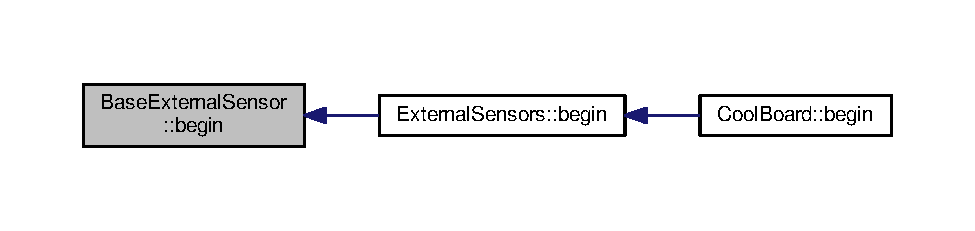
\includegraphics[width=350pt]{classBaseExternalSensor_a87d132803d4f4fdd4e66332809f0c9a0_icgraph}
\end{center}
\end{figure}
\mbox{\Hypertarget{classBaseExternalSensor_a7e0a98f350148d7645031315657aa5ec}\label{classBaseExternalSensor_a7e0a98f350148d7645031315657aa5ec}} 
\index{Base\+External\+Sensor@{Base\+External\+Sensor}!read@{read}}
\index{read@{read}!Base\+External\+Sensor@{Base\+External\+Sensor}}
\subsubsection{\texorpdfstring{read()}{read()}}
{\footnotesize\ttfamily virtual int Base\+External\+Sensor\+::read (\begin{DoxyParamCaption}{ }\end{DoxyParamCaption})\hspace{0.3cm}{\ttfamily [inline]}, {\ttfamily [virtual]}}

\hyperlink{classBaseExternalSensor_a7e0a98f350148d7645031315657aa5ec}{read()}\+: Base class virtual generic read method

\begin{DoxyReturn}{Returns}
generic value as it is not supposed to be used 
\end{DoxyReturn}


Reimplemented in \hyperlink{classExternalSensor_3_01DallasTemperature_01_4_a127ead06440ec972c22db2abeb8e2b51}{External\+Sensor$<$ Dallas\+Temperature $>$}, \hyperlink{classExternalSensor_3_01NDIR__I2C_01_4_add67f5ecaf47d2ee675e8299aee7322d}{External\+Sensor$<$ N\+D\+I\+R\+\_\+\+I2\+C $>$}, and \hyperlink{classExternalSensor_a6dbf2d6b1c183740ce0f153d6e43ccb2}{External\+Sensor$<$ T $>$}.



Definition at line 57 of file External\+Sensor.\+h.


\begin{DoxyCode}
58     \{
59 
60         \textcolor{keywordflow}{return}(-1);
61     \}
\end{DoxyCode}


The documentation for this class was generated from the following file\+:\begin{DoxyCompactItemize}
\item 
\hyperlink{ExternalSensor_8h}{External\+Sensor.\+h}\end{DoxyCompactItemize}

\hypertarget{classCoolBoard}{}\section{Cool\+Board Class Reference}
\label{classCoolBoard}\index{Cool\+Board@{Cool\+Board}}


This class manages the \hyperlink{classCoolBoard}{Cool\+Board} and all of Its functions.  




{\ttfamily \#include $<$Cool\+Board.\+h$>$}



Collaboration diagram for Cool\+Board\+:
\nopagebreak
\begin{figure}[H]
\begin{center}
\leavevmode
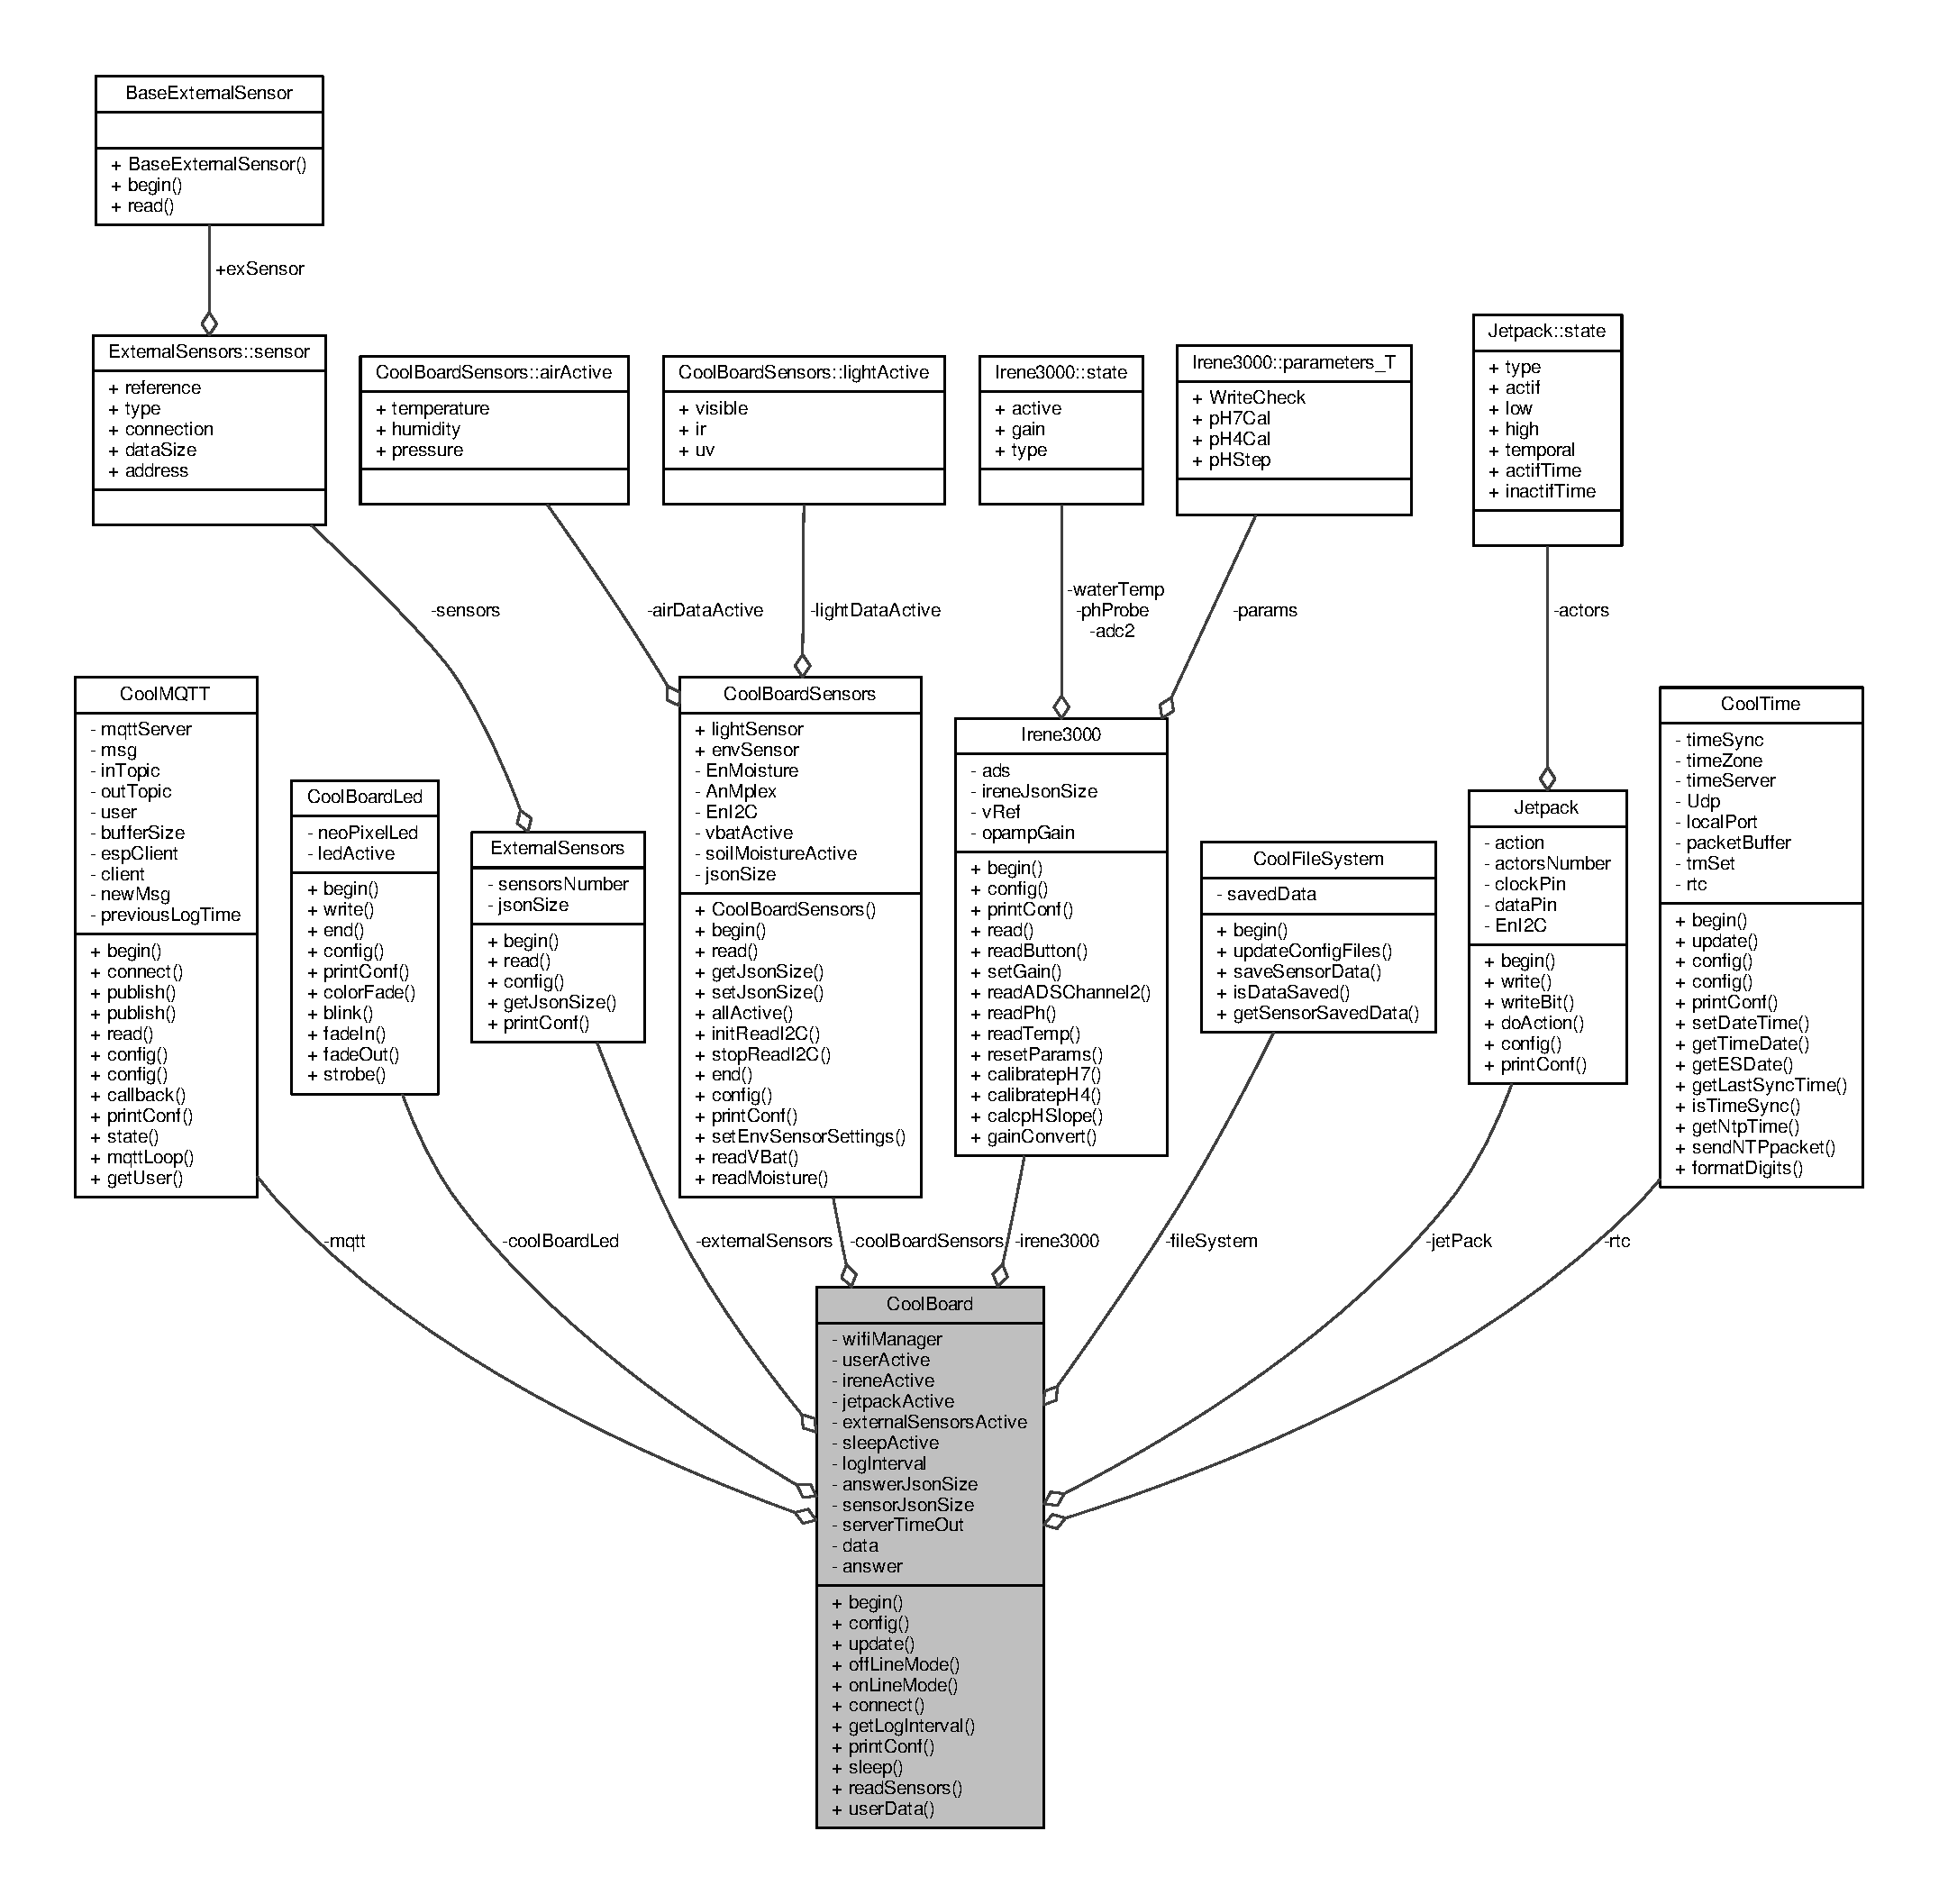
\includegraphics[width=350pt]{classCoolBoard__coll__graph}
\end{center}
\end{figure}
\subsection*{Public Member Functions}
\begin{DoxyCompactItemize}
\item 
void \hyperlink{classCoolBoard_acba7c5aef7268b2c0044bdb54d3b9d76}{begin} ()
\item 
bool \hyperlink{classCoolBoard_a583a874c09c07e70a6eb9229fc4beddb}{config} ()
\item 
void \hyperlink{classCoolBoard_a8612756d3f73198cdde857a66f0fe690}{update} (const char $\ast$\hyperlink{classCoolBoard_a7b835fafd449e5282f7f91d787a2dc15}{answer})
\item 
void \hyperlink{classCoolBoard_ae6b5e1274d760462290192acea4adca8}{off\+Line\+Mode} ()
\item 
void \hyperlink{classCoolBoard_aa0bbc4bc605e35618d18e68795c61363}{on\+Line\+Mode} ()
\item 
int \hyperlink{classCoolBoard_a519de78b807f8ec6463ff484eb925918}{connect} ()
\item 
unsigned long \hyperlink{classCoolBoard_a7508e029f2ee17bb747ffab599285e0d}{get\+Log\+Interval} ()
\item 
void \hyperlink{classCoolBoard_a486507b8f0981d3cc671ed31c2145755}{print\+Conf} ()
\item 
void \hyperlink{classCoolBoard_a069952cdcb2e7f68518aa429eceadb6e}{sleep} (unsigned long interval)
\item 
String \hyperlink{classCoolBoard_ad03abdce2e65f520bbf2cff0f2d083cf}{read\+Sensors} ()
\item 
String \hyperlink{classCoolBoard_ae7358fb6e623cfc81b775f5f1734909b}{user\+Data} ()
\end{DoxyCompactItemize}
\subsection*{Private Attributes}
\begin{DoxyCompactItemize}
\item 
\hyperlink{classCoolFileSystem}{Cool\+File\+System} \hyperlink{classCoolBoard_a42c2586fbb13ff7f06538e9284e8538d}{file\+System}
\item 
\hyperlink{classCoolBoardSensors}{Cool\+Board\+Sensors} \hyperlink{classCoolBoard_af102be5288bd7f7a8e59b13f86e26a00}{cool\+Board\+Sensors}
\item 
\hyperlink{classCoolBoardLed}{Cool\+Board\+Led} \hyperlink{classCoolBoard_a1b1d3c684a5baa56b08486e192fd8e97}{cool\+Board\+Led}
\item 
\hyperlink{classCoolTime}{Cool\+Time} \hyperlink{classCoolBoard_a50d2a6716879d64a85f3c6b44ad63275}{rtc}
\item 
\hyperlink{classCoolWifi}{Cool\+Wifi} \hyperlink{classCoolBoard_acd88e6003606b47479ebba81e4aceeca}{wifi\+Manager}
\item 
\hyperlink{classCoolMQTT}{Cool\+M\+Q\+TT} \hyperlink{classCoolBoard_a2399f44d7c23c1149a335cb3b46d90f1}{mqtt}
\item 
\hyperlink{classJetpack}{Jetpack} \hyperlink{classCoolBoard_a30b1357881b01ccbec676856a91e48e9}{jet\+Pack}
\item 
\hyperlink{classIrene3000}{Irene3000} \hyperlink{classCoolBoard_ad103718ce316006c4695b8eb312eaf11}{irene3000}
\item 
\hyperlink{classExternalSensors}{External\+Sensors} \hyperlink{classCoolBoard_a09e26264839c65873eb56af476eff6b2}{external\+Sensors}
\item 
bool \hyperlink{classCoolBoard_a6395459131d6889a3005f79c7a35e964}{user\+Active} =0
\item 
bool \hyperlink{classCoolBoard_a9c3f7ac625481ee2ae802a25d97a4ae0}{irene\+Active} =0
\item 
bool \hyperlink{classCoolBoard_a9be03a913d26e558328935ca3b59a75e}{jetpack\+Active} =0
\item 
bool \hyperlink{classCoolBoard_a638b00b76aeb819ecfd4c10b8cdd7bb7}{external\+Sensors\+Active} =0
\item 
bool \hyperlink{classCoolBoard_a0a51b2287139f66c738101fb53139230}{sleep\+Active} =0
\item 
unsigned long \hyperlink{classCoolBoard_a84bc94413b64973e4aba8c467c97006c}{log\+Interval} =1
\item 
int \hyperlink{classCoolBoard_a7a8d8d3d316220cdd049cd63c1aa8fe6}{server\+Time\+Out} =180
\item 
String \hyperlink{classCoolBoard_a427fb753dd8575bdf821c70a5c63d695}{data} =\char`\"{}\char`\"{}
\item 
String \hyperlink{classCoolBoard_a7b835fafd449e5282f7f91d787a2dc15}{answer} =\char`\"{}\char`\"{}
\end{DoxyCompactItemize}


\subsection{Detailed Description}
This class manages the \hyperlink{classCoolBoard}{Cool\+Board} and all of Its functions. 

Definition at line 33 of file Cool\+Board.\+h.



\subsection{Member Function Documentation}
\mbox{\Hypertarget{classCoolBoard_acba7c5aef7268b2c0044bdb54d3b9d76}\label{classCoolBoard_acba7c5aef7268b2c0044bdb54d3b9d76}} 
\index{Cool\+Board@{Cool\+Board}!begin@{begin}}
\index{begin@{begin}!Cool\+Board@{Cool\+Board}}
\subsubsection{\texorpdfstring{begin()}{begin()}}
{\footnotesize\ttfamily void Cool\+Board\+::begin (\begin{DoxyParamCaption}{ }\end{DoxyParamCaption})}

\hyperlink{classCoolBoard_acba7c5aef7268b2c0044bdb54d3b9d76}{Cool\+Board\+::begin()}\+: This method is provided to configure and start the used Cool\+Kit Parts. It also starts the first connection try If Serial is enabled,it prints the configuration of the used parts. 

Definition at line 37 of file Cool\+Board.\+cpp.



References Jetpack\+::begin(), Cool\+M\+Q\+T\+T\+::begin(), External\+Sensors\+::begin(), Cool\+Wifi\+::begin(), Cool\+Board\+Sensors\+::begin(), Cool\+Time\+::begin(), Irene3000\+::begin(), Cool\+Board\+Led\+::blink(), Jetpack\+::config(), External\+Sensors\+::config(), Cool\+Wifi\+::config(), Cool\+M\+Q\+T\+T\+::config(), Cool\+Time\+::config(), Irene3000\+::config(), Cool\+Board\+Sensors\+::config(), connect(), cool\+Board\+Led, cool\+Board\+Sensors, external\+Sensors, external\+Sensors\+Active, Cool\+Board\+Led\+::fade\+Out(), irene3000, irene\+Active, jet\+Pack, jetpack\+Active, mqtt, Cool\+Board\+Led\+::print\+Conf(), Jetpack\+::print\+Conf(), External\+Sensors\+::print\+Conf(), Cool\+M\+Q\+T\+T\+::print\+Conf(), Cool\+Wifi\+::print\+Conf(), Cool\+Time\+::print\+Conf(), Irene3000\+::print\+Conf(), Cool\+Board\+Sensors\+::print\+Conf(), rtc, wifi\+Manager, and Cool\+Board\+Led\+::write().


\begin{DoxyCode}
38 \{
39 
40 \textcolor{preprocessor}{#if DEBUG == 1}
41 
42     Serial.println( F(\textcolor{stringliteral}{"Starting the CoolBoard  "})  );
43     Serial.println( F(\textcolor{stringliteral}{"Entering CoolBoard.begin() "})  );
44     Serial.println();
45 \textcolor{preprocessor}{#endif  }
46     \hyperlink{classCoolBoard_a1b1d3c684a5baa56b08486e192fd8e97}{coolBoardLed}.\hyperlink{classCoolBoardLed_a8ed3053a36f0ed4a131f43b5b17efb61}{printConf}();
47     delay(100);
48     
49     \hyperlink{classCoolBoard_a1b1d3c684a5baa56b08486e192fd8e97}{coolBoardLed}.\hyperlink{classCoolBoardLed_a30fadd4cbec17ceea428bf7a32207e87}{write}(255,128,0);\textcolor{comment}{//orange}
50     
51     \hyperlink{classCoolBoard_af102be5288bd7f7a8e59b13f86e26a00}{coolBoardSensors}.\hyperlink{classCoolBoardSensors_a9a218895c5423375c33c08f2c56fb23a}{config}();
52     \hyperlink{classCoolBoard_af102be5288bd7f7a8e59b13f86e26a00}{coolBoardSensors}.\hyperlink{classCoolBoardSensors_a97095823ef7c8f5290812f1405b966b3}{begin}();
53     \hyperlink{classCoolBoard_af102be5288bd7f7a8e59b13f86e26a00}{coolBoardSensors}.\hyperlink{classCoolBoardSensors_af6fd79505815b204c178617ecf54c873}{printConf}();
54     delay(100);
55     
56     \hyperlink{classCoolBoard_acd88e6003606b47479ebba81e4aceeca}{wifiManager}.\hyperlink{classCoolWifi_a4eb2f6b9b09dd588964b88b6c70122c0}{config}();
57     \hyperlink{classCoolBoard_acd88e6003606b47479ebba81e4aceeca}{wifiManager}.\hyperlink{classCoolWifi_a46942fed90e475112cc10b78a32e7aaa}{begin}();
58     \hyperlink{classCoolBoard_acd88e6003606b47479ebba81e4aceeca}{wifiManager}.\hyperlink{classCoolWifi_a9e6105c6d13d35ec510f6633da9e0223}{printConf}();
59     delay(100);
60 
61     \hyperlink{classCoolBoard_a2399f44d7c23c1149a335cb3b46d90f1}{mqtt}.\hyperlink{classCoolMQTT_a9b703de4f1358f0ee7a5e8c44979c648}{config}();
62     \hyperlink{classCoolBoard_a2399f44d7c23c1149a335cb3b46d90f1}{mqtt}.\hyperlink{classCoolMQTT_ac9248808641ebf3054ed0620ea9d0100}{begin}();
63     \hyperlink{classCoolBoard_a2399f44d7c23c1149a335cb3b46d90f1}{mqtt}.\hyperlink{classCoolMQTT_a40553a0ad4b5ecf1cb4411ab54ca85fb}{printConf}();
64     delay(100);
65 
66     \textcolor{keywordflow}{if} (\hyperlink{classCoolBoard_a9be03a913d26e558328935ca3b59a75e}{jetpackActive})
67     \{
68         \hyperlink{classCoolBoard_a30b1357881b01ccbec676856a91e48e9}{jetPack}.\hyperlink{classJetpack_ab065ee83e244265a2223a22f3ee4a719}{config}();
69         \hyperlink{classCoolBoard_a30b1357881b01ccbec676856a91e48e9}{jetPack}.\hyperlink{classJetpack_a5a53e1ebf7aaf3bf3e0d37ea64ca09a7}{begin}();
70         \hyperlink{classCoolBoard_a30b1357881b01ccbec676856a91e48e9}{jetPack}.\hyperlink{classJetpack_ac54a7bb4f9166bee32052253d9b1d306}{printConf}();
71         delay(100);
72     \}
73 
74     \textcolor{keywordflow}{if} (\hyperlink{classCoolBoard_a9c3f7ac625481ee2ae802a25d97a4ae0}{ireneActive})
75     \{
76         \hyperlink{classCoolBoard_ad103718ce316006c4695b8eb312eaf11}{irene3000}.\hyperlink{classIrene3000_afed5c35e4b23963c157847ef27c11e9c}{config}();
77         \hyperlink{classCoolBoard_ad103718ce316006c4695b8eb312eaf11}{irene3000}.\hyperlink{classIrene3000_ad5891806c500ae1007afe52b9e304c2b}{begin}();
78         \hyperlink{classCoolBoard_ad103718ce316006c4695b8eb312eaf11}{irene3000}.\hyperlink{classIrene3000_a7bc2414100b5e19eacc6630fa34b2654}{printConf}();
79         delay(100);
80     \}
81 
82     \textcolor{keywordflow}{if} (\hyperlink{classCoolBoard_a638b00b76aeb819ecfd4c10b8cdd7bb7}{externalSensorsActive})
83     \{
84         \hyperlink{classCoolBoard_a09e26264839c65873eb56af476eff6b2}{externalSensors}.\hyperlink{classExternalSensors_a862a4bd11346b37270d0244c2adabe5a}{config}();
85         \hyperlink{classCoolBoard_a09e26264839c65873eb56af476eff6b2}{externalSensors}.\hyperlink{classExternalSensors_a58ede0d786a86417254708870f04a21e}{begin}();
86         \hyperlink{classCoolBoard_a09e26264839c65873eb56af476eff6b2}{externalSensors}.\hyperlink{classExternalSensors_a78c2bf55084435dd51d3c559b2d3c6f3}{printConf}();
87         delay(100);
88     \}
89     
90     \hyperlink{classCoolBoard_a1b1d3c684a5baa56b08486e192fd8e97}{coolBoardLed}.\hyperlink{classCoolBoardLed_a93d545679237e8cc858324367149775c}{fadeOut}(255,128,0,0.5);\textcolor{comment}{//orange}
91 
92     this->\hyperlink{classCoolBoard_a519de78b807f8ec6463ff484eb925918}{connect}();
93     delay(100);
94 
95     \hyperlink{classCoolBoard_a50d2a6716879d64a85f3c6b44ad63275}{rtc}.\hyperlink{classCoolTime_a87c28260c1bc77091162cbcf1ee2e129}{config}();
96     \hyperlink{classCoolBoard_a50d2a6716879d64a85f3c6b44ad63275}{rtc}.\hyperlink{classCoolTime_ab1976cf718b950bc31e003c3323b8adb}{begin}();
97     \hyperlink{classCoolBoard_a50d2a6716879d64a85f3c6b44ad63275}{rtc}.\hyperlink{classCoolTime_af355e7f9b3898211cd2ff25eab5933b1}{printConf}();
98     delay(100);
99     
100     \hyperlink{classCoolBoard_a1b1d3c684a5baa56b08486e192fd8e97}{coolBoardLed}.\hyperlink{classCoolBoardLed_a96e1ea13003eee34c9dbcef340404426}{blink}(0,255,0,0.5);\textcolor{comment}{//green}
101 
102 \}
\end{DoxyCode}
Here is the call graph for this function\+:\nopagebreak
\begin{figure}[H]
\begin{center}
\leavevmode
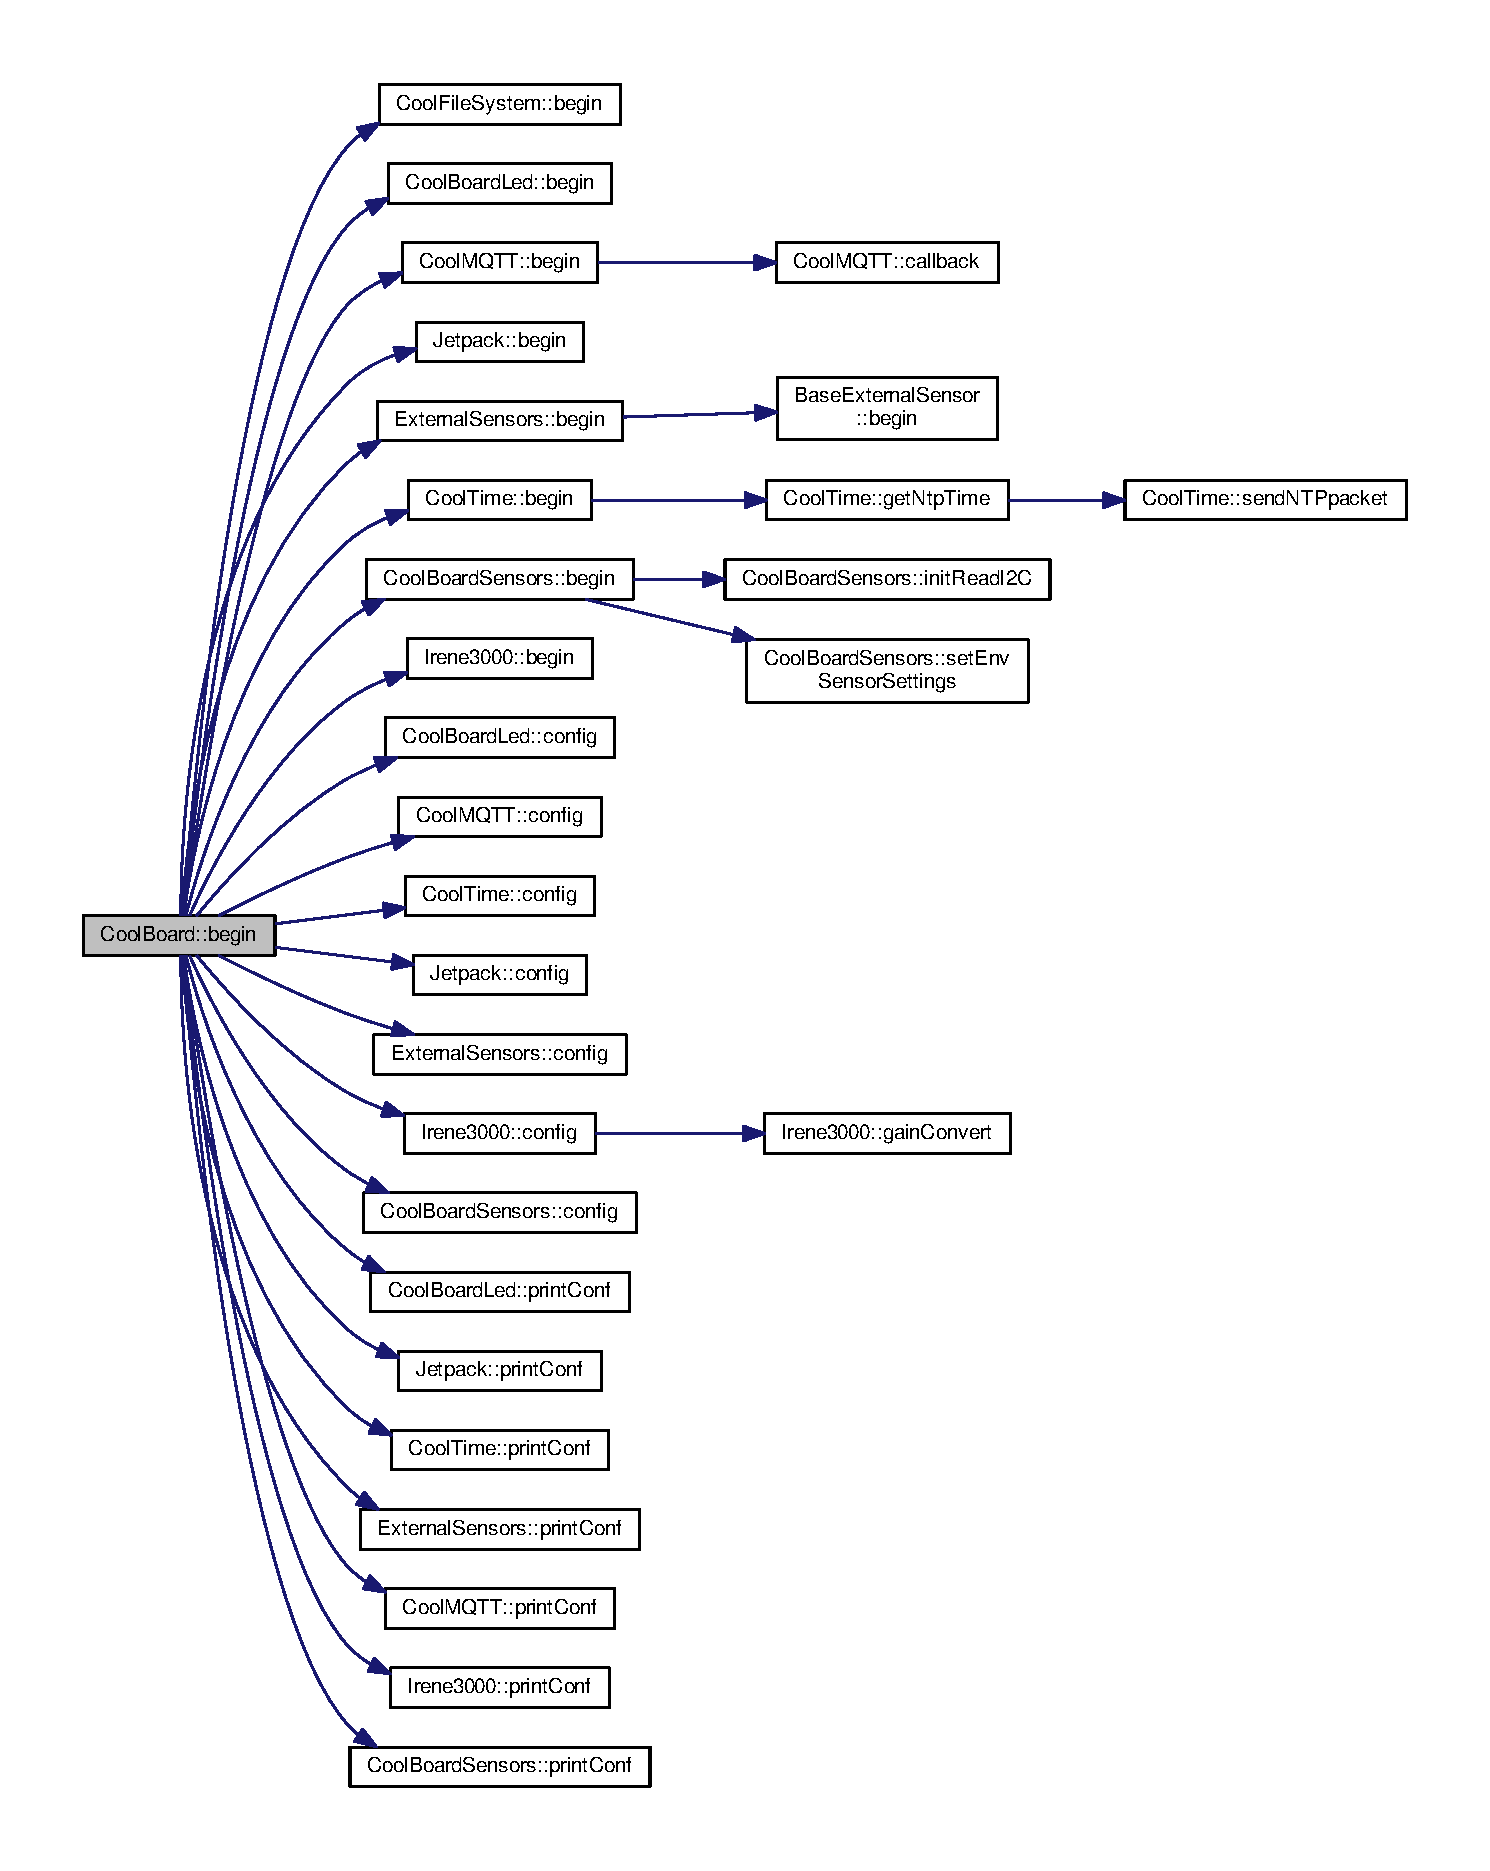
\includegraphics[width=350pt]{classCoolBoard_acba7c5aef7268b2c0044bdb54d3b9d76_cgraph}
\end{center}
\end{figure}
\mbox{\Hypertarget{classCoolBoard_a583a874c09c07e70a6eb9229fc4beddb}\label{classCoolBoard_a583a874c09c07e70a6eb9229fc4beddb}} 
\index{Cool\+Board@{Cool\+Board}!config@{config}}
\index{config@{config}!Cool\+Board@{Cool\+Board}}
\subsubsection{\texorpdfstring{config()}{config()}}
{\footnotesize\ttfamily bool Cool\+Board\+::config (\begin{DoxyParamCaption}{ }\end{DoxyParamCaption})}

\hyperlink{classCoolBoard_a583a874c09c07e70a6eb9229fc4beddb}{Cool\+Board\+::config()}\+: This method is provided to configure the \hyperlink{classCoolBoard}{Cool\+Board} \+: -\/log interval -\/irene3000 activated/deactivated -\/jetpack activated/deactivated -\/external Sensors activated/deactivated -\/mqtt server timeout

\begin{DoxyReturn}{Returns}
true if configuration is done, false otherwise 
\end{DoxyReturn}


Definition at line 486 of file Cool\+Board.\+cpp.



References Cool\+File\+System\+::begin(), Cool\+Board\+Led\+::begin(), Cool\+Board\+Led\+::blink(), Cool\+Board\+Led\+::config(), cool\+Board\+Led, external\+Sensors\+Active, Cool\+Board\+Led\+::fade\+In(), Cool\+Board\+Led\+::fade\+Out(), file\+System, irene\+Active, jetpack\+Active, log\+Interval, server\+Time\+Out, sleep\+Active, Cool\+Board\+Led\+::strobe(), and user\+Active.


\begin{DoxyCode}
487 \{
488 
489 \textcolor{preprocessor}{#if DEBUG == 1}
490 
491     Serial.println( F(\textcolor{stringliteral}{"Entering CoolBoard.config() "}) );
492     Serial.println();
493 
494 \textcolor{preprocessor}{#endif}
495 
496     \textcolor{comment}{//open file system}
497     \hyperlink{classCoolBoard_a42c2586fbb13ff7f06538e9284e8538d}{fileSystem}.\hyperlink{classCoolFileSystem_a6ba6f666ed4c530174f8569d2c636748}{begin}();
498     
499     \textcolor{comment}{//start the led}
500     \hyperlink{classCoolBoard_a1b1d3c684a5baa56b08486e192fd8e97}{coolBoardLed}.\hyperlink{classCoolBoardLed_a1b60e5e30bea96c49ed62ed1bf1ffc8b}{config}();
501     \hyperlink{classCoolBoard_a1b1d3c684a5baa56b08486e192fd8e97}{coolBoardLed}.\hyperlink{classCoolBoardLed_ae3cbde8affcc6f011cbd698c8ef911f6}{begin}();
502     \hyperlink{classCoolBoard_a1b1d3c684a5baa56b08486e192fd8e97}{coolBoardLed}.\hyperlink{classCoolBoardLed_ab778f5e7bed0ab74e3906d82110493c3}{fadeIn}(243,171,46,0.5);\textcolor{comment}{//shade of orange     }
503 
504     
505     \textcolor{comment}{//open configuration file}
506     File configFile = SPIFFS.open(\textcolor{stringliteral}{"/coolBoardConfig.json"}, \textcolor{stringliteral}{"r"});
507     
508     \textcolor{keywordflow}{if} (!configFile)
509 
510     \{
511     
512 \textcolor{preprocessor}{    #if DEBUG == 1}
513 
514         Serial.println( F(\textcolor{stringliteral}{"failed to read /coolBoardConfig.json  "}) );
515 
516 \textcolor{preprocessor}{    #endif}
517         \hyperlink{classCoolBoard_a1b1d3c684a5baa56b08486e192fd8e97}{coolBoardLed}.\hyperlink{classCoolBoardLed_a96e1ea13003eee34c9dbcef340404426}{blink}(255,0,0,0.5);\textcolor{comment}{//shade of red     }
518         \textcolor{keywordflow}{return}(\textcolor{keyword}{false});
519     \}
520 
521     \textcolor{keywordflow}{else}
522     \{
523         \textcolor{keywordtype}{size\_t} size = configFile.size();
524 
525         \textcolor{comment}{// Allocate a buffer to store contents of the file.}
526         std::unique\_ptr < char[] > buf(\textcolor{keyword}{new} \textcolor{keywordtype}{char}[size]);
527 
528         configFile.readBytes(buf.get(), size);
529 
530         DynamicJsonBuffer jsonBuffer;
531 
532         JsonObject & json = jsonBuffer.parseObject(buf.get());
533 
534         \textcolor{keywordflow}{if} (!json.success())
535         \{
536         
537 \textcolor{preprocessor}{        #if DEBUG == 1}
538 
539             Serial.println( F(\textcolor{stringliteral}{"failed to parse CoolBoard Config json object "}) );
540     
541 \textcolor{preprocessor}{        #endif}
542             \hyperlink{classCoolBoard_a1b1d3c684a5baa56b08486e192fd8e97}{coolBoardLed}.\hyperlink{classCoolBoardLed_a96e1ea13003eee34c9dbcef340404426}{blink}(255,0,0,0.5);\textcolor{comment}{//shade of red     }
543             \textcolor{keywordflow}{return}(\textcolor{keyword}{false});
544         \}
545 
546         \textcolor{keywordflow}{else}
547         \{   
548         
549 \textcolor{preprocessor}{        #if DEBUG == 1}
550             
551             Serial.println( F(\textcolor{stringliteral}{"configuration json : "}) );
552             json.printTo(Serial);
553             Serial.println();
554             
555             Serial.print(F(\textcolor{stringliteral}{"jsonBuffer size : "}));
556             Serial.print(jsonBuffer.size());
557             Serial.println();
558 
559 \textcolor{preprocessor}{        #endif}
560             
561             \textcolor{comment}{//parsing userActive Key}
562             \textcolor{keywordflow}{if} (json[\textcolor{stringliteral}{"userActive"}].success())
563             \{
564                 \textcolor{keyword}{this} -> \hyperlink{classCoolBoard_a6395459131d6889a3005f79c7a35e964}{userActive} = json[\textcolor{stringliteral}{"userActive"}];
565             \}
566 
567             \textcolor{keywordflow}{else}
568             \{
569                 \textcolor{keyword}{this} -> \hyperlink{classCoolBoard_a6395459131d6889a3005f79c7a35e964}{userActive} = \textcolor{keyword}{this} -> \hyperlink{classCoolBoard_a6395459131d6889a3005f79c7a35e964}{userActive};
570             \}
571             json[\textcolor{stringliteral}{"userActive"}] = \textcolor{keyword}{this} -> \hyperlink{classCoolBoard_a6395459131d6889a3005f79c7a35e964}{userActive};
572 
573             \textcolor{comment}{//parsing logInterval key}
574             \textcolor{keywordflow}{if} (json[\textcolor{stringliteral}{"logInterval"}].success())
575             \{
576                 \textcolor{keyword}{this} -> \hyperlink{classCoolBoard_a84bc94413b64973e4aba8c467c97006c}{logInterval} = json[\textcolor{stringliteral}{"logInterval"}];
577             \}
578             \textcolor{keywordflow}{else}
579             \{
580                 \textcolor{keyword}{this} -> \hyperlink{classCoolBoard_a84bc94413b64973e4aba8c467c97006c}{logInterval} = \textcolor{keyword}{this} -> \hyperlink{classCoolBoard_a84bc94413b64973e4aba8c467c97006c}{logInterval};
581             \}
582             json[\textcolor{stringliteral}{"logInterval"}] = \textcolor{keyword}{this} -> \hyperlink{classCoolBoard_a84bc94413b64973e4aba8c467c97006c}{logInterval};
583             
584             \textcolor{comment}{//parsing ireneActive key           }
585             \textcolor{keywordflow}{if} (json[\textcolor{stringliteral}{"ireneActive"}].success())
586             \{
587                 \textcolor{keyword}{this} -> \hyperlink{classCoolBoard_a9c3f7ac625481ee2ae802a25d97a4ae0}{ireneActive} = json[\textcolor{stringliteral}{"ireneActive"}];
588             \}
589             \textcolor{keywordflow}{else}
590             \{
591                 \textcolor{keyword}{this} -> \hyperlink{classCoolBoard_a9c3f7ac625481ee2ae802a25d97a4ae0}{ireneActive} = \textcolor{keyword}{this} -> \hyperlink{classCoolBoard_a9c3f7ac625481ee2ae802a25d97a4ae0}{ireneActive};
592             \}
593             json[\textcolor{stringliteral}{"ireneActive"}] = \textcolor{keyword}{this} -> \hyperlink{classCoolBoard_a9c3f7ac625481ee2ae802a25d97a4ae0}{ireneActive};
594             
595             \textcolor{comment}{//parsing jetpackActive key}
596             \textcolor{keywordflow}{if} (json[\textcolor{stringliteral}{"jetpackActive"}].success())
597             \{
598                 \textcolor{keyword}{this} -> \hyperlink{classCoolBoard_a9be03a913d26e558328935ca3b59a75e}{jetpackActive} = json[\textcolor{stringliteral}{"jetpackActive"}];
599             \}
600             \textcolor{keywordflow}{else}
601             \{
602                 \textcolor{keyword}{this} -> \hyperlink{classCoolBoard_a9be03a913d26e558328935ca3b59a75e}{jetpackActive} = \textcolor{keyword}{this} -> \hyperlink{classCoolBoard_a9be03a913d26e558328935ca3b59a75e}{jetpackActive};
603             \}
604             json[\textcolor{stringliteral}{"jetpackActive"}] = \textcolor{keyword}{this} -> \hyperlink{classCoolBoard_a9be03a913d26e558328935ca3b59a75e}{jetpackActive};
605 
606             \textcolor{comment}{//parsing externalSensorsActive key}
607             \textcolor{keywordflow}{if} (json[\textcolor{stringliteral}{"externalSensorsActive"}].success())
608             \{
609                 \textcolor{keyword}{this} -> \hyperlink{classCoolBoard_a638b00b76aeb819ecfd4c10b8cdd7bb7}{externalSensorsActive} = json[\textcolor{stringliteral}{"externalSensorsActive"}];
610             \}
611             \textcolor{keywordflow}{else}
612             \{
613                 \textcolor{keyword}{this} -> \hyperlink{classCoolBoard_a638b00b76aeb819ecfd4c10b8cdd7bb7}{externalSensorsActive} = \textcolor{keyword}{this} -> 
      \hyperlink{classCoolBoard_a638b00b76aeb819ecfd4c10b8cdd7bb7}{externalSensorsActive};
614             \}
615             json[\textcolor{stringliteral}{"externalSensorsActive"}] = \textcolor{keyword}{this} -> \hyperlink{classCoolBoard_a638b00b76aeb819ecfd4c10b8cdd7bb7}{externalSensorsActive};
616 
617             \textcolor{comment}{//parsing serverTimeOut key}
618             \textcolor{keywordflow}{if} (json[\textcolor{stringliteral}{"serverTimeOut"}].success())
619             \{
620                 \textcolor{keyword}{this} -> \hyperlink{classCoolBoard_a7a8d8d3d316220cdd049cd63c1aa8fe6}{serverTimeOut} = json[\textcolor{stringliteral}{"serverTimeOut"}];
621             \}
622             \textcolor{keywordflow}{else}
623             \{
624                 \textcolor{keyword}{this} -> \hyperlink{classCoolBoard_a7a8d8d3d316220cdd049cd63c1aa8fe6}{serverTimeOut} = \textcolor{keyword}{this} -> \hyperlink{classCoolBoard_a7a8d8d3d316220cdd049cd63c1aa8fe6}{serverTimeOut};
625             \}
626             json[\textcolor{stringliteral}{"serverTimeOut"}] = \textcolor{keyword}{this} -> \hyperlink{classCoolBoard_a7a8d8d3d316220cdd049cd63c1aa8fe6}{serverTimeOut};
627             
628             \textcolor{comment}{//parsing sleepActive key}
629             \textcolor{keywordflow}{if} (json[\textcolor{stringliteral}{"sleepActive"}].success())
630             \{
631                 \textcolor{keyword}{this} -> \hyperlink{classCoolBoard_a0a51b2287139f66c738101fb53139230}{sleepActive} = json[\textcolor{stringliteral}{"sleepActive"}];
632             \}
633             \textcolor{keywordflow}{else}
634             \{
635                 \textcolor{keyword}{this} -> \hyperlink{classCoolBoard_a0a51b2287139f66c738101fb53139230}{sleepActive} = \textcolor{keyword}{this} -> \hyperlink{classCoolBoard_a0a51b2287139f66c738101fb53139230}{sleepActive};
636             \}
637             json[\textcolor{stringliteral}{"sleepActive"}] = \textcolor{keyword}{this} -> \hyperlink{classCoolBoard_a0a51b2287139f66c738101fb53139230}{sleepActive};
638 
639             \textcolor{comment}{//saving the current/correct configuration}
640             configFile.close();
641             configFile = SPIFFS.open(\textcolor{stringliteral}{"/coolBoardConfig.json"}, \textcolor{stringliteral}{"w"});
642             \textcolor{keywordflow}{if} (!configFile)
643             \{
644             
645 \textcolor{preprocessor}{            #if DEBUG == 1}
646 
647                 Serial.println( F(\textcolor{stringliteral}{"failed to write to /coolBoardConfig.json"}) );
648                 Serial.println();
649             
650 \textcolor{preprocessor}{            #endif}
651                 \hyperlink{classCoolBoard_a1b1d3c684a5baa56b08486e192fd8e97}{coolBoardLed}.\hyperlink{classCoolBoardLed_a96e1ea13003eee34c9dbcef340404426}{blink}(255,0,0,0.5);\textcolor{comment}{//shade of red     }
652                 \textcolor{keywordflow}{return}(\textcolor{keyword}{false});
653             \}
654 
655             json.printTo(configFile);
656             configFile.close();
657             \textcolor{keywordflow}{return}(\textcolor{keyword}{true});
658         \}
659     \}
660 
661     \hyperlink{classCoolBoard_a1b1d3c684a5baa56b08486e192fd8e97}{coolBoardLed}.\hyperlink{classCoolBoardLed_ad5f0de4c628cbfbf49896042831c64ad}{strobe}(243,171,46,0.5);\textcolor{comment}{//shade of orange}
662     
663     \hyperlink{classCoolBoard_a1b1d3c684a5baa56b08486e192fd8e97}{coolBoardLed}.\hyperlink{classCoolBoardLed_a93d545679237e8cc858324367149775c}{fadeOut}(243,171,46,0.5);\textcolor{comment}{//shade of orange               }
664 \}
\end{DoxyCode}
Here is the call graph for this function\+:\nopagebreak
\begin{figure}[H]
\begin{center}
\leavevmode
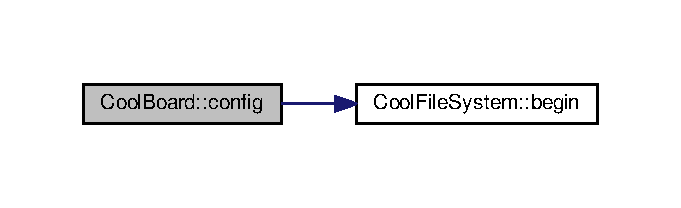
\includegraphics[width=330pt]{classCoolBoard_a583a874c09c07e70a6eb9229fc4beddb_cgraph}
\end{center}
\end{figure}
\mbox{\Hypertarget{classCoolBoard_a519de78b807f8ec6463ff484eb925918}\label{classCoolBoard_a519de78b807f8ec6463ff484eb925918}} 
\index{Cool\+Board@{Cool\+Board}!connect@{connect}}
\index{connect@{connect}!Cool\+Board@{Cool\+Board}}
\subsubsection{\texorpdfstring{connect()}{connect()}}
{\footnotesize\ttfamily int Cool\+Board\+::connect (\begin{DoxyParamCaption}{ }\end{DoxyParamCaption})}

\hyperlink{classCoolBoard_a519de78b807f8ec6463ff484eb925918}{Cool\+Board\+::connect()}\+: This method is provided to manage the network connection and the mqtt connection.

\begin{DoxyReturn}{Returns}
mqtt client state 
\end{DoxyReturn}


Definition at line 111 of file Cool\+Board.\+cpp.



References Cool\+Board\+Led\+::blink(), Cool\+M\+Q\+T\+T\+::connect(), Cool\+Wifi\+::connect(), cool\+Board\+Led, get\+Log\+Interval(), mqtt, Cool\+Wifi\+::state(), Cool\+M\+Q\+T\+T\+::state(), wifi\+Manager, and Cool\+Board\+Led\+::write().



Referenced by begin().


\begin{DoxyCode}
112 \{
113 
114 \textcolor{preprocessor}{#if DEBUG == 1  }
115 
116     Serial.println( F(\textcolor{stringliteral}{"Entering CoolBoard.connect "}) );
117     Serial.println();
118     Serial.println( F(\textcolor{stringliteral}{"Connecting the CoolBoard  "}) );
119     delay(100);
120 
121 \textcolor{preprocessor}{#endif}
122     \hyperlink{classCoolBoard_a1b1d3c684a5baa56b08486e192fd8e97}{coolBoardLed}.\hyperlink{classCoolBoardLed_a30fadd4cbec17ceea428bf7a32207e87}{write}(0,0,255);\textcolor{comment}{//blue}
123 
124     \textcolor{keywordflow}{if} (\hyperlink{classCoolBoard_acd88e6003606b47479ebba81e4aceeca}{wifiManager}.\hyperlink{classCoolWifi_a1c7b4d82a4098d346e7593dce92039fa}{state}() != WL\_CONNECTED)
125     \{       
126     
127 \textcolor{preprocessor}{    #if DEBUG == 1      }
128 
129         Serial.println( F(\textcolor{stringliteral}{"CoolBoard not connected to WiFi "}) );
130         Serial.println( F(\textcolor{stringliteral}{"Launching CoolWifi"}) );
131         Serial.println();
132 
133 \textcolor{preprocessor}{    #endif}
134         \hyperlink{classCoolBoard_acd88e6003606b47479ebba81e4aceeca}{wifiManager}.\hyperlink{classCoolWifi_ad060353050f40d032a2dbf9e54a768bf}{connect}();
135         delay(100);
136     \}
137 
138 
139     
140     \textcolor{keywordflow}{if} (\hyperlink{classCoolBoard_a2399f44d7c23c1149a335cb3b46d90f1}{mqtt}.\hyperlink{classCoolMQTT_a5d003307eff78efbd585e42b43b72b6d}{state}() != 0)
141     \{   
142     
143 \textcolor{preprocessor}{    #if DEBUG == 1  }
144     
145         Serial.println( F(\textcolor{stringliteral}{"CoolBoard not connected to MQTT "}) );
146         Serial.println( F(\textcolor{stringliteral}{"Launching mqtt.connect()"}) );
147         Serial.println();
148 
149 \textcolor{preprocessor}{    #endif  }
150         \textcolor{comment}{//logInterval in seconds}
151         \hyperlink{classCoolBoard_a2399f44d7c23c1149a335cb3b46d90f1}{mqtt}.\hyperlink{classCoolMQTT_a50075d0ab23a327ab897fd6adad20eda}{connect}(\textcolor{keyword}{this} -> \hyperlink{classCoolBoard_a7508e029f2ee17bb747ffab599285e0d}{getLogInterval}());
152         delay(100);
153         
154     \}
155     
156 \textcolor{preprocessor}{#if DEBUG == 1}
157 
158     Serial.println( F(\textcolor{stringliteral}{"mqtt state is :"}) );
159     Serial.println(\hyperlink{classCoolBoard_a2399f44d7c23c1149a335cb3b46d90f1}{mqtt}.\hyperlink{classCoolMQTT_a5d003307eff78efbd585e42b43b72b6d}{state}());
160     Serial.println();
161     delay(100);
162 
163 \textcolor{preprocessor}{#endif}
164 
165     \hyperlink{classCoolBoard_a1b1d3c684a5baa56b08486e192fd8e97}{coolBoardLed}.\hyperlink{classCoolBoardLed_a96e1ea13003eee34c9dbcef340404426}{blink}(0,0,255,0.5);\textcolor{comment}{//blue}
166 
167     \textcolor{keywordflow}{return}(\hyperlink{classCoolBoard_a2399f44d7c23c1149a335cb3b46d90f1}{mqtt}.\hyperlink{classCoolMQTT_a5d003307eff78efbd585e42b43b72b6d}{state}());
168 \}
\end{DoxyCode}
Here is the call graph for this function\+:\nopagebreak
\begin{figure}[H]
\begin{center}
\leavevmode
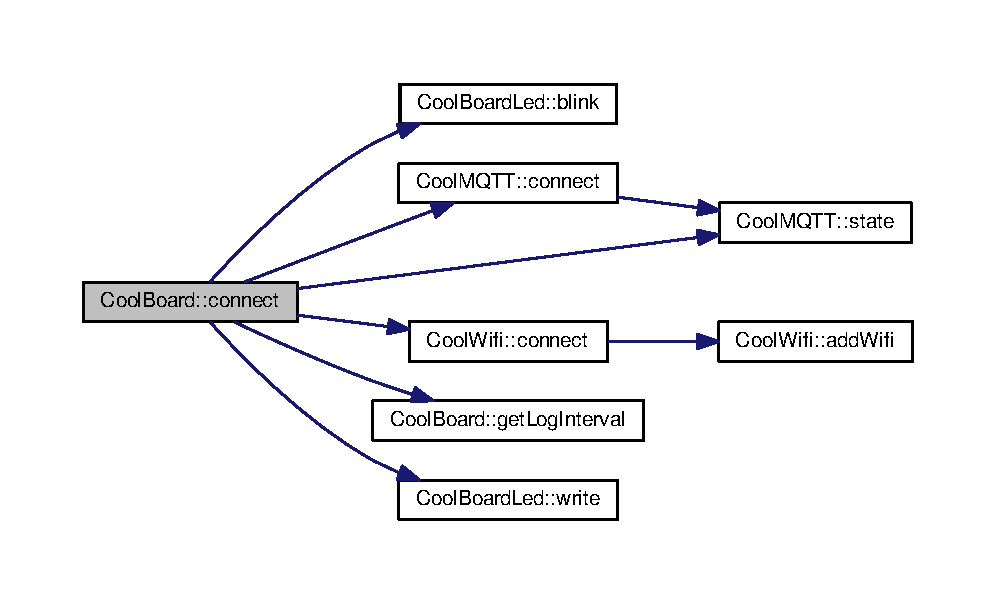
\includegraphics[width=350pt]{classCoolBoard_a519de78b807f8ec6463ff484eb925918_cgraph}
\end{center}
\end{figure}
Here is the caller graph for this function\+:\nopagebreak
\begin{figure}[H]
\begin{center}
\leavevmode
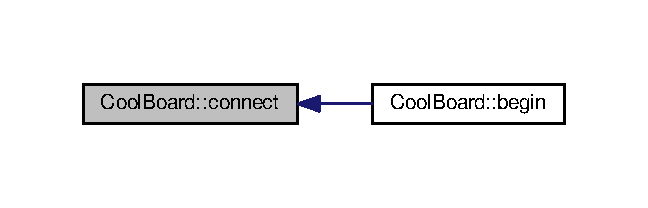
\includegraphics[width=311pt]{classCoolBoard_a519de78b807f8ec6463ff484eb925918_icgraph}
\end{center}
\end{figure}
\mbox{\Hypertarget{classCoolBoard_a7508e029f2ee17bb747ffab599285e0d}\label{classCoolBoard_a7508e029f2ee17bb747ffab599285e0d}} 
\index{Cool\+Board@{Cool\+Board}!get\+Log\+Interval@{get\+Log\+Interval}}
\index{get\+Log\+Interval@{get\+Log\+Interval}!Cool\+Board@{Cool\+Board}}
\subsubsection{\texorpdfstring{get\+Log\+Interval()}{getLogInterval()}}
{\footnotesize\ttfamily unsigned long Cool\+Board\+::get\+Log\+Interval (\begin{DoxyParamCaption}{ }\end{DoxyParamCaption})}

\hyperlink{classCoolBoard_a7508e029f2ee17bb747ffab599285e0d}{Cool\+Board\+::get\+Log\+Interval()}\+: This method is provided to get the log interval

\begin{DoxyReturn}{Returns}
interval value in s 
\end{DoxyReturn}


Definition at line 864 of file Cool\+Board.\+cpp.



References log\+Interval.



Referenced by connect(), and on\+Line\+Mode().


\begin{DoxyCode}
865 \{
866 
867 \textcolor{preprocessor}{#if DEBUG == 1}
868 
869     Serial.println( F(\textcolor{stringliteral}{"Entering CoolBoard.getLogInterval() "}) );
870     Serial.println();
871     Serial.println( F(\textcolor{stringliteral}{"log Interval is :"}) );
872     Serial.println(\hyperlink{classCoolBoard_a84bc94413b64973e4aba8c467c97006c}{logInterval});
873     Serial.println();
874 
875 \textcolor{preprocessor}{#endif}
876 
877     \textcolor{keywordflow}{return}(\textcolor{keyword}{this} -> \hyperlink{classCoolBoard_a84bc94413b64973e4aba8c467c97006c}{logInterval});
878 \}
\end{DoxyCode}
Here is the caller graph for this function\+:\nopagebreak
\begin{figure}[H]
\begin{center}
\leavevmode
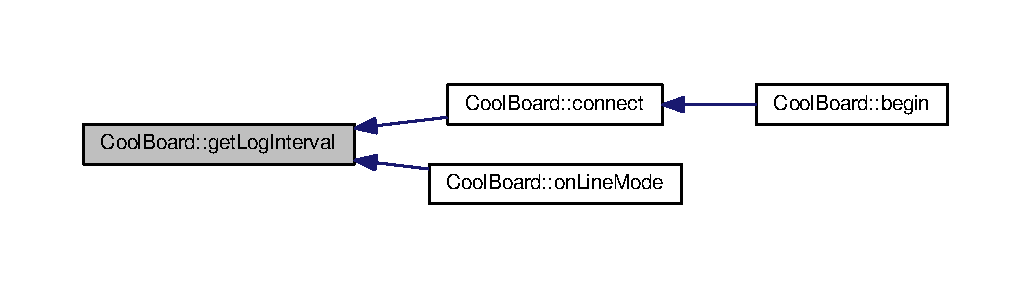
\includegraphics[width=350pt]{classCoolBoard_a7508e029f2ee17bb747ffab599285e0d_icgraph}
\end{center}
\end{figure}
\mbox{\Hypertarget{classCoolBoard_ae6b5e1274d760462290192acea4adca8}\label{classCoolBoard_ae6b5e1274d760462290192acea4adca8}} 
\index{Cool\+Board@{Cool\+Board}!off\+Line\+Mode@{off\+Line\+Mode}}
\index{off\+Line\+Mode@{off\+Line\+Mode}!Cool\+Board@{Cool\+Board}}
\subsubsection{\texorpdfstring{off\+Line\+Mode()}{offLineMode()}}
{\footnotesize\ttfamily void Cool\+Board\+::off\+Line\+Mode (\begin{DoxyParamCaption}{ }\end{DoxyParamCaption})}

Cool\+Board\+::offline\+Mode()\+: This method is provided to manage the off\+Line mode\+: -\/read sensors -\/do actions -\/save data in the file system 

Definition at line 381 of file Cool\+Board.\+cpp.



References Cool\+Board\+Led\+::blink(), cool\+Board\+Led, data, Jetpack\+::do\+Action(), Cool\+Board\+Led\+::fade(), Cool\+Board\+Led\+::fade\+In(), Cool\+Board\+Led\+::fade\+Out(), file\+System, jet\+Pack, jetpack\+Active, read\+Sensors(), Cool\+File\+System\+::save\+Sensor\+Data(), user\+Active, and user\+Data().


\begin{DoxyCode}
382 \{
383     \hyperlink{classCoolBoard_a1b1d3c684a5baa56b08486e192fd8e97}{coolBoardLed}.\hyperlink{classCoolBoardLed_af1cacbaa88db8bcf6042c1083ba41155}{fade}(51,100,50,0.5);\textcolor{comment}{//dark shade of green  }
384 \textcolor{preprocessor}{#if DEBUG == 1  }
385     
386     Serial.println( F(\textcolor{stringliteral}{"Entering off line mode "}) ); 
387     
388 \textcolor{preprocessor}{#endif}
389 
390     \textcolor{comment}{//read user data if user is active}
391     \textcolor{keywordflow}{if}(\hyperlink{classCoolBoard_a6395459131d6889a3005f79c7a35e964}{userActive})
392     \{
393 
394         \hyperlink{classCoolBoard_a1b1d3c684a5baa56b08486e192fd8e97}{coolBoardLed}.\hyperlink{classCoolBoardLed_ab778f5e7bed0ab74e3906d82110493c3}{fadeIn}(245,237,27,0.5);\textcolor{comment}{//shade of yellow}
395 
396 \textcolor{preprocessor}{    #if DEBUG == 1}
397         
398         Serial.println( F(\textcolor{stringliteral}{"User is Active"}) );
399         Serial.println( F(\textcolor{stringliteral}{"Collecting User's data ( mac,username,timeStamp )"}) );
400         Serial.println();
401 
402 \textcolor{preprocessor}{    #endif}
403 
404         \hyperlink{classCoolBoard_a1b1d3c684a5baa56b08486e192fd8e97}{coolBoardLed}.\hyperlink{classCoolBoardLed_a96e1ea13003eee34c9dbcef340404426}{blink}(245,237,27,0.5);\textcolor{comment}{//shade of yellow   }
405 
406         \textcolor{comment}{//reading user data}
407         \hyperlink{classCoolBoard_a427fb753dd8575bdf821c70a5c63d695}{data}=this->\hyperlink{classCoolBoard_ae7358fb6e623cfc81b775f5f1734909b}{userData}();\textcolor{comment}{//\{"":"","":"","",""\}}
408 
409         \textcolor{comment}{//formatting json }
410         \hyperlink{classCoolBoard_a427fb753dd8575bdf821c70a5c63d695}{data}.setCharAt( \hyperlink{classCoolBoard_a427fb753dd8575bdf821c70a5c63d695}{data}.lastIndexOf(\textcolor{charliteral}{'\}'}) , \textcolor{charliteral}{','});\textcolor{comment}{//\{"":"","":"","","",}
411         
412                 
413         \textcolor{comment}{//read sensors data}
414 \textcolor{preprocessor}{    #if DEBUG == 1}
415 
416         Serial.println( F(\textcolor{stringliteral}{"Collecting sensors data "}) );
417         Serial.println();
418 
419 \textcolor{preprocessor}{    #endif}
420 
421         \hyperlink{classCoolBoard_a427fb753dd8575bdf821c70a5c63d695}{data}+=this->\hyperlink{classCoolBoard_ad03abdce2e65f520bbf2cff0f2d083cf}{readSensors}();\textcolor{comment}{//\{"":"","":"","","",\{.......\}}
422 
423         
424 
425         \textcolor{comment}{//formatting json correctly}
426         \hyperlink{classCoolBoard_a427fb753dd8575bdf821c70a5c63d695}{data}.remove(\hyperlink{classCoolBoard_a427fb753dd8575bdf821c70a5c63d695}{data}.lastIndexOf(\textcolor{charliteral}{'\{'}), 1);\textcolor{comment}{//\{"":"","":"","","",.......\}}
427 
428         \hyperlink{classCoolBoard_a1b1d3c684a5baa56b08486e192fd8e97}{coolBoardLed}.\hyperlink{classCoolBoardLed_a93d545679237e8cc858324367149775c}{fadeOut}(245,237,27,0.5);\textcolor{comment}{//shade of yellow}
429                 
430     \}   
431     \textcolor{keywordflow}{else}
432     \{
433         \textcolor{comment}{//read sensors data}
434 \textcolor{preprocessor}{    #if DEBUG == 1}
435 
436         Serial.println( F(\textcolor{stringliteral}{"Collecting sensors data "}) );
437         Serial.println();
438 
439 \textcolor{preprocessor}{    #endif}
440 
441         \hyperlink{classCoolBoard_a1b1d3c684a5baa56b08486e192fd8e97}{coolBoardLed}.\hyperlink{classCoolBoardLed_af1cacbaa88db8bcf6042c1083ba41155}{fade}(190,100,150,0.5);\textcolor{comment}{//shade of violet        }
442 
443         \hyperlink{classCoolBoard_a427fb753dd8575bdf821c70a5c63d695}{data}=this->\hyperlink{classCoolBoard_ad03abdce2e65f520bbf2cff0f2d083cf}{readSensors}();\textcolor{comment}{//\{..,..,..\}}
444     \}
445 
446     \hyperlink{classCoolBoard_a1b1d3c684a5baa56b08486e192fd8e97}{coolBoardLed}.\hyperlink{classCoolBoardLed_af1cacbaa88db8bcf6042c1083ba41155}{fade}(51,100,50,0.5);\textcolor{comment}{//dark shade of green  }
447 
448     \textcolor{comment}{//do action}
449     \textcolor{keywordflow}{if} (\hyperlink{classCoolBoard_a9be03a913d26e558328935ca3b59a75e}{jetpackActive})
450     \{
451 
452 \textcolor{preprocessor}{    #if DEBUG == 1}
453 
454         Serial.println( F(\textcolor{stringliteral}{"jetpack is Active "}) );
455         Serial.println( F(\textcolor{stringliteral}{"jetpack doing action "}) );
456         Serial.println();
457     
458 \textcolor{preprocessor}{    #endif}
459         \hyperlink{classCoolBoard_a1b1d3c684a5baa56b08486e192fd8e97}{coolBoardLed}.\hyperlink{classCoolBoardLed_af1cacbaa88db8bcf6042c1083ba41155}{fade}(100,100,150,0.5);\textcolor{comment}{//dark shade of blue }
460     
461         \hyperlink{classCoolBoard_a30b1357881b01ccbec676856a91e48e9}{jetPack}.\hyperlink{classJetpack_a9e703197093094b963f9ad57817495b8}{doAction}( \hyperlink{classCoolBoard_a427fb753dd8575bdf821c70a5c63d695}{data}.c\_str() );
462     \}
463     
464     \hyperlink{classCoolBoard_a1b1d3c684a5baa56b08486e192fd8e97}{coolBoardLed}.\hyperlink{classCoolBoardLed_af1cacbaa88db8bcf6042c1083ba41155}{fade}(51,100,50,0.5);\textcolor{comment}{//dark shade of green  }
465     
466     \textcolor{comment}{//saving data in the file system}
467     
468     \hyperlink{classCoolBoard_a42c2586fbb13ff7f06538e9284e8538d}{fileSystem}.\hyperlink{classCoolFileSystem_afa3a4feae94871d4d3b6bebb701c2e67}{saveSensorData}( \hyperlink{classCoolBoard_a427fb753dd8575bdf821c70a5c63d695}{data}.c\_str() );
469 
470     \hyperlink{classCoolBoard_a1b1d3c684a5baa56b08486e192fd8e97}{coolBoardLed}.\hyperlink{classCoolBoardLed_a93d545679237e8cc858324367149775c}{fadeOut}(51,100,50,0.5);\textcolor{comment}{//dark shade of green    }
471 
472 \}
\end{DoxyCode}
Here is the call graph for this function\+:\nopagebreak
\begin{figure}[H]
\begin{center}
\leavevmode
\includegraphics[width=350pt]{classCoolBoard_ae6b5e1274d760462290192acea4adca8_cgraph}
\end{center}
\end{figure}
\mbox{\Hypertarget{classCoolBoard_aa0bbc4bc605e35618d18e68795c61363}\label{classCoolBoard_aa0bbc4bc605e35618d18e68795c61363}} 
\index{Cool\+Board@{Cool\+Board}!on\+Line\+Mode@{on\+Line\+Mode}}
\index{on\+Line\+Mode@{on\+Line\+Mode}!Cool\+Board@{Cool\+Board}}
\subsubsection{\texorpdfstring{on\+Line\+Mode()}{onLineMode()}}
{\footnotesize\ttfamily void Cool\+Board\+::on\+Line\+Mode (\begin{DoxyParamCaption}{ }\end{DoxyParamCaption})}

\hyperlink{classCoolBoard_aa0bbc4bc605e35618d18e68795c61363}{Cool\+Board\+::on\+Line\+Mode()}\+: This method is provided to manage the online mode\+: -\/update clock -\/read sensor -\/do actions -\/publish data -\/read answer -\/update config 

Definition at line 180 of file Cool\+Board.\+cpp.



References answer, Cool\+Board\+Led\+::blink(), cool\+Board\+Led, data, Jetpack\+::do\+Action(), Cool\+Board\+Led\+::fade(), Cool\+Board\+Led\+::fade\+In(), Cool\+Board\+Led\+::fade\+Out(), file\+System, get\+Log\+Interval(), Cool\+File\+System\+::get\+Sensor\+Saved\+Data(), Cool\+File\+System\+::is\+Data\+Saved(), jet\+Pack, jetpack\+Active, mqtt, Cool\+M\+Q\+T\+T\+::mqtt\+Loop(), Cool\+M\+Q\+T\+T\+::publish(), Cool\+M\+Q\+T\+T\+::read(), read\+Sensors(), rtc, sleep(), sleep\+Active, Cool\+Board\+Led\+::strobe(), Cool\+Time\+::update(), update(), user\+Active, and user\+Data().


\begin{DoxyCode}
181 \{
182 
183     \hyperlink{classCoolBoard_a1b1d3c684a5baa56b08486e192fd8e97}{coolBoardLed}.\hyperlink{classCoolBoardLed_ab778f5e7bed0ab74e3906d82110493c3}{fadeIn}(128,255,50,0.5);\textcolor{comment}{//shade of green}
184 
185 \textcolor{preprocessor}{#if DEBUG == 1}
186 
187     Serial.println( F(\textcolor{stringliteral}{"Entering CoolBoard.onLineMode() "}) );
188     Serial.println();
189 
190 \textcolor{preprocessor}{#endif}
191 
192     \hyperlink{classCoolBoard_a427fb753dd8575bdf821c70a5c63d695}{data}=\textcolor{stringliteral}{""};
193     \hyperlink{classCoolBoard_a7b835fafd449e5282f7f91d787a2dc15}{answer}=\textcolor{stringliteral}{""};
194 
195     \textcolor{comment}{//send saved data if any}
196     \textcolor{keywordflow}{if}(\hyperlink{classCoolBoard_a42c2586fbb13ff7f06538e9284e8538d}{fileSystem}.\hyperlink{classCoolFileSystem_a5a7eaeea7a9fbf8aaef651d862fa3b5b}{isDataSaved}())
197     \{
198 
199         \hyperlink{classCoolBoard_a1b1d3c684a5baa56b08486e192fd8e97}{coolBoardLed}.\hyperlink{classCoolBoardLed_ab778f5e7bed0ab74e3906d82110493c3}{fadeIn}(128,128,255,0.5);\textcolor{comment}{//shade of blue}
200 
201 \textcolor{preprocessor}{    #if DEBUG == 1}
202 
203         Serial.println( F(\textcolor{stringliteral}{"There is data saved on the File System"}) );
204         Serial.println( F(\textcolor{stringliteral}{"Sending saved data over MQTT "}) );
205         Serial.println();
206     
207 \textcolor{preprocessor}{    #endif  }
208         \hyperlink{classCoolBoard_a1b1d3c684a5baa56b08486e192fd8e97}{coolBoardLed}.\hyperlink{classCoolBoardLed_ad5f0de4c628cbfbf49896042831c64ad}{strobe}(128,128,255,0.5);\textcolor{comment}{//shade of blue }
209 
210         \hyperlink{classCoolBoard_a2399f44d7c23c1149a335cb3b46d90f1}{mqtt}.\hyperlink{classCoolMQTT_ace977b3e90ab14b1199fe5c4fb0a13ec}{publish}(\textcolor{stringliteral}{"sending saved data"});
211         \hyperlink{classCoolBoard_a2399f44d7c23c1149a335cb3b46d90f1}{mqtt}.\hyperlink{classCoolMQTT_aa5eaae967b562b62cbcf2b8d81f6e5d5}{mqttLoop}();
212 
213         \hyperlink{classCoolBoard_a427fb753dd8575bdf821c70a5c63d695}{data}+=\hyperlink{classCoolBoard_a42c2586fbb13ff7f06538e9284e8538d}{fileSystem}.\hyperlink{classCoolFileSystem_a5c58bca3735c0ed3efb268d70ef998ef}{getSensorSavedData}();\textcolor{comment}{//\{..,..,..\}}
214 
215         \textcolor{comment}{//formatting data:}
216         String jsonData = \textcolor{stringliteral}{"\{\(\backslash\)"state\(\backslash\)":\{\(\backslash\)"reported\(\backslash\)":"};
217         jsonData += \hyperlink{classCoolBoard_a427fb753dd8575bdf821c70a5c63d695}{data}; \textcolor{comment}{// \{"state":\{"reported":\{..,..,..,..,..,..,..,..\}}
218         jsonData += \textcolor{stringliteral}{" \} \}"}; \textcolor{comment}{// \{"state":\{"reported":\{..,..,..,..,..,..,..,..\}  \} \}}
219         
220         \hyperlink{classCoolBoard_a1b1d3c684a5baa56b08486e192fd8e97}{coolBoardLed}.\hyperlink{classCoolBoardLed_ad5f0de4c628cbfbf49896042831c64ad}{strobe}(128,128,255,0.5);\textcolor{comment}{//shade of blue}
221         
222         \hyperlink{classCoolBoard_a2399f44d7c23c1149a335cb3b46d90f1}{mqtt}.\hyperlink{classCoolMQTT_ace977b3e90ab14b1199fe5c4fb0a13ec}{publish}( \hyperlink{classCoolBoard_a427fb753dd8575bdf821c70a5c63d695}{data}.c\_str() );
223         \hyperlink{classCoolBoard_a2399f44d7c23c1149a335cb3b46d90f1}{mqtt}.\hyperlink{classCoolMQTT_aa5eaae967b562b62cbcf2b8d81f6e5d5}{mqttLoop}();
224         
225         \hyperlink{classCoolBoard_a1b1d3c684a5baa56b08486e192fd8e97}{coolBoardLed}.\hyperlink{classCoolBoardLed_a93d545679237e8cc858324367149775c}{fadeOut}(128,128,255,0.5);\textcolor{comment}{//shade of blue        }
226     
227 \textcolor{preprocessor}{    #if DEBUG == 1}
228 
229         Serial.println( F(\textcolor{stringliteral}{"Saved data sent "}) );
230         Serial.println();
231     
232 \textcolor{preprocessor}{    #endif}
233 
234     \}
235 
236     \hyperlink{classCoolBoard_a1b1d3c684a5baa56b08486e192fd8e97}{coolBoardLed}.\hyperlink{classCoolBoardLed_a96e1ea13003eee34c9dbcef340404426}{blink}(128,255,50,0.5);\textcolor{comment}{//shade of green}
237 
238     \textcolor{comment}{//clock update}
239     \hyperlink{classCoolBoard_a50d2a6716879d64a85f3c6b44ad63275}{rtc}.\hyperlink{classCoolTime_aae601f795452cfa48d9fb337aed483a8}{update}();
240 
241     \textcolor{comment}{//read user data if user is active}
242     \textcolor{keywordflow}{if}(\hyperlink{classCoolBoard_a6395459131d6889a3005f79c7a35e964}{userActive})
243     \{
244         \hyperlink{classCoolBoard_a1b1d3c684a5baa56b08486e192fd8e97}{coolBoardLed}.\hyperlink{classCoolBoardLed_ab778f5e7bed0ab74e3906d82110493c3}{fadeIn}(245,237,27,0.5);\textcolor{comment}{//shade of yellow}
245     
246 \textcolor{preprocessor}{    #if DEBUG == 1}
247 
248         Serial.println( F(\textcolor{stringliteral}{"User is Active"}) );
249         Serial.println( F(\textcolor{stringliteral}{"Collecting User's data ( mac,username,timeStamp )"}) );
250         Serial.println();
251     
252 \textcolor{preprocessor}{    #endif  }
253         \hyperlink{classCoolBoard_a1b1d3c684a5baa56b08486e192fd8e97}{coolBoardLed}.\hyperlink{classCoolBoardLed_a96e1ea13003eee34c9dbcef340404426}{blink}(245,237,27,0.5);\textcolor{comment}{//shade of yellow   }
254 
255         \textcolor{comment}{//reading user data}
256         \hyperlink{classCoolBoard_a427fb753dd8575bdf821c70a5c63d695}{data}=this->\hyperlink{classCoolBoard_ae7358fb6e623cfc81b775f5f1734909b}{userData}();\textcolor{comment}{//\{"":"","":"","",""\}}
257 
258         \textcolor{comment}{//formatting json }
259         \hyperlink{classCoolBoard_a427fb753dd8575bdf821c70a5c63d695}{data}.setCharAt( \hyperlink{classCoolBoard_a427fb753dd8575bdf821c70a5c63d695}{data}.lastIndexOf(\textcolor{charliteral}{'\}'}) , \textcolor{charliteral}{','});\textcolor{comment}{//\{"":"","":"","","",}
260                 
261         \textcolor{comment}{//read sensors data}
262 \textcolor{preprocessor}{    #if DEBUG == 1}
263 
264         Serial.println( F(\textcolor{stringliteral}{"Collecting sensors data "}) );
265         Serial.println();
266     
267 \textcolor{preprocessor}{    #endif}
268 
269         \hyperlink{classCoolBoard_a427fb753dd8575bdf821c70a5c63d695}{data}+=this->\hyperlink{classCoolBoard_ad03abdce2e65f520bbf2cff0f2d083cf}{readSensors}();\textcolor{comment}{//\{"":"","":"","","",\{.......\}     }
270 
271         \textcolor{comment}{//formatting json correctly}
272         \hyperlink{classCoolBoard_a427fb753dd8575bdf821c70a5c63d695}{data}.remove(\hyperlink{classCoolBoard_a427fb753dd8575bdf821c70a5c63d695}{data}.lastIndexOf(\textcolor{charliteral}{'\{'}), 1);\textcolor{comment}{//\{"":"","":"","","",.......\}}
273         
274         \hyperlink{classCoolBoard_a1b1d3c684a5baa56b08486e192fd8e97}{coolBoardLed}.\hyperlink{classCoolBoardLed_a93d545679237e8cc858324367149775c}{fadeOut}(245,237,27,0.5);\textcolor{comment}{//shade of yellow}
275                 
276     \}   
277     \textcolor{keywordflow}{else}
278     \{
279         \textcolor{comment}{//read sensors data}
280 \textcolor{preprocessor}{    #if DEBUG == 1}
281 
282         Serial.println( F(\textcolor{stringliteral}{"Collecting sensors data "}) );
283         Serial.println();
284     
285 \textcolor{preprocessor}{    #endif}
286         \hyperlink{classCoolBoard_a1b1d3c684a5baa56b08486e192fd8e97}{coolBoardLed}.\hyperlink{classCoolBoardLed_af1cacbaa88db8bcf6042c1083ba41155}{fade}(190,100,150,0.5);\textcolor{comment}{//shade of violet        }
287         \hyperlink{classCoolBoard_a427fb753dd8575bdf821c70a5c63d695}{data}=this->\hyperlink{classCoolBoard_ad03abdce2e65f520bbf2cff0f2d083cf}{readSensors}();\textcolor{comment}{//\{..,..,..\}}
288     \}
289     
290     \textcolor{comment}{//do action}
291     \textcolor{keywordflow}{if} (\hyperlink{classCoolBoard_a9be03a913d26e558328935ca3b59a75e}{jetpackActive})
292     \{
293     
294 \textcolor{preprocessor}{    #if DEBUG ==1}
295 
296         Serial.println( F(\textcolor{stringliteral}{"jetpack is Active "}) );
297         Serial.println( F(\textcolor{stringliteral}{"jetpack doing action "}) );
298         Serial.println();
299 
300 \textcolor{preprocessor}{    #endif}
301         \hyperlink{classCoolBoard_a1b1d3c684a5baa56b08486e192fd8e97}{coolBoardLed}.\hyperlink{classCoolBoardLed_af1cacbaa88db8bcf6042c1083ba41155}{fade}(100,100,150,0.5);\textcolor{comment}{//dark shade of blue     }
302         \hyperlink{classCoolBoard_a30b1357881b01ccbec676856a91e48e9}{jetPack}.\hyperlink{classJetpack_a9e703197093094b963f9ad57817495b8}{doAction}(\hyperlink{classCoolBoard_a427fb753dd8575bdf821c70a5c63d695}{data}.c\_str());
303     \}
304     
305     \hyperlink{classCoolBoard_a1b1d3c684a5baa56b08486e192fd8e97}{coolBoardLed}.\hyperlink{classCoolBoardLed_ab778f5e7bed0ab74e3906d82110493c3}{fadeIn}(128,255,50,0.5);\textcolor{comment}{//shade of green}
306 
307     \textcolor{comment}{//formatting data:}
308     String jsonData = \textcolor{stringliteral}{"\{\(\backslash\)"state\(\backslash\)":\{\(\backslash\)"reported\(\backslash\)":"};
309     jsonData += \hyperlink{classCoolBoard_a427fb753dd8575bdf821c70a5c63d695}{data}; \textcolor{comment}{// \{"state":\{"reported":\{..,..,..,..,..,..,..,..\}}
310     jsonData += \textcolor{stringliteral}{" \} \}"}; \textcolor{comment}{// \{"state":\{"reported":\{..,..,..,..,..,..,..,..\}  \} \}}
311     
312     \textcolor{comment}{//mqtt client loop to allow data handling}
313     \hyperlink{classCoolBoard_a2399f44d7c23c1149a335cb3b46d90f1}{mqtt}.\hyperlink{classCoolMQTT_aa5eaae967b562b62cbcf2b8d81f6e5d5}{mqttLoop}();
314 
315     \hyperlink{classCoolBoard_a1b1d3c684a5baa56b08486e192fd8e97}{coolBoardLed}.\hyperlink{classCoolBoardLed_a96e1ea13003eee34c9dbcef340404426}{blink}(128,255,50,0.5);\textcolor{comment}{//shade of green    }
316 
317     \textcolor{comment}{//read mqtt answer}
318     \hyperlink{classCoolBoard_a7b835fafd449e5282f7f91d787a2dc15}{answer} = \hyperlink{classCoolBoard_a2399f44d7c23c1149a335cb3b46d90f1}{mqtt}.\hyperlink{classCoolMQTT_ae3c18f6ae9723746d32765f1c8f176ca}{read}();
319 
320 \textcolor{preprocessor}{#if DEBUG == 1 }
321 
322     Serial.println( F(\textcolor{stringliteral}{"checking if there's an MQTT message "})  );
323     Serial.println( F(\textcolor{stringliteral}{"answer is : "}) );    
324     Serial.println(\hyperlink{classCoolBoard_a7b835fafd449e5282f7f91d787a2dc15}{answer});   
325     Serial.println();
326 
327 \textcolor{preprocessor}{#endif  }
328 
329     \hyperlink{classCoolBoard_a1b1d3c684a5baa56b08486e192fd8e97}{coolBoardLed}.\hyperlink{classCoolBoardLed_a93d545679237e8cc858324367149775c}{fadeOut}(128,255,50,0.5);\textcolor{comment}{//shade of green    }
330 
331     \textcolor{comment}{//check if the configuration needs update }
332     \textcolor{comment}{//and update it if needed }
333     \textcolor{keyword}{this} -> \hyperlink{classCoolBoard_a8612756d3f73198cdde857a66f0fe690}{update}(\hyperlink{classCoolBoard_a7b835fafd449e5282f7f91d787a2dc15}{answer}.c\_str());
334     
335     \hyperlink{classCoolBoard_a1b1d3c684a5baa56b08486e192fd8e97}{coolBoardLed}.\hyperlink{classCoolBoardLed_ab778f5e7bed0ab74e3906d82110493c3}{fadeIn}(128,255,50,0.5);\textcolor{comment}{//shade of green  }
336 
337     \textcolor{comment}{//publishing data   }
338     \textcolor{keywordflow}{if}( this->\hyperlink{classCoolBoard_a0a51b2287139f66c738101fb53139230}{sleepActive}==0)    
339     \{   
340         \hyperlink{classCoolBoard_a1b1d3c684a5baa56b08486e192fd8e97}{coolBoardLed}.\hyperlink{classCoolBoardLed_ad5f0de4c628cbfbf49896042831c64ad}{strobe}(255,0,230,0.5);\textcolor{comment}{//shade of pink}
341         
342         \textcolor{comment}{//logInterval in seconds}
343         \hyperlink{classCoolBoard_a2399f44d7c23c1149a335cb3b46d90f1}{mqtt}.\hyperlink{classCoolMQTT_ace977b3e90ab14b1199fe5c4fb0a13ec}{publish}( jsonData.c\_str(), this->\hyperlink{classCoolBoard_a7508e029f2ee17bb747ffab599285e0d}{getLogInterval}() );
344         \hyperlink{classCoolBoard_a2399f44d7c23c1149a335cb3b46d90f1}{mqtt}.\hyperlink{classCoolMQTT_aa5eaae967b562b62cbcf2b8d81f6e5d5}{mqttLoop}();
345     
346     \}
347     \textcolor{keywordflow}{else}
348     \{
349         \hyperlink{classCoolBoard_a1b1d3c684a5baa56b08486e192fd8e97}{coolBoardLed}.\hyperlink{classCoolBoardLed_ad5f0de4c628cbfbf49896042831c64ad}{strobe}(230,255,0,0.5);\textcolor{comment}{//shade of yellow  }
350 
351         \hyperlink{classCoolBoard_a2399f44d7c23c1149a335cb3b46d90f1}{mqtt}.\hyperlink{classCoolMQTT_ace977b3e90ab14b1199fe5c4fb0a13ec}{publish}(jsonData.c\_str());      
352         \hyperlink{classCoolBoard_a2399f44d7c23c1149a335cb3b46d90f1}{mqtt}.\hyperlink{classCoolMQTT_aa5eaae967b562b62cbcf2b8d81f6e5d5}{mqttLoop}();
353         \hyperlink{classCoolBoard_a7b835fafd449e5282f7f91d787a2dc15}{answer} = \hyperlink{classCoolBoard_a2399f44d7c23c1149a335cb3b46d90f1}{mqtt}.\hyperlink{classCoolMQTT_ae3c18f6ae9723746d32765f1c8f176ca}{read}();
354         \textcolor{keyword}{this} ->update(\hyperlink{classCoolBoard_a7b835fafd449e5282f7f91d787a2dc15}{answer}.c\_str());
355 
356         \textcolor{comment}{//logInterval in seconds}
357         this->\hyperlink{classCoolBoard_a069952cdcb2e7f68518aa429eceadb6e}{sleep}( this->\hyperlink{classCoolBoard_a7508e029f2ee17bb747ffab599285e0d}{getLogInterval}() ) ;
358     \}
359 
360     \hyperlink{classCoolBoard_a1b1d3c684a5baa56b08486e192fd8e97}{coolBoardLed}.\hyperlink{classCoolBoardLed_a93d545679237e8cc858324367149775c}{fadeOut}(128,255,50,0.5);\textcolor{comment}{//shade of green        }
361 
362     \hyperlink{classCoolBoard_a2399f44d7c23c1149a335cb3b46d90f1}{mqtt}.\hyperlink{classCoolMQTT_aa5eaae967b562b62cbcf2b8d81f6e5d5}{mqttLoop}();
363 
364     \textcolor{comment}{//read mqtt answer}
365     \hyperlink{classCoolBoard_a7b835fafd449e5282f7f91d787a2dc15}{answer} = \hyperlink{classCoolBoard_a2399f44d7c23c1149a335cb3b46d90f1}{mqtt}.\hyperlink{classCoolMQTT_ae3c18f6ae9723746d32765f1c8f176ca}{read}();
366     \textcolor{keyword}{this} -> \hyperlink{classCoolBoard_a8612756d3f73198cdde857a66f0fe690}{update}(\hyperlink{classCoolBoard_a7b835fafd449e5282f7f91d787a2dc15}{answer}.c\_str()); 
367 
368     \hyperlink{classCoolBoard_a1b1d3c684a5baa56b08486e192fd8e97}{coolBoardLed}.\hyperlink{classCoolBoardLed_a96e1ea13003eee34c9dbcef340404426}{blink}(128,255,50,0.5);\textcolor{comment}{//shade of green    }
369 
370 
371 \}
\end{DoxyCode}
Here is the call graph for this function\+:\nopagebreak
\begin{figure}[H]
\begin{center}
\leavevmode
\includegraphics[width=350pt]{classCoolBoard_aa0bbc4bc605e35618d18e68795c61363_cgraph}
\end{center}
\end{figure}
\mbox{\Hypertarget{classCoolBoard_a486507b8f0981d3cc671ed31c2145755}\label{classCoolBoard_a486507b8f0981d3cc671ed31c2145755}} 
\index{Cool\+Board@{Cool\+Board}!print\+Conf@{print\+Conf}}
\index{print\+Conf@{print\+Conf}!Cool\+Board@{Cool\+Board}}
\subsubsection{\texorpdfstring{print\+Conf()}{printConf()}}
{\footnotesize\ttfamily void Cool\+Board\+::print\+Conf (\begin{DoxyParamCaption}{ }\end{DoxyParamCaption})}

\hyperlink{classCoolBoard_a486507b8f0981d3cc671ed31c2145755}{Cool\+Board\+::print\+Conf()}\+: This method is provided to print the configuration to the Serial Monitor. 

Definition at line 673 of file Cool\+Board.\+cpp.



References external\+Sensors\+Active, irene\+Active, jetpack\+Active, log\+Interval, server\+Time\+Out, sleep\+Active, and user\+Active.


\begin{DoxyCode}
674 \{
675 
676 \textcolor{preprocessor}{#if DEBUG == 1}
677     
678     Serial.println( F(\textcolor{stringliteral}{"Entering CoolBoard.printConf() "}) );
679     Serial.println();
680 
681 \textcolor{preprocessor}{#endif}
682 
683     Serial.println(\textcolor{stringliteral}{"Printing Cool Board Configuration "});
684     Serial.print(\textcolor{stringliteral}{"log interval      : "});
685     Serial.println(this->\hyperlink{classCoolBoard_a84bc94413b64973e4aba8c467c97006c}{logInterval});
686 
687     Serial.print(\textcolor{stringliteral}{"irene active      : "});
688     Serial.println(this->\hyperlink{classCoolBoard_a9c3f7ac625481ee2ae802a25d97a4ae0}{ireneActive});
689 
690     Serial.print(\textcolor{stringliteral}{"jetpack active        : "});
691     Serial.println(this->\hyperlink{classCoolBoard_a9be03a913d26e558328935ca3b59a75e}{jetpackActive});
692 
693     Serial.print(\textcolor{stringliteral}{"external sensors active   : "});
694     Serial.println(this->\hyperlink{classCoolBoard_a638b00b76aeb819ecfd4c10b8cdd7bb7}{externalSensorsActive});
695 
696     Serial.print(\textcolor{stringliteral}{"access point timeOut  : "});
697     Serial.println(this->\hyperlink{classCoolBoard_a7a8d8d3d316220cdd049cd63c1aa8fe6}{serverTimeOut});
698 
699     Serial.print(\textcolor{stringliteral}{"sleept active         : "});
700     Serial.println(this->\hyperlink{classCoolBoard_a0a51b2287139f66c738101fb53139230}{sleepActive});
701 
702     Serial.print(\textcolor{stringliteral}{"user active       : "});
703     Serial.println(this->\hyperlink{classCoolBoard_a6395459131d6889a3005f79c7a35e964}{userActive});
704 
705     Serial.println();
706 
707 
708 
709 
710 \}
\end{DoxyCode}
\mbox{\Hypertarget{classCoolBoard_ad03abdce2e65f520bbf2cff0f2d083cf}\label{classCoolBoard_ad03abdce2e65f520bbf2cff0f2d083cf}} 
\index{Cool\+Board@{Cool\+Board}!read\+Sensors@{read\+Sensors}}
\index{read\+Sensors@{read\+Sensors}!Cool\+Board@{Cool\+Board}}
\subsubsection{\texorpdfstring{read\+Sensors()}{readSensors()}}
{\footnotesize\ttfamily String Cool\+Board\+::read\+Sensors (\begin{DoxyParamCaption}{ }\end{DoxyParamCaption})}

\hyperlink{classCoolBoard_ad03abdce2e65f520bbf2cff0f2d083cf}{Cool\+Board\+::read\+Sensors()}\+: This method is provided to read and format all the sensors data in a single json.

\begin{DoxyReturn}{Returns}
json string of all the sensors read. 
\end{DoxyReturn}


Definition at line 888 of file Cool\+Board.\+cpp.



References cool\+Board\+Led, cool\+Board\+Sensors, external\+Sensors, external\+Sensors\+Active, Cool\+Board\+Led\+::fade\+In(), Cool\+Board\+Led\+::fade\+Out(), Cool\+Time\+::get\+Time\+Date(), irene3000, irene\+Active, External\+Sensors\+::read(), Cool\+Board\+Sensors\+::read(), Irene3000\+::read(), rtc, and Cool\+Board\+Led\+::strobe().



Referenced by off\+Line\+Mode(), and on\+Line\+Mode().


\begin{DoxyCode}
889 \{
890 
891     \hyperlink{classCoolBoard_a1b1d3c684a5baa56b08486e192fd8e97}{coolBoardLed}.\hyperlink{classCoolBoardLed_ab778f5e7bed0ab74e3906d82110493c3}{fadeIn}(128,255,0,0.5);\textcolor{comment}{//light shade of green}
892                 
893 \textcolor{preprocessor}{#if DEBUG == 1}
894 
895     Serial.println( F(\textcolor{stringliteral}{"Entering CoolBoard.readSensors()"}) );
896     Serial.println();
897 
898 \textcolor{preprocessor}{#endif}
899     \hyperlink{classCoolBoard_a1b1d3c684a5baa56b08486e192fd8e97}{coolBoardLed}.\hyperlink{classCoolBoardLed_ad5f0de4c628cbfbf49896042831c64ad}{strobe}(128,255,0,0.5);\textcolor{comment}{//light shade of green}
900 
901     String sensorsData;
902 
903     sensorsData = \hyperlink{classCoolBoard_af102be5288bd7f7a8e59b13f86e26a00}{coolBoardSensors}.\hyperlink{classCoolBoardSensors_a91badb2539d91fda8679f2a597874c48}{read}(); \textcolor{comment}{// \{..,..,..\}}
904     
905     \textcolor{keywordflow}{if} (\hyperlink{classCoolBoard_a638b00b76aeb819ecfd4c10b8cdd7bb7}{externalSensorsActive})
906     \{
907         sensorsData += \hyperlink{classCoolBoard_a09e26264839c65873eb56af476eff6b2}{externalSensors}.\hyperlink{classExternalSensors_a53177b81eca3be89508b5511ddcd00fc}{read}(); \textcolor{comment}{// \{..,..,..\}\{..,..\}}
908 
909         sensorsData.setCharAt(sensorsData.lastIndexOf(\textcolor{charliteral}{'\}'}), \textcolor{charliteral}{','}); \textcolor{comment}{// \{..,..,..\}\{..,..,}
910         sensorsData.setCharAt(sensorsData.lastIndexOf(\textcolor{charliteral}{'\{'}), \textcolor{charliteral}{','}); \textcolor{comment}{// \{..,..,..\},..,..,}
911         sensorsData.remove(sensorsData.lastIndexOf(\textcolor{charliteral}{'\}'}), 1); \textcolor{comment}{// \{..,..,..,..,..,}
912         sensorsData.setCharAt(sensorsData.lastIndexOf(\textcolor{charliteral}{','}), \textcolor{charliteral}{'\}'}); \textcolor{comment}{// \{..,..,..,..,..\}}
913 
914     \}
915     \textcolor{keywordflow}{if} (\hyperlink{classCoolBoard_a9c3f7ac625481ee2ae802a25d97a4ae0}{ireneActive})
916     \{
917         sensorsData += \hyperlink{classCoolBoard_ad103718ce316006c4695b8eb312eaf11}{irene3000}.\hyperlink{classIrene3000_a852a170feea994ea1df01c6b245b5d9a}{read}(); \textcolor{comment}{// \{..,..,..,..,..\}\{..,..,..\}}
918 
919         sensorsData.setCharAt(sensorsData.lastIndexOf(\textcolor{charliteral}{'\}'}), \textcolor{charliteral}{','}); \textcolor{comment}{// \{..,..,..,..,..\}\{..,..,..,}
920         sensorsData.setCharAt(sensorsData.lastIndexOf(\textcolor{charliteral}{'\{'}), \textcolor{charliteral}{','}); \textcolor{comment}{// \{..,..,..,..,..\},..,..,..,}
921         sensorsData.remove(sensorsData.lastIndexOf(\textcolor{charliteral}{'\}'}), 1); \textcolor{comment}{// \{..,..,..,..,..,..,..,..,}
922         sensorsData.setCharAt(sensorsData.lastIndexOf(\textcolor{charliteral}{','}), \textcolor{charliteral}{'\}'}); \textcolor{comment}{// \{..,..,..,..,..,..,..,..\}      }
923         
924         
925     \}
926 
927     \textcolor{comment}{//getting Hour:}
928     tmElements\_t tm;
929     tm=\hyperlink{classCoolBoard_a50d2a6716879d64a85f3c6b44ad63275}{rtc}.\hyperlink{classCoolTime_a7a7501c5ca77dd1248bea704c44f986c}{getTimeDate}();
930     
931     \textcolor{comment}{//adding Hour}
932     sensorsData.remove(sensorsData.lastIndexOf(\textcolor{charliteral}{'\}'}), 1); \textcolor{comment}{// \{..,..,..,..,..,..,..,..,   }
933     sensorsData+=\textcolor{stringliteral}{",\(\backslash\)"hour\(\backslash\)":"};  
934     sensorsData+=tm.Hour;
935     sensorsData+=\textcolor{stringliteral}{"\}"};
936     
937 \textcolor{preprocessor}{#if DEBUG == 1}
938     Serial.println();
939     Serial.println( F(\textcolor{stringliteral}{"sensors data is "}) );
940     Serial.println(sensorsData);
941     Serial.println();
942 
943 \textcolor{preprocessor}{#endif}
944     \hyperlink{classCoolBoard_a1b1d3c684a5baa56b08486e192fd8e97}{coolBoardLed}.\hyperlink{classCoolBoardLed_a93d545679237e8cc858324367149775c}{fadeOut}(128,255,0,0.5);\textcolor{comment}{//light shade of green}
945 
946     \textcolor{keywordflow}{return}(sensorsData);
947 
948 \}
\end{DoxyCode}
Here is the call graph for this function\+:\nopagebreak
\begin{figure}[H]
\begin{center}
\leavevmode
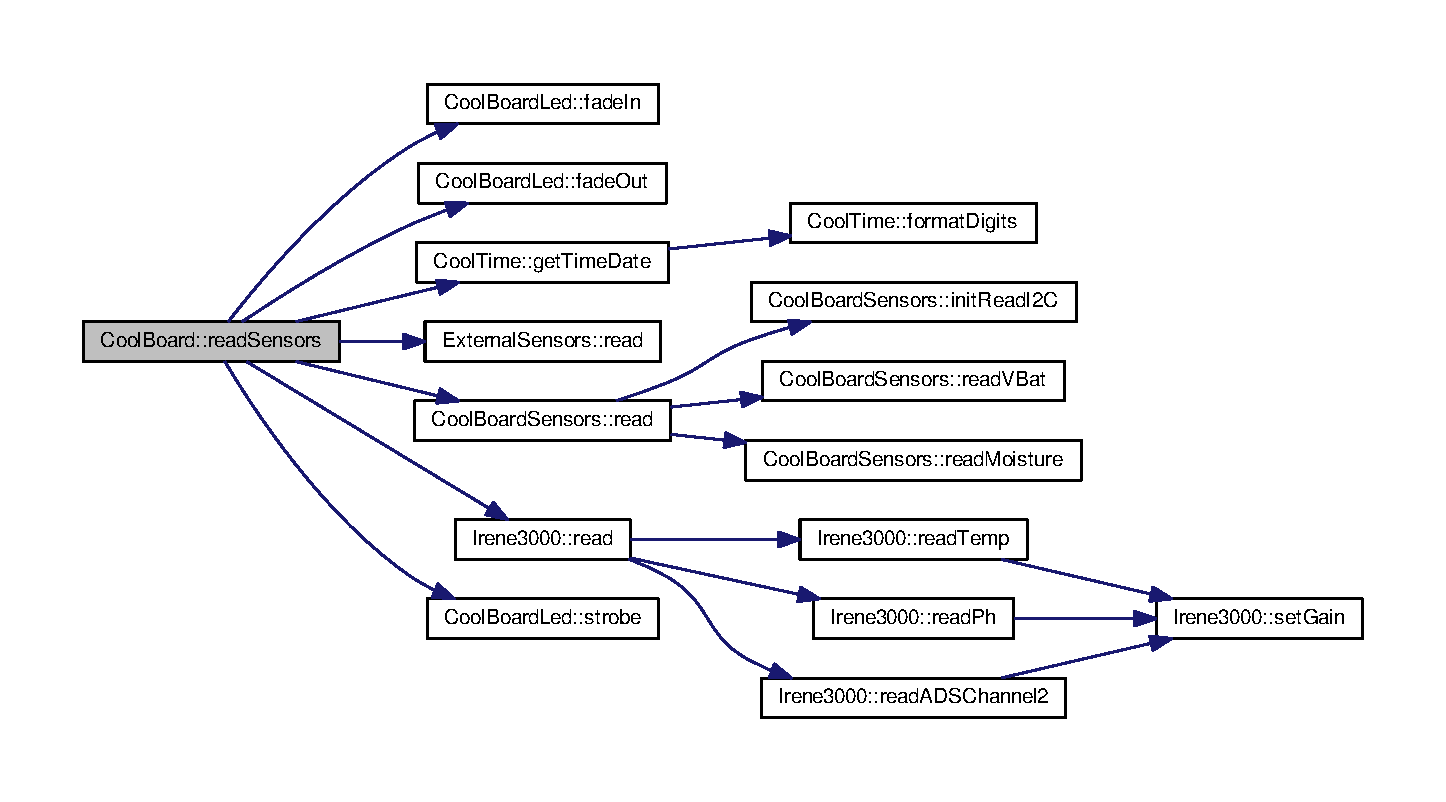
\includegraphics[width=350pt]{classCoolBoard_ad03abdce2e65f520bbf2cff0f2d083cf_cgraph}
\end{center}
\end{figure}
Here is the caller graph for this function\+:\nopagebreak
\begin{figure}[H]
\begin{center}
\leavevmode
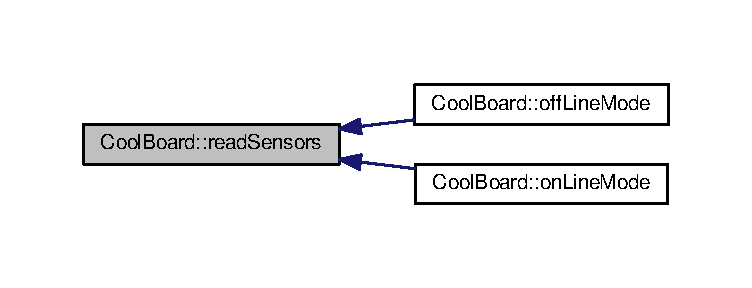
\includegraphics[width=350pt]{classCoolBoard_ad03abdce2e65f520bbf2cff0f2d083cf_icgraph}
\end{center}
\end{figure}
\mbox{\Hypertarget{classCoolBoard_a069952cdcb2e7f68518aa429eceadb6e}\label{classCoolBoard_a069952cdcb2e7f68518aa429eceadb6e}} 
\index{Cool\+Board@{Cool\+Board}!sleep@{sleep}}
\index{sleep@{sleep}!Cool\+Board@{Cool\+Board}}
\subsubsection{\texorpdfstring{sleep()}{sleep()}}
{\footnotesize\ttfamily void Cool\+Board\+::sleep (\begin{DoxyParamCaption}\item[{unsigned long}]{interval }\end{DoxyParamCaption})}

Cool\+Board\+::sleep(int interval)\+: This method is provided to allow the board to enter deep\+Sleep mode for a period of time equal to interval in s 

Definition at line 1004 of file Cool\+Board.\+cpp.



Referenced by on\+Line\+Mode().


\begin{DoxyCode}
1005 \{
1006 
1007 \textcolor{preprocessor}{#if DEBUG == 1}
1008 
1009     Serial.println( F(\textcolor{stringliteral}{"Entering CoolBoard.sleep() "}) );
1010     Serial.print( F(\textcolor{stringliteral}{"going to sleep for "}) );
1011     Serial.print(interval);
1012     Serial.println(F(\textcolor{stringliteral}{"s"}) );
1013     Serial.println();
1014 
1015 \textcolor{preprocessor}{#endif}
1016     \textcolor{comment}{//interval is in seconds , interval*1000*1000 in µS}
1017     ESP.deepSleep ( ( interval * 1000 * 1000 ), WAKE\_RF\_DEFAULT) ;
1018 \}
\end{DoxyCode}
Here is the caller graph for this function\+:\nopagebreak
\begin{figure}[H]
\begin{center}
\leavevmode
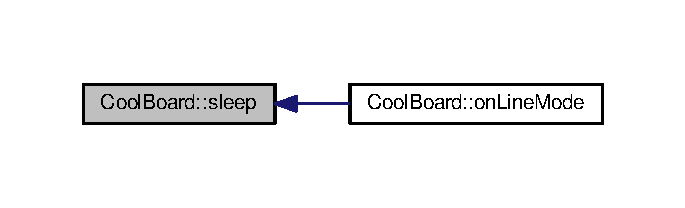
\includegraphics[width=329pt]{classCoolBoard_a069952cdcb2e7f68518aa429eceadb6e_icgraph}
\end{center}
\end{figure}
\mbox{\Hypertarget{classCoolBoard_a8612756d3f73198cdde857a66f0fe690}\label{classCoolBoard_a8612756d3f73198cdde857a66f0fe690}} 
\index{Cool\+Board@{Cool\+Board}!update@{update}}
\index{update@{update}!Cool\+Board@{Cool\+Board}}
\subsubsection{\texorpdfstring{update()}{update()}}
{\footnotesize\ttfamily void Cool\+Board\+::update (\begin{DoxyParamCaption}\item[{const char $\ast$}]{answer }\end{DoxyParamCaption})}

Cool\+Board\+::update(mqtt answer)\+: This method is provided to handle the configuration update of the different parts 

Definition at line 717 of file Cool\+Board.\+cpp.



References cool\+Board\+Led, Cool\+Board\+Led\+::fade\+In(), Cool\+Board\+Led\+::fade\+Out(), file\+System, mqtt, Cool\+M\+Q\+T\+T\+::mqtt\+Loop(), Cool\+M\+Q\+T\+T\+::publish(), Cool\+Board\+Led\+::strobe(), and Cool\+File\+System\+::update\+Config\+Files().



Referenced by on\+Line\+Mode().


\begin{DoxyCode}
718 \{
719     \hyperlink{classCoolBoard_a1b1d3c684a5baa56b08486e192fd8e97}{coolBoardLed}.\hyperlink{classCoolBoardLed_ab778f5e7bed0ab74e3906d82110493c3}{fadeIn}(153,76,0,0.5);\textcolor{comment}{//shade of brown        }
720 
721 \textcolor{preprocessor}{#if DEBUG == 1}
722 
723     Serial.println( F(\textcolor{stringliteral}{"Entering CoolBoard.update() "}) );
724     Serial.println();
725     Serial.println( F(\textcolor{stringliteral}{"message is : "}) );
726     Serial.println(\hyperlink{classCoolBoard_a7b835fafd449e5282f7f91d787a2dc15}{answer});
727     Serial.println();
728 
729 \textcolor{preprocessor}{#endif}
730 
731     DynamicJsonBuffer jsonBuffer;
732     JsonObject & root = jsonBuffer.parseObject(\hyperlink{classCoolBoard_a7b835fafd449e5282f7f91d787a2dc15}{answer});
733     JsonObject & stateDesired = root[\textcolor{stringliteral}{"state"}];
734 
735 \textcolor{preprocessor}{#if DEBUG == 1}
736 
737     Serial.println( F(\textcolor{stringliteral}{"root json : "}) );
738     root.printTo(Serial);
739     Serial.println();
740 
741     Serial.println(F(\textcolor{stringliteral}{"stateDesired json : "}));
742     stateDesired.printTo(Serial);
743     Serial.println();
744     
745     Serial.print(F(\textcolor{stringliteral}{"jsonBuffer size : "}));
746     Serial.println(jsonBuffer.size());
747 
748 \textcolor{preprocessor}{#endif}
749 
750     \textcolor{keywordflow}{if} (stateDesired.success())
751     \{
752     
753 \textcolor{preprocessor}{    #if DEBUG == 1}
754 
755         Serial.println( F(\textcolor{stringliteral}{"update message parsing : success"}) );
756         Serial.println();
757     
758 \textcolor{preprocessor}{    #endif}
759 
760             String answerDesired;
761         
762             stateDesired.printTo(answerDesired);
763             
764 \textcolor{preprocessor}{        #if DEBUG == 1      }
765         
766             Serial.println( F(\textcolor{stringliteral}{"update is ok "}) );
767             Serial.println( F(\textcolor{stringliteral}{"desired update is : "}) );            
768             Serial.println(answerDesired);
769             Serial.println(\textcolor{stringliteral}{"json size is : "});
770             Serial.println(jsonBuffer.size() ) ;                
771             Serial.println();
772 
773         
774 \textcolor{preprocessor}{        #endif}
775             \textcolor{comment}{//saving the new configuration}
776             \hyperlink{classCoolBoard_a42c2586fbb13ff7f06538e9284e8538d}{fileSystem}.\hyperlink{classCoolFileSystem_adfa8e2e80641ae6f0cceabd348a9b841}{updateConfigFiles}(answerDesired);
777 
778             \textcolor{comment}{//applying the configuration    }
779             \textcolor{comment}{/*this -> config();}
780 \textcolor{comment}{}
781 \textcolor{comment}{            coolBoardSensors.config();}
782 \textcolor{comment}{}
783 \textcolor{comment}{            rtc.config();}
784 \textcolor{comment}{}
785 \textcolor{comment}{            coolBoardLed.config();}
786 \textcolor{comment}{            }
787 \textcolor{comment}{            wifiManager.config();}
788 \textcolor{comment}{}
789 \textcolor{comment}{            mqtt.config();}
790 \textcolor{comment}{}
791 \textcolor{comment}{            if (jetpackActive)}
792 \textcolor{comment}{            \{}
793 \textcolor{comment}{                jetPack.config();}
794 \textcolor{comment}{            \}}
795 \textcolor{comment}{}
796 \textcolor{comment}{            if (ireneActive)}
797 \textcolor{comment}{            \{}
798 \textcolor{comment}{                irene3000.config();}
799 \textcolor{comment}{            \}}
800 \textcolor{comment}{}
801 \textcolor{comment}{            if (externalSensorsActive)}
802 \textcolor{comment}{            \{}
803 \textcolor{comment}{                externalSensors.config();}
804 \textcolor{comment}{            \}}
805 \textcolor{comment}{}
806 \textcolor{comment}{            delay(10);}
807 \textcolor{comment}{            wifiManager.begin();}
808 \textcolor{comment}{            delay(100);}
809 \textcolor{comment}{            mqtt.begin();*/}
810 
811                 \textcolor{comment}{//answering the update msg:}
812             \textcolor{comment}{//reported = received configuration}
813             \textcolor{comment}{//desired=null}
814         
815             String updateAnswer;
816             String tempString;
817             
818             stateDesired.printTo(tempString);
819             updateAnswer=\textcolor{stringliteral}{"\{\(\backslash\)"state\(\backslash\)":\{\(\backslash\)"reported\(\backslash\)":"};
820             updateAnswer+=tempString;
821             updateAnswer+=\textcolor{stringliteral}{",\(\backslash\)"desired\(\backslash\)":null\}\}"};
822 
823 \textcolor{preprocessor}{        #if DEBUG == 1}
824 
825             Serial.println( F(\textcolor{stringliteral}{"preparing answer message "}) );
826             Serial.println();
827             Serial.println( F(\textcolor{stringliteral}{"updateAnswer : "}) );
828             Serial.println(updateAnswer);
829         
830 \textcolor{preprocessor}{        #endif  }
831 
832             \hyperlink{classCoolBoard_a2399f44d7c23c1149a335cb3b46d90f1}{mqtt}.\hyperlink{classCoolMQTT_ace977b3e90ab14b1199fe5c4fb0a13ec}{publish}(updateAnswer.c\_str());
833             
834             \hyperlink{classCoolBoard_a2399f44d7c23c1149a335cb3b46d90f1}{mqtt}.\hyperlink{classCoolMQTT_aa5eaae967b562b62cbcf2b8d81f6e5d5}{mqttLoop}();
835 
836             delay(10);
837             
838             \textcolor{comment}{//restart the esp to apply the config}
839             ESP.restart();
840     \}
841     \textcolor{keywordflow}{else}
842     \{
843     
844 \textcolor{preprocessor}{    #if DEBUG == 1}
845 
846         Serial.println( F(\textcolor{stringliteral}{"Failed to parse update message( OR no message received )"}) );
847         Serial.println();
848     
849 \textcolor{preprocessor}{    #endif}
850     
851     \}
852 
853     \hyperlink{classCoolBoard_a1b1d3c684a5baa56b08486e192fd8e97}{coolBoardLed}.\hyperlink{classCoolBoardLed_ad5f0de4c628cbfbf49896042831c64ad}{strobe}(153,76,0,0.5);\textcolor{comment}{//shade of brown}
854     \hyperlink{classCoolBoard_a1b1d3c684a5baa56b08486e192fd8e97}{coolBoardLed}.\hyperlink{classCoolBoardLed_a93d545679237e8cc858324367149775c}{fadeOut}(153,76,0,0.5);\textcolor{comment}{//shade of brown                              }
855 \}
\end{DoxyCode}
Here is the call graph for this function\+:\nopagebreak
\begin{figure}[H]
\begin{center}
\leavevmode
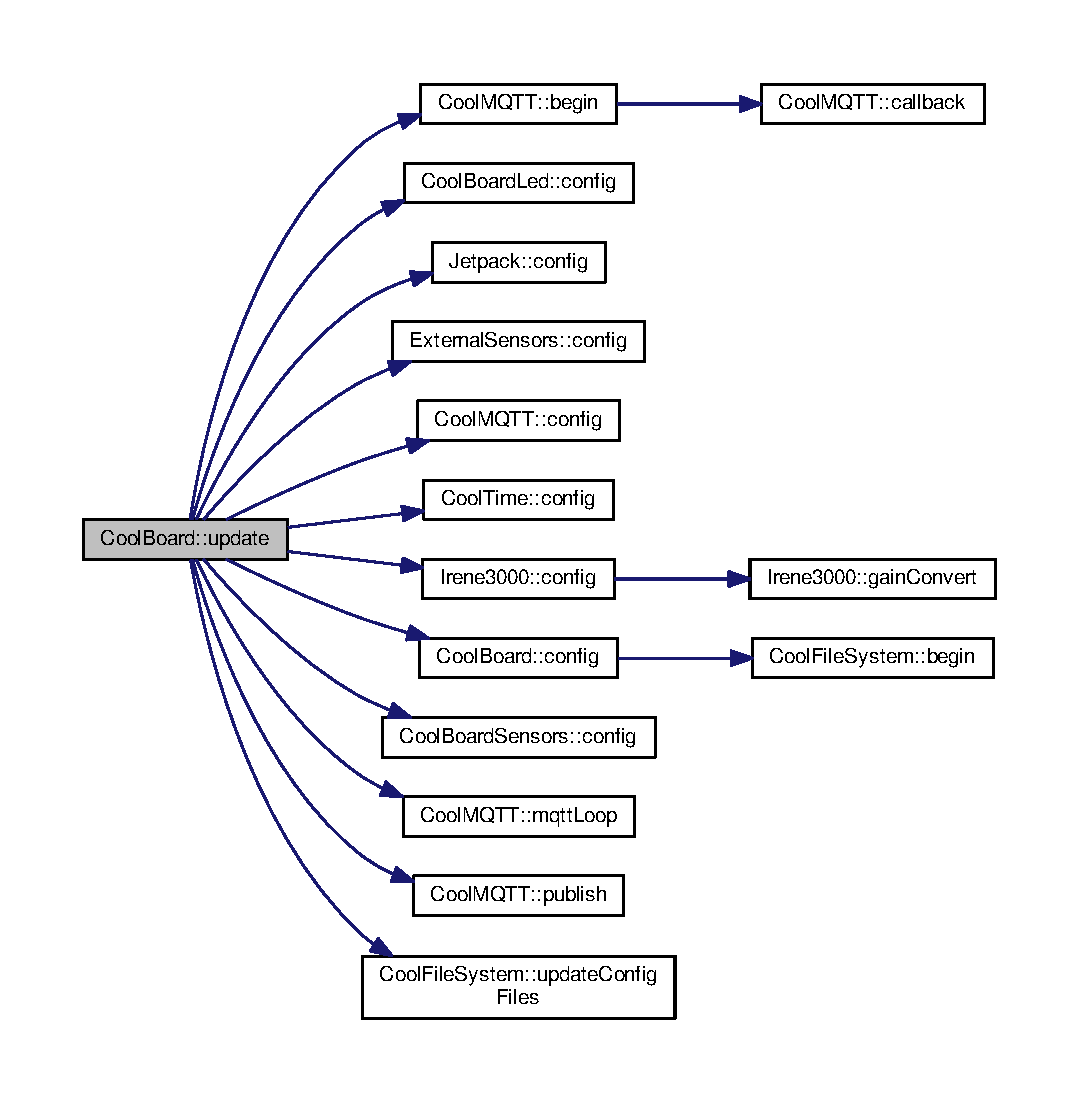
\includegraphics[width=350pt]{classCoolBoard_a8612756d3f73198cdde857a66f0fe690_cgraph}
\end{center}
\end{figure}
Here is the caller graph for this function\+:\nopagebreak
\begin{figure}[H]
\begin{center}
\leavevmode
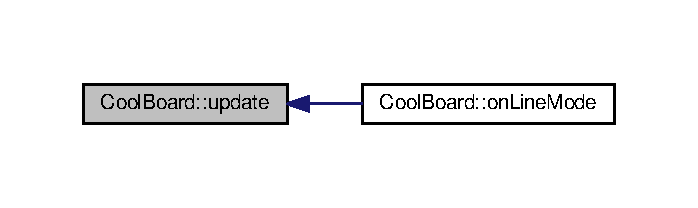
\includegraphics[width=335pt]{classCoolBoard_a8612756d3f73198cdde857a66f0fe690_icgraph}
\end{center}
\end{figure}
\mbox{\Hypertarget{classCoolBoard_ae7358fb6e623cfc81b775f5f1734909b}\label{classCoolBoard_ae7358fb6e623cfc81b775f5f1734909b}} 
\index{Cool\+Board@{Cool\+Board}!user\+Data@{user\+Data}}
\index{user\+Data@{user\+Data}!Cool\+Board@{Cool\+Board}}
\subsubsection{\texorpdfstring{user\+Data()}{userData()}}
{\footnotesize\ttfamily String Cool\+Board\+::user\+Data (\begin{DoxyParamCaption}{ }\end{DoxyParamCaption})}

\hyperlink{classCoolBoard_ae7358fb6e623cfc81b775f5f1734909b}{Cool\+Board\+::user\+Data()}\+: This method is provided to return the user\textquotesingle{}s data.

\begin{DoxyReturn}{Returns}
json string of the user\textquotesingle{}s data 
\end{DoxyReturn}


Definition at line 957 of file Cool\+Board.\+cpp.



References Cool\+Time\+::get\+E\+S\+Date(), Cool\+M\+Q\+T\+T\+::get\+User(), mqtt, and rtc.



Referenced by off\+Line\+Mode(), and on\+Line\+Mode().


\begin{DoxyCode}
958 \{
959 
960 \textcolor{preprocessor}{#if DEBUG == 1}
961 
962     Serial.println( F(\textcolor{stringliteral}{"Entering CoolBoard.userData() "}) );
963     Serial.println();
964 
965 \textcolor{preprocessor}{#endif}
966 
967     String tempMAC = WiFi.macAddress();
968 
969     tempMAC.replace(\textcolor{stringliteral}{":"}, \textcolor{stringliteral}{""});
970 
971     String userJson = \textcolor{stringliteral}{"\{\(\backslash\)"user\(\backslash\)":\(\backslash\)""};
972 
973     userJson += \hyperlink{classCoolBoard_a2399f44d7c23c1149a335cb3b46d90f1}{mqtt}.\hyperlink{classCoolMQTT_a373cc92fca7760d886f02d8a6e5b3f63}{getUser}();
974 
975     userJson += \textcolor{stringliteral}{"\(\backslash\)",\(\backslash\)"timestamp\(\backslash\)":\(\backslash\)""};
976 
977     userJson += \hyperlink{classCoolBoard_a50d2a6716879d64a85f3c6b44ad63275}{rtc}.\hyperlink{classCoolTime_ac4f32ee513c1328d984306645e8785a4}{getESDate}(); \textcolor{comment}{// "timestamp":"20yy-mm-ddThh:mm:ssZ"}
978 
979     userJson += \textcolor{stringliteral}{"\(\backslash\)",\(\backslash\)"mac\(\backslash\)":\(\backslash\)""};
980 
981     userJson += tempMAC;
982 
983     userJson += \textcolor{stringliteral}{"\(\backslash\)"\}"};
984 
985 \textcolor{preprocessor}{#if DEBUG == 1}
986 
987     Serial.println( F(\textcolor{stringliteral}{"userData is : "}) );
988     Serial.println(userJson);
989     Serial.println();
990 
991 \textcolor{preprocessor}{#endif  }
992     
993     \textcolor{keywordflow}{return}(userJson);
994     
995 \}
\end{DoxyCode}
Here is the call graph for this function\+:\nopagebreak
\begin{figure}[H]
\begin{center}
\leavevmode
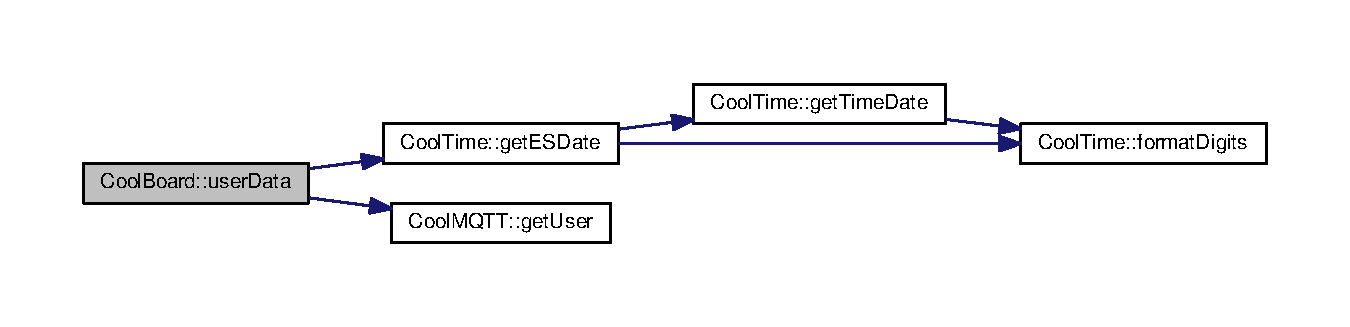
\includegraphics[width=350pt]{classCoolBoard_ae7358fb6e623cfc81b775f5f1734909b_cgraph}
\end{center}
\end{figure}
Here is the caller graph for this function\+:\nopagebreak
\begin{figure}[H]
\begin{center}
\leavevmode
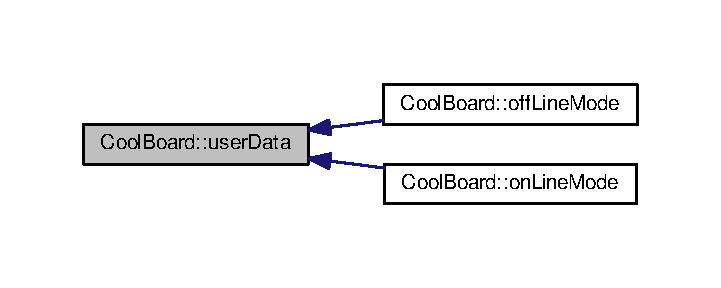
\includegraphics[width=346pt]{classCoolBoard_ae7358fb6e623cfc81b775f5f1734909b_icgraph}
\end{center}
\end{figure}


\subsection{Member Data Documentation}
\mbox{\Hypertarget{classCoolBoard_a7b835fafd449e5282f7f91d787a2dc15}\label{classCoolBoard_a7b835fafd449e5282f7f91d787a2dc15}} 
\index{Cool\+Board@{Cool\+Board}!answer@{answer}}
\index{answer@{answer}!Cool\+Board@{Cool\+Board}}
\subsubsection{\texorpdfstring{answer}{answer}}
{\footnotesize\ttfamily String Cool\+Board\+::answer =\char`\"{}\char`\"{}\hspace{0.3cm}{\ttfamily [private]}}



Definition at line 97 of file Cool\+Board.\+h.



Referenced by on\+Line\+Mode().

\mbox{\Hypertarget{classCoolBoard_a1b1d3c684a5baa56b08486e192fd8e97}\label{classCoolBoard_a1b1d3c684a5baa56b08486e192fd8e97}} 
\index{Cool\+Board@{Cool\+Board}!cool\+Board\+Led@{cool\+Board\+Led}}
\index{cool\+Board\+Led@{cool\+Board\+Led}!Cool\+Board@{Cool\+Board}}
\subsubsection{\texorpdfstring{cool\+Board\+Led}{coolBoardLed}}
{\footnotesize\ttfamily \hyperlink{classCoolBoardLed}{Cool\+Board\+Led} Cool\+Board\+::cool\+Board\+Led\hspace{0.3cm}{\ttfamily [private]}}



Definition at line 67 of file Cool\+Board.\+h.



Referenced by begin(), config(), connect(), off\+Line\+Mode(), on\+Line\+Mode(), read\+Sensors(), and update().

\mbox{\Hypertarget{classCoolBoard_af102be5288bd7f7a8e59b13f86e26a00}\label{classCoolBoard_af102be5288bd7f7a8e59b13f86e26a00}} 
\index{Cool\+Board@{Cool\+Board}!cool\+Board\+Sensors@{cool\+Board\+Sensors}}
\index{cool\+Board\+Sensors@{cool\+Board\+Sensors}!Cool\+Board@{Cool\+Board}}
\subsubsection{\texorpdfstring{cool\+Board\+Sensors}{coolBoardSensors}}
{\footnotesize\ttfamily \hyperlink{classCoolBoardSensors}{Cool\+Board\+Sensors} Cool\+Board\+::cool\+Board\+Sensors\hspace{0.3cm}{\ttfamily [private]}}



Definition at line 65 of file Cool\+Board.\+h.



Referenced by begin(), and read\+Sensors().

\mbox{\Hypertarget{classCoolBoard_a427fb753dd8575bdf821c70a5c63d695}\label{classCoolBoard_a427fb753dd8575bdf821c70a5c63d695}} 
\index{Cool\+Board@{Cool\+Board}!data@{data}}
\index{data@{data}!Cool\+Board@{Cool\+Board}}
\subsubsection{\texorpdfstring{data}{data}}
{\footnotesize\ttfamily String Cool\+Board\+::data =\char`\"{}\char`\"{}\hspace{0.3cm}{\ttfamily [private]}}



Definition at line 95 of file Cool\+Board.\+h.



Referenced by off\+Line\+Mode(), and on\+Line\+Mode().

\mbox{\Hypertarget{classCoolBoard_a09e26264839c65873eb56af476eff6b2}\label{classCoolBoard_a09e26264839c65873eb56af476eff6b2}} 
\index{Cool\+Board@{Cool\+Board}!external\+Sensors@{external\+Sensors}}
\index{external\+Sensors@{external\+Sensors}!Cool\+Board@{Cool\+Board}}
\subsubsection{\texorpdfstring{external\+Sensors}{externalSensors}}
{\footnotesize\ttfamily \hyperlink{classExternalSensors}{External\+Sensors} Cool\+Board\+::external\+Sensors\hspace{0.3cm}{\ttfamily [private]}}



Definition at line 79 of file Cool\+Board.\+h.



Referenced by begin(), and read\+Sensors().

\mbox{\Hypertarget{classCoolBoard_a638b00b76aeb819ecfd4c10b8cdd7bb7}\label{classCoolBoard_a638b00b76aeb819ecfd4c10b8cdd7bb7}} 
\index{Cool\+Board@{Cool\+Board}!external\+Sensors\+Active@{external\+Sensors\+Active}}
\index{external\+Sensors\+Active@{external\+Sensors\+Active}!Cool\+Board@{Cool\+Board}}
\subsubsection{\texorpdfstring{external\+Sensors\+Active}{externalSensorsActive}}
{\footnotesize\ttfamily bool Cool\+Board\+::external\+Sensors\+Active =0\hspace{0.3cm}{\ttfamily [private]}}



Definition at line 87 of file Cool\+Board.\+h.



Referenced by begin(), config(), print\+Conf(), and read\+Sensors().

\mbox{\Hypertarget{classCoolBoard_a42c2586fbb13ff7f06538e9284e8538d}\label{classCoolBoard_a42c2586fbb13ff7f06538e9284e8538d}} 
\index{Cool\+Board@{Cool\+Board}!file\+System@{file\+System}}
\index{file\+System@{file\+System}!Cool\+Board@{Cool\+Board}}
\subsubsection{\texorpdfstring{file\+System}{fileSystem}}
{\footnotesize\ttfamily \hyperlink{classCoolFileSystem}{Cool\+File\+System} Cool\+Board\+::file\+System\hspace{0.3cm}{\ttfamily [private]}}



Definition at line 63 of file Cool\+Board.\+h.



Referenced by config(), off\+Line\+Mode(), on\+Line\+Mode(), and update().

\mbox{\Hypertarget{classCoolBoard_ad103718ce316006c4695b8eb312eaf11}\label{classCoolBoard_ad103718ce316006c4695b8eb312eaf11}} 
\index{Cool\+Board@{Cool\+Board}!irene3000@{irene3000}}
\index{irene3000@{irene3000}!Cool\+Board@{Cool\+Board}}
\subsubsection{\texorpdfstring{irene3000}{irene3000}}
{\footnotesize\ttfamily \hyperlink{classIrene3000}{Irene3000} Cool\+Board\+::irene3000\hspace{0.3cm}{\ttfamily [private]}}



Definition at line 77 of file Cool\+Board.\+h.



Referenced by begin(), and read\+Sensors().

\mbox{\Hypertarget{classCoolBoard_a9c3f7ac625481ee2ae802a25d97a4ae0}\label{classCoolBoard_a9c3f7ac625481ee2ae802a25d97a4ae0}} 
\index{Cool\+Board@{Cool\+Board}!irene\+Active@{irene\+Active}}
\index{irene\+Active@{irene\+Active}!Cool\+Board@{Cool\+Board}}
\subsubsection{\texorpdfstring{irene\+Active}{ireneActive}}
{\footnotesize\ttfamily bool Cool\+Board\+::irene\+Active =0\hspace{0.3cm}{\ttfamily [private]}}



Definition at line 83 of file Cool\+Board.\+h.



Referenced by begin(), config(), print\+Conf(), and read\+Sensors().

\mbox{\Hypertarget{classCoolBoard_a30b1357881b01ccbec676856a91e48e9}\label{classCoolBoard_a30b1357881b01ccbec676856a91e48e9}} 
\index{Cool\+Board@{Cool\+Board}!jet\+Pack@{jet\+Pack}}
\index{jet\+Pack@{jet\+Pack}!Cool\+Board@{Cool\+Board}}
\subsubsection{\texorpdfstring{jet\+Pack}{jetPack}}
{\footnotesize\ttfamily \hyperlink{classJetpack}{Jetpack} Cool\+Board\+::jet\+Pack\hspace{0.3cm}{\ttfamily [private]}}



Definition at line 75 of file Cool\+Board.\+h.



Referenced by begin(), off\+Line\+Mode(), and on\+Line\+Mode().

\mbox{\Hypertarget{classCoolBoard_a9be03a913d26e558328935ca3b59a75e}\label{classCoolBoard_a9be03a913d26e558328935ca3b59a75e}} 
\index{Cool\+Board@{Cool\+Board}!jetpack\+Active@{jetpack\+Active}}
\index{jetpack\+Active@{jetpack\+Active}!Cool\+Board@{Cool\+Board}}
\subsubsection{\texorpdfstring{jetpack\+Active}{jetpackActive}}
{\footnotesize\ttfamily bool Cool\+Board\+::jetpack\+Active =0\hspace{0.3cm}{\ttfamily [private]}}



Definition at line 85 of file Cool\+Board.\+h.



Referenced by begin(), config(), off\+Line\+Mode(), on\+Line\+Mode(), and print\+Conf().

\mbox{\Hypertarget{classCoolBoard_a84bc94413b64973e4aba8c467c97006c}\label{classCoolBoard_a84bc94413b64973e4aba8c467c97006c}} 
\index{Cool\+Board@{Cool\+Board}!log\+Interval@{log\+Interval}}
\index{log\+Interval@{log\+Interval}!Cool\+Board@{Cool\+Board}}
\subsubsection{\texorpdfstring{log\+Interval}{logInterval}}
{\footnotesize\ttfamily unsigned long Cool\+Board\+::log\+Interval =1\hspace{0.3cm}{\ttfamily [private]}}



Definition at line 91 of file Cool\+Board.\+h.



Referenced by config(), get\+Log\+Interval(), and print\+Conf().

\mbox{\Hypertarget{classCoolBoard_a2399f44d7c23c1149a335cb3b46d90f1}\label{classCoolBoard_a2399f44d7c23c1149a335cb3b46d90f1}} 
\index{Cool\+Board@{Cool\+Board}!mqtt@{mqtt}}
\index{mqtt@{mqtt}!Cool\+Board@{Cool\+Board}}
\subsubsection{\texorpdfstring{mqtt}{mqtt}}
{\footnotesize\ttfamily \hyperlink{classCoolMQTT}{Cool\+M\+Q\+TT} Cool\+Board\+::mqtt\hspace{0.3cm}{\ttfamily [private]}}



Definition at line 73 of file Cool\+Board.\+h.



Referenced by begin(), connect(), on\+Line\+Mode(), update(), and user\+Data().

\mbox{\Hypertarget{classCoolBoard_a50d2a6716879d64a85f3c6b44ad63275}\label{classCoolBoard_a50d2a6716879d64a85f3c6b44ad63275}} 
\index{Cool\+Board@{Cool\+Board}!rtc@{rtc}}
\index{rtc@{rtc}!Cool\+Board@{Cool\+Board}}
\subsubsection{\texorpdfstring{rtc}{rtc}}
{\footnotesize\ttfamily \hyperlink{classCoolTime}{Cool\+Time} Cool\+Board\+::rtc\hspace{0.3cm}{\ttfamily [private]}}



Definition at line 69 of file Cool\+Board.\+h.



Referenced by begin(), on\+Line\+Mode(), read\+Sensors(), and user\+Data().

\mbox{\Hypertarget{classCoolBoard_a7a8d8d3d316220cdd049cd63c1aa8fe6}\label{classCoolBoard_a7a8d8d3d316220cdd049cd63c1aa8fe6}} 
\index{Cool\+Board@{Cool\+Board}!server\+Time\+Out@{server\+Time\+Out}}
\index{server\+Time\+Out@{server\+Time\+Out}!Cool\+Board@{Cool\+Board}}
\subsubsection{\texorpdfstring{server\+Time\+Out}{serverTimeOut}}
{\footnotesize\ttfamily int Cool\+Board\+::server\+Time\+Out =180\hspace{0.3cm}{\ttfamily [private]}}



Definition at line 93 of file Cool\+Board.\+h.



Referenced by config(), and print\+Conf().

\mbox{\Hypertarget{classCoolBoard_a0a51b2287139f66c738101fb53139230}\label{classCoolBoard_a0a51b2287139f66c738101fb53139230}} 
\index{Cool\+Board@{Cool\+Board}!sleep\+Active@{sleep\+Active}}
\index{sleep\+Active@{sleep\+Active}!Cool\+Board@{Cool\+Board}}
\subsubsection{\texorpdfstring{sleep\+Active}{sleepActive}}
{\footnotesize\ttfamily bool Cool\+Board\+::sleep\+Active =0\hspace{0.3cm}{\ttfamily [private]}}



Definition at line 89 of file Cool\+Board.\+h.



Referenced by config(), on\+Line\+Mode(), and print\+Conf().

\mbox{\Hypertarget{classCoolBoard_a6395459131d6889a3005f79c7a35e964}\label{classCoolBoard_a6395459131d6889a3005f79c7a35e964}} 
\index{Cool\+Board@{Cool\+Board}!user\+Active@{user\+Active}}
\index{user\+Active@{user\+Active}!Cool\+Board@{Cool\+Board}}
\subsubsection{\texorpdfstring{user\+Active}{userActive}}
{\footnotesize\ttfamily bool Cool\+Board\+::user\+Active =0\hspace{0.3cm}{\ttfamily [private]}}



Definition at line 81 of file Cool\+Board.\+h.



Referenced by config(), off\+Line\+Mode(), on\+Line\+Mode(), and print\+Conf().

\mbox{\Hypertarget{classCoolBoard_acd88e6003606b47479ebba81e4aceeca}\label{classCoolBoard_acd88e6003606b47479ebba81e4aceeca}} 
\index{Cool\+Board@{Cool\+Board}!wifi\+Manager@{wifi\+Manager}}
\index{wifi\+Manager@{wifi\+Manager}!Cool\+Board@{Cool\+Board}}
\subsubsection{\texorpdfstring{wifi\+Manager}{wifiManager}}
{\footnotesize\ttfamily \hyperlink{classCoolWifi}{Cool\+Wifi} Cool\+Board\+::wifi\+Manager\hspace{0.3cm}{\ttfamily [private]}}



Definition at line 71 of file Cool\+Board.\+h.



Referenced by begin(), and connect().



The documentation for this class was generated from the following files\+:\begin{DoxyCompactItemize}
\item 
/home/ashiroji/\+Arduino/libraries/\+Cool\+Board/\hyperlink{CoolBoard_8h}{Cool\+Board.\+h}\item 
/home/ashiroji/\+Arduino/libraries/\+Cool\+Board/\hyperlink{CoolBoard_8cpp}{Cool\+Board.\+cpp}\end{DoxyCompactItemize}

\hypertarget{classCoolBoardLed}{}\section{Cool\+Board\+Led Class Reference}
\label{classCoolBoardLed}\index{Cool\+Board\+Led@{Cool\+Board\+Led}}


This class handles the led in the Sensor Board.  




{\ttfamily \#include $<$Cool\+Board\+Led.\+h$>$}



Collaboration diagram for Cool\+Board\+Led\+:
\nopagebreak
\begin{figure}[H]
\begin{center}
\leavevmode
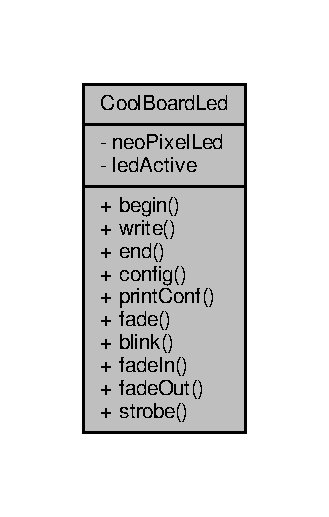
\includegraphics[width=158pt]{classCoolBoardLed__coll__graph}
\end{center}
\end{figure}
\subsection*{Public Member Functions}
\begin{DoxyCompactItemize}
\item 
void \hyperlink{classCoolBoardLed_ae3cbde8affcc6f011cbd698c8ef911f6}{begin} ()
\item 
void \hyperlink{classCoolBoardLed_a30fadd4cbec17ceea428bf7a32207e87}{write} (int R, int G, int B)
\item 
void \hyperlink{classCoolBoardLed_a69f323359e0c9f797422f2152b5d41ef}{end} ()
\item 
bool \hyperlink{classCoolBoardLed_a1b60e5e30bea96c49ed62ed1bf1ffc8b}{config} ()
\item 
void \hyperlink{classCoolBoardLed_a8ed3053a36f0ed4a131f43b5b17efb61}{print\+Conf} ()
\item 
void \hyperlink{classCoolBoardLed_a6dbfe23988f43e1242cd05e69b13ff30}{color\+Fade} (int R, int G, int B, int T)
\item 
void \hyperlink{classCoolBoardLed_a27706bc029f6a126c55d0b91624ad7fa}{blink} (int R, int G, int B, int T)
\item 
void \hyperlink{classCoolBoardLed_aec915442a8441c7cd45c3279d3ff8821}{fade\+In} (int R, int G, int B, int T)
\item 
void \hyperlink{classCoolBoardLed_a27c4e14fa2cd3639c0844152cea98887}{fade\+Out} (int R, int G, int B, int T)
\item 
void \hyperlink{classCoolBoardLed_adc08c0ac07473499971c503d300f0413}{strobe} (int R, int G, int B, int T)
\end{DoxyCompactItemize}
\subsection*{Private Attributes}
\begin{DoxyCompactItemize}
\item 
Neo\+Pixel\+Bus$<$ Neo\+Grb\+Feature, Neo800\+Kbps\+Method $>$ $\ast$ \hyperlink{classCoolBoardLed_ac2c13fa462a010cd9242bf297c013923}{neo\+Pixel\+Led} = N\+U\+LL
\item 
byte \hyperlink{classCoolBoardLed_a5f17c135516fcf4b44ea8a096ba0177a}{led\+Active} =0
\end{DoxyCompactItemize}


\subsection{Detailed Description}
This class handles the led in the Sensor Board. 

Definition at line 20 of file Cool\+Board\+Led.\+h.



\subsection{Member Function Documentation}
\mbox{\Hypertarget{classCoolBoardLed_ae3cbde8affcc6f011cbd698c8ef911f6}\label{classCoolBoardLed_ae3cbde8affcc6f011cbd698c8ef911f6}} 
\index{Cool\+Board\+Led@{Cool\+Board\+Led}!begin@{begin}}
\index{begin@{begin}!Cool\+Board\+Led@{Cool\+Board\+Led}}
\subsubsection{\texorpdfstring{begin()}{begin()}}
{\footnotesize\ttfamily void Cool\+Board\+Led\+::begin (\begin{DoxyParamCaption}{ }\end{DoxyParamCaption})}

\hyperlink{classCoolBoardLed_ae3cbde8affcc6f011cbd698c8ef911f6}{Cool\+Board\+Led\+::begin()}\+: This method is provided to start the Led Object by setting the correct pin and creating a dynamic neo\+Pixel\+Bus 

Definition at line 218 of file Cool\+Board\+Led.\+cpp.



References neo\+Pixel\+Led.



Referenced by Cool\+Board\+::begin().


\begin{DoxyCode}
219 \{
220 
221 \textcolor{preprocessor}{#if DEBUG == 1}
222 
223     Serial.println( F(\textcolor{stringliteral}{"Entering CoolBoardLed.begin() "}) );
224 
225 \textcolor{preprocessor}{#endif}
226 
227     pinMode(5,OUTPUT);
228     digitalWrite(5,HIGH);
229     \hyperlink{classCoolBoardLed_ac2c13fa462a010cd9242bf297c013923}{neoPixelLed} = \textcolor{keyword}{new} NeoPixelBus<NeoGrbFeature, Neo800KbpsMethod>(1,2); 
230     \hyperlink{classCoolBoardLed_ac2c13fa462a010cd9242bf297c013923}{neoPixelLed}->Begin();
231     \hyperlink{classCoolBoardLed_ac2c13fa462a010cd9242bf297c013923}{neoPixelLed}->Show();
232 \} 
\end{DoxyCode}
Here is the caller graph for this function\+:
\nopagebreak
\begin{figure}[H]
\begin{center}
\leavevmode
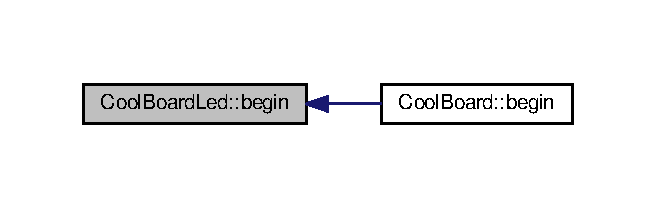
\includegraphics[width=315pt]{classCoolBoardLed_ae3cbde8affcc6f011cbd698c8ef911f6_icgraph}
\end{center}
\end{figure}
\mbox{\Hypertarget{classCoolBoardLed_a27706bc029f6a126c55d0b91624ad7fa}\label{classCoolBoardLed_a27706bc029f6a126c55d0b91624ad7fa}} 
\index{Cool\+Board\+Led@{Cool\+Board\+Led}!blink@{blink}}
\index{blink@{blink}!Cool\+Board\+Led@{Cool\+Board\+Led}}
\subsubsection{\texorpdfstring{blink()}{blink()}}
{\footnotesize\ttfamily void Cool\+Board\+Led\+::blink (\begin{DoxyParamCaption}\item[{int}]{R,  }\item[{int}]{G,  }\item[{int}]{B,  }\item[{int}]{T }\end{DoxyParamCaption})}

Cool\+Board\+Led\+::blink( Red , Green , Blue , Time in seconds )\+: Blink animation\+: Led On for T seconds Led off 

Definition at line 71 of file Cool\+Board\+Led.\+cpp.



References neo\+Pixel\+Led.


\begin{DoxyCode}
72 \{
73 
74 \textcolor{preprocessor}{#if DEBUG == 1}
75 
76     Serial.println( F(\textcolor{stringliteral}{"Entering CoolBoardLed.blink()"}));
77     Serial.println();
78     Serial.print( F(\textcolor{stringliteral}{"R : "}));
79     Serial.println(R);
80     Serial.print( F(\textcolor{stringliteral}{"G : "}) );
81     Serial.println(G);
82     Serial.print( F(\textcolor{stringliteral}{"B : "}) );
83     Serial.println(B);
84     Serial.print( F(\textcolor{stringliteral}{"Time :"}) );
85     Serial.println(T);
86     Serial.println();
87 
88 \textcolor{preprocessor}{#endif  }
89 
90     \hyperlink{classCoolBoardLed_ac2c13fa462a010cd9242bf297c013923}{neoPixelLed}->SetPixelColor(0, RgbColor(R, G, B));
91     \hyperlink{classCoolBoardLed_ac2c13fa462a010cd9242bf297c013923}{neoPixelLed}->Show();
92     delay(T);
93     \hyperlink{classCoolBoardLed_ac2c13fa462a010cd9242bf297c013923}{neoPixelLed}->SetPixelColor(0, RgbColor(0, 0, 0));
94     \hyperlink{classCoolBoardLed_ac2c13fa462a010cd9242bf297c013923}{neoPixelLed}->Show();
95 \}
\end{DoxyCode}
\mbox{\Hypertarget{classCoolBoardLed_a6dbfe23988f43e1242cd05e69b13ff30}\label{classCoolBoardLed_a6dbfe23988f43e1242cd05e69b13ff30}} 
\index{Cool\+Board\+Led@{Cool\+Board\+Led}!color\+Fade@{color\+Fade}}
\index{color\+Fade@{color\+Fade}!Cool\+Board\+Led@{Cool\+Board\+Led}}
\subsubsection{\texorpdfstring{color\+Fade()}{colorFade()}}
{\footnotesize\ttfamily void Cool\+Board\+Led\+::color\+Fade (\begin{DoxyParamCaption}\item[{int}]{R,  }\item[{int}]{G,  }\item[{int}]{B,  }\item[{int}]{T }\end{DoxyParamCaption})}

\hyperlink{classCoolBoardLed_a6dbfe23988f43e1242cd05e69b13ff30}{Cool\+Board\+Led\+::color\+Fade} ( Red , Green , Blue, Time in seconds )\+: color\+Fade animation\+: Fade In over T(seconds) Fade Out over T(seconds) 

Definition at line 33 of file Cool\+Board\+Led.\+cpp.



References neo\+Pixel\+Led.


\begin{DoxyCode}
34 \{
35 
36 \textcolor{preprocessor}{#if DEBUG == 1}
37 
38     Serial.println( F(\textcolor{stringliteral}{"Entering CoolBoardLed.colorFade()"}) );
39     Serial.println();
40     Serial.print( F(\textcolor{stringliteral}{"R : "}) );
41     Serial.println(R);
42     Serial.print( F(\textcolor{stringliteral}{"G : "}) );
43     Serial.println(G);
44     Serial.print( F(\textcolor{stringliteral}{"B : "}) );
45     Serial.println(B);
46     Serial.print( F(\textcolor{stringliteral}{"Time : "}) );
47     Serial.println(T);
48     Serial.println();
49 
50 \textcolor{preprocessor}{#endif  }
51 
52     \textcolor{keywordflow}{for} (\textcolor{keywordtype}{int} k = 0; k < 1000; k++) 
53     \{
54         \hyperlink{classCoolBoardLed_ac2c13fa462a010cd9242bf297c013923}{neoPixelLed}->SetPixelColor(0, RgbColor(k * R / 1000, k * G / 1000, k * B / 1000));
55         \hyperlink{classCoolBoardLed_ac2c13fa462a010cd9242bf297c013923}{neoPixelLed}->Show();
56         delay(T);
57     \}
58     \textcolor{keywordflow}{for} (\textcolor{keywordtype}{int} k = 1000; k >= 0; k--) 
59     \{
60         \hyperlink{classCoolBoardLed_ac2c13fa462a010cd9242bf297c013923}{neoPixelLed}->SetPixelColor(0, RgbColor(k * R / 1000, k * G / 1000, k * B / 1000));
61         \hyperlink{classCoolBoardLed_ac2c13fa462a010cd9242bf297c013923}{neoPixelLed}->Show();
62         delay(T);
63     \}
64 \}
\end{DoxyCode}
\mbox{\Hypertarget{classCoolBoardLed_a1b60e5e30bea96c49ed62ed1bf1ffc8b}\label{classCoolBoardLed_a1b60e5e30bea96c49ed62ed1bf1ffc8b}} 
\index{Cool\+Board\+Led@{Cool\+Board\+Led}!config@{config}}
\index{config@{config}!Cool\+Board\+Led@{Cool\+Board\+Led}}
\subsubsection{\texorpdfstring{config()}{config()}}
{\footnotesize\ttfamily bool Cool\+Board\+Led\+::config (\begin{DoxyParamCaption}{ }\end{DoxyParamCaption})}

\hyperlink{classCoolBoardLed_a1b60e5e30bea96c49ed62ed1bf1ffc8b}{Cool\+Board\+Led\+::config()}\+: This method is provided to configure the Led Object \+: -\/led\+Active=0 \+: deactivated -\/led\+Active=1 \+: activated \begin{DoxyReturn}{Returns}
true if the configuration done, false otherwise 
\end{DoxyReturn}


Definition at line 268 of file Cool\+Board\+Led.\+cpp.



References led\+Active.



Referenced by Cool\+Board\+::begin(), and Cool\+Board\+::update().


\begin{DoxyCode}
269 \{
270 
271 \textcolor{preprocessor}{#if DEBUG == 1 }
272         
273     Serial.println( F(\textcolor{stringliteral}{"Entering CoolBoardLed.config()"}) );
274     Serial.println();
275 
276 \textcolor{preprocessor}{#endif}
277     
278     File coolBoardLedConfig = SPIFFS.open(\textcolor{stringliteral}{"/coolBoardLedConfig.json"}, \textcolor{stringliteral}{"r"});
279 
280     \textcolor{keywordflow}{if} (!coolBoardLedConfig) 
281     \{
282     
283 \textcolor{preprocessor}{    #if DEBUG == 1}
284 
285         Serial.println( F(\textcolor{stringliteral}{"failed to read /coolBoardLedConfig.json"}) );
286         Serial.println();
287 
288 \textcolor{preprocessor}{    #endif}
289 
290         \textcolor{keywordflow}{return}(\textcolor{keyword}{false});
291     \}
292     \textcolor{keywordflow}{else}
293     \{
294         \textcolor{keywordtype}{size\_t} size = coolBoardLedConfig.size();
295         \textcolor{comment}{// Allocate a buffer to store contents of the file.}
296         std::unique\_ptr<char[]> buf(\textcolor{keyword}{new} \textcolor{keywordtype}{char}[size]);
297 
298         coolBoardLedConfig.readBytes(buf.get(), size);
299         DynamicJsonBuffer jsonBuffer;
300         JsonObject& json = jsonBuffer.parseObject(buf.get());
301         \textcolor{keywordflow}{if} (!json.success()) 
302         \{
303         
304 \textcolor{preprocessor}{        #if DEBUG == 1}
305 
306             Serial.println( F(\textcolor{stringliteral}{"failed to parse json"}) );
307             Serial.println();
308         
309 \textcolor{preprocessor}{        #endif}
310 
311             \textcolor{keywordflow}{return}(\textcolor{keyword}{false});
312         \} 
313         \textcolor{keywordflow}{else}
314         \{
315         
316 \textcolor{preprocessor}{        #if DEBUG == 1}
317     
318             Serial.println( F(\textcolor{stringliteral}{"read configuration file : "}) );
319             json.printTo(Serial);
320             Serial.println();
321         
322 \textcolor{preprocessor}{        #endif}
323   
324             \textcolor{keywordflow}{if}(json[\textcolor{stringliteral}{"ledActive"}].success() )
325             \{
326                 this->\hyperlink{classCoolBoardLed_a5f17c135516fcf4b44ea8a096ba0177a}{ledActive} = json[\textcolor{stringliteral}{"ledActive"}]; 
327             \}
328             \textcolor{keywordflow}{else}
329             \{
330                 this->\hyperlink{classCoolBoardLed_a5f17c135516fcf4b44ea8a096ba0177a}{ledActive}=this->\hyperlink{classCoolBoardLed_a5f17c135516fcf4b44ea8a096ba0177a}{ledActive};          
331             \}
332             
333             json[\textcolor{stringliteral}{"ledActive"}]=this->\hyperlink{classCoolBoardLed_a5f17c135516fcf4b44ea8a096ba0177a}{ledActive};
334             coolBoardLedConfig.close();
335             
336             coolBoardLedConfig = SPIFFS.open(\textcolor{stringliteral}{"/coolBoardLedConfig.json"}, \textcolor{stringliteral}{"w"});
337             \textcolor{keywordflow}{if}(!coolBoardLedConfig)
338             \{
339             
340 \textcolor{preprocessor}{            #if DEBUG == 1 }
341 
342                 Serial.println( F(\textcolor{stringliteral}{"failed to write to /coolBoardLedConfig.json"}) );
343                 Serial.println();
344 
345 \textcolor{preprocessor}{            #endif}
346 
347                 \textcolor{keywordflow}{return}(\textcolor{keyword}{false});          
348             \}
349 
350             json.printTo(coolBoardLedConfig);
351             coolBoardLedConfig.close();
352 
353 \textcolor{preprocessor}{        #if DEBUG == 1}
354     
355             Serial.println( F(\textcolor{stringliteral}{"saved Led Config is : "}) );
356             json.printTo(Serial);
357             Serial.println();
358 
359 \textcolor{preprocessor}{        #endif}
360 
361             \textcolor{keywordflow}{return}(\textcolor{keyword}{true}); 
362         \}
363     \}   
364 
365 \}               
\end{DoxyCode}
Here is the caller graph for this function\+:
\nopagebreak
\begin{figure}[H]
\begin{center}
\leavevmode
\includegraphics[width=350pt]{classCoolBoardLed_a1b60e5e30bea96c49ed62ed1bf1ffc8b_icgraph}
\end{center}
\end{figure}
\mbox{\Hypertarget{classCoolBoardLed_a69f323359e0c9f797422f2152b5d41ef}\label{classCoolBoardLed_a69f323359e0c9f797422f2152b5d41ef}} 
\index{Cool\+Board\+Led@{Cool\+Board\+Led}!end@{end}}
\index{end@{end}!Cool\+Board\+Led@{Cool\+Board\+Led}}
\subsubsection{\texorpdfstring{end()}{end()}}
{\footnotesize\ttfamily void Cool\+Board\+Led\+::end (\begin{DoxyParamCaption}{ }\end{DoxyParamCaption})}

\hyperlink{classCoolBoardLed_a69f323359e0c9f797422f2152b5d41ef}{Cool\+Board\+Led\+::end()} \+: this method is provided to delete the dynamically created neo\+Pixel\+Led 

Definition at line 199 of file Cool\+Board\+Led.\+cpp.



References neo\+Pixel\+Led.


\begin{DoxyCode}
200 \{
201 
202 \textcolor{preprocessor}{#if DEBUG == 1 }
203     
204     Serial.println( F(\textcolor{stringliteral}{"Entering CoolBoardLed.end()"}) );
205 
206 \textcolor{preprocessor}{#endif}
207 
208     \textcolor{keyword}{delete} \hyperlink{classCoolBoardLed_ac2c13fa462a010cd9242bf297c013923}{neoPixelLed};
209 \}
\end{DoxyCode}
\mbox{\Hypertarget{classCoolBoardLed_aec915442a8441c7cd45c3279d3ff8821}\label{classCoolBoardLed_aec915442a8441c7cd45c3279d3ff8821}} 
\index{Cool\+Board\+Led@{Cool\+Board\+Led}!fade\+In@{fade\+In}}
\index{fade\+In@{fade\+In}!Cool\+Board\+Led@{Cool\+Board\+Led}}
\subsubsection{\texorpdfstring{fade\+In()}{fadeIn()}}
{\footnotesize\ttfamily void Cool\+Board\+Led\+::fade\+In (\begin{DoxyParamCaption}\item[{int}]{R,  }\item[{int}]{G,  }\item[{int}]{B,  }\item[{int}]{T }\end{DoxyParamCaption})}

Cool\+Board\+Led\+::fade\+In(\+Red , Green , Blue , Time in seconds) Fade In animation\+: gradual increase over T(seconds) 

Definition at line 101 of file Cool\+Board\+Led.\+cpp.



References neo\+Pixel\+Led.


\begin{DoxyCode}
102 \{
103 
104 \textcolor{preprocessor}{#if DEBUG == 1}
105 
106     Serial.println( F(\textcolor{stringliteral}{"Entering CoolBoardLed.fadeIn()"}) );
107     Serial.println();
108     Serial.print( F(\textcolor{stringliteral}{"R : "}) );
109     Serial.println(R);
110     Serial.print( F(\textcolor{stringliteral}{"G : "}) );
111     Serial.println(G);
112     Serial.print( F(\textcolor{stringliteral}{"B : "}) );
113     Serial.println(B);
114     Serial.print( F(\textcolor{stringliteral}{"Time :"}) );
115     Serial.println(T);
116     Serial.println();
117 
118 \textcolor{preprocessor}{#endif  }
119 
120     \textcolor{keywordflow}{for} (\textcolor{keywordtype}{int} k = 0; k < 1000; k++) 
121     \{
122         \hyperlink{classCoolBoardLed_ac2c13fa462a010cd9242bf297c013923}{neoPixelLed}->SetPixelColor(0, RgbColor(k * R / 1000, k * G / 1000, k * B / 1000));
123         \hyperlink{classCoolBoardLed_ac2c13fa462a010cd9242bf297c013923}{neoPixelLed}->Show();
124         delay(T);
125     \}
126 \}
\end{DoxyCode}
\mbox{\Hypertarget{classCoolBoardLed_a27c4e14fa2cd3639c0844152cea98887}\label{classCoolBoardLed_a27c4e14fa2cd3639c0844152cea98887}} 
\index{Cool\+Board\+Led@{Cool\+Board\+Led}!fade\+Out@{fade\+Out}}
\index{fade\+Out@{fade\+Out}!Cool\+Board\+Led@{Cool\+Board\+Led}}
\subsubsection{\texorpdfstring{fade\+Out()}{fadeOut()}}
{\footnotesize\ttfamily void Cool\+Board\+Led\+::fade\+Out (\begin{DoxyParamCaption}\item[{int}]{R,  }\item[{int}]{G,  }\item[{int}]{B,  }\item[{int}]{T }\end{DoxyParamCaption})}

Cool\+Board\+Led\+::fade\+Out( Red , Green , Blue , Time in seconds) Fade Out animation\+: gradual decrease over T(seconds) 

Definition at line 132 of file Cool\+Board\+Led.\+cpp.



References neo\+Pixel\+Led.


\begin{DoxyCode}
133 \{
134 
135 \textcolor{preprocessor}{#if DEBUG == 1 }
136 
137     Serial.println( F(\textcolor{stringliteral}{"Entering CoolBoardLed.fadeOut()"} ) );
138     Serial.println();
139     Serial.print( F(\textcolor{stringliteral}{"R : "}) );
140     Serial.println(R);
141     Serial.print( F(\textcolor{stringliteral}{"G : "}) );
142     Serial.println(G);
143     Serial.print( F(\textcolor{stringliteral}{"B : "}) );
144     Serial.println(B);
145     Serial.print( F(\textcolor{stringliteral}{"Time :"}) );
146     Serial.println(T);
147     Serial.println();
148 
149 \textcolor{preprocessor}{#endif  }
150 
151 
152     \textcolor{keywordflow}{for} (\textcolor{keywordtype}{int} k = 1000; k >= 0; k--) 
153     \{
154         \hyperlink{classCoolBoardLed_ac2c13fa462a010cd9242bf297c013923}{neoPixelLed}->SetPixelColor(0, RgbColor(k * R / 1000, k * G / 1000, k * B / 1000));
155         \hyperlink{classCoolBoardLed_ac2c13fa462a010cd9242bf297c013923}{neoPixelLed}->Show();
156         delay(T);
157     \}
158 \}
\end{DoxyCode}
\mbox{\Hypertarget{classCoolBoardLed_a8ed3053a36f0ed4a131f43b5b17efb61}\label{classCoolBoardLed_a8ed3053a36f0ed4a131f43b5b17efb61}} 
\index{Cool\+Board\+Led@{Cool\+Board\+Led}!print\+Conf@{print\+Conf}}
\index{print\+Conf@{print\+Conf}!Cool\+Board\+Led@{Cool\+Board\+Led}}
\subsubsection{\texorpdfstring{print\+Conf()}{printConf()}}
{\footnotesize\ttfamily void Cool\+Board\+Led\+::print\+Conf (\begin{DoxyParamCaption}{ }\end{DoxyParamCaption})}

\hyperlink{classCoolBoardLed_a8ed3053a36f0ed4a131f43b5b17efb61}{Cool\+Board\+Led\+::print\+Conf()}\+: This method is provided to print the Led Object Configuration to the Serial Monitor 

Definition at line 373 of file Cool\+Board\+Led.\+cpp.



References led\+Active.



Referenced by Cool\+Board\+::begin().


\begin{DoxyCode}
374 \{
375 
376 \textcolor{preprocessor}{#if DEBUG == 1 }
377 
378     Serial.println( F(\textcolor{stringliteral}{"Entering CoolBoardLed.printConf()"}) );
379     Serial.println();
380 
381 \textcolor{preprocessor}{#endif}
382 
383     Serial.println(\textcolor{stringliteral}{"Led Configuration"});
384 
385     Serial.print(\textcolor{stringliteral}{"ledActive : "});
386     Serial.println(\hyperlink{classCoolBoardLed_a5f17c135516fcf4b44ea8a096ba0177a}{ledActive});
387 
388     Serial.println();   
389 \}
\end{DoxyCode}
Here is the caller graph for this function\+:
\nopagebreak
\begin{figure}[H]
\begin{center}
\leavevmode
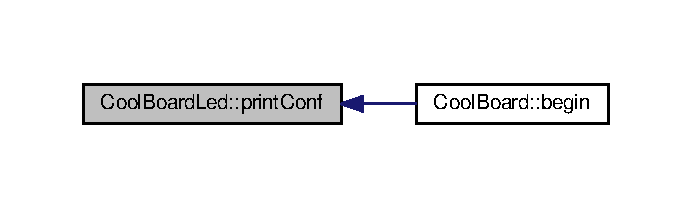
\includegraphics[width=332pt]{classCoolBoardLed_a8ed3053a36f0ed4a131f43b5b17efb61_icgraph}
\end{center}
\end{figure}
\mbox{\Hypertarget{classCoolBoardLed_adc08c0ac07473499971c503d300f0413}\label{classCoolBoardLed_adc08c0ac07473499971c503d300f0413}} 
\index{Cool\+Board\+Led@{Cool\+Board\+Led}!strobe@{strobe}}
\index{strobe@{strobe}!Cool\+Board\+Led@{Cool\+Board\+Led}}
\subsubsection{\texorpdfstring{strobe()}{strobe()}}
{\footnotesize\ttfamily void Cool\+Board\+Led\+::strobe (\begin{DoxyParamCaption}\item[{int}]{R,  }\item[{int}]{G,  }\item[{int}]{B,  }\item[{int}]{T }\end{DoxyParamCaption})}

Cool\+Board\+Led\+::strobe(\+Red , Green , Blue , Time in seconds) Strobe animation\+: blinks over T(seconds) 

Definition at line 164 of file Cool\+Board\+Led.\+cpp.



References neo\+Pixel\+Led.


\begin{DoxyCode}
165 \{
166 
167 \textcolor{preprocessor}{#if DEBUG == 1}
168 
169     Serial.println( F(\textcolor{stringliteral}{"Entering CoolBoardLed.strobe()"}) );
170     Serial.println();
171     Serial.print( F(\textcolor{stringliteral}{"R : "}) );
172     Serial.println(R);
173     Serial.print( F(\textcolor{stringliteral}{"G: "}) );
174     Serial.println(G);
175     Serial.print( F(\textcolor{stringliteral}{"B : "}) );
176     Serial.println(B);
177     Serial.print( F(\textcolor{stringliteral}{"Time :"}) );
178     Serial.println(T);
179     Serial.println();
180 
181 \textcolor{preprocessor}{#endif  }
182 
183     
184     \textcolor{keywordflow}{for} (\textcolor{keywordtype}{int} k = 1000; k >= 0; k--) 
185     \{
186         \hyperlink{classCoolBoardLed_ac2c13fa462a010cd9242bf297c013923}{neoPixelLed}->SetPixelColor(0, RgbColor(R, G, B));
187         \hyperlink{classCoolBoardLed_ac2c13fa462a010cd9242bf297c013923}{neoPixelLed}->Show();
188         delay(T);
189         \hyperlink{classCoolBoardLed_ac2c13fa462a010cd9242bf297c013923}{neoPixelLed}->SetPixelColor(0, RgbColor(0, 0, 0));
190         \hyperlink{classCoolBoardLed_ac2c13fa462a010cd9242bf297c013923}{neoPixelLed}->Show();
191         delay(T);
192     \}
193 \}
\end{DoxyCode}
\mbox{\Hypertarget{classCoolBoardLed_a30fadd4cbec17ceea428bf7a32207e87}\label{classCoolBoardLed_a30fadd4cbec17ceea428bf7a32207e87}} 
\index{Cool\+Board\+Led@{Cool\+Board\+Led}!write@{write}}
\index{write@{write}!Cool\+Board\+Led@{Cool\+Board\+Led}}
\subsubsection{\texorpdfstring{write()}{write()}}
{\footnotesize\ttfamily void Cool\+Board\+Led\+::write (\begin{DoxyParamCaption}\item[{int}]{R,  }\item[{int}]{G,  }\item[{int}]{B }\end{DoxyParamCaption})}

Cool\+Board\+Led\+::write(\+Red,\+Green,\+Blue)\+: This method is provided to set the Color of the Led 

Definition at line 239 of file Cool\+Board\+Led.\+cpp.



References neo\+Pixel\+Led.


\begin{DoxyCode}
240 \{
241 
242 \textcolor{preprocessor}{#if DEBUG == 1}
243 
244     Serial.println( F(\textcolor{stringliteral}{"Entering CoolBoardLed.write()"}) );
245     Serial.println();
246     Serial.print( F(\textcolor{stringliteral}{"R : "}) );
247     Serial.println(R);
248     Serial.print( F(\textcolor{stringliteral}{"G : "}) );
249     Serial.println(G);
250     Serial.print( F(\textcolor{stringliteral}{"B : "}) );
251     Serial.println(B);
252     Serial.println();   
253 
254 \textcolor{preprocessor}{#endif}
255 
256     \hyperlink{classCoolBoardLed_ac2c13fa462a010cd9242bf297c013923}{neoPixelLed}->SetPixelColor(0, RgbColor(R, G, B));
257     \hyperlink{classCoolBoardLed_ac2c13fa462a010cd9242bf297c013923}{neoPixelLed}->Show();
258 \}
\end{DoxyCode}


\subsection{Member Data Documentation}
\mbox{\Hypertarget{classCoolBoardLed_a5f17c135516fcf4b44ea8a096ba0177a}\label{classCoolBoardLed_a5f17c135516fcf4b44ea8a096ba0177a}} 
\index{Cool\+Board\+Led@{Cool\+Board\+Led}!led\+Active@{led\+Active}}
\index{led\+Active@{led\+Active}!Cool\+Board\+Led@{Cool\+Board\+Led}}
\subsubsection{\texorpdfstring{led\+Active}{ledActive}}
{\footnotesize\ttfamily byte Cool\+Board\+Led\+::led\+Active =0\hspace{0.3cm}{\ttfamily [private]}}



Definition at line 54 of file Cool\+Board\+Led.\+h.



Referenced by config(), and print\+Conf().

\mbox{\Hypertarget{classCoolBoardLed_ac2c13fa462a010cd9242bf297c013923}\label{classCoolBoardLed_ac2c13fa462a010cd9242bf297c013923}} 
\index{Cool\+Board\+Led@{Cool\+Board\+Led}!neo\+Pixel\+Led@{neo\+Pixel\+Led}}
\index{neo\+Pixel\+Led@{neo\+Pixel\+Led}!Cool\+Board\+Led@{Cool\+Board\+Led}}
\subsubsection{\texorpdfstring{neo\+Pixel\+Led}{neoPixelLed}}
{\footnotesize\ttfamily Neo\+Pixel\+Bus$<$Neo\+Grb\+Feature, Neo800\+Kbps\+Method$>$$\ast$ Cool\+Board\+Led\+::neo\+Pixel\+Led = N\+U\+LL\hspace{0.3cm}{\ttfamily [private]}}



Definition at line 52 of file Cool\+Board\+Led.\+h.



Referenced by begin(), blink(), color\+Fade(), end(), fade\+In(), fade\+Out(), strobe(), and write().



The documentation for this class was generated from the following files\+:\begin{DoxyCompactItemize}
\item 
/home/ashiroji/\+Arduino/libraries/\+Cool\+Board/\hyperlink{CoolBoardLed_8h}{Cool\+Board\+Led.\+h}\item 
/home/ashiroji/\+Arduino/libraries/\+Cool\+Board/\hyperlink{CoolBoardLed_8cpp}{Cool\+Board\+Led.\+cpp}\end{DoxyCompactItemize}

\hypertarget{classCoolBoardSensors}{}\section{Cool\+Board\+Sensors Class Reference}
\label{classCoolBoardSensors}\index{Cool\+Board\+Sensors@{Cool\+Board\+Sensors}}


This class handles the On-\/\+Board Sensors.  




{\ttfamily \#include $<$Cool\+Board\+Sensors.\+h$>$}



Collaboration diagram for Cool\+Board\+Sensors\+:
\nopagebreak
\begin{figure}[H]
\begin{center}
\leavevmode
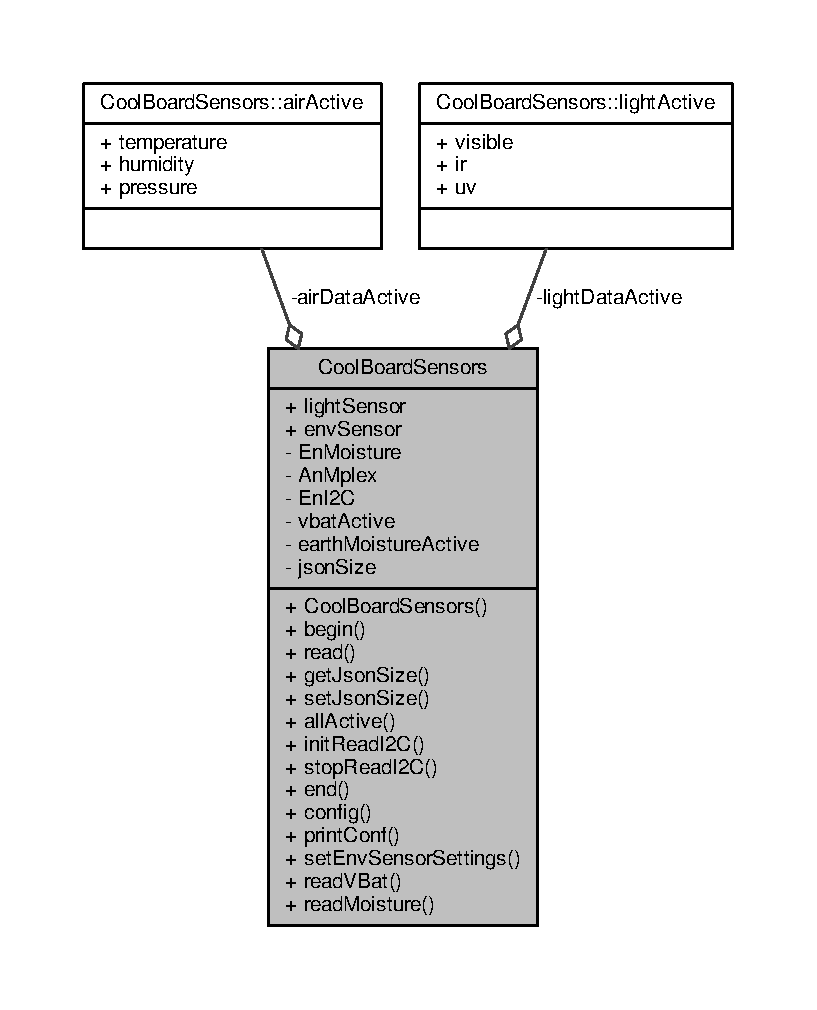
\includegraphics[width=350pt]{classCoolBoardSensors__coll__graph}
\end{center}
\end{figure}
\subsection*{Classes}
\begin{DoxyCompactItemize}
\item 
struct \hyperlink{structCoolBoardSensors_1_1airActive}{air\+Active}
\item 
struct \hyperlink{structCoolBoardSensors_1_1lightActive}{light\+Active}
\end{DoxyCompactItemize}
\subsection*{Public Member Functions}
\begin{DoxyCompactItemize}
\item 
\hyperlink{classCoolBoardSensors_a91ff2a02f5486f90cf2413a1cf8a9ed4}{Cool\+Board\+Sensors} ()
\item 
void \hyperlink{classCoolBoardSensors_a97095823ef7c8f5290812f1405b966b3}{begin} ()
\item 
String \hyperlink{classCoolBoardSensors_a91badb2539d91fda8679f2a597874c48}{read} ()
\item 
int \hyperlink{classCoolBoardSensors_ab82c2a1633768ccd12a589320fa31a14}{get\+Json\+Size} ()
\item 
void \hyperlink{classCoolBoardSensors_ab76e6dbd6efbcc25ff460535badd8d45}{set\+Json\+Size} (int \hyperlink{classCoolBoardSensors_a05a40dc80bfff14ffb830f549b876f8d}{json\+Size})
\item 
void \hyperlink{classCoolBoardSensors_aa432c5aac88f89c31a10766390f23e0b}{all\+Active} ()
\item 
void \hyperlink{classCoolBoardSensors_acad6a8418c66d36868caca23c844ecb6}{init\+Read\+I2C} ()
\item 
void \hyperlink{classCoolBoardSensors_ab67b900b9e5e7c18d52d2d9107ba171b}{stop\+Read\+I2C} ()
\item 
void \hyperlink{classCoolBoardSensors_a4902b69f6e628bd6557193758fdd2bae}{end} ()
\item 
bool \hyperlink{classCoolBoardSensors_a9a218895c5423375c33c08f2c56fb23a}{config} ()
\item 
void \hyperlink{classCoolBoardSensors_af6fd79505815b204c178617ecf54c873}{print\+Conf} ()
\item 
void \hyperlink{classCoolBoardSensors_a406307ffd70272282d91479c7ed8d66f}{set\+Env\+Sensor\+Settings} (uint8\+\_\+t comm\+Interface=I2\+C\+\_\+\+M\+O\+DE, uint8\+\_\+t I2\+C\+Address=0x76, uint8\+\_\+t run\+Mode=3, uint8\+\_\+t t\+Standby=0, uint8\+\_\+t filter=0, uint8\+\_\+t temp\+Over\+Sample=1, uint8\+\_\+t press\+Over\+Sample=1, uint8\+\_\+t humid\+Over\+Sample=1)
\item 
float \hyperlink{classCoolBoardSensors_a6944b6ea7bce8e2fce1b434acfd9d5f3}{read\+V\+Bat} ()
\item 
float \hyperlink{classCoolBoardSensors_a8761bff50373c485f4465c8db47d0633}{read\+Moisture} ()
\end{DoxyCompactItemize}
\subsection*{Public Attributes}
\begin{DoxyCompactItemize}
\item 
S\+I114X \hyperlink{classCoolBoardSensors_a3e397300fb707dd193e909a757bf6102}{light\+Sensor} = S\+I114X()
\item 
B\+M\+E280 \hyperlink{classCoolBoardSensors_a868e38985e9a2412829fa2790ca13e2e}{env\+Sensor}
\end{DoxyCompactItemize}
\subsection*{Private Attributes}
\begin{DoxyCompactItemize}
\item 
struct \hyperlink{structCoolBoardSensors_1_1lightActive}{Cool\+Board\+Sensors\+::light\+Active} \hyperlink{classCoolBoardSensors_ac4deb1cf41bac8b91c780c92fab00ba4}{light\+Data\+Active}
\item 
struct \hyperlink{structCoolBoardSensors_1_1airActive}{Cool\+Board\+Sensors\+::air\+Active} \hyperlink{classCoolBoardSensors_abff8dfeccb2f7689847bb64d5f1cd31e}{air\+Data\+Active}
\item 
const int \hyperlink{classCoolBoardSensors_a6177d02e14a057a2f171a2e930b5038d}{En\+Moisture} = 13
\item 
const int \hyperlink{classCoolBoardSensors_a12ef28b1046219e0aee10bf64e28c4a5}{An\+Mplex} = 12
\item 
const int \hyperlink{classCoolBoardSensors_aaa6b5dbf3a6633bffd9d204d961096dc}{En\+I2C} = 5
\item 
byte \hyperlink{classCoolBoardSensors_af5039ad760b0ff0aa7eee16c55e81702}{vbat\+Active}
\item 
byte \hyperlink{classCoolBoardSensors_a46dfddb8a12720e92cd2825ef09023c8}{earth\+Moisture\+Active}
\item 
int \hyperlink{classCoolBoardSensors_a05a40dc80bfff14ffb830f549b876f8d}{json\+Size}
\end{DoxyCompactItemize}


\subsection{Detailed Description}
This class handles the On-\/\+Board Sensors. 

Definition at line 24 of file Cool\+Board\+Sensors.\+h.



\subsection{Constructor \& Destructor Documentation}
\mbox{\Hypertarget{classCoolBoardSensors_a91ff2a02f5486f90cf2413a1cf8a9ed4}\label{classCoolBoardSensors_a91ff2a02f5486f90cf2413a1cf8a9ed4}} 
\index{Cool\+Board\+Sensors@{Cool\+Board\+Sensors}!Cool\+Board\+Sensors@{Cool\+Board\+Sensors}}
\index{Cool\+Board\+Sensors@{Cool\+Board\+Sensors}!Cool\+Board\+Sensors@{Cool\+Board\+Sensors}}
\subsubsection{\texorpdfstring{Cool\+Board\+Sensors()}{CoolBoardSensors()}}
{\footnotesize\ttfamily Cool\+Board\+Sensors\+::\+Cool\+Board\+Sensors (\begin{DoxyParamCaption}{ }\end{DoxyParamCaption})}

\hyperlink{classCoolBoardSensors_a91ff2a02f5486f90cf2413a1cf8a9ed4}{Cool\+Board\+Sensors\+::\+Cool\+Board\+Sensors()}\+: This Constructor is provided to start the I2C interface and Init the different used pins 

Definition at line 23 of file Cool\+Board\+Sensors.\+cpp.



References An\+Mplex, En\+I2C, and En\+Moisture.


\begin{DoxyCode}
24 \{
25     Wire.begin(2, 14);                       \textcolor{comment}{//I2C init Maybe change this to the CoolBoard?}
26 
27     pinMode(\hyperlink{classCoolBoardSensors_a12ef28b1046219e0aee10bf64e28c4a5}{AnMplex}, OUTPUT);                \textcolor{comment}{//Declare Analog Multiplexer OUTPUT}
28     pinMode(\hyperlink{classCoolBoardSensors_a6177d02e14a057a2f171a2e930b5038d}{EnMoisture}, OUTPUT);             \textcolor{comment}{//Declare Moisture enable Pin}
29     pinMode(\hyperlink{classCoolBoardSensors_aaa6b5dbf3a6633bffd9d204d961096dc}{EnI2C}, OUTPUT);           \textcolor{comment}{//Declare I2C Enable pin }
30 
31 
32 \}
\end{DoxyCode}


\subsection{Member Function Documentation}
\mbox{\Hypertarget{classCoolBoardSensors_aa432c5aac88f89c31a10766390f23e0b}\label{classCoolBoardSensors_aa432c5aac88f89c31a10766390f23e0b}} 
\index{Cool\+Board\+Sensors@{Cool\+Board\+Sensors}!all\+Active@{all\+Active}}
\index{all\+Active@{all\+Active}!Cool\+Board\+Sensors@{Cool\+Board\+Sensors}}
\subsubsection{\texorpdfstring{all\+Active()}{allActive()}}
{\footnotesize\ttfamily void Cool\+Board\+Sensors\+::all\+Active (\begin{DoxyParamCaption}{ }\end{DoxyParamCaption})}

\hyperlink{classCoolBoardSensors_aa432c5aac88f89c31a10766390f23e0b}{Cool\+Board\+Sensors\+::all\+Active()}\+: This method is provided to allow activation of all the sensor board sensors without passing by the configuration file/method 

Definition at line 62 of file Cool\+Board\+Sensors.\+cpp.



References air\+Data\+Active, earth\+Moisture\+Active, Cool\+Board\+Sensors\+::air\+Active\+::humidity, Cool\+Board\+Sensors\+::light\+Active\+::ir, light\+Data\+Active, Cool\+Board\+Sensors\+::air\+Active\+::pressure, Cool\+Board\+Sensors\+::air\+Active\+::temperature, Cool\+Board\+Sensors\+::light\+Active\+::uv, vbat\+Active, and Cool\+Board\+Sensors\+::light\+Active\+::visible.


\begin{DoxyCode}
63 \{
64     \hyperlink{classCoolBoardSensors_ac4deb1cf41bac8b91c780c92fab00ba4}{lightDataActive}.\hyperlink{structCoolBoardSensors_1_1lightActive_abcbba296b6a95e67c0cd2555d9dd50c7}{visible}=1;
65     \hyperlink{classCoolBoardSensors_ac4deb1cf41bac8b91c780c92fab00ba4}{lightDataActive}.\hyperlink{structCoolBoardSensors_1_1lightActive_a67700895349b95ceb263f1a6da756315}{ir}=1;
66     \hyperlink{classCoolBoardSensors_ac4deb1cf41bac8b91c780c92fab00ba4}{lightDataActive}.\hyperlink{structCoolBoardSensors_1_1lightActive_a949a7aaf5166d981de8fe0fd93da20d6}{uv}=1;  
67 
68     \hyperlink{classCoolBoardSensors_abff8dfeccb2f7689847bb64d5f1cd31e}{airDataActive}.\hyperlink{structCoolBoardSensors_1_1airActive_a9a6633c426b0508e30ebc1832ec6d745}{temperature}=1;
69     \hyperlink{classCoolBoardSensors_abff8dfeccb2f7689847bb64d5f1cd31e}{airDataActive}.\hyperlink{structCoolBoardSensors_1_1airActive_ae5740445054b27415e22f450576accb7}{humidity}=1;
70     \hyperlink{classCoolBoardSensors_abff8dfeccb2f7689847bb64d5f1cd31e}{airDataActive}.\hyperlink{structCoolBoardSensors_1_1airActive_ab200826a70d1dc9945f5efb6b9c732ed}{pressure}=1;
71 
72 
73     \hyperlink{classCoolBoardSensors_af5039ad760b0ff0aa7eee16c55e81702}{vbatActive}=1;
74     \hyperlink{classCoolBoardSensors_a46dfddb8a12720e92cd2825ef09023c8}{earthMoistureActive}=1;
75 
76 
77 \}
\end{DoxyCode}
\mbox{\Hypertarget{classCoolBoardSensors_a97095823ef7c8f5290812f1405b966b3}\label{classCoolBoardSensors_a97095823ef7c8f5290812f1405b966b3}} 
\index{Cool\+Board\+Sensors@{Cool\+Board\+Sensors}!begin@{begin}}
\index{begin@{begin}!Cool\+Board\+Sensors@{Cool\+Board\+Sensors}}
\subsubsection{\texorpdfstring{begin()}{begin()}}
{\footnotesize\ttfamily void Cool\+Board\+Sensors\+::begin (\begin{DoxyParamCaption}{ }\end{DoxyParamCaption})}

\hyperlink{classCoolBoardSensors_a97095823ef7c8f5290812f1405b966b3}{Cool\+Board\+Sensors\+::begin()}\+: This method is provided to start the sensors that are on the sensor board 

Definition at line 85 of file Cool\+Board\+Sensors.\+cpp.



References env\+Sensor, init\+Read\+I2\+C(), light\+Sensor, and set\+Env\+Sensor\+Settings().



Referenced by Cool\+Board\+::begin().


\begin{DoxyCode}
86 \{       
87     \hyperlink{classCoolBoardSensors_acad6a8418c66d36868caca23c844ecb6}{initReadI2C}();
88 
89     \textcolor{keywordflow}{while} (!\hyperlink{classCoolBoardSensors_a3e397300fb707dd193e909a757bf6102}{lightSensor}.Begin()) \{
90       Serial.println(\textcolor{stringliteral}{"Si1145 is not ready!  1 second"});
91       delay(1000);
92     \}
93      
94     this->\hyperlink{classCoolBoardSensors_a406307ffd70272282d91479c7ed8d66f}{setEnvSensorSettings}();
95     delay(10);  \textcolor{comment}{//Make sure sensor had enough time to turn on. BME280 requires 2ms to start up.}
96     this->\hyperlink{classCoolBoardSensors_a868e38985e9a2412829fa2790ca13e2e}{envSensor}.begin();
97     delay(10);  \textcolor{comment}{//Make sure sensor had enough time to turn on. BME280 requires 2ms to start up.}
98     Serial.println(\hyperlink{classCoolBoardSensors_a868e38985e9a2412829fa2790ca13e2e}{envSensor}.begin(), HEX);
99 
100 
101 \}
\end{DoxyCode}
Here is the call graph for this function\+:\nopagebreak
\begin{figure}[H]
\begin{center}
\leavevmode
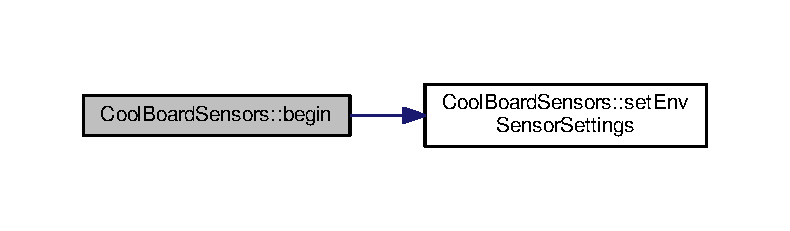
\includegraphics[width=350pt]{classCoolBoardSensors_a97095823ef7c8f5290812f1405b966b3_cgraph}
\end{center}
\end{figure}
Here is the caller graph for this function\+:\nopagebreak
\begin{figure}[H]
\begin{center}
\leavevmode
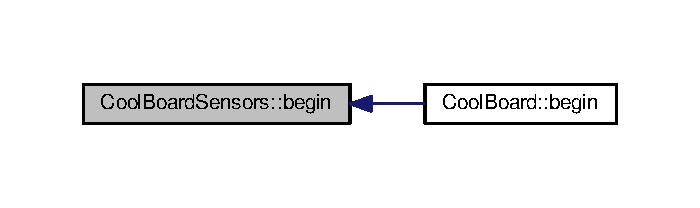
\includegraphics[width=336pt]{classCoolBoardSensors_a97095823ef7c8f5290812f1405b966b3_icgraph}
\end{center}
\end{figure}
\mbox{\Hypertarget{classCoolBoardSensors_a9a218895c5423375c33c08f2c56fb23a}\label{classCoolBoardSensors_a9a218895c5423375c33c08f2c56fb23a}} 
\index{Cool\+Board\+Sensors@{Cool\+Board\+Sensors}!config@{config}}
\index{config@{config}!Cool\+Board\+Sensors@{Cool\+Board\+Sensors}}
\subsubsection{\texorpdfstring{config()}{config()}}
{\footnotesize\ttfamily bool Cool\+Board\+Sensors\+::config (\begin{DoxyParamCaption}{ }\end{DoxyParamCaption})}

\hyperlink{classCoolBoardSensors_a9a218895c5423375c33c08f2c56fb23a}{Cool\+Board\+Sensors\+::config()}\+: This method is provided to configure the sensor board \+: -\/activate 1 -\/deactivate 0

\begin{DoxyReturn}{Returns}
true if configuration is successful, false otherwise 
\end{DoxyReturn}


Definition at line 222 of file Cool\+Board\+Sensors.\+cpp.



References air\+Data\+Active, earth\+Moisture\+Active, Cool\+Board\+Sensors\+::air\+Active\+::humidity, Cool\+Board\+Sensors\+::light\+Active\+::ir, json\+Size, light\+Data\+Active, Cool\+Board\+Sensors\+::air\+Active\+::pressure, Cool\+Board\+Sensors\+::air\+Active\+::temperature, Cool\+Board\+Sensors\+::light\+Active\+::uv, vbat\+Active, and Cool\+Board\+Sensors\+::light\+Active\+::visible.



Referenced by Cool\+Board\+::begin(), and Cool\+Board\+::update().


\begin{DoxyCode}
223 \{
224     \textcolor{comment}{//read config file}
225     \textcolor{comment}{//update data}
226     File coolBoardSensorsConfig = SPIFFS.open(\textcolor{stringliteral}{"/coolBoardSensorsConfig.json"}, \textcolor{stringliteral}{"r"});
227 
228     \textcolor{keywordflow}{if} (!coolBoardSensorsConfig) 
229     \{
230         \textcolor{keywordflow}{return}(\textcolor{keyword}{false});
231     \}
232     \textcolor{keywordflow}{else}
233     \{
234         \textcolor{keywordtype}{size\_t} size = coolBoardSensorsConfig.size();
235         \textcolor{comment}{// Allocate a buffer to store contents of the file.}
236         std::unique\_ptr<char[]> buf(\textcolor{keyword}{new} \textcolor{keywordtype}{char}[size]);
237 
238         coolBoardSensorsConfig.readBytes(buf.get(), size);
239         DynamicJsonBuffer jsonBuffer;
240         JsonObject& json = jsonBuffer.parseObject(buf.get());
241         \textcolor{keywordflow}{if} (!json.success()) 
242         \{
243               \textcolor{keywordflow}{return}(\textcolor{keyword}{false});
244         \} 
245         \textcolor{keywordflow}{else}
246         \{     
247             \textcolor{keywordflow}{if}(json[\textcolor{stringliteral}{"jsonSize"}].success() )
248             \{
249                 this->\hyperlink{classCoolBoardSensors_a05a40dc80bfff14ffb830f549b876f8d}{jsonSize} = json[\textcolor{stringliteral}{"jsonSize"}]; 
250             \}
251             \textcolor{keywordflow}{else}
252             \{
253                 this->\hyperlink{classCoolBoardSensors_a05a40dc80bfff14ffb830f549b876f8d}{jsonSize}=this->\hyperlink{classCoolBoardSensors_a05a40dc80bfff14ffb830f549b876f8d}{jsonSize};          
254             \}
255             json[\textcolor{stringliteral}{"jsonSize"}]=this->\hyperlink{classCoolBoardSensors_a05a40dc80bfff14ffb830f549b876f8d}{jsonSize};
256 
257             
258             \textcolor{keywordflow}{if}(json[\textcolor{stringliteral}{"BME280"}][\textcolor{stringliteral}{"temperature"}].success() )
259             \{           
260                 this->\hyperlink{classCoolBoardSensors_abff8dfeccb2f7689847bb64d5f1cd31e}{airDataActive}.\hyperlink{structCoolBoardSensors_1_1airActive_a9a6633c426b0508e30ebc1832ec6d745}{temperature}=json[\textcolor{stringliteral}{"BME280"}][\textcolor{stringliteral}{"temperature"}];
261             \}
262             \textcolor{keywordflow}{else}
263             \{
264                 this->\hyperlink{classCoolBoardSensors_abff8dfeccb2f7689847bb64d5f1cd31e}{airDataActive}.\hyperlink{structCoolBoardSensors_1_1airActive_a9a6633c426b0508e30ebc1832ec6d745}{temperature}=this->
      \hyperlink{classCoolBoardSensors_abff8dfeccb2f7689847bb64d5f1cd31e}{airDataActive}.\hyperlink{structCoolBoardSensors_1_1airActive_a9a6633c426b0508e30ebc1832ec6d745}{temperature};          
265             \}
266             json[\textcolor{stringliteral}{"BME280"}][\textcolor{stringliteral}{"temperature"}]=this->\hyperlink{classCoolBoardSensors_abff8dfeccb2f7689847bb64d5f1cd31e}{airDataActive}.
      \hyperlink{structCoolBoardSensors_1_1airActive_a9a6633c426b0508e30ebc1832ec6d745}{temperature};
267             
268             
269             \textcolor{keywordflow}{if}(json[\textcolor{stringliteral}{"BME280"}][\textcolor{stringliteral}{"humidity"}].success() )
270             \{           
271             
272                 this->\hyperlink{classCoolBoardSensors_abff8dfeccb2f7689847bb64d5f1cd31e}{airDataActive}.\hyperlink{structCoolBoardSensors_1_1airActive_ae5740445054b27415e22f450576accb7}{humidity}=json[\textcolor{stringliteral}{"BME280"}][\textcolor{stringliteral}{"humidity"}];
273             \}
274             \textcolor{keywordflow}{else}
275             \{
276                 this->\hyperlink{classCoolBoardSensors_abff8dfeccb2f7689847bb64d5f1cd31e}{airDataActive}.\hyperlink{structCoolBoardSensors_1_1airActive_ae5740445054b27415e22f450576accb7}{humidity}=this->
      \hyperlink{classCoolBoardSensors_abff8dfeccb2f7689847bb64d5f1cd31e}{airDataActive}.\hyperlink{structCoolBoardSensors_1_1airActive_ae5740445054b27415e22f450576accb7}{humidity};
277             \}
278             json[\textcolor{stringliteral}{"BME280"}][\textcolor{stringliteral}{"humidity"}]=this->\hyperlink{classCoolBoardSensors_abff8dfeccb2f7689847bb64d5f1cd31e}{airDataActive}.\hyperlink{structCoolBoardSensors_1_1airActive_ae5740445054b27415e22f450576accb7}{humidity};
279             
280             
281             \textcolor{keywordflow}{if}(json[\textcolor{stringliteral}{"BME280"}][\textcolor{stringliteral}{"pressure"}].success() )
282             \{
283                 this->\hyperlink{classCoolBoardSensors_abff8dfeccb2f7689847bb64d5f1cd31e}{airDataActive}.\hyperlink{structCoolBoardSensors_1_1airActive_ab200826a70d1dc9945f5efb6b9c732ed}{pressure}=json[\textcolor{stringliteral}{"BME280"}][\textcolor{stringliteral}{"pressure"}];
284             \}
285             \textcolor{keywordflow}{else}
286             \{
287                 this->\hyperlink{classCoolBoardSensors_abff8dfeccb2f7689847bb64d5f1cd31e}{airDataActive}.\hyperlink{structCoolBoardSensors_1_1airActive_ab200826a70d1dc9945f5efb6b9c732ed}{pressure}=this->
      \hyperlink{classCoolBoardSensors_abff8dfeccb2f7689847bb64d5f1cd31e}{airDataActive}.\hyperlink{structCoolBoardSensors_1_1airActive_ab200826a70d1dc9945f5efb6b9c732ed}{pressure};
288             \}
289             json[\textcolor{stringliteral}{"BME280"}][\textcolor{stringliteral}{"pressure"}]=this->\hyperlink{classCoolBoardSensors_abff8dfeccb2f7689847bb64d5f1cd31e}{airDataActive}.\hyperlink{structCoolBoardSensors_1_1airActive_ab200826a70d1dc9945f5efb6b9c732ed}{pressure};
290 
291             
292             \textcolor{keywordflow}{if}(json[\textcolor{stringliteral}{"SI114X"}][\textcolor{stringliteral}{"visible"}].success() )
293             \{
294                 this->\hyperlink{classCoolBoardSensors_ac4deb1cf41bac8b91c780c92fab00ba4}{lightDataActive}.\hyperlink{structCoolBoardSensors_1_1lightActive_abcbba296b6a95e67c0cd2555d9dd50c7}{visible}=json[\textcolor{stringliteral}{"SI114X"}][\textcolor{stringliteral}{"visible"}];
295             \}
296             \textcolor{keywordflow}{else}
297             \{
298                 this->\hyperlink{classCoolBoardSensors_ac4deb1cf41bac8b91c780c92fab00ba4}{lightDataActive}.\hyperlink{structCoolBoardSensors_1_1lightActive_abcbba296b6a95e67c0cd2555d9dd50c7}{visible}=this->
      \hyperlink{classCoolBoardSensors_ac4deb1cf41bac8b91c780c92fab00ba4}{lightDataActive}.\hyperlink{structCoolBoardSensors_1_1lightActive_abcbba296b6a95e67c0cd2555d9dd50c7}{visible};
299             \}
300             json[\textcolor{stringliteral}{"SI114X"}][\textcolor{stringliteral}{"visible"}]=this->\hyperlink{classCoolBoardSensors_ac4deb1cf41bac8b91c780c92fab00ba4}{lightDataActive}.
      \hyperlink{structCoolBoardSensors_1_1lightActive_abcbba296b6a95e67c0cd2555d9dd50c7}{visible};
301             
302             
303             \textcolor{keywordflow}{if}(json[\textcolor{stringliteral}{"SI114X"}][\textcolor{stringliteral}{"ir"}].success() )
304             \{           
305                 this->\hyperlink{classCoolBoardSensors_ac4deb1cf41bac8b91c780c92fab00ba4}{lightDataActive}.\hyperlink{structCoolBoardSensors_1_1lightActive_a67700895349b95ceb263f1a6da756315}{ir}=json[\textcolor{stringliteral}{"SI114X"}][\textcolor{stringliteral}{"ir"}];
306             \}
307             \textcolor{keywordflow}{else}
308             \{
309                 this->\hyperlink{classCoolBoardSensors_ac4deb1cf41bac8b91c780c92fab00ba4}{lightDataActive}.\hyperlink{structCoolBoardSensors_1_1lightActive_a67700895349b95ceb263f1a6da756315}{ir}=this->\hyperlink{classCoolBoardSensors_ac4deb1cf41bac8b91c780c92fab00ba4}{lightDataActive}.
      \hyperlink{structCoolBoardSensors_1_1lightActive_a67700895349b95ceb263f1a6da756315}{ir};
310             \}
311             json[\textcolor{stringliteral}{"SI114X"}][\textcolor{stringliteral}{"ir"}]=this->\hyperlink{classCoolBoardSensors_ac4deb1cf41bac8b91c780c92fab00ba4}{lightDataActive}.\hyperlink{structCoolBoardSensors_1_1lightActive_a67700895349b95ceb263f1a6da756315}{ir};
312 
313             
314             \textcolor{keywordflow}{if}(json[\textcolor{stringliteral}{"SI114X"}][\textcolor{stringliteral}{"uv"}].success() )         
315             \{           
316                 this->\hyperlink{classCoolBoardSensors_ac4deb1cf41bac8b91c780c92fab00ba4}{lightDataActive}.\hyperlink{structCoolBoardSensors_1_1lightActive_a949a7aaf5166d981de8fe0fd93da20d6}{uv}=json[\textcolor{stringliteral}{"SI114X"}][\textcolor{stringliteral}{"uv"}];
317             \}
318             \textcolor{keywordflow}{else}
319             \{
320                 this->\hyperlink{classCoolBoardSensors_ac4deb1cf41bac8b91c780c92fab00ba4}{lightDataActive}.\hyperlink{structCoolBoardSensors_1_1lightActive_a949a7aaf5166d981de8fe0fd93da20d6}{uv}=this->\hyperlink{classCoolBoardSensors_ac4deb1cf41bac8b91c780c92fab00ba4}{lightDataActive}.
      \hyperlink{structCoolBoardSensors_1_1lightActive_a949a7aaf5166d981de8fe0fd93da20d6}{uv};
321             \}
322             json[\textcolor{stringliteral}{"SI114X"}][\textcolor{stringliteral}{"uv"}]=this->\hyperlink{classCoolBoardSensors_ac4deb1cf41bac8b91c780c92fab00ba4}{lightDataActive}.\hyperlink{structCoolBoardSensors_1_1lightActive_a949a7aaf5166d981de8fe0fd93da20d6}{uv};
323 
324 
325             \textcolor{keywordflow}{if}(json[\textcolor{stringliteral}{"vbat"}].success() )
326             \{
327                 this->\hyperlink{classCoolBoardSensors_af5039ad760b0ff0aa7eee16c55e81702}{vbatActive}=json[\textcolor{stringliteral}{"vbat"}];
328             \}
329             \textcolor{keywordflow}{else}
330             \{
331                 this->\hyperlink{classCoolBoardSensors_af5039ad760b0ff0aa7eee16c55e81702}{vbatActive}=this->\hyperlink{classCoolBoardSensors_af5039ad760b0ff0aa7eee16c55e81702}{vbatActive};
332             \}
333             json[\textcolor{stringliteral}{"vbat"}]=this->\hyperlink{classCoolBoardSensors_af5039ad760b0ff0aa7eee16c55e81702}{vbatActive};
334 
335             
336             \textcolor{keywordflow}{if}(json[\textcolor{stringliteral}{"soilMoisture"}].success() )
337             \{           
338                 this->\hyperlink{classCoolBoardSensors_a46dfddb8a12720e92cd2825ef09023c8}{earthMoistureActive}= json[\textcolor{stringliteral}{"soilMoisture"}];
339             \}
340             \textcolor{keywordflow}{else}
341             \{
342                 this->\hyperlink{classCoolBoardSensors_a46dfddb8a12720e92cd2825ef09023c8}{earthMoistureActive}=this->
      \hyperlink{classCoolBoardSensors_a46dfddb8a12720e92cd2825ef09023c8}{earthMoistureActive};
343             \}
344             json[\textcolor{stringliteral}{"soilMoisture"}]=this->\hyperlink{classCoolBoardSensors_a46dfddb8a12720e92cd2825ef09023c8}{earthMoistureActive};
345 
346             coolBoardSensorsConfig.close();         
347             coolBoardSensorsConfig = SPIFFS.open(\textcolor{stringliteral}{"/coolBoardSensorsConfig.json"}, \textcolor{stringliteral}{"w"});          
348             \textcolor{keywordflow}{if}(!coolBoardSensorsConfig)
349             \{
350                 \textcolor{keywordflow}{return}(\textcolor{keyword}{false});          
351             \}  
352 
353             json.printTo(coolBoardSensorsConfig);
354             coolBoardSensorsConfig.close();         
355             
356               \textcolor{keywordflow}{return}(\textcolor{keyword}{true}); 
357         \}
358     \}   
359 
360 \}
\end{DoxyCode}
Here is the caller graph for this function\+:\nopagebreak
\begin{figure}[H]
\begin{center}
\leavevmode
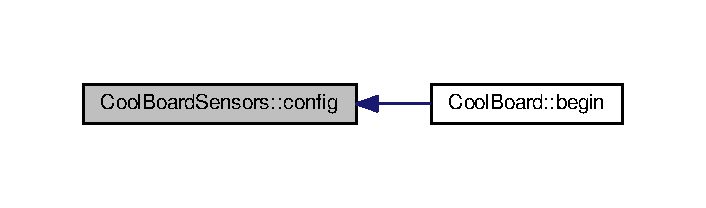
\includegraphics[width=350pt]{classCoolBoardSensors_a9a218895c5423375c33c08f2c56fb23a_icgraph}
\end{center}
\end{figure}
\mbox{\Hypertarget{classCoolBoardSensors_a4902b69f6e628bd6557193758fdd2bae}\label{classCoolBoardSensors_a4902b69f6e628bd6557193758fdd2bae}} 
\index{Cool\+Board\+Sensors@{Cool\+Board\+Sensors}!end@{end}}
\index{end@{end}!Cool\+Board\+Sensors@{Cool\+Board\+Sensors}}
\subsubsection{\texorpdfstring{end()}{end()}}
{\footnotesize\ttfamily void Cool\+Board\+Sensors\+::end (\begin{DoxyParamCaption}{ }\end{DoxyParamCaption})}

\hyperlink{classCoolBoardSensors_a4902b69f6e628bd6557193758fdd2bae}{Cool\+Board\+Sensors\+::end()}\+: This method is provided to end the sensors on the sensor board 

Definition at line 108 of file Cool\+Board\+Sensors.\+cpp.



References light\+Sensor.


\begin{DoxyCode}
109 \{
110 
111     \hyperlink{classCoolBoardSensors_a3e397300fb707dd193e909a757bf6102}{lightSensor}.DeInit();
112 
113 \}
\end{DoxyCode}
\mbox{\Hypertarget{classCoolBoardSensors_ab82c2a1633768ccd12a589320fa31a14}\label{classCoolBoardSensors_ab82c2a1633768ccd12a589320fa31a14}} 
\index{Cool\+Board\+Sensors@{Cool\+Board\+Sensors}!get\+Json\+Size@{get\+Json\+Size}}
\index{get\+Json\+Size@{get\+Json\+Size}!Cool\+Board\+Sensors@{Cool\+Board\+Sensors}}
\subsubsection{\texorpdfstring{get\+Json\+Size()}{getJsonSize()}}
{\footnotesize\ttfamily int Cool\+Board\+Sensors\+::get\+Json\+Size (\begin{DoxyParamCaption}{ }\end{DoxyParamCaption})}

\hyperlink{classCoolBoardSensors_ab82c2a1633768ccd12a589320fa31a14}{Cool\+Board\+Sensors\+::get\+Json\+Size()}\+: This method is provided to get the sensor board answer size

\begin{DoxyReturn}{Returns}
json data size 
\end{DoxyReturn}


Definition at line 41 of file Cool\+Board\+Sensors.\+cpp.



References json\+Size.


\begin{DoxyCode}
42 \{
43     \textcolor{keywordflow}{return}(this->\hyperlink{classCoolBoardSensors_a05a40dc80bfff14ffb830f549b876f8d}{jsonSize} );
44 \}
\end{DoxyCode}
\mbox{\Hypertarget{classCoolBoardSensors_acad6a8418c66d36868caca23c844ecb6}\label{classCoolBoardSensors_acad6a8418c66d36868caca23c844ecb6}} 
\index{Cool\+Board\+Sensors@{Cool\+Board\+Sensors}!init\+Read\+I2C@{init\+Read\+I2C}}
\index{init\+Read\+I2C@{init\+Read\+I2C}!Cool\+Board\+Sensors@{Cool\+Board\+Sensors}}
\subsubsection{\texorpdfstring{init\+Read\+I2\+C()}{initReadI2C()}}
{\footnotesize\ttfamily void Cool\+Board\+Sensors\+::init\+Read\+I2C (\begin{DoxyParamCaption}{ }\end{DoxyParamCaption})}

\hyperlink{classCoolBoardSensors_acad6a8418c66d36868caca23c844ecb6}{Cool\+Board\+Sensors\+::init\+Read\+I2\+C()}\+: This method is provided to enable the I2C Interface on the sensor board. 

Definition at line 193 of file Cool\+Board\+Sensors.\+cpp.



References En\+I2C.



Referenced by begin(), and read().


\begin{DoxyCode}
194 \{
195   
196     digitalWrite(\hyperlink{classCoolBoardSensors_aaa6b5dbf3a6633bffd9d204d961096dc}{EnI2C},HIGH);\textcolor{comment}{//HIGH= I2C Enable}
197 
198 \}
\end{DoxyCode}
Here is the caller graph for this function\+:
\nopagebreak
\begin{figure}[H]
\begin{center}
\leavevmode
\includegraphics[width=350pt]{classCoolBoardSensors_acad6a8418c66d36868caca23c844ecb6_icgraph}
\end{center}
\end{figure}
\mbox{\Hypertarget{classCoolBoardSensors_af6fd79505815b204c178617ecf54c873}\label{classCoolBoardSensors_af6fd79505815b204c178617ecf54c873}} 
\index{Cool\+Board\+Sensors@{Cool\+Board\+Sensors}!print\+Conf@{print\+Conf}}
\index{print\+Conf@{print\+Conf}!Cool\+Board\+Sensors@{Cool\+Board\+Sensors}}
\subsubsection{\texorpdfstring{print\+Conf()}{printConf()}}
{\footnotesize\ttfamily void Cool\+Board\+Sensors\+::print\+Conf (\begin{DoxyParamCaption}{ }\end{DoxyParamCaption})}

\hyperlink{classCoolBoardSensors_af6fd79505815b204c178617ecf54c873}{Cool\+Board\+Sensors\+::print\+Conf()}\+: This method is provided to print the configuration to the Serial Monitor 

Definition at line 368 of file Cool\+Board\+Sensors.\+cpp.



References air\+Data\+Active, earth\+Moisture\+Active, Cool\+Board\+Sensors\+::air\+Active\+::humidity, Cool\+Board\+Sensors\+::light\+Active\+::ir, json\+Size, light\+Data\+Active, Cool\+Board\+Sensors\+::air\+Active\+::pressure, Cool\+Board\+Sensors\+::air\+Active\+::temperature, Cool\+Board\+Sensors\+::light\+Active\+::uv, vbat\+Active, and Cool\+Board\+Sensors\+::light\+Active\+::visible.



Referenced by Cool\+Board\+::begin().


\begin{DoxyCode}
369 \{
370     Serial.println(\textcolor{stringliteral}{"Sensors Conf "});
371     Serial.println(\hyperlink{classCoolBoardSensors_a05a40dc80bfff14ffb830f549b876f8d}{jsonSize});
372     Serial.println(\hyperlink{classCoolBoardSensors_abff8dfeccb2f7689847bb64d5f1cd31e}{airDataActive}.\hyperlink{structCoolBoardSensors_1_1airActive_a9a6633c426b0508e30ebc1832ec6d745}{temperature});
373     Serial.println(\hyperlink{classCoolBoardSensors_abff8dfeccb2f7689847bb64d5f1cd31e}{airDataActive}.\hyperlink{structCoolBoardSensors_1_1airActive_ae5740445054b27415e22f450576accb7}{humidity});
374     Serial.println(\hyperlink{classCoolBoardSensors_abff8dfeccb2f7689847bb64d5f1cd31e}{airDataActive}.\hyperlink{structCoolBoardSensors_1_1airActive_ab200826a70d1dc9945f5efb6b9c732ed}{pressure});
375 
376     Serial.println(\hyperlink{classCoolBoardSensors_ac4deb1cf41bac8b91c780c92fab00ba4}{lightDataActive}.\hyperlink{structCoolBoardSensors_1_1lightActive_abcbba296b6a95e67c0cd2555d9dd50c7}{visible});
377     Serial.println(\hyperlink{classCoolBoardSensors_ac4deb1cf41bac8b91c780c92fab00ba4}{lightDataActive}.\hyperlink{structCoolBoardSensors_1_1lightActive_a67700895349b95ceb263f1a6da756315}{ir});
378     Serial.println(\hyperlink{classCoolBoardSensors_ac4deb1cf41bac8b91c780c92fab00ba4}{lightDataActive}.\hyperlink{structCoolBoardSensors_1_1lightActive_a949a7aaf5166d981de8fe0fd93da20d6}{uv});
379     Serial.println(\hyperlink{classCoolBoardSensors_af5039ad760b0ff0aa7eee16c55e81702}{vbatActive});
380     Serial.println(\hyperlink{classCoolBoardSensors_a46dfddb8a12720e92cd2825ef09023c8}{earthMoistureActive});
381     Serial.println(\textcolor{stringliteral}{" "});
382 \}
\end{DoxyCode}
Here is the caller graph for this function\+:
\nopagebreak
\begin{figure}[H]
\begin{center}
\leavevmode
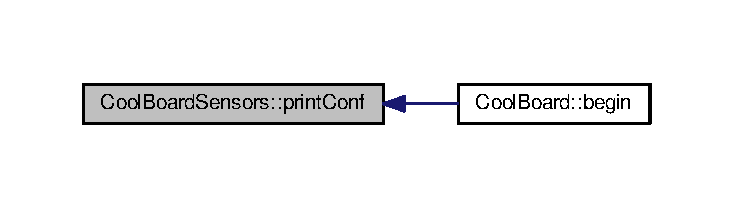
\includegraphics[width=350pt]{classCoolBoardSensors_af6fd79505815b204c178617ecf54c873_icgraph}
\end{center}
\end{figure}
\mbox{\Hypertarget{classCoolBoardSensors_a91badb2539d91fda8679f2a597874c48}\label{classCoolBoardSensors_a91badb2539d91fda8679f2a597874c48}} 
\index{Cool\+Board\+Sensors@{Cool\+Board\+Sensors}!read@{read}}
\index{read@{read}!Cool\+Board\+Sensors@{Cool\+Board\+Sensors}}
\subsubsection{\texorpdfstring{read()}{read()}}
{\footnotesize\ttfamily String Cool\+Board\+Sensors\+::read (\begin{DoxyParamCaption}{ }\end{DoxyParamCaption})}

\hyperlink{classCoolBoardSensors_a91badb2539d91fda8679f2a597874c48}{Cool\+Board\+Sensors\+::read()}\+: This method is provided to return the data read by the sensor board

\begin{DoxyReturn}{Returns}
a json string containing the sensors data 
\end{DoxyReturn}


Definition at line 123 of file Cool\+Board\+Sensors.\+cpp.



References air\+Data\+Active, earth\+Moisture\+Active, env\+Sensor, Cool\+Board\+Sensors\+::air\+Active\+::humidity, init\+Read\+I2\+C(), Cool\+Board\+Sensors\+::light\+Active\+::ir, json\+Size, light\+Data\+Active, light\+Sensor, Cool\+Board\+Sensors\+::air\+Active\+::pressure, read\+Moisture(), read\+V\+Bat(), Cool\+Board\+Sensors\+::air\+Active\+::temperature, Cool\+Board\+Sensors\+::light\+Active\+::uv, vbat\+Active, and Cool\+Board\+Sensors\+::light\+Active\+::visible.



Referenced by Cool\+Board\+::read\+Sensors().


\begin{DoxyCode}
124 \{
125     String data;
126     DynamicJsonBuffer  jsonBuffer(\hyperlink{classCoolBoardSensors_a05a40dc80bfff14ffb830f549b876f8d}{jsonSize}) ;
127     JsonObject& root = jsonBuffer.createObject();
128     
129     \hyperlink{classCoolBoardSensors_acad6a8418c66d36868caca23c844ecb6}{initReadI2C}();
130     delay(100);
131     \textcolor{comment}{//light data}
132     \textcolor{keywordflow}{if}(\hyperlink{classCoolBoardSensors_ac4deb1cf41bac8b91c780c92fab00ba4}{lightDataActive}.\hyperlink{structCoolBoardSensors_1_1lightActive_abcbba296b6a95e67c0cd2555d9dd50c7}{visible})
133     \{
134 
135         root[\textcolor{stringliteral}{"visibleLight"}] =\hyperlink{classCoolBoardSensors_a3e397300fb707dd193e909a757bf6102}{lightSensor}.ReadVisible() ;
136     \}
137     
138     \textcolor{keywordflow}{if}(\hyperlink{classCoolBoardSensors_ac4deb1cf41bac8b91c780c92fab00ba4}{lightDataActive}.\hyperlink{structCoolBoardSensors_1_1lightActive_a67700895349b95ceb263f1a6da756315}{ir})
139     \{
140         root[\textcolor{stringliteral}{"infraRed"}] = \hyperlink{classCoolBoardSensors_a3e397300fb707dd193e909a757bf6102}{lightSensor}.ReadIR();
141     \}
142 
143     \textcolor{keywordflow}{if}(\hyperlink{classCoolBoardSensors_ac4deb1cf41bac8b91c780c92fab00ba4}{lightDataActive}.\hyperlink{structCoolBoardSensors_1_1lightActive_a949a7aaf5166d981de8fe0fd93da20d6}{uv})
144     \{
145         \textcolor{keywordtype}{float} tempUV = (float)\hyperlink{classCoolBoardSensors_a3e397300fb707dd193e909a757bf6102}{lightSensor}.ReadUV()/100 ;
146         root[\textcolor{stringliteral}{"ultraViolet"}] = tempUV;
147     \}
148     
149     \textcolor{comment}{//BME280 data}
150     \textcolor{keywordflow}{if}(\hyperlink{classCoolBoardSensors_abff8dfeccb2f7689847bb64d5f1cd31e}{airDataActive}.\hyperlink{structCoolBoardSensors_1_1airActive_ab200826a70d1dc9945f5efb6b9c732ed}{pressure}) 
151     \{
152         root[\textcolor{stringliteral}{"Pressure"}] =\hyperlink{classCoolBoardSensors_a868e38985e9a2412829fa2790ca13e2e}{envSensor}.readFloatPressure();
153     \}
154     
155         
156     \textcolor{keywordflow}{if}(\hyperlink{classCoolBoardSensors_abff8dfeccb2f7689847bb64d5f1cd31e}{airDataActive}.\hyperlink{structCoolBoardSensors_1_1airActive_ae5740445054b27415e22f450576accb7}{humidity}) 
157     \{   
158         root[\textcolor{stringliteral}{"Humidity"}] =\hyperlink{classCoolBoardSensors_a868e38985e9a2412829fa2790ca13e2e}{envSensor}.readFloatHumidity() ;
159     \}   
160     
161     \textcolor{keywordflow}{if}(\hyperlink{classCoolBoardSensors_abff8dfeccb2f7689847bb64d5f1cd31e}{airDataActive}.\hyperlink{structCoolBoardSensors_1_1airActive_a9a6633c426b0508e30ebc1832ec6d745}{temperature})
162     \{
163         root[\textcolor{stringliteral}{"Temperature"}]=\hyperlink{classCoolBoardSensors_a868e38985e9a2412829fa2790ca13e2e}{envSensor}.readTempC();
164     \}
165     
166     \textcolor{comment}{//Vbat}
167     \textcolor{keywordflow}{if}(\hyperlink{classCoolBoardSensors_af5039ad760b0ff0aa7eee16c55e81702}{vbatActive})    
168     \{   
169         root[\textcolor{stringliteral}{"Vbat"}]=this->\hyperlink{classCoolBoardSensors_a6944b6ea7bce8e2fce1b434acfd9d5f3}{readVBat}();
170     \}
171     
172     \textcolor{comment}{//earth Moisture}
173     \textcolor{keywordflow}{if}(\hyperlink{classCoolBoardSensors_a46dfddb8a12720e92cd2825ef09023c8}{earthMoistureActive})
174     \{   
175         root[\textcolor{stringliteral}{"soilMoisture"}]=this->\hyperlink{classCoolBoardSensors_a8761bff50373c485f4465c8db47d0633}{readMoisture}();
176     \}
177     
178     
179     root.printTo(data);
180     
181 
182 
183     \textcolor{keywordflow}{return}(data);
184     
185 
186 \}
\end{DoxyCode}
Here is the call graph for this function\+:
\nopagebreak
\begin{figure}[H]
\begin{center}
\leavevmode
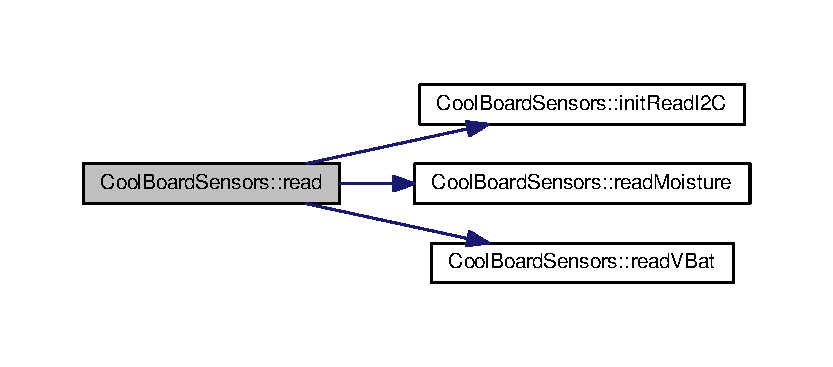
\includegraphics[width=350pt]{classCoolBoardSensors_a91badb2539d91fda8679f2a597874c48_cgraph}
\end{center}
\end{figure}
Here is the caller graph for this function\+:
\nopagebreak
\begin{figure}[H]
\begin{center}
\leavevmode
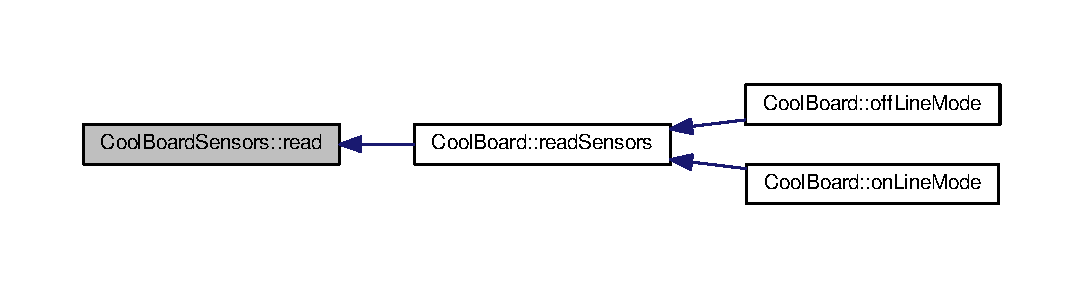
\includegraphics[width=350pt]{classCoolBoardSensors_a91badb2539d91fda8679f2a597874c48_icgraph}
\end{center}
\end{figure}
\mbox{\Hypertarget{classCoolBoardSensors_a8761bff50373c485f4465c8db47d0633}\label{classCoolBoardSensors_a8761bff50373c485f4465c8db47d0633}} 
\index{Cool\+Board\+Sensors@{Cool\+Board\+Sensors}!read\+Moisture@{read\+Moisture}}
\index{read\+Moisture@{read\+Moisture}!Cool\+Board\+Sensors@{Cool\+Board\+Sensors}}
\subsubsection{\texorpdfstring{read\+Moisture()}{readMoisture()}}
{\footnotesize\ttfamily float Cool\+Board\+Sensors\+::read\+Moisture (\begin{DoxyParamCaption}{ }\end{DoxyParamCaption})}

\hyperlink{classCoolBoardSensors_a8761bff50373c485f4465c8db47d0633}{Cool\+Board\+Sensors\+::read\+Moisture()}\+: This method is provided to red the Soil Moisture

\begin{DoxyReturn}{Returns}
a float represnting the soil moisture 
\end{DoxyReturn}


Definition at line 444 of file Cool\+Board\+Sensors.\+cpp.



References An\+Mplex, and En\+Moisture.



Referenced by read().


\begin{DoxyCode}
445 \{
446       digitalWrite(\hyperlink{classCoolBoardSensors_a6177d02e14a057a2f171a2e930b5038d}{EnMoisture}, LOW);                 \textcolor{comment}{//enable moisture sensor and waith a bit}
447       
448       digitalWrite(\hyperlink{classCoolBoardSensors_a12ef28b1046219e0aee10bf64e28c4a5}{AnMplex}, HIGH);           \textcolor{comment}{//enable analog Switch to get the moisture}
449       
450       delay(2000);
451       
452       \textcolor{keywordtype}{int} val = analogRead(A0);                       \textcolor{comment}{//read the value form the moisture sensor}
453       
454       \textcolor{keywordtype}{float} result = (float)map(val, 0, 890, 0, 100);   
455 
456       digitalWrite(\hyperlink{classCoolBoardSensors_a6177d02e14a057a2f171a2e930b5038d}{EnMoisture}, HIGH);                  \textcolor{comment}{//disable moisture sensor for minimum wear}
457       
458       \textcolor{keywordflow}{return} (result);
459 \}
\end{DoxyCode}
Here is the caller graph for this function\+:
\nopagebreak
\begin{figure}[H]
\begin{center}
\leavevmode
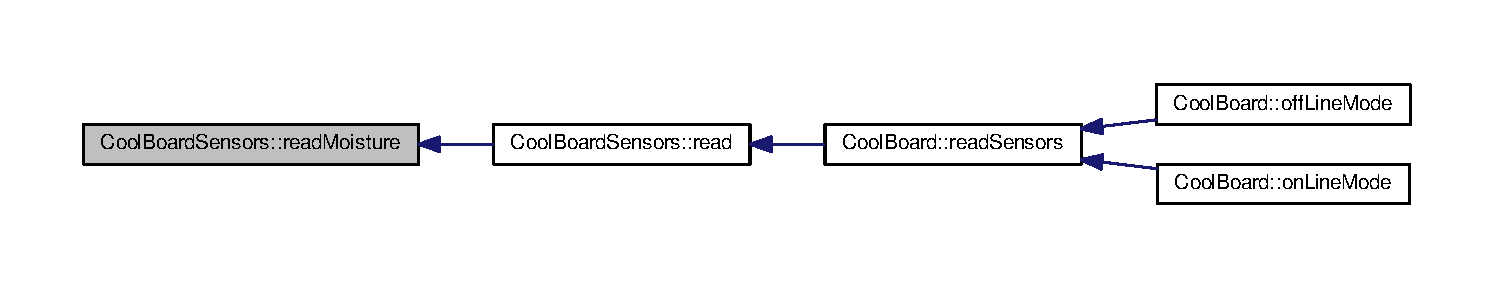
\includegraphics[width=350pt]{classCoolBoardSensors_a8761bff50373c485f4465c8db47d0633_icgraph}
\end{center}
\end{figure}
\mbox{\Hypertarget{classCoolBoardSensors_a6944b6ea7bce8e2fce1b434acfd9d5f3}\label{classCoolBoardSensors_a6944b6ea7bce8e2fce1b434acfd9d5f3}} 
\index{Cool\+Board\+Sensors@{Cool\+Board\+Sensors}!read\+V\+Bat@{read\+V\+Bat}}
\index{read\+V\+Bat@{read\+V\+Bat}!Cool\+Board\+Sensors@{Cool\+Board\+Sensors}}
\subsubsection{\texorpdfstring{read\+V\+Bat()}{readVBat()}}
{\footnotesize\ttfamily float Cool\+Board\+Sensors\+::read\+V\+Bat (\begin{DoxyParamCaption}{ }\end{DoxyParamCaption})}

\hyperlink{classCoolBoardSensors_a6944b6ea7bce8e2fce1b434acfd9d5f3}{Cool\+Board\+Sensors\+::read\+V\+Bat()}\+: This method is provided to read the Battery Voltage.

\begin{DoxyReturn}{Returns}
a float representing the battery voltage 
\end{DoxyReturn}


Definition at line 423 of file Cool\+Board\+Sensors.\+cpp.



References An\+Mplex.



Referenced by read().


\begin{DoxyCode}
424 \{
425     digitalWrite(\hyperlink{classCoolBoardSensors_a12ef28b1046219e0aee10bf64e28c4a5}{AnMplex}, LOW);                                  \textcolor{comment}{//Enable Analog Switch to get the
       batterie tension}
426     
427     delay(200);
428     
429     \textcolor{keywordtype}{int} raw = analogRead(A0);                                    \textcolor{comment}{//read in batterie tension}
430     
431     \textcolor{keywordtype}{float} val = 6.04 / 1024 * raw;                               \textcolor{comment}{//convert it apprimatly right tension in
       volts}
432 
433     \textcolor{keywordflow}{return} (val);   
434 \}
\end{DoxyCode}
Here is the caller graph for this function\+:
\nopagebreak
\begin{figure}[H]
\begin{center}
\leavevmode
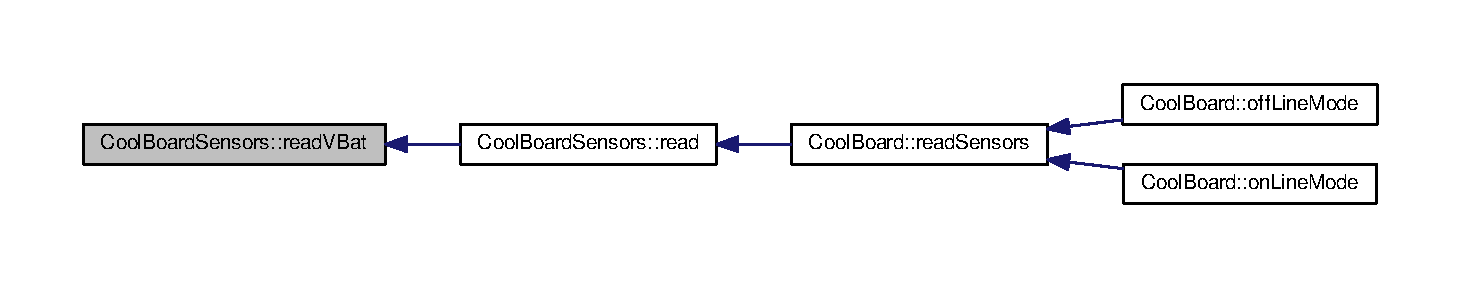
\includegraphics[width=350pt]{classCoolBoardSensors_a6944b6ea7bce8e2fce1b434acfd9d5f3_icgraph}
\end{center}
\end{figure}
\mbox{\Hypertarget{classCoolBoardSensors_a406307ffd70272282d91479c7ed8d66f}\label{classCoolBoardSensors_a406307ffd70272282d91479c7ed8d66f}} 
\index{Cool\+Board\+Sensors@{Cool\+Board\+Sensors}!set\+Env\+Sensor\+Settings@{set\+Env\+Sensor\+Settings}}
\index{set\+Env\+Sensor\+Settings@{set\+Env\+Sensor\+Settings}!Cool\+Board\+Sensors@{Cool\+Board\+Sensors}}
\subsubsection{\texorpdfstring{set\+Env\+Sensor\+Settings()}{setEnvSensorSettings()}}
{\footnotesize\ttfamily void Cool\+Board\+Sensors\+::set\+Env\+Sensor\+Settings (\begin{DoxyParamCaption}\item[{uint8\+\_\+t}]{comm\+Interface = {\ttfamily I2C\+\_\+MODE},  }\item[{uint8\+\_\+t}]{I2\+C\+Address = {\ttfamily 0x76},  }\item[{uint8\+\_\+t}]{run\+Mode = {\ttfamily 3},  }\item[{uint8\+\_\+t}]{t\+Standby = {\ttfamily 0},  }\item[{uint8\+\_\+t}]{filter = {\ttfamily 0},  }\item[{uint8\+\_\+t}]{temp\+Over\+Sample = {\ttfamily 1},  }\item[{uint8\+\_\+t}]{press\+Over\+Sample = {\ttfamily 1},  }\item[{uint8\+\_\+t}]{humid\+Over\+Sample = {\ttfamily 1} }\end{DoxyParamCaption})}

Cool\+Board\+Sensors\+::set\+Env\+Sensor\+Setting()\+: This method is provided to set the enviornment sensor settings , if argument is ommitted , default value will be assigned 

Definition at line 391 of file Cool\+Board\+Sensors.\+cpp.



References env\+Sensor.



Referenced by begin().


\begin{DoxyCode}
396 \{
397   \hyperlink{classCoolBoardSensors_a868e38985e9a2412829fa2790ca13e2e}{envSensor}.settings.commInterface = commInterface;      
398   
399   \hyperlink{classCoolBoardSensors_a868e38985e9a2412829fa2790ca13e2e}{envSensor}.settings.I2CAddress = I2CAddress;
400   
401   \hyperlink{classCoolBoardSensors_a868e38985e9a2412829fa2790ca13e2e}{envSensor}.settings.runMode = runMode; 
402   
403   \hyperlink{classCoolBoardSensors_a868e38985e9a2412829fa2790ca13e2e}{envSensor}.settings.tStandby = tStandby; 
404   
405   \hyperlink{classCoolBoardSensors_a868e38985e9a2412829fa2790ca13e2e}{envSensor}.settings.filter = filter; 
406   
407   \hyperlink{classCoolBoardSensors_a868e38985e9a2412829fa2790ca13e2e}{envSensor}.settings.tempOverSample = tempOverSample;
408   
409   \hyperlink{classCoolBoardSensors_a868e38985e9a2412829fa2790ca13e2e}{envSensor}.settings.pressOverSample = pressOverSample;
410   
411   \hyperlink{classCoolBoardSensors_a868e38985e9a2412829fa2790ca13e2e}{envSensor}.settings.humidOverSample = humidOverSample;
412 
413 \}
\end{DoxyCode}
Here is the caller graph for this function\+:
\nopagebreak
\begin{figure}[H]
\begin{center}
\leavevmode
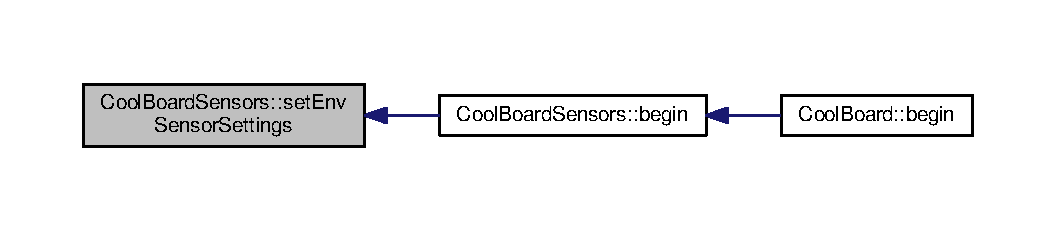
\includegraphics[width=350pt]{classCoolBoardSensors_a406307ffd70272282d91479c7ed8d66f_icgraph}
\end{center}
\end{figure}
\mbox{\Hypertarget{classCoolBoardSensors_ab76e6dbd6efbcc25ff460535badd8d45}\label{classCoolBoardSensors_ab76e6dbd6efbcc25ff460535badd8d45}} 
\index{Cool\+Board\+Sensors@{Cool\+Board\+Sensors}!set\+Json\+Size@{set\+Json\+Size}}
\index{set\+Json\+Size@{set\+Json\+Size}!Cool\+Board\+Sensors@{Cool\+Board\+Sensors}}
\subsubsection{\texorpdfstring{set\+Json\+Size()}{setJsonSize()}}
{\footnotesize\ttfamily void Cool\+Board\+Sensors\+::set\+Json\+Size (\begin{DoxyParamCaption}\item[{int}]{json\+Size }\end{DoxyParamCaption})}

Cool\+Board\+Sensors\+::set\+Json\+Size( J\+S\+O\+N size)\+: This method is provided to set the sensor board answer size 

Definition at line 51 of file Cool\+Board\+Sensors.\+cpp.



References json\+Size.


\begin{DoxyCode}
52 \{
53     this->\hyperlink{classCoolBoardSensors_a05a40dc80bfff14ffb830f549b876f8d}{jsonSize}=\hyperlink{classCoolBoardSensors_a05a40dc80bfff14ffb830f549b876f8d}{jsonSize};
54 \}
\end{DoxyCode}
\mbox{\Hypertarget{classCoolBoardSensors_ab67b900b9e5e7c18d52d2d9107ba171b}\label{classCoolBoardSensors_ab67b900b9e5e7c18d52d2d9107ba171b}} 
\index{Cool\+Board\+Sensors@{Cool\+Board\+Sensors}!stop\+Read\+I2C@{stop\+Read\+I2C}}
\index{stop\+Read\+I2C@{stop\+Read\+I2C}!Cool\+Board\+Sensors@{Cool\+Board\+Sensors}}
\subsubsection{\texorpdfstring{stop\+Read\+I2\+C()}{stopReadI2C()}}
{\footnotesize\ttfamily void Cool\+Board\+Sensors\+::stop\+Read\+I2C (\begin{DoxyParamCaption}{ }\end{DoxyParamCaption})}

\hyperlink{classCoolBoardSensors_ab67b900b9e5e7c18d52d2d9107ba171b}{Cool\+Board\+Sensors\+::stop\+Read\+I2\+C()}\+: This method is provided to disable the I2C Interface on the sensor board 

Definition at line 205 of file Cool\+Board\+Sensors.\+cpp.



References En\+I2C.


\begin{DoxyCode}
206 \{
207 
208     digitalWrite(\hyperlink{classCoolBoardSensors_aaa6b5dbf3a6633bffd9d204d961096dc}{EnI2C},LOW);\textcolor{comment}{//HIGH= I2C Enable}
209 
210 \}
\end{DoxyCode}


\subsection{Member Data Documentation}
\mbox{\Hypertarget{classCoolBoardSensors_abff8dfeccb2f7689847bb64d5f1cd31e}\label{classCoolBoardSensors_abff8dfeccb2f7689847bb64d5f1cd31e}} 
\index{Cool\+Board\+Sensors@{Cool\+Board\+Sensors}!air\+Data\+Active@{air\+Data\+Active}}
\index{air\+Data\+Active@{air\+Data\+Active}!Cool\+Board\+Sensors@{Cool\+Board\+Sensors}}
\subsubsection{\texorpdfstring{air\+Data\+Active}{airDataActive}}
{\footnotesize\ttfamily struct \hyperlink{structCoolBoardSensors_1_1airActive}{Cool\+Board\+Sensors\+::air\+Active} Cool\+Board\+Sensors\+::air\+Data\+Active\hspace{0.3cm}{\ttfamily [private]}}



Referenced by all\+Active(), config(), print\+Conf(), and read().

\mbox{\Hypertarget{classCoolBoardSensors_a12ef28b1046219e0aee10bf64e28c4a5}\label{classCoolBoardSensors_a12ef28b1046219e0aee10bf64e28c4a5}} 
\index{Cool\+Board\+Sensors@{Cool\+Board\+Sensors}!An\+Mplex@{An\+Mplex}}
\index{An\+Mplex@{An\+Mplex}!Cool\+Board\+Sensors@{Cool\+Board\+Sensors}}
\subsubsection{\texorpdfstring{An\+Mplex}{AnMplex}}
{\footnotesize\ttfamily const int Cool\+Board\+Sensors\+::\+An\+Mplex = 12\hspace{0.3cm}{\ttfamily [private]}}



Definition at line 101 of file Cool\+Board\+Sensors.\+h.



Referenced by Cool\+Board\+Sensors(), read\+Moisture(), and read\+V\+Bat().

\mbox{\Hypertarget{classCoolBoardSensors_a46dfddb8a12720e92cd2825ef09023c8}\label{classCoolBoardSensors_a46dfddb8a12720e92cd2825ef09023c8}} 
\index{Cool\+Board\+Sensors@{Cool\+Board\+Sensors}!earth\+Moisture\+Active@{earth\+Moisture\+Active}}
\index{earth\+Moisture\+Active@{earth\+Moisture\+Active}!Cool\+Board\+Sensors@{Cool\+Board\+Sensors}}
\subsubsection{\texorpdfstring{earth\+Moisture\+Active}{earthMoistureActive}}
{\footnotesize\ttfamily byte Cool\+Board\+Sensors\+::earth\+Moisture\+Active\hspace{0.3cm}{\ttfamily [private]}}



Definition at line 105 of file Cool\+Board\+Sensors.\+h.



Referenced by all\+Active(), config(), print\+Conf(), and read().

\mbox{\Hypertarget{classCoolBoardSensors_aaa6b5dbf3a6633bffd9d204d961096dc}\label{classCoolBoardSensors_aaa6b5dbf3a6633bffd9d204d961096dc}} 
\index{Cool\+Board\+Sensors@{Cool\+Board\+Sensors}!En\+I2C@{En\+I2C}}
\index{En\+I2C@{En\+I2C}!Cool\+Board\+Sensors@{Cool\+Board\+Sensors}}
\subsubsection{\texorpdfstring{En\+I2C}{EnI2C}}
{\footnotesize\ttfamily const int Cool\+Board\+Sensors\+::\+En\+I2C = 5\hspace{0.3cm}{\ttfamily [private]}}



Definition at line 102 of file Cool\+Board\+Sensors.\+h.



Referenced by Cool\+Board\+Sensors(), init\+Read\+I2\+C(), and stop\+Read\+I2\+C().

\mbox{\Hypertarget{classCoolBoardSensors_a6177d02e14a057a2f171a2e930b5038d}\label{classCoolBoardSensors_a6177d02e14a057a2f171a2e930b5038d}} 
\index{Cool\+Board\+Sensors@{Cool\+Board\+Sensors}!En\+Moisture@{En\+Moisture}}
\index{En\+Moisture@{En\+Moisture}!Cool\+Board\+Sensors@{Cool\+Board\+Sensors}}
\subsubsection{\texorpdfstring{En\+Moisture}{EnMoisture}}
{\footnotesize\ttfamily const int Cool\+Board\+Sensors\+::\+En\+Moisture = 13\hspace{0.3cm}{\ttfamily [private]}}



Definition at line 100 of file Cool\+Board\+Sensors.\+h.



Referenced by Cool\+Board\+Sensors(), and read\+Moisture().

\mbox{\Hypertarget{classCoolBoardSensors_a868e38985e9a2412829fa2790ca13e2e}\label{classCoolBoardSensors_a868e38985e9a2412829fa2790ca13e2e}} 
\index{Cool\+Board\+Sensors@{Cool\+Board\+Sensors}!env\+Sensor@{env\+Sensor}}
\index{env\+Sensor@{env\+Sensor}!Cool\+Board\+Sensors@{Cool\+Board\+Sensors}}
\subsubsection{\texorpdfstring{env\+Sensor}{envSensor}}
{\footnotesize\ttfamily B\+M\+E280 Cool\+Board\+Sensors\+::env\+Sensor}



Definition at line 77 of file Cool\+Board\+Sensors.\+h.



Referenced by begin(), read(), and set\+Env\+Sensor\+Settings().

\mbox{\Hypertarget{classCoolBoardSensors_a05a40dc80bfff14ffb830f549b876f8d}\label{classCoolBoardSensors_a05a40dc80bfff14ffb830f549b876f8d}} 
\index{Cool\+Board\+Sensors@{Cool\+Board\+Sensors}!json\+Size@{json\+Size}}
\index{json\+Size@{json\+Size}!Cool\+Board\+Sensors@{Cool\+Board\+Sensors}}
\subsubsection{\texorpdfstring{json\+Size}{jsonSize}}
{\footnotesize\ttfamily int Cool\+Board\+Sensors\+::json\+Size\hspace{0.3cm}{\ttfamily [private]}}



Definition at line 107 of file Cool\+Board\+Sensors.\+h.



Referenced by config(), get\+Json\+Size(), print\+Conf(), read(), and set\+Json\+Size().

\mbox{\Hypertarget{classCoolBoardSensors_ac4deb1cf41bac8b91c780c92fab00ba4}\label{classCoolBoardSensors_ac4deb1cf41bac8b91c780c92fab00ba4}} 
\index{Cool\+Board\+Sensors@{Cool\+Board\+Sensors}!light\+Data\+Active@{light\+Data\+Active}}
\index{light\+Data\+Active@{light\+Data\+Active}!Cool\+Board\+Sensors@{Cool\+Board\+Sensors}}
\subsubsection{\texorpdfstring{light\+Data\+Active}{lightDataActive}}
{\footnotesize\ttfamily struct \hyperlink{structCoolBoardSensors_1_1lightActive}{Cool\+Board\+Sensors\+::light\+Active} Cool\+Board\+Sensors\+::light\+Data\+Active\hspace{0.3cm}{\ttfamily [private]}}



Referenced by all\+Active(), config(), print\+Conf(), and read().

\mbox{\Hypertarget{classCoolBoardSensors_a3e397300fb707dd193e909a757bf6102}\label{classCoolBoardSensors_a3e397300fb707dd193e909a757bf6102}} 
\index{Cool\+Board\+Sensors@{Cool\+Board\+Sensors}!light\+Sensor@{light\+Sensor}}
\index{light\+Sensor@{light\+Sensor}!Cool\+Board\+Sensors@{Cool\+Board\+Sensors}}
\subsubsection{\texorpdfstring{light\+Sensor}{lightSensor}}
{\footnotesize\ttfamily S\+I114X Cool\+Board\+Sensors\+::light\+Sensor = S\+I114X()}



Definition at line 75 of file Cool\+Board\+Sensors.\+h.



Referenced by begin(), end(), and read().

\mbox{\Hypertarget{classCoolBoardSensors_af5039ad760b0ff0aa7eee16c55e81702}\label{classCoolBoardSensors_af5039ad760b0ff0aa7eee16c55e81702}} 
\index{Cool\+Board\+Sensors@{Cool\+Board\+Sensors}!vbat\+Active@{vbat\+Active}}
\index{vbat\+Active@{vbat\+Active}!Cool\+Board\+Sensors@{Cool\+Board\+Sensors}}
\subsubsection{\texorpdfstring{vbat\+Active}{vbatActive}}
{\footnotesize\ttfamily byte Cool\+Board\+Sensors\+::vbat\+Active\hspace{0.3cm}{\ttfamily [private]}}



Definition at line 104 of file Cool\+Board\+Sensors.\+h.



Referenced by all\+Active(), config(), print\+Conf(), and read().



The documentation for this class was generated from the following files\+:\begin{DoxyCompactItemize}
\item 
\hyperlink{CoolBoardSensors_8h}{Cool\+Board\+Sensors.\+h}\item 
\hyperlink{CoolBoardSensors_8cpp}{Cool\+Board\+Sensors.\+cpp}\end{DoxyCompactItemize}

\hypertarget{structCoolBoardSensors_1_1airActive}{}\section{Cool\+Board\+Sensors\+:\+:air\+Active Struct Reference}
\label{structCoolBoardSensors_1_1airActive}\index{Cool\+Board\+Sensors\+::air\+Active@{Cool\+Board\+Sensors\+::air\+Active}}


Collaboration diagram for Cool\+Board\+Sensors\+:\+:air\+Active\+:\nopagebreak
\begin{figure}[H]
\begin{center}
\leavevmode
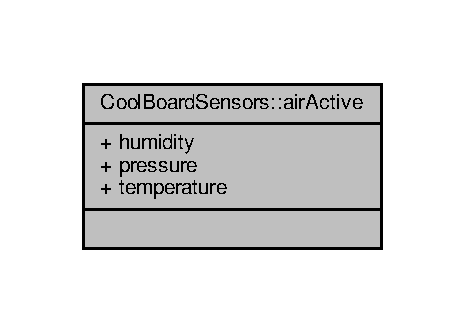
\includegraphics[width=223pt]{structCoolBoardSensors_1_1airActive__coll__graph}
\end{center}
\end{figure}
\subsection*{Public Attributes}
\begin{DoxyCompactItemize}
\item 
byte \hyperlink{structCoolBoardSensors_1_1airActive_a9a6633c426b0508e30ebc1832ec6d745}{temperature} =0
\item 
byte \hyperlink{structCoolBoardSensors_1_1airActive_ae5740445054b27415e22f450576accb7}{humidity} =0
\item 
byte \hyperlink{structCoolBoardSensors_1_1airActive_ab200826a70d1dc9945f5efb6b9c732ed}{pressure} =0
\end{DoxyCompactItemize}


\subsection{Detailed Description}


Definition at line 77 of file Cool\+Board\+Sensors.\+h.



\subsection{Member Data Documentation}
\mbox{\Hypertarget{structCoolBoardSensors_1_1airActive_ae5740445054b27415e22f450576accb7}\label{structCoolBoardSensors_1_1airActive_ae5740445054b27415e22f450576accb7}} 
\index{Cool\+Board\+Sensors\+::air\+Active@{Cool\+Board\+Sensors\+::air\+Active}!humidity@{humidity}}
\index{humidity@{humidity}!Cool\+Board\+Sensors\+::air\+Active@{Cool\+Board\+Sensors\+::air\+Active}}
\subsubsection{\texorpdfstring{humidity}{humidity}}
{\footnotesize\ttfamily byte Cool\+Board\+Sensors\+::air\+Active\+::humidity =0}



Definition at line 80 of file Cool\+Board\+Sensors.\+h.



Referenced by Cool\+Board\+Sensors\+::all\+Active(), Cool\+Board\+Sensors\+::config(), Cool\+Board\+Sensors\+::print\+Conf(), and Cool\+Board\+Sensors\+::read().

\mbox{\Hypertarget{structCoolBoardSensors_1_1airActive_ab200826a70d1dc9945f5efb6b9c732ed}\label{structCoolBoardSensors_1_1airActive_ab200826a70d1dc9945f5efb6b9c732ed}} 
\index{Cool\+Board\+Sensors\+::air\+Active@{Cool\+Board\+Sensors\+::air\+Active}!pressure@{pressure}}
\index{pressure@{pressure}!Cool\+Board\+Sensors\+::air\+Active@{Cool\+Board\+Sensors\+::air\+Active}}
\subsubsection{\texorpdfstring{pressure}{pressure}}
{\footnotesize\ttfamily byte Cool\+Board\+Sensors\+::air\+Active\+::pressure =0}



Definition at line 81 of file Cool\+Board\+Sensors.\+h.



Referenced by Cool\+Board\+Sensors\+::all\+Active(), Cool\+Board\+Sensors\+::config(), Cool\+Board\+Sensors\+::print\+Conf(), and Cool\+Board\+Sensors\+::read().

\mbox{\Hypertarget{structCoolBoardSensors_1_1airActive_a9a6633c426b0508e30ebc1832ec6d745}\label{structCoolBoardSensors_1_1airActive_a9a6633c426b0508e30ebc1832ec6d745}} 
\index{Cool\+Board\+Sensors\+::air\+Active@{Cool\+Board\+Sensors\+::air\+Active}!temperature@{temperature}}
\index{temperature@{temperature}!Cool\+Board\+Sensors\+::air\+Active@{Cool\+Board\+Sensors\+::air\+Active}}
\subsubsection{\texorpdfstring{temperature}{temperature}}
{\footnotesize\ttfamily byte Cool\+Board\+Sensors\+::air\+Active\+::temperature =0}



Definition at line 79 of file Cool\+Board\+Sensors.\+h.



Referenced by Cool\+Board\+Sensors\+::all\+Active(), Cool\+Board\+Sensors\+::config(), Cool\+Board\+Sensors\+::print\+Conf(), and Cool\+Board\+Sensors\+::read().



The documentation for this struct was generated from the following file\+:\begin{DoxyCompactItemize}
\item 
/home/ashiroji/\+Arduino/libraries/\+Cool\+Board/\hyperlink{CoolBoardSensors_8h}{Cool\+Board\+Sensors.\+h}\end{DoxyCompactItemize}

\hypertarget{structCoolBoardSensors_1_1lightActive}{}\section{Cool\+Board\+Sensors\+:\+:light\+Active Struct Reference}
\label{structCoolBoardSensors_1_1lightActive}\index{Cool\+Board\+Sensors\+::light\+Active@{Cool\+Board\+Sensors\+::light\+Active}}


Collaboration diagram for Cool\+Board\+Sensors\+:\+:light\+Active\+:\nopagebreak
\begin{figure}[H]
\begin{center}
\leavevmode
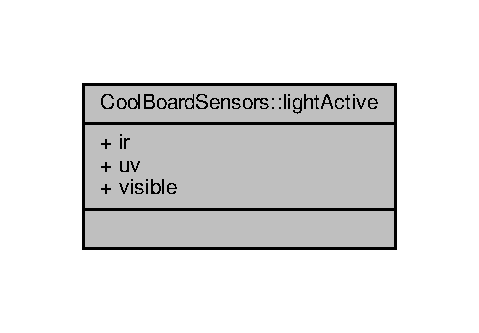
\includegraphics[width=230pt]{structCoolBoardSensors_1_1lightActive__coll__graph}
\end{center}
\end{figure}
\subsection*{Public Attributes}
\begin{DoxyCompactItemize}
\item 
byte \hyperlink{structCoolBoardSensors_1_1lightActive_abcbba296b6a95e67c0cd2555d9dd50c7}{visible} =0
\item 
byte \hyperlink{structCoolBoardSensors_1_1lightActive_a67700895349b95ceb263f1a6da756315}{ir} =0
\item 
byte \hyperlink{structCoolBoardSensors_1_1lightActive_a949a7aaf5166d981de8fe0fd93da20d6}{uv} =0
\end{DoxyCompactItemize}


\subsection{Detailed Description}


Definition at line 81 of file Cool\+Board\+Sensors.\+h.



\subsection{Member Data Documentation}
\mbox{\Hypertarget{structCoolBoardSensors_1_1lightActive_a67700895349b95ceb263f1a6da756315}\label{structCoolBoardSensors_1_1lightActive_a67700895349b95ceb263f1a6da756315}} 
\index{Cool\+Board\+Sensors\+::light\+Active@{Cool\+Board\+Sensors\+::light\+Active}!ir@{ir}}
\index{ir@{ir}!Cool\+Board\+Sensors\+::light\+Active@{Cool\+Board\+Sensors\+::light\+Active}}
\subsubsection{\texorpdfstring{ir}{ir}}
{\footnotesize\ttfamily byte Cool\+Board\+Sensors\+::light\+Active\+::ir =0}



Definition at line 84 of file Cool\+Board\+Sensors.\+h.



Referenced by Cool\+Board\+Sensors\+::all\+Active(), Cool\+Board\+Sensors\+::config(), Cool\+Board\+Sensors\+::print\+Conf(), and Cool\+Board\+Sensors\+::read().

\mbox{\Hypertarget{structCoolBoardSensors_1_1lightActive_a949a7aaf5166d981de8fe0fd93da20d6}\label{structCoolBoardSensors_1_1lightActive_a949a7aaf5166d981de8fe0fd93da20d6}} 
\index{Cool\+Board\+Sensors\+::light\+Active@{Cool\+Board\+Sensors\+::light\+Active}!uv@{uv}}
\index{uv@{uv}!Cool\+Board\+Sensors\+::light\+Active@{Cool\+Board\+Sensors\+::light\+Active}}
\subsubsection{\texorpdfstring{uv}{uv}}
{\footnotesize\ttfamily byte Cool\+Board\+Sensors\+::light\+Active\+::uv =0}



Definition at line 85 of file Cool\+Board\+Sensors.\+h.



Referenced by Cool\+Board\+Sensors\+::all\+Active(), Cool\+Board\+Sensors\+::config(), Cool\+Board\+Sensors\+::print\+Conf(), and Cool\+Board\+Sensors\+::read().

\mbox{\Hypertarget{structCoolBoardSensors_1_1lightActive_abcbba296b6a95e67c0cd2555d9dd50c7}\label{structCoolBoardSensors_1_1lightActive_abcbba296b6a95e67c0cd2555d9dd50c7}} 
\index{Cool\+Board\+Sensors\+::light\+Active@{Cool\+Board\+Sensors\+::light\+Active}!visible@{visible}}
\index{visible@{visible}!Cool\+Board\+Sensors\+::light\+Active@{Cool\+Board\+Sensors\+::light\+Active}}
\subsubsection{\texorpdfstring{visible}{visible}}
{\footnotesize\ttfamily byte Cool\+Board\+Sensors\+::light\+Active\+::visible =0}



Definition at line 83 of file Cool\+Board\+Sensors.\+h.



Referenced by Cool\+Board\+Sensors\+::all\+Active(), Cool\+Board\+Sensors\+::config(), Cool\+Board\+Sensors\+::print\+Conf(), and Cool\+Board\+Sensors\+::read().



The documentation for this struct was generated from the following file\+:\begin{DoxyCompactItemize}
\item 
/home/ashiroji/\+Arduino/libraries/\+Cool\+Board/\hyperlink{CoolBoardSensors_8h}{Cool\+Board\+Sensors.\+h}\end{DoxyCompactItemize}

\hypertarget{classCoolFileSystem}{}\section{Cool\+File\+System Class Reference}
\label{classCoolFileSystem}\index{Cool\+File\+System@{Cool\+File\+System}}


This class handles the file system.  




{\ttfamily \#include $<$Cool\+File\+System.\+h$>$}



Collaboration diagram for Cool\+File\+System\+:\nopagebreak
\begin{figure}[H]
\begin{center}
\leavevmode
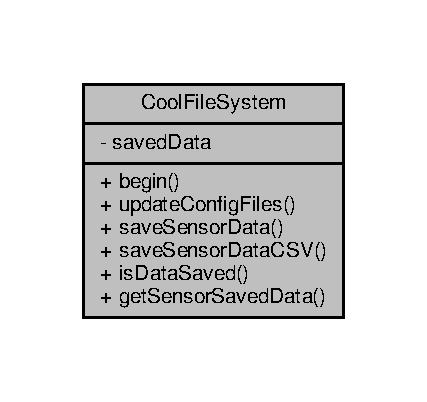
\includegraphics[width=205pt]{classCoolFileSystem__coll__graph}
\end{center}
\end{figure}
\subsection*{Public Member Functions}
\begin{DoxyCompactItemize}
\item 
bool \hyperlink{classCoolFileSystem_a6ba6f666ed4c530174f8569d2c636748}{begin} ()
\item 
bool \hyperlink{classCoolFileSystem_a32dad79ae80182a83e2e8f52286b7c7b}{update\+Config\+Files} (String answer, int J\+S\+O\+N\+\_\+\+S\+I\+ZE)
\item 
bool \hyperlink{classCoolFileSystem_a4c560c2ddd40b74b7758e6ceb2c58957}{save\+Sensor\+Data} (const char $\ast$data, int Sensor\+\_\+\+J\+S\+O\+N\+\_\+\+S\+I\+ZE)
\item 
bool \hyperlink{classCoolFileSystem_a5a7eaeea7a9fbf8aaef651d862fa3b5b}{is\+Data\+Saved} ()
\item 
String \hyperlink{classCoolFileSystem_a5c58bca3735c0ed3efb268d70ef998ef}{get\+Sensor\+Saved\+Data} ()
\end{DoxyCompactItemize}
\subsection*{Private Attributes}
\begin{DoxyCompactItemize}
\item 
bool \hyperlink{classCoolFileSystem_ad398e0c5c41a0c88acdf5d672aa71351}{saved\+Data} =0
\end{DoxyCompactItemize}


\subsection{Detailed Description}
This class handles the file system. 

Definition at line 22 of file Cool\+File\+System.\+h.



\subsection{Member Function Documentation}
\mbox{\Hypertarget{classCoolFileSystem_a6ba6f666ed4c530174f8569d2c636748}\label{classCoolFileSystem_a6ba6f666ed4c530174f8569d2c636748}} 
\index{Cool\+File\+System@{Cool\+File\+System}!begin@{begin}}
\index{begin@{begin}!Cool\+File\+System@{Cool\+File\+System}}
\subsubsection{\texorpdfstring{begin()}{begin()}}
{\footnotesize\ttfamily bool Cool\+File\+System\+::begin (\begin{DoxyParamCaption}{ }\end{DoxyParamCaption})}

\hyperlink{classCoolFileSystem_a6ba6f666ed4c530174f8569d2c636748}{Cool\+File\+System\+::begin()}\+: This method is provided to start the S\+P\+I\+F\+FS object.

\begin{DoxyReturn}{Returns}
true if S\+P\+I\+F\+FS was initialized correctly, false otherwise 
\end{DoxyReturn}


Definition at line 22 of file Cool\+File\+System.\+cpp.



Referenced by Cool\+Board\+::begin(), and Cool\+Board\+::config().


\begin{DoxyCode}
23 \{
24     Serial.println(\textcolor{stringliteral}{"Entering CoolFileSystem.begin()"});
25     Serial.println();
26     
27     Serial.print(\textcolor{stringliteral}{"SPIFFS success ? "});
28     Serial.println(SPIFFS.begin());
29     Serial.println();
30     
31     \textcolor{keywordflow}{return}( SPIFFS.begin() );                                   \textcolor{comment}{//Initialize Filesystem}
32 
33 \}
\end{DoxyCode}
Here is the caller graph for this function\+:\nopagebreak
\begin{figure}[H]
\begin{center}
\leavevmode
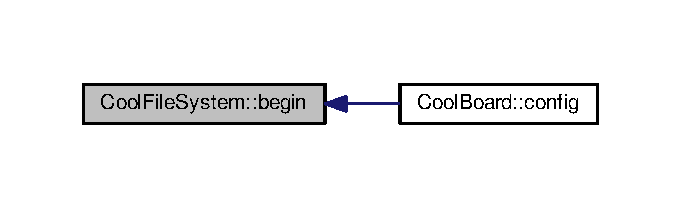
\includegraphics[width=350pt]{classCoolFileSystem_a6ba6f666ed4c530174f8569d2c636748_icgraph}
\end{center}
\end{figure}
\mbox{\Hypertarget{classCoolFileSystem_a5c58bca3735c0ed3efb268d70ef998ef}\label{classCoolFileSystem_a5c58bca3735c0ed3efb268d70ef998ef}} 
\index{Cool\+File\+System@{Cool\+File\+System}!get\+Sensor\+Saved\+Data@{get\+Sensor\+Saved\+Data}}
\index{get\+Sensor\+Saved\+Data@{get\+Sensor\+Saved\+Data}!Cool\+File\+System@{Cool\+File\+System}}
\subsubsection{\texorpdfstring{get\+Sensor\+Saved\+Data()}{getSensorSavedData()}}
{\footnotesize\ttfamily String Cool\+File\+System\+::get\+Sensor\+Saved\+Data (\begin{DoxyParamCaption}{ }\end{DoxyParamCaption})}

Cool\+File\+System\+::get\+Sensor\+Data()\+: This method is provided to return the sensor data saved in the File System

\begin{DoxyReturn}{Returns}
string json of the saved sensor data file 
\end{DoxyReturn}


Definition at line 356 of file Cool\+File\+System.\+cpp.



References saved\+Data.



Referenced by Cool\+Board\+::on\+Line\+Mode().


\begin{DoxyCode}
357 \{
358     Serial.println(\textcolor{stringliteral}{"Entering CoolFileSystem.getSensorSavedData()"});
359     Serial.println();
360 
361     \textcolor{comment}{//open sensors data file}
362     File sensorsData=SPIFFS.open(\textcolor{stringliteral}{"/sensorsData.json"},\textcolor{stringliteral}{"r"});
363     
364     \textcolor{keywordflow}{if} (!sensorsData)
365     \{
366         Serial.println(\textcolor{stringliteral}{"Failed to read /sensorsData.json"}); 
367         \textcolor{keywordflow}{return}(\textcolor{stringliteral}{"failed to open file"});
368     \}
369     \textcolor{keywordflow}{else}
370     \{
371         \textcolor{keywordtype}{size\_t} size = sensorsData.size();
372 
373         \textcolor{comment}{// Allocate a buffer to store contents of the file.}
374         std::unique\_ptr < char[] > buf(\textcolor{keyword}{new} \textcolor{keywordtype}{char}[size]);
375 
376         sensorsData.readBytes(buf.get(), size);
377 
378         DynamicJsonBuffer jsonBuffer;
379 
380         JsonObject & json = jsonBuffer.parseObject(buf.get());
381         
382         \textcolor{keywordflow}{if} (!json.success())
383         \{
384             \textcolor{keywordflow}{return}(\textcolor{stringliteral}{"failed to parse json"});
385         \}
386         \textcolor{keywordflow}{else}
387         \{   
388             \textcolor{comment}{//the return string}
389             String sensorDataString;
390             
391             \textcolor{comment}{//print the json to the string}
392             json.printTo(sensorDataString);
393             
394             \textcolor{comment}{//close the file}
395             sensorsData.close();
396 
397             \textcolor{comment}{//delete data in the file}
398             File sensorsData=SPIFFS.open(\textcolor{stringliteral}{"/sensorsData.json"},\textcolor{stringliteral}{"w"});
399             \textcolor{keywordflow}{if} (!sensorsData)   
400             \{
401                 \textcolor{keywordflow}{return}(\textcolor{stringliteral}{"failed to delete data in the file"});
402             \}
403 
404             sensorsData.close();
405             
406             \textcolor{comment}{//position the saved data flag to false}
407             this->\hyperlink{classCoolFileSystem_ad398e0c5c41a0c88acdf5d672aa71351}{savedData}=\textcolor{keyword}{false}; 
408         
409             Serial.println(\textcolor{stringliteral}{"saved data : "});
410             Serial.println(sensorDataString);
411             Serial.println();
412 
413             \textcolor{comment}{//return the string}
414             \textcolor{keywordflow}{return}(sensorDataString);       
415         \}
416         
417         
418     \}
419 
420 \}
\end{DoxyCode}
Here is the caller graph for this function\+:\nopagebreak
\begin{figure}[H]
\begin{center}
\leavevmode
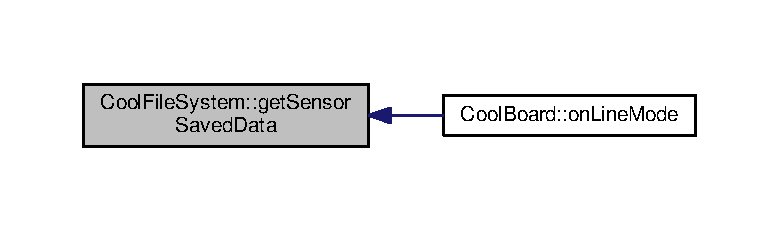
\includegraphics[width=350pt]{classCoolFileSystem_a5c58bca3735c0ed3efb268d70ef998ef_icgraph}
\end{center}
\end{figure}
\mbox{\Hypertarget{classCoolFileSystem_a5a7eaeea7a9fbf8aaef651d862fa3b5b}\label{classCoolFileSystem_a5a7eaeea7a9fbf8aaef651d862fa3b5b}} 
\index{Cool\+File\+System@{Cool\+File\+System}!is\+Data\+Saved@{is\+Data\+Saved}}
\index{is\+Data\+Saved@{is\+Data\+Saved}!Cool\+File\+System@{Cool\+File\+System}}
\subsubsection{\texorpdfstring{is\+Data\+Saved()}{isDataSaved()}}
{\footnotesize\ttfamily bool Cool\+File\+System\+::is\+Data\+Saved (\begin{DoxyParamCaption}{ }\end{DoxyParamCaption})}

\hyperlink{classCoolFileSystem_a5a7eaeea7a9fbf8aaef651d862fa3b5b}{Cool\+File\+System\+::is\+Data\+Saved()}\+: This method is provided to report wether there is sensor data saved in the File System.

\begin{DoxyReturn}{Returns}
true if there is data saved, false otherwise 
\end{DoxyReturn}


Definition at line 337 of file Cool\+File\+System.\+cpp.



References saved\+Data.



Referenced by Cool\+Board\+::on\+Line\+Mode().


\begin{DoxyCode}
338 \{
339     Serial.println(\textcolor{stringliteral}{"Entering CoolFileSystem.isDataSaved()"});
340     Serial.println();
341     
342     Serial.print(\textcolor{stringliteral}{"savedData : "});
343     Serial.println(this->\hyperlink{classCoolFileSystem_ad398e0c5c41a0c88acdf5d672aa71351}{savedData});
344 
345     \textcolor{keywordflow}{return}( this->\hyperlink{classCoolFileSystem_ad398e0c5c41a0c88acdf5d672aa71351}{savedData} );
346 \}
\end{DoxyCode}
Here is the caller graph for this function\+:\nopagebreak
\begin{figure}[H]
\begin{center}
\leavevmode
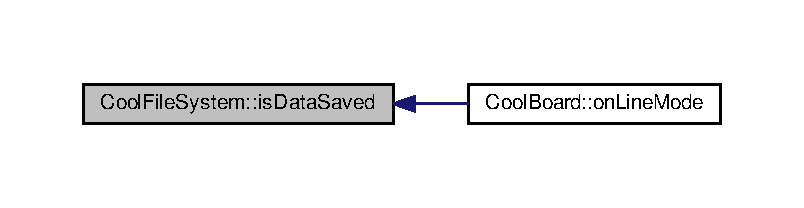
\includegraphics[width=350pt]{classCoolFileSystem_a5a7eaeea7a9fbf8aaef651d862fa3b5b_icgraph}
\end{center}
\end{figure}
\mbox{\Hypertarget{classCoolFileSystem_a4c560c2ddd40b74b7758e6ceb2c58957}\label{classCoolFileSystem_a4c560c2ddd40b74b7758e6ceb2c58957}} 
\index{Cool\+File\+System@{Cool\+File\+System}!save\+Sensor\+Data@{save\+Sensor\+Data}}
\index{save\+Sensor\+Data@{save\+Sensor\+Data}!Cool\+File\+System@{Cool\+File\+System}}
\subsubsection{\texorpdfstring{save\+Sensor\+Data()}{saveSensorData()}}
{\footnotesize\ttfamily bool Cool\+File\+System\+::save\+Sensor\+Data (\begin{DoxyParamCaption}\item[{const char $\ast$}]{data,  }\item[{int}]{Sensor\+\_\+\+J\+S\+O\+N\+\_\+\+S\+I\+ZE }\end{DoxyParamCaption})}

Cool\+File\+System\+::save\+Sensor\+Data( data, data size )\+: This method is provided to save the data on the local memory when there is no internet available

sets the saved data flag to T\+R\+UE when successful

\begin{DoxyReturn}{Returns}
true if the data was saved, false otherwise 
\end{DoxyReturn}


Definition at line 45 of file Cool\+File\+System.\+cpp.



References saved\+Data.



Referenced by Cool\+Board\+::off\+Line\+Mode().


\begin{DoxyCode}
46 \{
47     Serial.println(\textcolor{stringliteral}{"Entering CoolFileSystem.saveSensorData()"});
48     Serial.println();
49 
50     
51     File sensorsData=SPIFFS.open(\textcolor{stringliteral}{"/sensorsData.json"},\textcolor{stringliteral}{"a+"});
52     \textcolor{keywordflow}{if}(!sensorsData)
53     \{
54         Serial.println(\textcolor{stringliteral}{"failed to append to /sensorsData.json"});
55         Serial.println();
56 
57         this->\hyperlink{classCoolFileSystem_ad398e0c5c41a0c88acdf5d672aa71351}{savedData}=\textcolor{keyword}{false};
58         \textcolor{keywordflow}{return} (\textcolor{keyword}{false}); 
59     \}   
60 
61     DynamicJsonBuffer jsonBuffer(Sensor\_JSON\_SIZE);
62     JsonObject& root = jsonBuffer.parseObject(data);
63 
64     \textcolor{keywordflow}{if}( root.success() )
65     \{
66         root.printTo(sensorsData);
67         sensorsData.close();
68 
69         Serial.println(\textcolor{stringliteral}{"saved data is : "});
70         root.printTo(Serial);
71         Serial.println();
72 
73         this->\hyperlink{classCoolFileSystem_ad398e0c5c41a0c88acdf5d672aa71351}{savedData}=\textcolor{keyword}{true};
74         \textcolor{keywordflow}{return} (\textcolor{keyword}{true});      
75     \}
76     \textcolor{keywordflow}{else}
77     \{
78         Serial.println(\textcolor{stringliteral}{"failed to parse json"});
79         this->\hyperlink{classCoolFileSystem_ad398e0c5c41a0c88acdf5d672aa71351}{savedData}=\textcolor{keyword}{false};
80         \textcolor{keywordflow}{return}(\textcolor{keyword}{false});
81     \}
82     
83 
84 \}
\end{DoxyCode}
Here is the caller graph for this function\+:\nopagebreak
\begin{figure}[H]
\begin{center}
\leavevmode
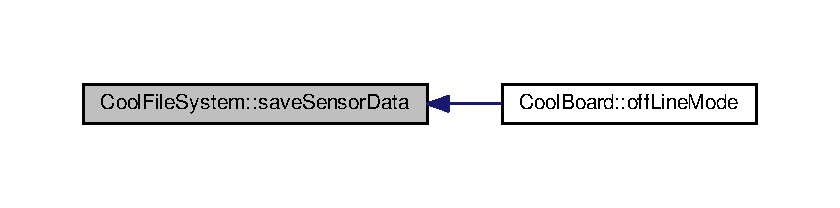
\includegraphics[width=350pt]{classCoolFileSystem_a4c560c2ddd40b74b7758e6ceb2c58957_icgraph}
\end{center}
\end{figure}
\mbox{\Hypertarget{classCoolFileSystem_a32dad79ae80182a83e2e8f52286b7c7b}\label{classCoolFileSystem_a32dad79ae80182a83e2e8f52286b7c7b}} 
\index{Cool\+File\+System@{Cool\+File\+System}!update\+Config\+Files@{update\+Config\+Files}}
\index{update\+Config\+Files@{update\+Config\+Files}!Cool\+File\+System@{Cool\+File\+System}}
\subsubsection{\texorpdfstring{update\+Config\+Files()}{updateConfigFiles()}}
{\footnotesize\ttfamily bool Cool\+File\+System\+::update\+Config\+Files (\begin{DoxyParamCaption}\item[{String}]{answer,  }\item[{int}]{J\+S\+O\+N\+\_\+\+S\+I\+ZE }\end{DoxyParamCaption})}

Cool\+File\+Syste\+::update\+Config\+Files( mqtt answer, answer size)\+: This method is provided to update the configuration files when the appropriate mqtt answer is received\+: -\/update \+: 1

\begin{DoxyReturn}{Returns}
true if the files are updated correctly, false otherwise 
\end{DoxyReturn}


Definition at line 94 of file Cool\+File\+System.\+cpp.



References temp.



Referenced by Cool\+Board\+::update().


\begin{DoxyCode}
95 \{
96     Serial.println(\textcolor{stringliteral}{"Entering CoolFileSystem.updateConfigFiles"});
97     Serial.println();
98 
99     \textcolor{comment}{//String conversion to char*}
100     \textcolor{comment}{//char jsonRoot = new char(answer.length() + 1);}
101     \textcolor{comment}{//strcpy(jsonRoot, answer.c\_str());}
102     \textcolor{comment}{//total json object }
103     DynamicJsonBuffer jsonBuffer(JSON\_SIZE);
104     JsonObject& root = jsonBuffer.parseObject( answer.c\_str() );
105     
106     \textcolor{keywordflow}{if}(! ( root.success() ))
107     \{
108         Serial.println(\textcolor{stringliteral}{"failed to parse root "});
109         Serial.println();
110         \textcolor{keywordflow}{return}(\textcolor{keyword}{false});
111     \}
112     \textcolor{keywordflow}{else}
113     \{
114         Serial.println(\textcolor{stringliteral}{"success to parse root "});
115         Serial.println();   
116     \}
117     
118     Serial.println(\textcolor{stringliteral}{"input message is : "});
119     root.printTo(Serial);
120     Serial.println();
121 
122     \textcolor{comment}{//temp string}
123     String \hyperlink{Irene3000_8h_a5905d48604152cf57aa6bfa087b49173}{temp};
124 
125     \textcolor{comment}{//CoolBoard Configuration File}
126 
127         JsonObject& jsonCoolBoard=root[\textcolor{stringliteral}{"CoolBoard"}];
128     \textcolor{keywordflow}{if}(jsonCoolBoard.success())
129     \{
130         File coolBoardConfig = SPIFFS.open(\textcolor{stringliteral}{"/coolBoardConfig.json"}, \textcolor{stringliteral}{"w"});   
131         \textcolor{keywordflow}{if}(!coolBoardConfig)
132         \{   
133             Serial.println(\textcolor{stringliteral}{"failed to write to coolBoardConfig.json"});
134             \textcolor{keywordflow}{return}(\textcolor{keyword}{false});
135         \}
136         Serial.println(\textcolor{stringliteral}{"CoolBoard Config"});
137         jsonCoolBoard.printTo(Serial);
138         
139         jsonCoolBoard.printTo(coolBoardConfig);
140         
141         coolBoardConfig.close();
142     \}
143     \textcolor{keywordflow}{else}
144     \{
145         Serial.println(\textcolor{stringliteral}{"failed to parse CoolBoard "});
146     \}       
147 
148     
149     \textcolor{comment}{//Cool Board Sensors Configuration File}
150     DynamicJsonBuffer jsonSBoard;
151         JsonObject& jsonSensorsBoard=root[\textcolor{stringliteral}{"CoolSensorsBoard"}];  
152     \textcolor{keywordflow}{if}(jsonSensorsBoard.success())
153     \{   
154         File coolBoardSensorsConfig = SPIFFS.open(\textcolor{stringliteral}{"/coolBoardSensorsConfig.json"}, \textcolor{stringliteral}{"w"}); 
155         \textcolor{keywordflow}{if}(!coolBoardSensorsConfig)
156         \{
157             Serial.println(\textcolor{stringliteral}{"failed to write coolBoardSensors.json"});
158             \textcolor{keywordflow}{return}(\textcolor{keyword}{false});
159         \}
160         
161         Serial.println(\textcolor{stringliteral}{"CoolBoardSensors Config"});
162         jsonSensorsBoard.printTo(coolBoardSensorsConfig);
163         jsonSensorsBoard.printTo(Serial);
164         coolBoardSensorsConfig.close();
165     \}
166     \textcolor{keywordflow}{else}
167     \{
168         Serial.println(\textcolor{stringliteral}{"failed to parse CoolSensorsBoard sensors "});    
169     \}
170     
171     
172     
173     \textcolor{comment}{//rtc configuration file}
174     DynamicJsonBuffer jsonR;
175         JsonObject& jsonRTC=root[\textcolor{stringliteral}{"rtc"}];
176     Serial.println(\textcolor{stringliteral}{"before config rtc json"});
177     jsonRTC.printTo(Serial);
178     \textcolor{keywordflow}{if}(jsonRTC.success() )
179     \{
180         File rtcConfig = SPIFFS.open(\textcolor{stringliteral}{"/rtcConfig.json"}, \textcolor{stringliteral}{"w"});   
181         \textcolor{keywordflow}{if}(!rtcConfig)
182         \{
183             Serial.println(\textcolor{stringliteral}{"failed to write rtcConfig.json"});
184             \textcolor{keywordflow}{return}(\textcolor{keyword}{false});
185         \}
186         Serial.println(\textcolor{stringliteral}{"RTC Config"});
187         jsonRTC.printTo(rtcConfig);
188         jsonRTC.printTo(Serial);
189         rtcConfig.close();
190     
191     \}
192     \textcolor{keywordflow}{else}
193     \{
194         Serial.println(\textcolor{stringliteral}{"failed to parse rtc "});
195     \}
196 
197     
198     
199     
200     
201         \textcolor{comment}{//cool board led configuration}
202     DynamicJsonBuffer jsonLBoard;
203         JsonObject& jsonLedBoard=root[\textcolor{stringliteral}{"led"}];
204     Serial.println(\textcolor{stringliteral}{"before config Led json"});
205     jsonLedBoard.printTo(Serial);
206     \textcolor{keywordflow}{if}(jsonLedBoard.success())
207     \{   
208         File coolBoardLedConfig = SPIFFS.open(\textcolor{stringliteral}{"/coolBoardLedConfig.json"}, \textcolor{stringliteral}{"w"}); 
209         \textcolor{keywordflow}{if}(!coolBoardLedConfig)
210         \{
211             Serial.println(\textcolor{stringliteral}{"failed to write led config"});
212             \textcolor{keywordflow}{return}(\textcolor{keyword}{false});
213         \}
214         Serial.println(\textcolor{stringliteral}{"CoolBoardLed Config"});
215         jsonLedBoard.printTo(coolBoardLedConfig);
216         jsonLedBoard.printTo(Serial);
217         coolBoardLedConfig.close();
218     
219     \}
220     \textcolor{keywordflow}{else}
221     \{
222         Serial.println(\textcolor{stringliteral}{"failed to parse led"});
223     \}
224         
225 
226     
227 
228     \textcolor{comment}{//jetpack configuration}
229     DynamicJsonBuffer jsonJBoard;
230         JsonObject& jsonJetpack=root[\textcolor{stringliteral}{"jetPack"}];
231     Serial.println(\textcolor{stringliteral}{"before config jetpack json"});
232     jsonJetpack.printTo(Serial);
233     \textcolor{keywordflow}{if}(jsonJetpack.success())
234     \{   
235         File jetPackConfig = SPIFFS.open(\textcolor{stringliteral}{"/jetPackConfig.json"}, \textcolor{stringliteral}{"w"});   
236         \textcolor{keywordflow}{if}(!jetPackConfig)
237         \{
238             Serial.println(\textcolor{stringliteral}{"failed to write jetpack file"});
239             \textcolor{keywordflow}{return}(\textcolor{keyword}{false});
240         \}
241         Serial.println(\textcolor{stringliteral}{"jetpack Config"});   
242         jsonJetpack.printTo(jetPackConfig);
243         jsonJetpack.printTo(Serial);
244         jetPackConfig.close();
245     \}
246     \textcolor{keywordflow}{else}
247     \{
248         Serial.println(\textcolor{stringliteral}{"failed to parse jetpack"});  
249     \}
250     
251     \textcolor{comment}{//irene configuration   }
252     DynamicJsonBuffer jsonIBoard;
253         JsonObject& jsonIrene=root[\textcolor{stringliteral}{"irene3000"}];
254     Serial.println(\textcolor{stringliteral}{"before config irene json"}); 
255     jsonIrene.printTo(Serial);
256     \textcolor{keywordflow}{if}(jsonIrene.success())
257     \{
258         File irene3000Config = SPIFFS.open(\textcolor{stringliteral}{"/irene3000Config.json"}, \textcolor{stringliteral}{"w"});   
259         \textcolor{keywordflow}{if}(!irene3000Config)
260         \{
261             Serial.println(\textcolor{stringliteral}{"failed to write irene file"});
262             \textcolor{keywordflow}{return}(\textcolor{keyword}{false});
263         \}
264         Serial.println(\textcolor{stringliteral}{"irene3000 Config"});
265         jsonIrene.printTo(irene3000Config);
266         jsonIrene.printTo(Serial);
267         irene3000Config.close();
268     
269     \}
270     \textcolor{keywordflow}{else}
271     \{
272         Serial.println(\textcolor{stringliteral}{"failed to parse irene"});    
273     \}
274     
275     \textcolor{comment}{//external sensors}
276     DynamicJsonBuffer jsonESBoard;
277         JsonObject& jsonExternalSensors=root[\textcolor{stringliteral}{"externalSensors"}];
278     Serial.println(\textcolor{stringliteral}{"before config external Sensors json"});
279     jsonExternalSensors.printTo(Serial);
280     \textcolor{keywordflow}{if}(jsonExternalSensors.success())
281     \{
282         File externalSensorsConfig = SPIFFS.open(\textcolor{stringliteral}{"/externalSensorsConfig.json"}, \textcolor{stringliteral}{"w"});   
283         \textcolor{keywordflow}{if}(!externalSensorsConfig)
284         \{
285             Serial.println(\textcolor{stringliteral}{"failed to open external sensors file "});
286             \textcolor{keywordflow}{return}(\textcolor{keyword}{false});
287         \}
288         Serial.println(\textcolor{stringliteral}{"externalSensors Config"});
289         jsonExternalSensors.printTo(externalSensorsConfig);
290         jsonExternalSensors.printTo(Serial);
291     
292         externalSensorsConfig.close();
293 
294     \}
295     \textcolor{keywordflow}{else}
296     \{
297         Serial.println(\textcolor{stringliteral}{"failed to parse external sensors"}); 
298     \}
299 
300     
301     \textcolor{comment}{//mqtt config}
302     DynamicJsonBuffer jsonMQ;
303         JsonObject& jsonMQTT=root[\textcolor{stringliteral}{"mqtt"}];
304     Serial.println(\textcolor{stringliteral}{"before config mqtt json"});
305     jsonMQTT.printTo(Serial);
306     \textcolor{keywordflow}{if}(jsonMQTT.success())
307     \{
308         File mqttConfig = SPIFFS.open(\textcolor{stringliteral}{"/mqttConfig.json"}, \textcolor{stringliteral}{"w"}); 
309         \textcolor{keywordflow}{if}(!mqttConfig)
310         \{
311             Serial.println(\textcolor{stringliteral}{"failed to open mqtt file "});        
312             \textcolor{keywordflow}{return}(\textcolor{keyword}{false});
313         \}
314         Serial.println(\textcolor{stringliteral}{"mqtt config"});
315         jsonMQTT.printTo(mqttConfig);
316         jsonMQTT.printTo(Serial);
317         mqttConfig.close();
318     \}
319     \textcolor{keywordflow}{else}
320     \{
321         Serial.println(\textcolor{stringliteral}{"failed to parse mqtt"}); 
322     \}   
323         
324     \textcolor{keywordflow}{return} \textcolor{keyword}{true};
325 
326 \}   
\end{DoxyCode}
Here is the caller graph for this function\+:\nopagebreak
\begin{figure}[H]
\begin{center}
\leavevmode
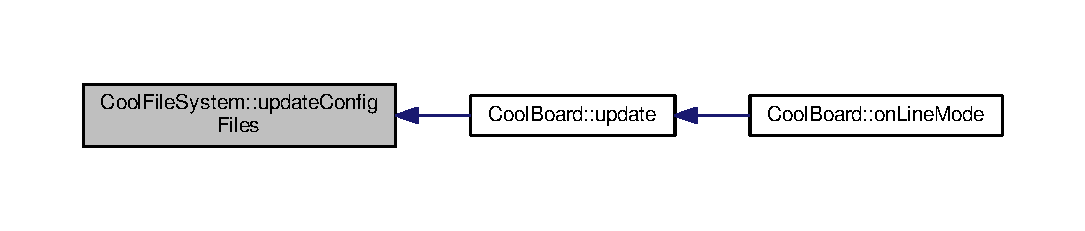
\includegraphics[width=350pt]{classCoolFileSystem_a32dad79ae80182a83e2e8f52286b7c7b_icgraph}
\end{center}
\end{figure}


\subsection{Member Data Documentation}
\mbox{\Hypertarget{classCoolFileSystem_ad398e0c5c41a0c88acdf5d672aa71351}\label{classCoolFileSystem_ad398e0c5c41a0c88acdf5d672aa71351}} 
\index{Cool\+File\+System@{Cool\+File\+System}!saved\+Data@{saved\+Data}}
\index{saved\+Data@{saved\+Data}!Cool\+File\+System@{Cool\+File\+System}}
\subsubsection{\texorpdfstring{saved\+Data}{savedData}}
{\footnotesize\ttfamily bool Cool\+File\+System\+::saved\+Data =0\hspace{0.3cm}{\ttfamily [private]}}



Definition at line 38 of file Cool\+File\+System.\+h.



Referenced by get\+Sensor\+Saved\+Data(), is\+Data\+Saved(), and save\+Sensor\+Data().



The documentation for this class was generated from the following files\+:\begin{DoxyCompactItemize}
\item 
/home/ashiroji/\+Arduino/libraries/\+Cool\+Board/\hyperlink{CoolFileSystem_8h}{Cool\+File\+System.\+h}\item 
/home/ashiroji/\+Arduino/libraries/\+Cool\+Board/\hyperlink{CoolFileSystem_8cpp}{Cool\+File\+System.\+cpp}\end{DoxyCompactItemize}

\hypertarget{classCoolMQTT}{}\section{Cool\+M\+Q\+TT Class Reference}
\label{classCoolMQTT}\index{Cool\+M\+Q\+TT@{Cool\+M\+Q\+TT}}


This class handles the mqtt client.  




{\ttfamily \#include $<$Cool\+M\+Q\+T\+T.\+h$>$}



Collaboration diagram for Cool\+M\+Q\+TT\+:\nopagebreak
\begin{figure}[H]
\begin{center}
\leavevmode
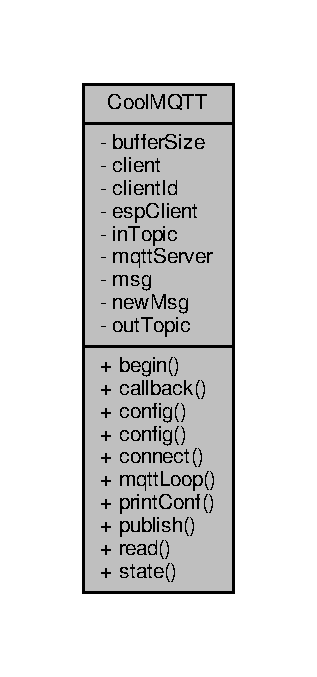
\includegraphics[width=177pt]{classCoolMQTT__coll__graph}
\end{center}
\end{figure}
\subsection*{Public Member Functions}
\begin{DoxyCompactItemize}
\item 
void \hyperlink{classCoolMQTT_ac9248808641ebf3054ed0620ea9d0100}{begin} ()
\item 
int \hyperlink{classCoolMQTT_a58b0b1f64b269c2681685208262fba1d}{connect} (uint16\+\_\+t keep\+Alive)
\item 
bool \hyperlink{classCoolMQTT_ace977b3e90ab14b1199fe5c4fb0a13ec}{publish} (const char $\ast$data)
\item 
bool \hyperlink{classCoolMQTT_a65a506641740ce797ceadd4fa8a286d3}{publish} (const char $\ast$data, int log\+Interval)
\item 
String \hyperlink{classCoolMQTT_ae3c18f6ae9723746d32765f1c8f176ca}{read} ()
\item 
void \hyperlink{classCoolMQTT_a9b703de4f1358f0ee7a5e8c44979c648}{config} (const char \hyperlink{classCoolMQTT_ab8bb951f87ddbf92db74c2ad16a3e53e}{mqtt\+Server}\mbox{[}$\,$\mbox{]}, const char \hyperlink{classCoolMQTT_a4492f52a441e83cc5151010317fdb52d}{in\+Topic}\mbox{[}$\,$\mbox{]}, const char \hyperlink{classCoolMQTT_a109c786a17b463f9eeba046194279522}{out\+Topic}\mbox{[}$\,$\mbox{]}, const char \hyperlink{classCoolMQTT_a8cd47e45d457f908d4b4390b35aaee83}{user}\mbox{[}$\,$\mbox{]}, int \hyperlink{classCoolMQTT_a7f3cf26b51d6770f216e42c5ef13ca9f}{buffer\+Size})
\item 
bool \hyperlink{classCoolMQTT_a6571671781a505feca9a8a56e256c6bc}{config} ()
\item 
void \hyperlink{classCoolMQTT_a30d82ad665bfb603f46ecdbc290775df}{callback} (char $\ast$topic, byte $\ast$payload, unsigned int length)
\item 
void \hyperlink{classCoolMQTT_a40553a0ad4b5ecf1cb4411ab54ca85fb}{print\+Conf} ()
\item 
int \hyperlink{classCoolMQTT_a5d003307eff78efbd585e42b43b72b6d}{state} ()
\item 
bool \hyperlink{classCoolMQTT_aa5eaae967b562b62cbcf2b8d81f6e5d5}{mqtt\+Loop} ()
\item 
String \hyperlink{classCoolMQTT_a373cc92fca7760d886f02d8a6e5b3f63}{get\+User} ()
\end{DoxyCompactItemize}
\subsection*{Private Attributes}
\begin{DoxyCompactItemize}
\item 
char \hyperlink{classCoolMQTT_ab8bb951f87ddbf92db74c2ad16a3e53e}{mqtt\+Server} \mbox{[}50\mbox{]} =\{\textquotesingle{}0\textquotesingle{}\}
\item 
String \hyperlink{classCoolMQTT_af6b19e7074dbbb4ae493c44dcb53f7ff}{msg} =\char`\"{}\char`\"{}
\item 
char \hyperlink{classCoolMQTT_a4492f52a441e83cc5151010317fdb52d}{in\+Topic} \mbox{[}50\mbox{]} =\{\textquotesingle{}0\textquotesingle{}\}
\item 
char \hyperlink{classCoolMQTT_a109c786a17b463f9eeba046194279522}{out\+Topic} \mbox{[}50\mbox{]} =\{\textquotesingle{}0\textquotesingle{}\}
\item 
char \hyperlink{classCoolMQTT_a8cd47e45d457f908d4b4390b35aaee83}{user} \mbox{[}50\mbox{]} =\{\textquotesingle{}0\textquotesingle{}\}
\item 
int \hyperlink{classCoolMQTT_a7f3cf26b51d6770f216e42c5ef13ca9f}{buffer\+Size} =3000
\item 
Wi\+Fi\+Client \hyperlink{classCoolMQTT_acc30a0200967374a524092a8a806502a}{esp\+Client}
\item 
Pub\+Sub\+Client \hyperlink{classCoolMQTT_a4ca71e4f76ef868692a297efd45b1415}{client}
\item 
bool \hyperlink{classCoolMQTT_a3240388137b885775aadf38e96b24c6b}{new\+Msg} =0
\item 
unsigned long \hyperlink{classCoolMQTT_a3db37ef9ed3b05b2a8d44edba0e7d3cc}{previous\+Log\+Time} =0
\end{DoxyCompactItemize}


\subsection{Detailed Description}
This class handles the mqtt client. 

Definition at line 22 of file Cool\+M\+Q\+T\+T.\+h.



\subsection{Member Function Documentation}
\mbox{\Hypertarget{classCoolMQTT_ac9248808641ebf3054ed0620ea9d0100}\label{classCoolMQTT_ac9248808641ebf3054ed0620ea9d0100}} 
\index{Cool\+M\+Q\+TT@{Cool\+M\+Q\+TT}!begin@{begin}}
\index{begin@{begin}!Cool\+M\+Q\+TT@{Cool\+M\+Q\+TT}}
\subsubsection{\texorpdfstring{begin()}{begin()}}
{\footnotesize\ttfamily void Cool\+M\+Q\+T\+T\+::begin (\begin{DoxyParamCaption}{ }\end{DoxyParamCaption})}

\hyperlink{classCoolMQTT_ac9248808641ebf3054ed0620ea9d0100}{Cool\+M\+Q\+T\+T\+::begin()}\+: This method is provided to set the mqtt client\textquotesingle{}s parameters\+: -\/client -\/server -\/callback method -\/buffer size 

Definition at line 39 of file Cool\+M\+Q\+T\+T.\+cpp.



References buffer\+Size, callback(), client, esp\+Client, and mqtt\+Server.



Referenced by Cool\+Board\+::begin().


\begin{DoxyCode}
40 \{ 
41 
42 \textcolor{preprocessor}{#if DEBUG == 1 }
43 
44     Serial.println( F(\textcolor{stringliteral}{"Entering CoolMQTT.begin()"}) );
45     Serial.println();
46 
47 \textcolor{preprocessor}{#endif}
48 
49     \hyperlink{classCoolMQTT_a4ca71e4f76ef868692a297efd45b1415}{client}.setClient(\hyperlink{classCoolMQTT_acc30a0200967374a524092a8a806502a}{espClient});
50     \hyperlink{classCoolMQTT_a4ca71e4f76ef868692a297efd45b1415}{client}.setServer(\hyperlink{classCoolMQTT_ab8bb951f87ddbf92db74c2ad16a3e53e}{mqttServer}, 1883); 
51     \hyperlink{classCoolMQTT_a4ca71e4f76ef868692a297efd45b1415}{client}.setCallback([\textcolor{keyword}{this}] (\textcolor{keywordtype}{char}* topic, byte* payload, \textcolor{keywordtype}{unsigned} \textcolor{keywordtype}{int} length) \{ this->
      \hyperlink{classCoolMQTT_a30d82ad665bfb603f46ecdbc290775df}{callback}(topic, payload, length); \});
52     \hyperlink{classCoolMQTT_a4ca71e4f76ef868692a297efd45b1415}{client}.setBufferSize((\textcolor{keywordtype}{unsigned} \textcolor{keywordtype}{short})\hyperlink{classCoolMQTT_a7f3cf26b51d6770f216e42c5ef13ca9f}{bufferSize});
53 
54 \}
\end{DoxyCode}
Here is the call graph for this function\+:\nopagebreak
\begin{figure}[H]
\begin{center}
\leavevmode
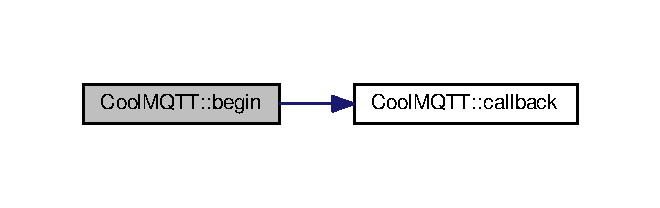
\includegraphics[width=317pt]{classCoolMQTT_ac9248808641ebf3054ed0620ea9d0100_cgraph}
\end{center}
\end{figure}
Here is the caller graph for this function\+:
\nopagebreak
\begin{figure}[H]
\begin{center}
\leavevmode
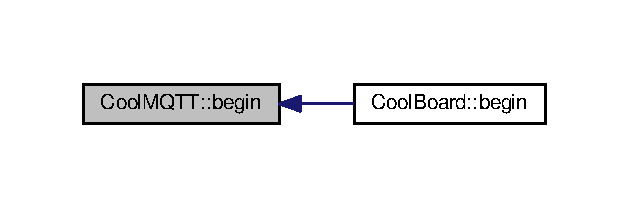
\includegraphics[width=302pt]{classCoolMQTT_ac9248808641ebf3054ed0620ea9d0100_icgraph}
\end{center}
\end{figure}
\mbox{\Hypertarget{classCoolMQTT_a30d82ad665bfb603f46ecdbc290775df}\label{classCoolMQTT_a30d82ad665bfb603f46ecdbc290775df}} 
\index{Cool\+M\+Q\+TT@{Cool\+M\+Q\+TT}!callback@{callback}}
\index{callback@{callback}!Cool\+M\+Q\+TT@{Cool\+M\+Q\+TT}}
\subsubsection{\texorpdfstring{callback()}{callback()}}
{\footnotesize\ttfamily void Cool\+M\+Q\+T\+T\+::callback (\begin{DoxyParamCaption}\item[{char $\ast$}]{topic,  }\item[{byte $\ast$}]{payload,  }\item[{unsigned int}]{length }\end{DoxyParamCaption})}

Cool\+M\+Q\+T\+T\+::callback(in topic, incoming message , message length)\+: This method is provided to handle incoming messages from the subscribed in\+Topic.

Arguments are automatically assigned in client.\+set\+Callback() 

Definition at line 279 of file Cool\+M\+Q\+T\+T.\+cpp.



References msg, new\+Msg, and temp.



Referenced by begin().


\begin{DoxyCode}
280 \{
281 
282 \textcolor{preprocessor}{#if DEBUG == 1}
283 
284     Serial.println( F(\textcolor{stringliteral}{"Entering CoolMQTT.callback() "}) );
285     Serial.println();
286 
287 \textcolor{preprocessor}{#endif }
288 
289     \textcolor{keywordflow}{if}(this->\hyperlink{classCoolMQTT_a3240388137b885775aadf38e96b24c6b}{newMsg}==\textcolor{keyword}{false})
290     \{
291         \textcolor{keywordtype}{char} \hyperlink{Irene3000_8h_a5905d48604152cf57aa6bfa087b49173}{temp}[length+1];
292 
293 \textcolor{preprocessor}{    #if DEBUG == 1}
294 
295         Serial.println( F(\textcolor{stringliteral}{"received temp msg : "}) );
296         
297 \textcolor{preprocessor}{    #endif}
298         
299         \textcolor{keywordflow}{for} (\textcolor{keywordtype}{int} i = 0; i < length; i++) 
300         \{
301             temp[i]=(char)payload[i];
302         
303 \textcolor{preprocessor}{        #if DEBUG == 1 }
304 
305             Serial.print( (\textcolor{keywordtype}{char})payload[i] );
306         
307 \textcolor{preprocessor}{        #endif}
308 
309         \}
310     
311 \textcolor{preprocessor}{    #if DEBUG == 1 }
312 
313         Serial.println();
314         Serial.println( F(\textcolor{stringliteral}{"storing new message : "}) );
315 
316         Serial.print(F(\textcolor{stringliteral}{"length : "}));
317         Serial.println(length);
318         
319         Serial.print(F(\textcolor{stringliteral}{"size : "}));
320         Serial.print(\textcolor{keyword}{sizeof}(payload));
321         Serial.println();
322     
323 \textcolor{preprocessor}{    #endif}
324 
325         this->\hyperlink{classCoolMQTT_a3240388137b885775aadf38e96b24c6b}{newMsg}=\textcolor{keyword}{true};
326 
327         temp[length+1]=\textcolor{charliteral}{'\(\backslash\)0'};
328 
329         this->\hyperlink{classCoolMQTT_af6b19e7074dbbb4ae493c44dcb53f7ff}{msg}=String(temp);
330         this->\hyperlink{classCoolMQTT_af6b19e7074dbbb4ae493c44dcb53f7ff}{msg}.remove(length,1);
331     
332 \textcolor{preprocessor}{    #if DEBUG == 1 }
333 
334         Serial.println( F(\textcolor{stringliteral}{"stored message : "}) );
335         Serial.println(this->\hyperlink{classCoolMQTT_af6b19e7074dbbb4ae493c44dcb53f7ff}{msg});
336     
337 \textcolor{preprocessor}{    #endif}
338 
339     \}
340     \textcolor{keywordflow}{else}
341     \{
342     
343 \textcolor{preprocessor}{    #if DEBUG == 1}
344 
345         Serial.println( F(\textcolor{stringliteral}{"did not read last message"}) );
346     
347 \textcolor{preprocessor}{    #endif }
348         
349     \}
350 
351 \}
\end{DoxyCode}
Here is the caller graph for this function\+:
\nopagebreak
\begin{figure}[H]
\begin{center}
\leavevmode
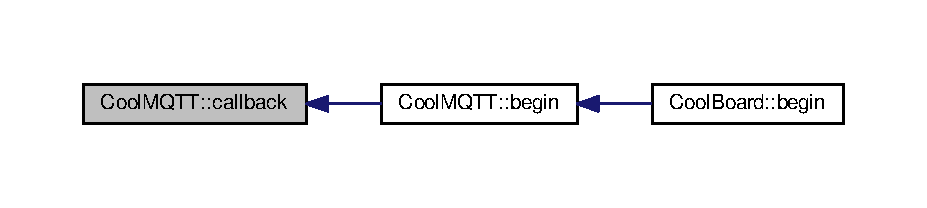
\includegraphics[width=350pt]{classCoolMQTT_a30d82ad665bfb603f46ecdbc290775df_icgraph}
\end{center}
\end{figure}
\mbox{\Hypertarget{classCoolMQTT_a9b703de4f1358f0ee7a5e8c44979c648}\label{classCoolMQTT_a9b703de4f1358f0ee7a5e8c44979c648}} 
\index{Cool\+M\+Q\+TT@{Cool\+M\+Q\+TT}!config@{config}}
\index{config@{config}!Cool\+M\+Q\+TT@{Cool\+M\+Q\+TT}}
\subsubsection{\texorpdfstring{config()}{config()}\hspace{0.1cm}{\footnotesize\ttfamily [1/2]}}
{\footnotesize\ttfamily void Cool\+M\+Q\+T\+T\+::config (\begin{DoxyParamCaption}\item[{const char}]{mqtt\+Server\mbox{[}$\,$\mbox{]},  }\item[{const char}]{in\+Topic\mbox{[}$\,$\mbox{]},  }\item[{const char}]{out\+Topic\mbox{[}$\,$\mbox{]},  }\item[{const char}]{user\mbox{[}$\,$\mbox{]},  }\item[{int}]{buffer\+Size }\end{DoxyParamCaption})}

Cool\+M\+Q\+T\+T\+::config(server,in topic, out topic , user Id, buffer size)\+: This method is provided to manually configure the mqtt client 

Definition at line 596 of file Cool\+M\+Q\+T\+T.\+cpp.



References buffer\+Size.



Referenced by Cool\+Board\+::begin().


\begin{DoxyCode}
597 \{
598 
599 \textcolor{preprocessor}{#if DEBUG == 1}
600 
601     Serial.println( F(\textcolor{stringliteral}{"Entering CoolMQTT.config() , no SPIFFS variant"}) );
602     Serial.println();
603 
604 \textcolor{preprocessor}{#endif}
605 
606     \textcolor{keywordflow}{for}(\textcolor{keywordtype}{int} i =0;i< 50 ;i++)
607     \{
608         this->\hyperlink{classCoolMQTT_ab8bb951f87ddbf92db74c2ad16a3e53e}{mqttServer}[i]=\hyperlink{classCoolMQTT_ab8bb951f87ddbf92db74c2ad16a3e53e}{mqttServer}[i];
609         this->\hyperlink{classCoolMQTT_a4492f52a441e83cc5151010317fdb52d}{inTopic}[i]=\hyperlink{classCoolMQTT_a4492f52a441e83cc5151010317fdb52d}{inTopic}[i];
610         this->\hyperlink{classCoolMQTT_a109c786a17b463f9eeba046194279522}{outTopic}[i]=\hyperlink{classCoolMQTT_a109c786a17b463f9eeba046194279522}{outTopic}[i];
611         this->\hyperlink{classCoolMQTT_a8cd47e45d457f908d4b4390b35aaee83}{user}[i]=\hyperlink{classCoolMQTT_a8cd47e45d457f908d4b4390b35aaee83}{user}[i];
612     \}
613     this->\hyperlink{classCoolMQTT_a7f3cf26b51d6770f216e42c5ef13ca9f}{bufferSize}=\hyperlink{classCoolMQTT_a7f3cf26b51d6770f216e42c5ef13ca9f}{bufferSize};
614     
615 
616 \}
\end{DoxyCode}
Here is the caller graph for this function\+:
\nopagebreak
\begin{figure}[H]
\begin{center}
\leavevmode
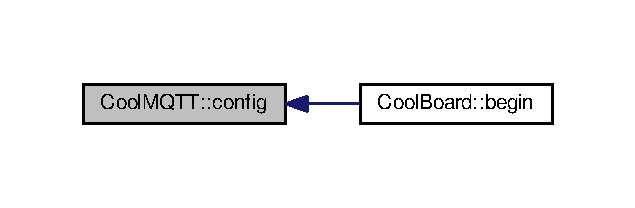
\includegraphics[width=305pt]{classCoolMQTT_a9b703de4f1358f0ee7a5e8c44979c648_icgraph}
\end{center}
\end{figure}
\mbox{\Hypertarget{classCoolMQTT_a6571671781a505feca9a8a56e256c6bc}\label{classCoolMQTT_a6571671781a505feca9a8a56e256c6bc}} 
\index{Cool\+M\+Q\+TT@{Cool\+M\+Q\+TT}!config@{config}}
\index{config@{config}!Cool\+M\+Q\+TT@{Cool\+M\+Q\+TT}}
\subsubsection{\texorpdfstring{config()}{config()}\hspace{0.1cm}{\footnotesize\ttfamily [2/2]}}
{\footnotesize\ttfamily bool Cool\+M\+Q\+T\+T\+::config (\begin{DoxyParamCaption}{ }\end{DoxyParamCaption})}

\hyperlink{classCoolMQTT_a6571671781a505feca9a8a56e256c6bc}{Cool\+M\+Q\+T\+T\+::config()}\+: This method is provided to configure the mqtt\+Client \+: -\/server -\/in\+Topic -\/out\+Topic -\/client Id -\/buffer size

\begin{DoxyReturn}{Returns}
true if successful,false otherwise 
\end{DoxyReturn}


Definition at line 399 of file Cool\+M\+Q\+T\+T.\+cpp.



References buffer\+Size, in\+Topic, mqtt\+Server, out\+Topic, and user.


\begin{DoxyCode}
400 \{
401 
402 \textcolor{preprocessor}{#if DEBUG == 1 }
403 
404     Serial.println( F(\textcolor{stringliteral}{"Entering CoolMQTT.config()"}) );
405     Serial.println();
406 
407 \textcolor{preprocessor}{#endif}
408 
409     \textcolor{comment}{//read config file}
410     \textcolor{comment}{//update data}
411     File configFile = SPIFFS.open(\textcolor{stringliteral}{"/mqttConfig.json"}, \textcolor{stringliteral}{"r"});
412 
413     \textcolor{keywordflow}{if} (!configFile) 
414     \{
415     
416 \textcolor{preprocessor}{    #if DEBUG == 1 }
417 
418         Serial.println( F(\textcolor{stringliteral}{"failed to read /mqttConfig.json"}) );
419         Serial.println();
420 
421 \textcolor{preprocessor}{    #endif}
422 
423         \textcolor{keywordflow}{return}(\textcolor{keyword}{false});
424     \}
425     \textcolor{keywordflow}{else}
426     \{
427         \textcolor{keywordtype}{size\_t} size = configFile.size();
428         \textcolor{comment}{// Allocate a buffer to store contents of the file.}
429         std::unique\_ptr<char[]> buf(\textcolor{keyword}{new} \textcolor{keywordtype}{char}[size]);
430 
431         configFile.readBytes(buf.get(), size);
432         DynamicJsonBuffer jsonBuffer;
433         JsonObject& json = jsonBuffer.parseObject(buf.get());
434         \textcolor{keywordflow}{if} (!json.success()) 
435         \{
436         
437 \textcolor{preprocessor}{        #if DEBUG == 1 }
438 
439             Serial.println( F(\textcolor{stringliteral}{"failed to parse json "}) );
440             Serial.println();
441         
442 \textcolor{preprocessor}{        #endif}
443             
444             \textcolor{keywordflow}{return}(\textcolor{keyword}{false});
445         \} 
446         \textcolor{keywordflow}{else}
447         \{
448         
449 \textcolor{preprocessor}{        #if DEBUG == 1 }
450         
451             Serial.println( F(\textcolor{stringliteral}{"configuration json is "}) );
452             json.printTo(Serial);
453             Serial.println();
454 
455             Serial.print(F(\textcolor{stringliteral}{"jsonBuffer size: "}));
456             Serial.println(jsonBuffer.size());
457             Serial.println();
458 
459 
460 \textcolor{preprocessor}{        #endif}
461 
462             \textcolor{keywordflow}{if}(json[\textcolor{stringliteral}{"mqttServer"}].success() )
463             \{           
464                 \textcolor{keyword}{const} \textcolor{keywordtype}{char}* tempmqttServer = json[\textcolor{stringliteral}{"mqttServer"}]; 
465                 \textcolor{keywordflow}{for}(\textcolor{keywordtype}{int} i =0;i< 50 ;i++)
466                 \{
467                     \hyperlink{classCoolMQTT_ab8bb951f87ddbf92db74c2ad16a3e53e}{mqttServer}[i]=tempmqttServer[i];
468                 \}
469             \}
470             \textcolor{keywordflow}{else}
471             \{
472                 \textcolor{keywordflow}{for}(\textcolor{keywordtype}{int} i =0;i< 50 ;i++)
473                 \{
474                     this->\hyperlink{classCoolMQTT_ab8bb951f87ddbf92db74c2ad16a3e53e}{mqttServer}[i]=this->\hyperlink{classCoolMQTT_ab8bb951f87ddbf92db74c2ad16a3e53e}{mqttServer}[i];
475                 \}
476 
477             \}
478             json[\textcolor{stringliteral}{"mqttServer"}]=this->\hyperlink{classCoolMQTT_ab8bb951f87ddbf92db74c2ad16a3e53e}{mqttServer};
479 
480             
481             \textcolor{keywordflow}{if}(json[\textcolor{stringliteral}{"inTopic"}].success() )
482             \{
483                 \textcolor{keyword}{const} \textcolor{keywordtype}{char}* tempInTopic = json[\textcolor{stringliteral}{"inTopic"}]; 
484                 \textcolor{keywordflow}{for}(\textcolor{keywordtype}{int} i =0;i< 50;i++)
485                 \{
486                     \hyperlink{classCoolMQTT_a4492f52a441e83cc5151010317fdb52d}{inTopic}[i]=tempInTopic[i];
487                 \}
488             \}
489             \textcolor{keywordflow}{else}
490             \{
491                 String tempMAC = WiFi.macAddress();
492                 tempMAC.replace(\textcolor{stringliteral}{":"},\textcolor{stringliteral}{""});
493                 snprintf(\hyperlink{classCoolMQTT_a4492f52a441e83cc5151010317fdb52d}{inTopic}, 50, \textcolor{stringliteral}{"$aws/things/%s/shadow/update/delta"}, tempMAC.c\_str());    
494             
495 \textcolor{preprocessor}{            #if DEBUG == 1              }
496                 
497                 Serial.print( F(\textcolor{stringliteral}{"Set Incomming MQTT Channel to : "}) );
498                 Serial.println(\hyperlink{classCoolMQTT_a4492f52a441e83cc5151010317fdb52d}{inTopic});
499             
500 \textcolor{preprocessor}{            #endif  }
501 
502             \}
503             json[\textcolor{stringliteral}{"inTopic"}]=this->\hyperlink{classCoolMQTT_a4492f52a441e83cc5151010317fdb52d}{inTopic};
504             
505             
506             \textcolor{keywordflow}{if}(json[\textcolor{stringliteral}{"outTopic"}].success() )
507             \{
508                 \textcolor{keyword}{const} \textcolor{keywordtype}{char}* tempOutTopic = json[\textcolor{stringliteral}{"outTopic"}]; 
509                 \textcolor{keywordflow}{for}(\textcolor{keywordtype}{int} i =0;i<50;i++)
510                 \{
511                     \hyperlink{classCoolMQTT_a109c786a17b463f9eeba046194279522}{outTopic}[i]=tempOutTopic[i];
512                 \}
513             \}
514             \textcolor{keywordflow}{else}
515             \{
516                 String tempMAC = WiFi.macAddress();
517                 tempMAC.replace(\textcolor{stringliteral}{":"},\textcolor{stringliteral}{""});
518                 snprintf(\hyperlink{classCoolMQTT_a109c786a17b463f9eeba046194279522}{outTopic}, 50, \textcolor{stringliteral}{"$aws/things/%s/shadow/update"}, tempMAC.c\_str());
519             
520 \textcolor{preprocessor}{            #if DEBUG == 1 }
521 
522                 Serial.print( F(\textcolor{stringliteral}{"Set Outgoing MQTT Channel to : "}) );
523                 Serial.println(\hyperlink{classCoolMQTT_a109c786a17b463f9eeba046194279522}{outTopic});
524             
525 \textcolor{preprocessor}{            #endif}
526 
527             \}
528             json[\textcolor{stringliteral}{"outTopic"}]=this->\hyperlink{classCoolMQTT_a109c786a17b463f9eeba046194279522}{outTopic};
529         
530             
531             \textcolor{keywordflow}{if}(json[\textcolor{stringliteral}{"user"}].success() )
532             \{               
533                 \textcolor{keyword}{const} \textcolor{keywordtype}{char}* tempUser = json[\textcolor{stringliteral}{"user"}]; 
534                 \textcolor{keywordflow}{for}(\textcolor{keywordtype}{int} i =0;i<50;i++)
535                 \{
536                     \hyperlink{classCoolMQTT_a8cd47e45d457f908d4b4390b35aaee83}{user}[i]=tempUser[i];
537                 \}
538             \}
539             \textcolor{keywordflow}{else}
540             \{
541                 \textcolor{keywordflow}{for}(\textcolor{keywordtype}{int} i=0;i<50;i++)
542                 \{
543                     this->\hyperlink{classCoolMQTT_a8cd47e45d457f908d4b4390b35aaee83}{user}[i]=this->\hyperlink{classCoolMQTT_a8cd47e45d457f908d4b4390b35aaee83}{user}[i];
544                 \}               
545             \}
546             json[\textcolor{stringliteral}{"user"}]=this->\hyperlink{classCoolMQTT_a8cd47e45d457f908d4b4390b35aaee83}{user};
547             
548             \textcolor{keywordflow}{if}(json[\textcolor{stringliteral}{"bufferSize"}].success() )
549             \{
550                 \textcolor{keywordtype}{int} tempBufferSize = json[\textcolor{stringliteral}{"bufferSize"}]; 
551                 \hyperlink{classCoolMQTT_a7f3cf26b51d6770f216e42c5ef13ca9f}{bufferSize}=tempBufferSize;
552             \}
553             \textcolor{keywordflow}{else}
554             \{
555                 this->\hyperlink{classCoolMQTT_a7f3cf26b51d6770f216e42c5ef13ca9f}{bufferSize}=this->\hyperlink{classCoolMQTT_a7f3cf26b51d6770f216e42c5ef13ca9f}{bufferSize};
556             \}
557             json[\textcolor{stringliteral}{"bufferSize"}]=this->\hyperlink{classCoolMQTT_a7f3cf26b51d6770f216e42c5ef13ca9f}{bufferSize};
558 
559             configFile.close();
560             configFile = SPIFFS.open(\textcolor{stringliteral}{"/mqttConfig.json"}, \textcolor{stringliteral}{"w"});
561             \textcolor{keywordflow}{if}(!configFile)
562             \{
563             
564 \textcolor{preprocessor}{            #if DEBUG == 1 }
565 
566                 Serial.println( F(\textcolor{stringliteral}{"failed to write to /mqttConfig.json"}) );
567             
568 \textcolor{preprocessor}{            #endif}
569 
570                 \textcolor{keywordflow}{return}(\textcolor{keyword}{false});              
571             \}
572             
573             json.printTo(configFile);
574             configFile.close();
575 
576 \textcolor{preprocessor}{        #if DEBUG == 1 }
577 
578             Serial.println( F(\textcolor{stringliteral}{"saved configuration is :"}) );
579             json.printTo(Serial);
580             Serial.println();
581         
582 \textcolor{preprocessor}{        #endif}
583 
584             \textcolor{keywordflow}{return}(\textcolor{keyword}{true}); 
585         \}
586     \}   
587     
588 
589 \}
\end{DoxyCode}
\mbox{\Hypertarget{classCoolMQTT_a58b0b1f64b269c2681685208262fba1d}\label{classCoolMQTT_a58b0b1f64b269c2681685208262fba1d}} 
\index{Cool\+M\+Q\+TT@{Cool\+M\+Q\+TT}!connect@{connect}}
\index{connect@{connect}!Cool\+M\+Q\+TT@{Cool\+M\+Q\+TT}}
\subsubsection{\texorpdfstring{connect()}{connect()}}
{\footnotesize\ttfamily int Cool\+M\+Q\+T\+T\+::connect (\begin{DoxyParamCaption}\item[{uint16\+\_\+t}]{keep\+Alive }\end{DoxyParamCaption})}

Cool\+M\+Q\+T\+T\+::connect( time to keep the connection alive )\+: This method is provided to connect the client to the server, publish to the out topic , subscribe to the in topic and set the keep\+Alive time.

\begin{DoxyReturn}{Returns}
mqtt client state 
\end{DoxyReturn}


Definition at line 95 of file Cool\+M\+Q\+T\+T.\+cpp.



References client, in\+Topic, state(), and user.



Referenced by Cool\+Board\+::connect().


\begin{DoxyCode}
96 \{       
97 
98     \textcolor{keywordtype}{int} i=0;
99 
100 \textcolor{preprocessor}{#if DEBUG == 1 }
101 
102     Serial.println( F(\textcolor{stringliteral}{"Entering CoolMQTT.connect()"}) );
103     Serial.println( F(\textcolor{stringliteral}{"MQTT connecting..."}) );
104 
105 \textcolor{preprocessor}{#endif}
106 
107     \textcolor{keywordflow}{while}( ( !this->\hyperlink{classCoolMQTT_a4ca71e4f76ef868692a297efd45b1415}{client}.connected() ) && ( i<100 ) ) 
108     \{
109         \textcolor{comment}{// Attempt to connect}
110         \textcolor{keywordflow}{if}( this->\hyperlink{classCoolMQTT_a4ca71e4f76ef868692a297efd45b1415}{client}.connect( this-> \hyperlink{classCoolMQTT_a8cd47e45d457f908d4b4390b35aaee83}{user}, keepAlive ) )
111         \{
112             \hyperlink{classCoolMQTT_a4ca71e4f76ef868692a297efd45b1415}{client}.subscribe( this->\hyperlink{classCoolMQTT_a4492f52a441e83cc5151010317fdb52d}{inTopic} );
113 
114 \textcolor{preprocessor}{        #if DEBUG == 1 }
115 
116             Serial.println( F(\textcolor{stringliteral}{"MQTT connected"}) );
117             Serial.println( F(\textcolor{stringliteral}{" subscribed , leavin "}) ) ;
118         
119 \textcolor{preprocessor}{        #endif}
120 
121             \textcolor{keywordflow}{return}( this->\hyperlink{classCoolMQTT_a5d003307eff78efbd585e42b43b72b6d}{state}() );
122         \}
123 
124         \textcolor{keywordflow}{else}
125         \{
126         
127 \textcolor{preprocessor}{        #if DEBUG == 1 }
128 
129             Serial.println( F(\textcolor{stringliteral}{"not connected , retrying"}) );
130         
131 \textcolor{preprocessor}{        #endif}
132 
133             
134         \}
135 
136     delay(5);
137     i++;
138     \}
139     
140     \textcolor{keywordflow}{return}( this->\hyperlink{classCoolMQTT_a5d003307eff78efbd585e42b43b72b6d}{state}() );
141 
142 \}
\end{DoxyCode}
Here is the call graph for this function\+:
\nopagebreak
\begin{figure}[H]
\begin{center}
\leavevmode
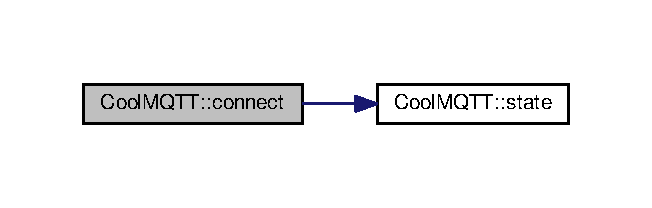
\includegraphics[width=313pt]{classCoolMQTT_a58b0b1f64b269c2681685208262fba1d_cgraph}
\end{center}
\end{figure}
Here is the caller graph for this function\+:
\nopagebreak
\begin{figure}[H]
\begin{center}
\leavevmode
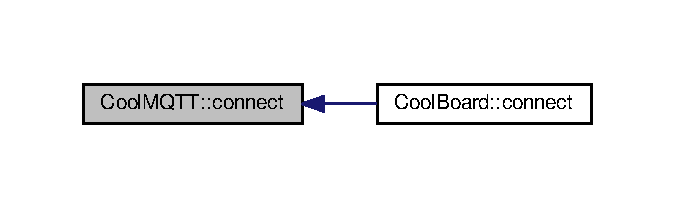
\includegraphics[width=350pt]{classCoolMQTT_a58b0b1f64b269c2681685208262fba1d_icgraph}
\end{center}
\end{figure}
\mbox{\Hypertarget{classCoolMQTT_a373cc92fca7760d886f02d8a6e5b3f63}\label{classCoolMQTT_a373cc92fca7760d886f02d8a6e5b3f63}} 
\index{Cool\+M\+Q\+TT@{Cool\+M\+Q\+TT}!get\+User@{get\+User}}
\index{get\+User@{get\+User}!Cool\+M\+Q\+TT@{Cool\+M\+Q\+TT}}
\subsubsection{\texorpdfstring{get\+User()}{getUser()}}
{\footnotesize\ttfamily String Cool\+M\+Q\+T\+T\+::get\+User (\begin{DoxyParamCaption}{ }\end{DoxyParamCaption})}

\hyperlink{classCoolMQTT_a373cc92fca7760d886f02d8a6e5b3f63}{Cool\+M\+Q\+T\+T\+::get\+User()}\+: This method is provided to get the user name 

Definition at line 659 of file Cool\+M\+Q\+T\+T.\+cpp.



References user.



Referenced by Cool\+Board\+::user\+Data().


\begin{DoxyCode}
660 \{
661 
662 \textcolor{preprocessor}{#if DEBUG == 1 }
663     Serial.println( F(\textcolor{stringliteral}{"Entering CoolMQTT.getUser()"}) );
664     Serial.println();
665     
666     Serial.print( F(\textcolor{stringliteral}{"user : "}) );
667     Serial.println(this->\hyperlink{classCoolMQTT_a8cd47e45d457f908d4b4390b35aaee83}{user});
668 
669 \textcolor{preprocessor}{#endif}
670 
671     \textcolor{keywordflow}{return} String(this->\hyperlink{classCoolMQTT_a8cd47e45d457f908d4b4390b35aaee83}{user});
672 \}
\end{DoxyCode}
Here is the caller graph for this function\+:
\nopagebreak
\begin{figure}[H]
\begin{center}
\leavevmode
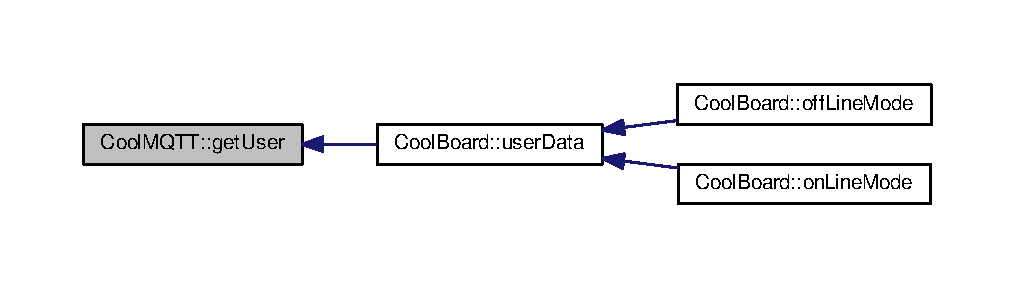
\includegraphics[width=350pt]{classCoolMQTT_a373cc92fca7760d886f02d8a6e5b3f63_icgraph}
\end{center}
\end{figure}
\mbox{\Hypertarget{classCoolMQTT_aa5eaae967b562b62cbcf2b8d81f6e5d5}\label{classCoolMQTT_aa5eaae967b562b62cbcf2b8d81f6e5d5}} 
\index{Cool\+M\+Q\+TT@{Cool\+M\+Q\+TT}!mqtt\+Loop@{mqtt\+Loop}}
\index{mqtt\+Loop@{mqtt\+Loop}!Cool\+M\+Q\+TT@{Cool\+M\+Q\+TT}}
\subsubsection{\texorpdfstring{mqtt\+Loop()}{mqttLoop()}}
{\footnotesize\ttfamily bool Cool\+M\+Q\+T\+T\+::mqtt\+Loop (\begin{DoxyParamCaption}{ }\end{DoxyParamCaption})}

\hyperlink{classCoolMQTT_aa5eaae967b562b62cbcf2b8d81f6e5d5}{Cool\+M\+Q\+T\+T\+::mqtt\+Loop()}\+: This method is provided to allow the client to process the data

\begin{DoxyReturn}{Returns}
true if successful,false otherwise 
\end{DoxyReturn}


Definition at line 244 of file Cool\+M\+Q\+T\+T.\+cpp.



References client.



Referenced by Cool\+Board\+::on\+Line\+Mode(), and Cool\+Board\+::update().


\begin{DoxyCode}
245 \{
246 
247     \textcolor{keywordtype}{unsigned} \textcolor{keywordtype}{long} lastTime=millis();
248 
249 \textcolor{preprocessor}{#if DEBUG == 1}
250 
251     Serial.println( F(\textcolor{stringliteral}{"Entering CoolMQTT.mqttLoop()"}) );
252     Serial.println();
253 
254 \textcolor{preprocessor}{#endif  }
255 
256     \textcolor{keywordflow}{while}( ( millis() - lastTime ) < 5000)
257     \{
258         this->\hyperlink{classCoolMQTT_a4ca71e4f76ef868692a297efd45b1415}{client}.loop();  
259     \}
260 
261 \textcolor{preprocessor}{#if DEBUG == 1 }
262     
263     Serial.print( F(\textcolor{stringliteral}{"loop result : "}) );
264     Serial.println( this->\hyperlink{classCoolMQTT_a4ca71e4f76ef868692a297efd45b1415}{client}.loop() );
265     Serial.println();
266 
267 \textcolor{preprocessor}{#endif}
268 
269     \textcolor{keywordflow}{return}( this->\hyperlink{classCoolMQTT_a4ca71e4f76ef868692a297efd45b1415}{client}.loop() );
270 \}
\end{DoxyCode}
Here is the caller graph for this function\+:
\nopagebreak
\begin{figure}[H]
\begin{center}
\leavevmode
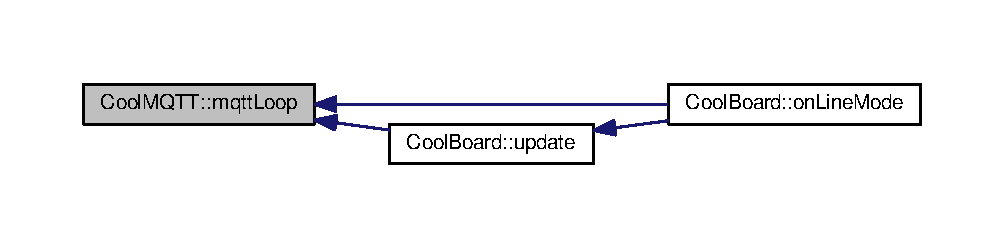
\includegraphics[width=350pt]{classCoolMQTT_aa5eaae967b562b62cbcf2b8d81f6e5d5_icgraph}
\end{center}
\end{figure}
\mbox{\Hypertarget{classCoolMQTT_a40553a0ad4b5ecf1cb4411ab54ca85fb}\label{classCoolMQTT_a40553a0ad4b5ecf1cb4411ab54ca85fb}} 
\index{Cool\+M\+Q\+TT@{Cool\+M\+Q\+TT}!print\+Conf@{print\+Conf}}
\index{print\+Conf@{print\+Conf}!Cool\+M\+Q\+TT@{Cool\+M\+Q\+TT}}
\subsubsection{\texorpdfstring{print\+Conf()}{printConf()}}
{\footnotesize\ttfamily void Cool\+M\+Q\+T\+T\+::print\+Conf (\begin{DoxyParamCaption}{ }\end{DoxyParamCaption})}

\hyperlink{classCoolMQTT_a40553a0ad4b5ecf1cb4411ab54ca85fb}{Cool\+M\+Q\+T\+T\+::print\+Conf()}\+: This method is provided to print the configuration to the Serial Monitor 

Definition at line 623 of file Cool\+M\+Q\+T\+T.\+cpp.



References buffer\+Size, in\+Topic, mqtt\+Server, out\+Topic, and user.



Referenced by Cool\+Board\+::begin().


\begin{DoxyCode}
624 \{
625 
626 \textcolor{preprocessor}{#if DEBUG == 1 }
627 
628     Serial.println( F(\textcolor{stringliteral}{"Entering CoolMQTT.printConf()"}) );
629     Serial.println();   
630 
631 \textcolor{preprocessor}{#endif}
632     
633     Serial.println(\textcolor{stringliteral}{"MQTT configuration "});
634 
635     Serial.print(\textcolor{stringliteral}{"mqttServer : "});
636     Serial.println(this->\hyperlink{classCoolMQTT_ab8bb951f87ddbf92db74c2ad16a3e53e}{mqttServer});
637 
638     Serial.print(\textcolor{stringliteral}{"inTopic : "});
639     Serial.println(this->\hyperlink{classCoolMQTT_a4492f52a441e83cc5151010317fdb52d}{inTopic});
640 
641     Serial.print(\textcolor{stringliteral}{"outTopic : "});
642     Serial.println(this->\hyperlink{classCoolMQTT_a109c786a17b463f9eeba046194279522}{outTopic});
643 
644     Serial.print(\textcolor{stringliteral}{"user : "});
645     Serial.println(this->\hyperlink{classCoolMQTT_a8cd47e45d457f908d4b4390b35aaee83}{user});
646 
647     Serial.print(\textcolor{stringliteral}{"bufferSize : "});
648     Serial.println(this->\hyperlink{classCoolMQTT_a7f3cf26b51d6770f216e42c5ef13ca9f}{bufferSize});
649 
650     Serial.println();
651 
652 
653 \}
\end{DoxyCode}
Here is the caller graph for this function\+:
\nopagebreak
\begin{figure}[H]
\begin{center}
\leavevmode
\includegraphics[width=318pt]{classCoolMQTT_a40553a0ad4b5ecf1cb4411ab54ca85fb_icgraph}
\end{center}
\end{figure}
\mbox{\Hypertarget{classCoolMQTT_ace977b3e90ab14b1199fe5c4fb0a13ec}\label{classCoolMQTT_ace977b3e90ab14b1199fe5c4fb0a13ec}} 
\index{Cool\+M\+Q\+TT@{Cool\+M\+Q\+TT}!publish@{publish}}
\index{publish@{publish}!Cool\+M\+Q\+TT@{Cool\+M\+Q\+TT}}
\subsubsection{\texorpdfstring{publish()}{publish()}\hspace{0.1cm}{\footnotesize\ttfamily [1/2]}}
{\footnotesize\ttfamily bool Cool\+M\+Q\+T\+T\+::publish (\begin{DoxyParamCaption}\item[{const char $\ast$}]{data }\end{DoxyParamCaption})}

Cool\+M\+Q\+T\+T\+::publish(data)\+: This method is provided to publish data to the out topic

\begin{DoxyReturn}{Returns}
true if publish successful, false otherwise 
\end{DoxyReturn}


Definition at line 152 of file Cool\+M\+Q\+T\+T.\+cpp.



References client, and out\+Topic.



Referenced by Cool\+Board\+::on\+Line\+Mode(), publish(), and Cool\+Board\+::update().


\begin{DoxyCode}
153 \{
154 
155 \textcolor{preprocessor}{#if DEBUG == 1 }
156 
157     Serial.println( F(\textcolor{stringliteral}{"Entering CoolMQTT.publish()"}) );
158     Serial.println();
159     \textcolor{comment}{//data is in JSON, publish it directly}
160 
161     Serial.println( F(\textcolor{stringliteral}{"data to publish : "}) );
162     Serial.println(data);
163     Serial.print( F(\textcolor{stringliteral}{"data size : "}) );
164     Serial.println(strlen(data));
165 
166     Serial.println();
167 
168 \textcolor{preprocessor}{#endif}
169     
170 
171     \textcolor{keywordtype}{bool} pub=\hyperlink{classCoolMQTT_a4ca71e4f76ef868692a297efd45b1415}{client}.publish( this->\hyperlink{classCoolMQTT_a109c786a17b463f9eeba046194279522}{outTopic},(byte*) data,strlen(data),\textcolor{keyword}{false}  );
172 
173 \textcolor{preprocessor}{#if DEBUG == 1 }
174 
175     Serial.print( F(\textcolor{stringliteral}{"success : "}) );
176     Serial.println(pub);    
177 
178 \textcolor{preprocessor}{#endif}
179 
180     \textcolor{keywordflow}{return}(pub);
181 
182 \}
\end{DoxyCode}
Here is the caller graph for this function\+:
\nopagebreak
\begin{figure}[H]
\begin{center}
\leavevmode
\includegraphics[width=350pt]{classCoolMQTT_ace977b3e90ab14b1199fe5c4fb0a13ec_icgraph}
\end{center}
\end{figure}
\mbox{\Hypertarget{classCoolMQTT_a65a506641740ce797ceadd4fa8a286d3}\label{classCoolMQTT_a65a506641740ce797ceadd4fa8a286d3}} 
\index{Cool\+M\+Q\+TT@{Cool\+M\+Q\+TT}!publish@{publish}}
\index{publish@{publish}!Cool\+M\+Q\+TT@{Cool\+M\+Q\+TT}}
\subsubsection{\texorpdfstring{publish()}{publish()}\hspace{0.1cm}{\footnotesize\ttfamily [2/2]}}
{\footnotesize\ttfamily bool Cool\+M\+Q\+T\+T\+::publish (\begin{DoxyParamCaption}\item[{const char $\ast$}]{data,  }\item[{int}]{log\+Interval }\end{DoxyParamCaption})}

Cool\+M\+Q\+T\+T\+::publish(data)\+: This method is provided to publish data to the out topic every log\+Interval ms

\begin{DoxyReturn}{Returns}
true if publish successful, false otherwise 
\end{DoxyReturn}


Definition at line 192 of file Cool\+M\+Q\+T\+T.\+cpp.



References previous\+Log\+Time, and publish().


\begin{DoxyCode}
193 \{
194 
195 \textcolor{preprocessor}{#if DEBUG == 1 }
196 
197     Serial.println( F(\textcolor{stringliteral}{"Entering CoolMQTT.publish() every logInterval "}) );
198     Serial.println();
199 
200 \textcolor{preprocessor}{#endif }
201     
202     \textcolor{keywordflow}{if}( ( millis() - ( this->\hyperlink{classCoolMQTT_a3db37ef9ed3b05b2a8d44edba0e7d3cc}{previousLogTime})  ) >=( logInterval ) )
203     \{
204     
205 \textcolor{preprocessor}{    #if DEBUG == 1}
206 
207         Serial.println( F(\textcolor{stringliteral}{"log Interval has passed "}) );
208         Serial.println();
209     
210 \textcolor{preprocessor}{    #endif}
211 
212         this->\hyperlink{classCoolMQTT_ace977b3e90ab14b1199fe5c4fb0a13ec}{publish}(data);
213 
214         this->\hyperlink{classCoolMQTT_a3db37ef9ed3b05b2a8d44edba0e7d3cc}{previousLogTime}=millis();
215     
216 \textcolor{preprocessor}{    #if DEBUG == 1 }
217 
218         Serial.print( F(\textcolor{stringliteral}{"last log time : "}) );
219         Serial.println(this->\hyperlink{classCoolMQTT_a3db37ef9ed3b05b2a8d44edba0e7d3cc}{previousLogTime});
220 
221 \textcolor{preprocessor}{    #endif}
222 
223         \textcolor{keywordflow}{return}(\textcolor{keyword}{true});
224     \}
225 
226 \textcolor{preprocessor}{#if DEBUG == 1 }
227 
228     Serial.println( F(\textcolor{stringliteral}{"log Interval still didn't pass "}) ); 
229     Serial.println();
230 
231 \textcolor{preprocessor}{#endif}
232 
233     \textcolor{keywordflow}{return}(\textcolor{keyword}{false});
234 \}
\end{DoxyCode}
Here is the call graph for this function\+:
\nopagebreak
\begin{figure}[H]
\begin{center}
\leavevmode
\includegraphics[width=318pt]{classCoolMQTT_a65a506641740ce797ceadd4fa8a286d3_cgraph}
\end{center}
\end{figure}
\mbox{\Hypertarget{classCoolMQTT_ae3c18f6ae9723746d32765f1c8f176ca}\label{classCoolMQTT_ae3c18f6ae9723746d32765f1c8f176ca}} 
\index{Cool\+M\+Q\+TT@{Cool\+M\+Q\+TT}!read@{read}}
\index{read@{read}!Cool\+M\+Q\+TT@{Cool\+M\+Q\+TT}}
\subsubsection{\texorpdfstring{read()}{read()}}
{\footnotesize\ttfamily String Cool\+M\+Q\+T\+T\+::read (\begin{DoxyParamCaption}{ }\end{DoxyParamCaption})}

\hyperlink{classCoolMQTT_ae3c18f6ae9723746d32765f1c8f176ca}{Cool\+M\+Q\+T\+T\+::read()}\+: This method is provided to return the last read message. 

Definition at line 358 of file Cool\+M\+Q\+T\+T.\+cpp.



References msg, and new\+Msg.



Referenced by Cool\+Board\+::on\+Line\+Mode().


\begin{DoxyCode}
359 \{   
360 
361 \textcolor{preprocessor}{#if DEBUG == 1 }
362 
363     Serial.println( F(\textcolor{stringliteral}{"Entering CoolMQTT.read()"}) );
364     Serial.println();
365 
366 \textcolor{preprocessor}{#endif }
367 
368     \textcolor{keywordflow}{if}(this->\hyperlink{classCoolMQTT_a3240388137b885775aadf38e96b24c6b}{newMsg}==\textcolor{keyword}{true})
369     \{
370         
371         this->\hyperlink{classCoolMQTT_a3240388137b885775aadf38e96b24c6b}{newMsg}=\textcolor{keyword}{false};
372 
373 \textcolor{preprocessor}{#if DEBUG == 1 }
374         Serial.println( F(\textcolor{stringliteral}{"received new message"}) );
375         Serial.println( F(\textcolor{stringliteral}{"message : "}) );
376         Serial.println(this->\hyperlink{classCoolMQTT_af6b19e7074dbbb4ae493c44dcb53f7ff}{msg});
377         Serial.println();
378 
379 \textcolor{preprocessor}{#endif}
380 
381         \textcolor{keywordflow}{return}(this->\hyperlink{classCoolMQTT_af6b19e7074dbbb4ae493c44dcb53f7ff}{msg});
382         
383     \}
384     \textcolor{keywordflow}{return}(\textcolor{stringliteral}{""});
385 
386 \}
\end{DoxyCode}
Here is the caller graph for this function\+:
\nopagebreak
\begin{figure}[H]
\begin{center}
\leavevmode
\includegraphics[width=326pt]{classCoolMQTT_ae3c18f6ae9723746d32765f1c8f176ca_icgraph}
\end{center}
\end{figure}
\mbox{\Hypertarget{classCoolMQTT_a5d003307eff78efbd585e42b43b72b6d}\label{classCoolMQTT_a5d003307eff78efbd585e42b43b72b6d}} 
\index{Cool\+M\+Q\+TT@{Cool\+M\+Q\+TT}!state@{state}}
\index{state@{state}!Cool\+M\+Q\+TT@{Cool\+M\+Q\+TT}}
\subsubsection{\texorpdfstring{state()}{state()}}
{\footnotesize\ttfamily int Cool\+M\+Q\+T\+T\+::state (\begin{DoxyParamCaption}{ }\end{DoxyParamCaption})}

\hyperlink{classCoolMQTT_a5d003307eff78efbd585e42b43b72b6d}{Cool\+M\+Q\+T\+T\+::state()}\+: This method is provided to return the mqtt client\textquotesingle{}s state. \begin{DoxyReturn}{Returns}
mqtt client state\+: -\/4 \+: M\+Q\+T\+T\+\_\+\+C\+O\+N\+N\+E\+C\+T\+I\+O\+N\+\_\+\+T\+I\+M\+E\+O\+UT -\/ the server didn\textquotesingle{}t respond within the keepalive time -\/3 \+: M\+Q\+T\+T\+\_\+\+C\+O\+N\+N\+E\+C\+T\+I\+O\+N\+\_\+\+L\+O\+ST -\/ the network connection was broken -\/2 \+: M\+Q\+T\+T\+\_\+\+C\+O\+N\+N\+E\+C\+T\+\_\+\+F\+A\+I\+L\+ED -\/ the network connection failed -\/1 \+: M\+Q\+T\+T\+\_\+\+D\+I\+S\+C\+O\+N\+N\+E\+C\+T\+ED -\/ the client is disconnected cleanly 0 \+: M\+Q\+T\+T\+\_\+\+C\+O\+N\+N\+E\+C\+T\+ED -\/ the cient is connected 1 \+: M\+Q\+T\+T\+\_\+\+C\+O\+N\+N\+E\+C\+T\+\_\+\+B\+A\+D\+\_\+\+P\+R\+O\+T\+O\+C\+OL -\/ the server doesn\textquotesingle{}t support the requested version of M\+Q\+TT 2 \+: M\+Q\+T\+T\+\_\+\+C\+O\+N\+N\+E\+C\+T\+\_\+\+B\+A\+D\+\_\+\+C\+L\+I\+E\+N\+T\+\_\+\+ID -\/ the server rejected the client identifier 3 \+: M\+Q\+T\+T\+\_\+\+C\+O\+N\+N\+E\+C\+T\+\_\+\+U\+N\+A\+V\+A\+I\+L\+A\+B\+LE -\/ the server was unable to accept the connection 4 \+: M\+Q\+T\+T\+\_\+\+C\+O\+N\+N\+E\+C\+T\+\_\+\+B\+A\+D\+\_\+\+C\+R\+E\+D\+E\+N\+T\+I\+A\+LS -\/ the username/password were rejected 5 \+: M\+Q\+T\+T\+\_\+\+C\+O\+N\+N\+E\+C\+T\+\_\+\+U\+N\+A\+U\+T\+H\+O\+R\+I\+Z\+ED -\/ the client was not authorized to connect 
\end{DoxyReturn}


Definition at line 72 of file Cool\+M\+Q\+T\+T.\+cpp.



References client.



Referenced by connect(), and Cool\+Board\+::connect().


\begin{DoxyCode}
73 \{
74 
75 \textcolor{preprocessor}{#if DEBUG == 1 }
76 
77     Serial.println( F(\textcolor{stringliteral}{"Entering CoolMQTT.state()"}) );
78     Serial.println();   
79     Serial.print( F(\textcolor{stringliteral}{"state : "}) );
80     Serial.println( this->\hyperlink{classCoolMQTT_a4ca71e4f76ef868692a297efd45b1415}{client}.state() );
81 
82 \textcolor{preprocessor}{#endif}
83     
84     \textcolor{keywordflow}{return}( this->\hyperlink{classCoolMQTT_a4ca71e4f76ef868692a297efd45b1415}{client}.state() );
85 \}
\end{DoxyCode}
Here is the caller graph for this function\+:
\nopagebreak
\begin{figure}[H]
\begin{center}
\leavevmode
\includegraphics[width=350pt]{classCoolMQTT_a5d003307eff78efbd585e42b43b72b6d_icgraph}
\end{center}
\end{figure}


\subsection{Member Data Documentation}
\mbox{\Hypertarget{classCoolMQTT_a7f3cf26b51d6770f216e42c5ef13ca9f}\label{classCoolMQTT_a7f3cf26b51d6770f216e42c5ef13ca9f}} 
\index{Cool\+M\+Q\+TT@{Cool\+M\+Q\+TT}!buffer\+Size@{buffer\+Size}}
\index{buffer\+Size@{buffer\+Size}!Cool\+M\+Q\+TT@{Cool\+M\+Q\+TT}}
\subsubsection{\texorpdfstring{buffer\+Size}{bufferSize}}
{\footnotesize\ttfamily int Cool\+M\+Q\+T\+T\+::buffer\+Size =3000\hspace{0.3cm}{\ttfamily [private]}}



Definition at line 63 of file Cool\+M\+Q\+T\+T.\+h.



Referenced by begin(), config(), and print\+Conf().

\mbox{\Hypertarget{classCoolMQTT_a4ca71e4f76ef868692a297efd45b1415}\label{classCoolMQTT_a4ca71e4f76ef868692a297efd45b1415}} 
\index{Cool\+M\+Q\+TT@{Cool\+M\+Q\+TT}!client@{client}}
\index{client@{client}!Cool\+M\+Q\+TT@{Cool\+M\+Q\+TT}}
\subsubsection{\texorpdfstring{client}{client}}
{\footnotesize\ttfamily Pub\+Sub\+Client Cool\+M\+Q\+T\+T\+::client\hspace{0.3cm}{\ttfamily [private]}}



Definition at line 67 of file Cool\+M\+Q\+T\+T.\+h.



Referenced by begin(), connect(), mqtt\+Loop(), publish(), and state().

\mbox{\Hypertarget{classCoolMQTT_acc30a0200967374a524092a8a806502a}\label{classCoolMQTT_acc30a0200967374a524092a8a806502a}} 
\index{Cool\+M\+Q\+TT@{Cool\+M\+Q\+TT}!esp\+Client@{esp\+Client}}
\index{esp\+Client@{esp\+Client}!Cool\+M\+Q\+TT@{Cool\+M\+Q\+TT}}
\subsubsection{\texorpdfstring{esp\+Client}{espClient}}
{\footnotesize\ttfamily Wi\+Fi\+Client Cool\+M\+Q\+T\+T\+::esp\+Client\hspace{0.3cm}{\ttfamily [private]}}



Definition at line 65 of file Cool\+M\+Q\+T\+T.\+h.



Referenced by begin().

\mbox{\Hypertarget{classCoolMQTT_a4492f52a441e83cc5151010317fdb52d}\label{classCoolMQTT_a4492f52a441e83cc5151010317fdb52d}} 
\index{Cool\+M\+Q\+TT@{Cool\+M\+Q\+TT}!in\+Topic@{in\+Topic}}
\index{in\+Topic@{in\+Topic}!Cool\+M\+Q\+TT@{Cool\+M\+Q\+TT}}
\subsubsection{\texorpdfstring{in\+Topic}{inTopic}}
{\footnotesize\ttfamily char Cool\+M\+Q\+T\+T\+::in\+Topic\mbox{[}50\mbox{]} =\{\textquotesingle{}0\textquotesingle{}\}\hspace{0.3cm}{\ttfamily [private]}}



Definition at line 57 of file Cool\+M\+Q\+T\+T.\+h.



Referenced by config(), connect(), and print\+Conf().

\mbox{\Hypertarget{classCoolMQTT_ab8bb951f87ddbf92db74c2ad16a3e53e}\label{classCoolMQTT_ab8bb951f87ddbf92db74c2ad16a3e53e}} 
\index{Cool\+M\+Q\+TT@{Cool\+M\+Q\+TT}!mqtt\+Server@{mqtt\+Server}}
\index{mqtt\+Server@{mqtt\+Server}!Cool\+M\+Q\+TT@{Cool\+M\+Q\+TT}}
\subsubsection{\texorpdfstring{mqtt\+Server}{mqttServer}}
{\footnotesize\ttfamily char Cool\+M\+Q\+T\+T\+::mqtt\+Server\mbox{[}50\mbox{]} =\{\textquotesingle{}0\textquotesingle{}\}\hspace{0.3cm}{\ttfamily [private]}}



Definition at line 53 of file Cool\+M\+Q\+T\+T.\+h.



Referenced by begin(), config(), and print\+Conf().

\mbox{\Hypertarget{classCoolMQTT_af6b19e7074dbbb4ae493c44dcb53f7ff}\label{classCoolMQTT_af6b19e7074dbbb4ae493c44dcb53f7ff}} 
\index{Cool\+M\+Q\+TT@{Cool\+M\+Q\+TT}!msg@{msg}}
\index{msg@{msg}!Cool\+M\+Q\+TT@{Cool\+M\+Q\+TT}}
\subsubsection{\texorpdfstring{msg}{msg}}
{\footnotesize\ttfamily String Cool\+M\+Q\+T\+T\+::msg =\char`\"{}\char`\"{}\hspace{0.3cm}{\ttfamily [private]}}



Definition at line 55 of file Cool\+M\+Q\+T\+T.\+h.



Referenced by callback(), and read().

\mbox{\Hypertarget{classCoolMQTT_a3240388137b885775aadf38e96b24c6b}\label{classCoolMQTT_a3240388137b885775aadf38e96b24c6b}} 
\index{Cool\+M\+Q\+TT@{Cool\+M\+Q\+TT}!new\+Msg@{new\+Msg}}
\index{new\+Msg@{new\+Msg}!Cool\+M\+Q\+TT@{Cool\+M\+Q\+TT}}
\subsubsection{\texorpdfstring{new\+Msg}{newMsg}}
{\footnotesize\ttfamily bool Cool\+M\+Q\+T\+T\+::new\+Msg =0\hspace{0.3cm}{\ttfamily [private]}}



Definition at line 69 of file Cool\+M\+Q\+T\+T.\+h.



Referenced by callback(), and read().

\mbox{\Hypertarget{classCoolMQTT_a109c786a17b463f9eeba046194279522}\label{classCoolMQTT_a109c786a17b463f9eeba046194279522}} 
\index{Cool\+M\+Q\+TT@{Cool\+M\+Q\+TT}!out\+Topic@{out\+Topic}}
\index{out\+Topic@{out\+Topic}!Cool\+M\+Q\+TT@{Cool\+M\+Q\+TT}}
\subsubsection{\texorpdfstring{out\+Topic}{outTopic}}
{\footnotesize\ttfamily char Cool\+M\+Q\+T\+T\+::out\+Topic\mbox{[}50\mbox{]} =\{\textquotesingle{}0\textquotesingle{}\}\hspace{0.3cm}{\ttfamily [private]}}



Definition at line 59 of file Cool\+M\+Q\+T\+T.\+h.



Referenced by config(), print\+Conf(), and publish().

\mbox{\Hypertarget{classCoolMQTT_a3db37ef9ed3b05b2a8d44edba0e7d3cc}\label{classCoolMQTT_a3db37ef9ed3b05b2a8d44edba0e7d3cc}} 
\index{Cool\+M\+Q\+TT@{Cool\+M\+Q\+TT}!previous\+Log\+Time@{previous\+Log\+Time}}
\index{previous\+Log\+Time@{previous\+Log\+Time}!Cool\+M\+Q\+TT@{Cool\+M\+Q\+TT}}
\subsubsection{\texorpdfstring{previous\+Log\+Time}{previousLogTime}}
{\footnotesize\ttfamily unsigned long Cool\+M\+Q\+T\+T\+::previous\+Log\+Time =0\hspace{0.3cm}{\ttfamily [private]}}



Definition at line 71 of file Cool\+M\+Q\+T\+T.\+h.



Referenced by publish().

\mbox{\Hypertarget{classCoolMQTT_a8cd47e45d457f908d4b4390b35aaee83}\label{classCoolMQTT_a8cd47e45d457f908d4b4390b35aaee83}} 
\index{Cool\+M\+Q\+TT@{Cool\+M\+Q\+TT}!user@{user}}
\index{user@{user}!Cool\+M\+Q\+TT@{Cool\+M\+Q\+TT}}
\subsubsection{\texorpdfstring{user}{user}}
{\footnotesize\ttfamily char Cool\+M\+Q\+T\+T\+::user\mbox{[}50\mbox{]} =\{\textquotesingle{}0\textquotesingle{}\}\hspace{0.3cm}{\ttfamily [private]}}



Definition at line 61 of file Cool\+M\+Q\+T\+T.\+h.



Referenced by config(), connect(), get\+User(), and print\+Conf().



The documentation for this class was generated from the following files\+:\begin{DoxyCompactItemize}
\item 
/home/ashiroji/\+Arduino/libraries/\+Cool\+Board/\hyperlink{CoolMQTT_8h}{Cool\+M\+Q\+T\+T.\+h}\item 
/home/ashiroji/\+Arduino/libraries/\+Cool\+Board/\hyperlink{CoolMQTT_8cpp}{Cool\+M\+Q\+T\+T.\+cpp}\end{DoxyCompactItemize}

\hypertarget{classCoolTime}{}\section{Cool\+Time Class Reference}
\label{classCoolTime}\index{Cool\+Time@{Cool\+Time}}


This class manages the D\+S1337 R\+TC .  




{\ttfamily \#include $<$Cool\+Time.\+h$>$}



Collaboration diagram for Cool\+Time\+:\nopagebreak
\begin{figure}[H]
\begin{center}
\leavevmode
\includegraphics[width=188pt]{classCoolTime__coll__graph}
\end{center}
\end{figure}
\subsection*{Public Member Functions}
\begin{DoxyCompactItemize}
\item 
void \hyperlink{classCoolTime_ab1976cf718b950bc31e003c3323b8adb}{begin} ()
\item 
void \hyperlink{classCoolTime_aae601f795452cfa48d9fb337aed483a8}{update} ()
\item 
bool \hyperlink{classCoolTime_a87c28260c1bc77091162cbcf1ee2e129}{config} ()
\item 
void \hyperlink{classCoolTime_a014656d0d3f74d6391364b92b13e0780}{config} (I\+P\+Address \hyperlink{classCoolTime_ad2b9858f399108cb440dd1e908916f04}{time\+Server}, unsigned int \hyperlink{classCoolTime_a2f777da44d7ba678be8185299e9b49d1}{local\+Port})
\item 
void \hyperlink{classCoolTime_af355e7f9b3898211cd2ff25eab5933b1}{print\+Conf} ()
\item 
void \hyperlink{classCoolTime_ab81ea7fdaace111aa01cc1ec84c6d297}{set\+Date\+Time} (int year, int month, int day, int hour, int minutes, int seconds)
\item 
tm\+Elements\+\_\+t \hyperlink{classCoolTime_a7a7501c5ca77dd1248bea704c44f986c}{get\+Time\+Date} ()
\item 
String \hyperlink{classCoolTime_ac4f32ee513c1328d984306645e8785a4}{get\+E\+S\+Date} ()
\item 
unsigned long \hyperlink{classCoolTime_a5d17f707a9d337720493b2bce9d41c21}{get\+Last\+Sync\+Time} ()
\item 
bool \hyperlink{classCoolTime_a5ae038a4498602b189f76a10bf02adf8}{is\+Time\+Sync} (unsigned long seconds=604800)
\item 
time\+\_\+t \hyperlink{classCoolTime_a41fbbbfd651c2079f54d4b2911e4c705}{get\+Ntp\+Time} ()
\item 
void \hyperlink{classCoolTime_a236a38d120dc53bc67456d763838c5a1}{send\+N\+T\+Ppacket} (I\+P\+Address \&address)
\item 
String \hyperlink{classCoolTime_acd537cd4210d7bde4e1f5c47d2ac0456}{format\+Digits} (int digits)
\item 
bool \hyperlink{classCoolTime_ae9658c9b377510d469e3b88edf33ee85}{save\+Time\+Sync} ()
\end{DoxyCompactItemize}
\subsection*{Private Attributes}
\begin{DoxyCompactItemize}
\item 
unsigned long \hyperlink{classCoolTime_a9d032e76c3470a15b3bbbc52af6463f7}{time\+Sync} =0
\item 
I\+P\+Address \hyperlink{classCoolTime_ad2b9858f399108cb440dd1e908916f04}{time\+Server}
\item 
Wi\+Fi\+U\+DP \hyperlink{classCoolTime_a4e23216a8121ca79d0fb019f30884b92}{Udp}
\item 
unsigned int \hyperlink{classCoolTime_a2f777da44d7ba678be8185299e9b49d1}{local\+Port} =0
\item 
byte \hyperlink{classCoolTime_a27e6abc82a5c2f72161956967005bec7}{packet\+Buffer} \mbox{[}\hyperlink{CoolTime_8h_a56a6ea64006651b4f42adf713e244f06}{N\+T\+P\+\_\+\+P\+A\+C\+K\+E\+T\+\_\+\+S\+I\+ZE}\mbox{]}
\item 
tm\+Elements\+\_\+t \hyperlink{classCoolTime_ad33c2713c903ff064ad09c46406ae088}{tm\+Set}
\item 
D\+S1337\+R\+TC \hyperlink{classCoolTime_abd38f2384ff90692b1568d9db869412e}{rtc}
\end{DoxyCompactItemize}


\subsection{Detailed Description}
This class manages the D\+S1337 R\+TC . 

Definition at line 31 of file Cool\+Time.\+h.



\subsection{Member Function Documentation}
\mbox{\Hypertarget{classCoolTime_ab1976cf718b950bc31e003c3323b8adb}\label{classCoolTime_ab1976cf718b950bc31e003c3323b8adb}} 
\index{Cool\+Time@{Cool\+Time}!begin@{begin}}
\index{begin@{begin}!Cool\+Time@{Cool\+Time}}
\subsubsection{\texorpdfstring{begin()}{begin()}}
{\footnotesize\ttfamily void Cool\+Time\+::begin (\begin{DoxyParamCaption}{ }\end{DoxyParamCaption})}

\hyperlink{classCoolTime_ab1976cf718b950bc31e003c3323b8adb}{Cool\+Time\+::begin()}\+: This method is provided to init the udp connection 

Definition at line 41 of file Cool\+Time.\+cpp.



References local\+Port, Udp, and update().



Referenced by Cool\+Board\+::begin().


\begin{DoxyCode}
42 \{
43 
44 \textcolor{preprocessor}{#if DEBUG == 1 }
45 
46     Serial.println( F(\textcolor{stringliteral}{"Entering CoolTime.begin()"}) );
47     Serial.println();
48 
49 \textcolor{preprocessor}{#endif }
50 
51 
52     \hyperlink{classCoolTime_a4e23216a8121ca79d0fb019f30884b92}{Udp}.begin(\hyperlink{classCoolTime_a2f777da44d7ba678be8185299e9b49d1}{localPort});
53     
54     this->\hyperlink{classCoolTime_aae601f795452cfa48d9fb337aed483a8}{update}();
55     
56 \}
\end{DoxyCode}
Here is the call graph for this function\+:\nopagebreak
\begin{figure}[H]
\begin{center}
\leavevmode
\includegraphics[width=350pt]{classCoolTime_ab1976cf718b950bc31e003c3323b8adb_cgraph}
\end{center}
\end{figure}
Here is the caller graph for this function\+:\nopagebreak
\begin{figure}[H]
\begin{center}
\leavevmode
\includegraphics[width=296pt]{classCoolTime_ab1976cf718b950bc31e003c3323b8adb_icgraph}
\end{center}
\end{figure}
\mbox{\Hypertarget{classCoolTime_a87c28260c1bc77091162cbcf1ee2e129}\label{classCoolTime_a87c28260c1bc77091162cbcf1ee2e129}} 
\index{Cool\+Time@{Cool\+Time}!config@{config}}
\index{config@{config}!Cool\+Time@{Cool\+Time}}
\subsubsection{\texorpdfstring{config()}{config()}\hspace{0.1cm}{\footnotesize\ttfamily [1/2]}}
{\footnotesize\ttfamily bool Cool\+Time\+::config (\begin{DoxyParamCaption}{ }\end{DoxyParamCaption})}

\hyperlink{classCoolTime_a87c28260c1bc77091162cbcf1ee2e129}{Cool\+Time\+::config()}\+: This method is provided to configure the \hyperlink{classCoolTime}{Cool\+Time} object through a configuration file.

\begin{DoxyReturn}{Returns}
true if successful,false otherwise 
\end{DoxyReturn}


Definition at line 424 of file Cool\+Time.\+cpp.



References local\+Port, time\+Server, and time\+Sync.



Referenced by Cool\+Board\+::begin(), and Cool\+Board\+::update().


\begin{DoxyCode}
425 \{
426 
427 \textcolor{preprocessor}{#if DEBUG == 1 }
428 
429     Serial.println( F(\textcolor{stringliteral}{"Enter CoolTime.config()"}) );
430     Serial.println();
431 
432 \textcolor{preprocessor}{#endif }
433 
434     File rtcConfig = SPIFFS.open(\textcolor{stringliteral}{"/rtcConfig.json"}, \textcolor{stringliteral}{"r"});
435 
436     \textcolor{keywordflow}{if} (!rtcConfig) 
437     \{
438     
439 \textcolor{preprocessor}{    #if DEBUG == 1 }
440 
441         Serial.println( F(\textcolor{stringliteral}{"failed to read /rtcConfig.json"}) );
442         Serial.println();
443     
444 \textcolor{preprocessor}{    #endif}
445 
446         \textcolor{keywordflow}{return}(\textcolor{keyword}{false});
447     \}
448     \textcolor{keywordflow}{else}
449     \{
450         \textcolor{keywordtype}{size\_t} size = rtcConfig.size();
451         \textcolor{comment}{// Allocate a buffer to store contents of the file.}
452         std::unique\_ptr<char[]> buf(\textcolor{keyword}{new} \textcolor{keywordtype}{char}[size]);
453 
454         rtcConfig.readBytes(buf.get(), size);
455         DynamicJsonBuffer jsonBuffer;
456         JsonObject& json = jsonBuffer.parseObject(buf.get());
457         \textcolor{keywordflow}{if} (!json.success()) 
458         \{
459         
460 \textcolor{preprocessor}{        #if DEBUG == 1 }
461 
462             Serial.println( F(\textcolor{stringliteral}{"failed to parse json"}) );
463             Serial.println();
464         
465 \textcolor{preprocessor}{        #endif }
466 
467             \textcolor{keywordflow}{return}(\textcolor{keyword}{false});
468         \} 
469         \textcolor{keywordflow}{else}
470         \{  
471         
472 \textcolor{preprocessor}{        #if DEBUG == 1 }
473 
474             Serial.println( F(\textcolor{stringliteral}{"configuration json is :"}) );
475             json.printTo(Serial);
476             Serial.println();
477 
478 \textcolor{preprocessor}{        #endif}
479 
480             String ip;
481             
482             \textcolor{keywordflow}{if}(json[\textcolor{stringliteral}{"timeServer"}].success() )
483             \{           
484                  ip=json[\textcolor{stringliteral}{"timeServer"}].as<String>();
485                 this->\hyperlink{classCoolTime_ad2b9858f399108cb440dd1e908916f04}{timeServer}.fromString(ip);
486                 
487             \}
488             \textcolor{keywordflow}{else}
489             \{
490                 this->\hyperlink{classCoolTime_ad2b9858f399108cb440dd1e908916f04}{timeServer}=this->\hyperlink{classCoolTime_ad2b9858f399108cb440dd1e908916f04}{timeServer};
491             \}
492             json[\textcolor{stringliteral}{"timeServer"}]=ip;
493             
494             \textcolor{keywordflow}{if}(json[\textcolor{stringliteral}{"localPort"}].success() )
495             \{                       
496                 this->\hyperlink{classCoolTime_a2f777da44d7ba678be8185299e9b49d1}{localPort}=json[\textcolor{stringliteral}{"localPort"}];
497             \}
498             \textcolor{keywordflow}{else}
499             \{
500                 this->\hyperlink{classCoolTime_a2f777da44d7ba678be8185299e9b49d1}{localPort}=this->\hyperlink{classCoolTime_a2f777da44d7ba678be8185299e9b49d1}{localPort};
501             \}
502             json[\textcolor{stringliteral}{"localPort"}]=this->\hyperlink{classCoolTime_a2f777da44d7ba678be8185299e9b49d1}{localPort};
503 
504 
505             \textcolor{keywordflow}{if}( json[\textcolor{stringliteral}{"timeSync"}].success() )
506             \{
507 
508                 this->\hyperlink{classCoolTime_a9d032e76c3470a15b3bbbc52af6463f7}{timeSync}=json[\textcolor{stringliteral}{"timeSync"}];
509             \}
510             \textcolor{keywordflow}{else}
511             \{
512                 this->\hyperlink{classCoolTime_a9d032e76c3470a15b3bbbc52af6463f7}{timeSync}=this->\hyperlink{classCoolTime_a9d032e76c3470a15b3bbbc52af6463f7}{timeSync};
513             \}
514             json[\textcolor{stringliteral}{"timeSync"}]=this->\hyperlink{classCoolTime_a9d032e76c3470a15b3bbbc52af6463f7}{timeSync};
515 
516             rtcConfig.close();
517             rtcConfig= SPIFFS.open(\textcolor{stringliteral}{"/rtcConfig.json"}, \textcolor{stringliteral}{"w"});
518             
519             \textcolor{keywordflow}{if}(!rtcConfig)
520             \{
521             
522 \textcolor{preprocessor}{            #if DEBUG == 1}
523 
524                 Serial.println( F(\textcolor{stringliteral}{"failed to write to /rtcConfig.json"}) );
525                 Serial.println();
526             
527 \textcolor{preprocessor}{            #endif}
528 
529                 \textcolor{keywordflow}{return}(\textcolor{keyword}{false});
530             \}
531             
532             json.printTo(rtcConfig);
533             rtcConfig.close();
534 
535 \textcolor{preprocessor}{        #if DEBUG == 1 }
536 
537             Serial.println( F(\textcolor{stringliteral}{"configuration is :"}) );
538             json.printTo(Serial);
539             Serial.println();
540         
541 \textcolor{preprocessor}{        #endif}
542         
543             \textcolor{keywordflow}{return}(\textcolor{keyword}{true}); 
544         \}
545     \}   
546 
547 
548 
549 \}
\end{DoxyCode}
Here is the caller graph for this function\+:\nopagebreak
\begin{figure}[H]
\begin{center}
\leavevmode
\includegraphics[width=350pt]{classCoolTime_a87c28260c1bc77091162cbcf1ee2e129_icgraph}
\end{center}
\end{figure}
\mbox{\Hypertarget{classCoolTime_a014656d0d3f74d6391364b92b13e0780}\label{classCoolTime_a014656d0d3f74d6391364b92b13e0780}} 
\index{Cool\+Time@{Cool\+Time}!config@{config}}
\index{config@{config}!Cool\+Time@{Cool\+Time}}
\subsubsection{\texorpdfstring{config()}{config()}\hspace{0.1cm}{\footnotesize\ttfamily [2/2]}}
{\footnotesize\ttfamily void Cool\+Time\+::config (\begin{DoxyParamCaption}\item[{I\+P\+Address}]{time\+Server,  }\item[{unsigned int}]{local\+Port }\end{DoxyParamCaption})}

Cool\+Time\+::config(\+Time server I\+P , udp Port)\+: This method is provided to do manual configuration. 

Definition at line 401 of file Cool\+Time.\+cpp.



References local\+Port, and time\+Server.


\begin{DoxyCode}
402 \{
403 
404 \textcolor{preprocessor}{#if DEBUG == 1 }
405 
406     Serial.println( F(\textcolor{stringliteral}{"Enter CoomTime.config() , no SPIFFS variant "}) );
407     Serial.println();
408 
409 \textcolor{preprocessor}{#endif }
410 
411     this->\hyperlink{classCoolTime_ad2b9858f399108cb440dd1e908916f04}{timeServer}=\hyperlink{classCoolTime_ad2b9858f399108cb440dd1e908916f04}{timeServer};
412     this->\hyperlink{classCoolTime_a2f777da44d7ba678be8185299e9b49d1}{localPort}=\hyperlink{classCoolTime_a2f777da44d7ba678be8185299e9b49d1}{localPort};
413     
414 \} 
\end{DoxyCode}
\mbox{\Hypertarget{classCoolTime_acd537cd4210d7bde4e1f5c47d2ac0456}\label{classCoolTime_acd537cd4210d7bde4e1f5c47d2ac0456}} 
\index{Cool\+Time@{Cool\+Time}!format\+Digits@{format\+Digits}}
\index{format\+Digits@{format\+Digits}!Cool\+Time@{Cool\+Time}}
\subsubsection{\texorpdfstring{format\+Digits()}{formatDigits()}}
{\footnotesize\ttfamily String Cool\+Time\+::format\+Digits (\begin{DoxyParamCaption}\item[{int}]{digits }\end{DoxyParamCaption})}

Cool\+Time\+::print\+Digits(digit)

utility method for digital clock display adds leading 0

\begin{DoxyReturn}{Returns}
formatted string of the input digit 
\end{DoxyReturn}


Definition at line 691 of file Cool\+Time.\+cpp.



Referenced by get\+E\+S\+Date(), get\+Time\+Date(), and set\+Date\+Time().


\begin{DoxyCode}
692 \{
693 
694 \textcolor{preprocessor}{#if DEBUG == 1 }
695 
696     Serial.println( F(\textcolor{stringliteral}{"Entering CoolTime.formatDigits()"}) );
697     Serial.println();
698 
699 \textcolor{preprocessor}{#endif }
700 
701     \textcolor{keywordflow}{if}(digits < 10)
702     \{
703     
704 \textcolor{preprocessor}{    #if DEBUG == 1}
705 
706         Serial.println( F(\textcolor{stringliteral}{"output digit : "}) );
707         Serial.println( String(\textcolor{stringliteral}{"0"}) + String(digits) );
708 
709 \textcolor{preprocessor}{    #endif}
710 
711         \textcolor{keywordflow}{return}( String(\textcolor{stringliteral}{"0"}) + String(digits) );
712     \}
713     
714 \textcolor{preprocessor}{#if DEBUG == 1 }
715 
716     Serial.println( F(\textcolor{stringliteral}{"output digit : "}) );
717     Serial.println(digits);
718 
719 \textcolor{preprocessor}{#endif}
720 
721     \textcolor{keywordflow}{return}( String(digits) );
722 \}
\end{DoxyCode}
Here is the caller graph for this function\+:
\nopagebreak
\begin{figure}[H]
\begin{center}
\leavevmode
\includegraphics[width=350pt]{classCoolTime_acd537cd4210d7bde4e1f5c47d2ac0456_icgraph}
\end{center}
\end{figure}
\mbox{\Hypertarget{classCoolTime_ac4f32ee513c1328d984306645e8785a4}\label{classCoolTime_ac4f32ee513c1328d984306645e8785a4}} 
\index{Cool\+Time@{Cool\+Time}!get\+E\+S\+Date@{get\+E\+S\+Date}}
\index{get\+E\+S\+Date@{get\+E\+S\+Date}!Cool\+Time@{Cool\+Time}}
\subsubsection{\texorpdfstring{get\+E\+S\+Date()}{getESDate()}}
{\footnotesize\ttfamily String Cool\+Time\+::get\+E\+S\+Date (\begin{DoxyParamCaption}{ }\end{DoxyParamCaption})}

Cool\+Time\+::get\+E\+S\+D()\+: This method is provided to return an Elastic Search compatible date Format

\begin{DoxyReturn}{Returns}
date String in Elastic Search format 
\end{DoxyReturn}


Definition at line 193 of file Cool\+Time.\+cpp.



References format\+Digits(), and get\+Time\+Date().



Referenced by set\+Date\+Time(), and Cool\+Board\+::user\+Data().


\begin{DoxyCode}
194 \{
195 
196 \textcolor{preprocessor}{#if DEBUG == 1 }
197 
198     Serial.println( F(\textcolor{stringliteral}{"Entering CoolTime.getESDate()"}) );
199     Serial.println();
200 
201 \textcolor{preprocessor}{#endif }
202 
203     tmElements\_t tm=this->\hyperlink{classCoolTime_a7a7501c5ca77dd1248bea704c44f986c}{getTimeDate}();
204 
205     \textcolor{comment}{//"20yy-mm-ddT00:00:00Z"}
206     String elasticSearchString =String(tm.Year+1970)+\textcolor{stringliteral}{"-"}+this->\hyperlink{classCoolTime_acd537cd4210d7bde4e1f5c47d2ac0456}{formatDigits}(tm.Month)+\textcolor{stringliteral}{"-"};
207 
208     elasticSearchString +=this->\hyperlink{classCoolTime_acd537cd4210d7bde4e1f5c47d2ac0456}{formatDigits}(tm.Day)+\textcolor{stringliteral}{"T"}+this->
      \hyperlink{classCoolTime_acd537cd4210d7bde4e1f5c47d2ac0456}{formatDigits}(tm.Hour)+\textcolor{stringliteral}{":"};
209     
210     elasticSearchString +=this->\hyperlink{classCoolTime_acd537cd4210d7bde4e1f5c47d2ac0456}{formatDigits}(tm.Minute)+\textcolor{stringliteral}{":"}+this->
      \hyperlink{classCoolTime_acd537cd4210d7bde4e1f5c47d2ac0456}{formatDigits}(tm.Second)+\textcolor{stringliteral}{"Z"};
211 
212 \textcolor{preprocessor}{#if DEBUG == 1 }
213 
214     Serial.print( F(\textcolor{stringliteral}{"elastic Search date : "}) );
215     Serial.println(elasticSearchString);
216     Serial.println();
217 
218 \textcolor{preprocessor}{#endif}
219 
220     \textcolor{keywordflow}{return} (elasticSearchString);
221 \}
\end{DoxyCode}
Here is the call graph for this function\+:
\nopagebreak
\begin{figure}[H]
\begin{center}
\leavevmode
\includegraphics[width=350pt]{classCoolTime_ac4f32ee513c1328d984306645e8785a4_cgraph}
\end{center}
\end{figure}
Here is the caller graph for this function\+:
\nopagebreak
\begin{figure}[H]
\begin{center}
\leavevmode
\includegraphics[width=350pt]{classCoolTime_ac4f32ee513c1328d984306645e8785a4_icgraph}
\end{center}
\end{figure}
\mbox{\Hypertarget{classCoolTime_a5d17f707a9d337720493b2bce9d41c21}\label{classCoolTime_a5d17f707a9d337720493b2bce9d41c21}} 
\index{Cool\+Time@{Cool\+Time}!get\+Last\+Sync\+Time@{get\+Last\+Sync\+Time}}
\index{get\+Last\+Sync\+Time@{get\+Last\+Sync\+Time}!Cool\+Time@{Cool\+Time}}
\subsubsection{\texorpdfstring{get\+Last\+Sync\+Time()}{getLastSyncTime()}}
{\footnotesize\ttfamily unsigned long Cool\+Time\+::get\+Last\+Sync\+Time (\begin{DoxyParamCaption}{ }\end{DoxyParamCaption})}

\hyperlink{classCoolTime_a5d17f707a9d337720493b2bce9d41c21}{Cool\+Time\+::get\+Last\+Sync\+Time()}\+: This method is provided to get the last time we syncronised the time

\begin{DoxyReturn}{Returns}
unsigned long representation of last syncronisation time in seconds 
\end{DoxyReturn}


Definition at line 231 of file Cool\+Time.\+cpp.



References time\+Sync.



Referenced by is\+Time\+Sync().


\begin{DoxyCode}
232 \{
233 
234 \textcolor{preprocessor}{#if DEBUG == 1 }
235 
236     Serial.println( F(\textcolor{stringliteral}{"Entering CoolTime.getLastSyncTime()"}) );
237     Serial.println();
238     
239     Serial.print( F(\textcolor{stringliteral}{"last sync time : "}) );
240     Serial.println(this->\hyperlink{classCoolTime_a9d032e76c3470a15b3bbbc52af6463f7}{timeSync});
241 
242 \textcolor{preprocessor}{#endif }
243 
244     \textcolor{keywordflow}{return}(this->\hyperlink{classCoolTime_a9d032e76c3470a15b3bbbc52af6463f7}{timeSync});
245 \}
\end{DoxyCode}
Here is the caller graph for this function\+:
\nopagebreak
\begin{figure}[H]
\begin{center}
\leavevmode
\includegraphics[width=350pt]{classCoolTime_a5d17f707a9d337720493b2bce9d41c21_icgraph}
\end{center}
\end{figure}
\mbox{\Hypertarget{classCoolTime_a41fbbbfd651c2079f54d4b2911e4c705}\label{classCoolTime_a41fbbbfd651c2079f54d4b2911e4c705}} 
\index{Cool\+Time@{Cool\+Time}!get\+Ntp\+Time@{get\+Ntp\+Time}}
\index{get\+Ntp\+Time@{get\+Ntp\+Time}!Cool\+Time@{Cool\+Time}}
\subsubsection{\texorpdfstring{get\+Ntp\+Time()}{getNtpTime()}}
{\footnotesize\ttfamily time\+\_\+t Cool\+Time\+::get\+Ntp\+Time (\begin{DoxyParamCaption}{ }\end{DoxyParamCaption})}

Cool\+Time\+::get\+Ntop\+Time()\+: This method is provided to get the Time through an N\+TP request to a Time Server

\begin{DoxyReturn}{Returns}
a time\+\_\+t (unsigned long ) timestamp in seconds 
\end{DoxyReturn}


Definition at line 299 of file Cool\+Time.\+cpp.



References N\+T\+P\+\_\+\+P\+A\+C\+K\+E\+T\+\_\+\+S\+I\+ZE, packet\+Buffer, send\+N\+T\+Ppacket(), time\+Server, and Udp.



Referenced by update().


\begin{DoxyCode}
300 \{
301 
302 \textcolor{preprocessor}{#if DEBUG == 1 }
303 
304     Serial.println( F(\textcolor{stringliteral}{"Entering CoolTime.getNtpTime()"}) );
305     Serial.println();
306 
307 \textcolor{preprocessor}{#endif }
308 
309     \textcolor{keywordflow}{while} (\hyperlink{classCoolTime_a4e23216a8121ca79d0fb019f30884b92}{Udp}.parsePacket() > 0) ; \textcolor{comment}{// discard any previously received packets}
310 
311 \textcolor{preprocessor}{#if DEBUG == 1 }
312     
313     Serial.println( F(\textcolor{stringliteral}{"Transmit NTP Request"}) );
314 
315 \textcolor{preprocessor}{#endif }
316 
317     \hyperlink{classCoolTime_a236a38d120dc53bc67456d763838c5a1}{sendNTPpacket}(\hyperlink{classCoolTime_ad2b9858f399108cb440dd1e908916f04}{timeServer});
318 
319     uint32\_t beginWait = millis();
320 
321     \textcolor{keywordflow}{while} (millis() - beginWait < 1500) 
322     \{
323         \textcolor{keywordtype}{int} size = \hyperlink{classCoolTime_a4e23216a8121ca79d0fb019f30884b92}{Udp}.parsePacket();
324         \textcolor{keywordflow}{if} (size >= \hyperlink{CoolTime_8h_a56a6ea64006651b4f42adf713e244f06}{NTP\_PACKET\_SIZE}) 
325         \{
326         
327 \textcolor{preprocessor}{        #if DEBUG == 1}
328 
329             Serial.println( F(\textcolor{stringliteral}{"Receive NTP Response"}) );
330         
331 \textcolor{preprocessor}{        #endif}
332 
333             \hyperlink{classCoolTime_a4e23216a8121ca79d0fb019f30884b92}{Udp}.read(\hyperlink{classCoolTime_a27e6abc82a5c2f72161956967005bec7}{packetBuffer}, \hyperlink{CoolTime_8h_a56a6ea64006651b4f42adf713e244f06}{NTP\_PACKET\_SIZE});  \textcolor{comment}{// read packet into the
       buffer}
334             \textcolor{keywordtype}{unsigned} \textcolor{keywordtype}{long} secsSince1900;
335             \textcolor{comment}{// convert four bytes starting at location 40 to a long integer}
336             secsSince1900 =  (\textcolor{keywordtype}{unsigned} long)\hyperlink{classCoolTime_a27e6abc82a5c2f72161956967005bec7}{packetBuffer}[40] << 24;
337             secsSince1900 |= (\textcolor{keywordtype}{unsigned} long)\hyperlink{classCoolTime_a27e6abc82a5c2f72161956967005bec7}{packetBuffer}[41] << 16;
338             secsSince1900 |= (\textcolor{keywordtype}{unsigned} long)\hyperlink{classCoolTime_a27e6abc82a5c2f72161956967005bec7}{packetBuffer}[42] << 8;
339             secsSince1900 |= (\textcolor{keywordtype}{unsigned} long)\hyperlink{classCoolTime_a27e6abc82a5c2f72161956967005bec7}{packetBuffer}[43];
340         
341 \textcolor{preprocessor}{        #if DEBUG == 1 }
342     
343             Serial.print( F(\textcolor{stringliteral}{"received unix time : "}) );
344             Serial.println(secsSince1900 - 2208988800UL);
345             Serial.println();
346 
347 \textcolor{preprocessor}{        #endif }
348 
349             \textcolor{keywordflow}{return} secsSince1900 - 2208988800UL ;
350         \}
351     \}
352     
353 \textcolor{preprocessor}{#if DEBUG == 1}
354 
355     Serial.println( F(\textcolor{stringliteral}{"No NTP Response :-("}) );
356 
357 \textcolor{preprocessor}{#endif }
358 
359     \textcolor{keywordflow}{return} 0; \textcolor{comment}{// return 0 if unable to get the time}
360 \}
\end{DoxyCode}
Here is the call graph for this function\+:
\nopagebreak
\begin{figure}[H]
\begin{center}
\leavevmode
\includegraphics[width=350pt]{classCoolTime_a41fbbbfd651c2079f54d4b2911e4c705_cgraph}
\end{center}
\end{figure}
Here is the caller graph for this function\+:
\nopagebreak
\begin{figure}[H]
\begin{center}
\leavevmode
\includegraphics[width=350pt]{classCoolTime_a41fbbbfd651c2079f54d4b2911e4c705_icgraph}
\end{center}
\end{figure}
\mbox{\Hypertarget{classCoolTime_a7a7501c5ca77dd1248bea704c44f986c}\label{classCoolTime_a7a7501c5ca77dd1248bea704c44f986c}} 
\index{Cool\+Time@{Cool\+Time}!get\+Time\+Date@{get\+Time\+Date}}
\index{get\+Time\+Date@{get\+Time\+Date}!Cool\+Time@{Cool\+Time}}
\subsubsection{\texorpdfstring{get\+Time\+Date()}{getTimeDate()}}
{\footnotesize\ttfamily tm\+Elements\+\_\+t Cool\+Time\+::get\+Time\+Date (\begin{DoxyParamCaption}{ }\end{DoxyParamCaption})}

\hyperlink{classCoolTime_a7a7501c5ca77dd1248bea704c44f986c}{Cool\+Time\+::get\+Time\+Date()}\+: This method is provided to get the R\+TC Time

\begin{DoxyReturn}{Returns}
a tm\+Elements\+\_\+t structre that has the time in it 
\end{DoxyReturn}


Definition at line 150 of file Cool\+Time.\+cpp.



References format\+Digits(), and rtc.



Referenced by get\+E\+S\+Date(), and Cool\+Board\+::read\+Sensors().


\begin{DoxyCode}
151 \{
152 
153 \textcolor{preprocessor}{#if DEBUG == 1 }
154     
155     Serial.println( F(\textcolor{stringliteral}{"Entering CoolTime.getTimeDate()"}) );
156     Serial.println();
157 
158 \textcolor{preprocessor}{#endif}
159 
160     tmElements\_t tm;
161     time\_t timeDate = this->\hyperlink{classCoolTime_abd38f2384ff90692b1568d9db869412e}{rtc}.get(CLOCK\_ADDRESS);
162     breakTime(timeDate,tm);
163 
164 \textcolor{preprocessor}{#if DEBUG == 1}
165     
166     Serial.print( F(\textcolor{stringliteral}{"time is : "}) );
167     Serial.print(tm.Year+ 1970 );
168     Serial.print( F(\textcolor{stringliteral}{"-"}) );
169     Serial.print( this->\hyperlink{classCoolTime_acd537cd4210d7bde4e1f5c47d2ac0456}{formatDigits}( tm.Month ) );
170     Serial.print( F(\textcolor{stringliteral}{"-"}) );
171     Serial.print( this->\hyperlink{classCoolTime_acd537cd4210d7bde4e1f5c47d2ac0456}{formatDigits}( tm.Day ) );
172     Serial.print( F(\textcolor{stringliteral}{"T"}) );
173     Serial.print( this->\hyperlink{classCoolTime_acd537cd4210d7bde4e1f5c47d2ac0456}{formatDigits}( tm.Hour ) );
174     Serial.print( F(\textcolor{stringliteral}{":"}) );
175     Serial.print( this->\hyperlink{classCoolTime_acd537cd4210d7bde4e1f5c47d2ac0456}{formatDigits}( tm.Minute ) );
176     Serial.print( F(\textcolor{stringliteral}{":"}) );
177     Serial.print( this->\hyperlink{classCoolTime_acd537cd4210d7bde4e1f5c47d2ac0456}{formatDigits}( tm.Second ) );
178     Serial.print( F(\textcolor{stringliteral}{"Z"}) );
179 
180 \textcolor{preprocessor}{#endif}
181     
182     \textcolor{keywordflow}{return}(tm);
183 \}
\end{DoxyCode}
Here is the call graph for this function\+:
\nopagebreak
\begin{figure}[H]
\begin{center}
\leavevmode
\includegraphics[width=350pt]{classCoolTime_a7a7501c5ca77dd1248bea704c44f986c_cgraph}
\end{center}
\end{figure}
Here is the caller graph for this function\+:
\nopagebreak
\begin{figure}[H]
\begin{center}
\leavevmode
\includegraphics[width=350pt]{classCoolTime_a7a7501c5ca77dd1248bea704c44f986c_icgraph}
\end{center}
\end{figure}
\mbox{\Hypertarget{classCoolTime_a5ae038a4498602b189f76a10bf02adf8}\label{classCoolTime_a5ae038a4498602b189f76a10bf02adf8}} 
\index{Cool\+Time@{Cool\+Time}!is\+Time\+Sync@{is\+Time\+Sync}}
\index{is\+Time\+Sync@{is\+Time\+Sync}!Cool\+Time@{Cool\+Time}}
\subsubsection{\texorpdfstring{is\+Time\+Sync()}{isTimeSync()}}
{\footnotesize\ttfamily bool Cool\+Time\+::is\+Time\+Sync (\begin{DoxyParamCaption}\item[{unsigned long}]{seconds = {\ttfamily 604800} }\end{DoxyParamCaption})}

Cool\+Time\+::is\+Time\+Sync( time in seconds)\+: This method is provided to test if the time is syncronised or not. By default we test once per week.

\begin{DoxyReturn}{Returns}
true if time is syncronised,false otherwise 
\end{DoxyReturn}


Definition at line 257 of file Cool\+Time.\+cpp.



References get\+Last\+Sync\+Time().



Referenced by update().


\begin{DoxyCode}
258 \{
259 
260 \textcolor{preprocessor}{#if DEBUG == 1}
261 
262     Serial.println( F(\textcolor{stringliteral}{"Entering CoolTime.isTimeSync() "}) );
263     Serial.println();
264 
265 \textcolor{preprocessor}{#endif }
266 
267 
268     \textcolor{comment}{//default is once per week we try to get a time update}
269     \textcolor{keywordflow}{if}( ( RTC.get(CLOCK\_ADDRESS) - this->\hyperlink{classCoolTime_a5d17f707a9d337720493b2bce9d41c21}{getLastSyncTime}() ) > ( seconds ) ) 
270     \{
271 
272 \textcolor{preprocessor}{    #if DEBUG == 1 }
273 
274         Serial.println( F(\textcolor{stringliteral}{"time is not syncronised "}) );
275     
276 \textcolor{preprocessor}{    #endif}
277 
278         \textcolor{keywordflow}{return}(\textcolor{keyword}{false});  
279     \}
280     
281 \textcolor{preprocessor}{#if DEBUG == 1 }
282 
283     Serial.println( F(\textcolor{stringliteral}{"time is syncronised "}) );
284 
285 \textcolor{preprocessor}{#endif }
286 
287     \textcolor{keywordflow}{return}(\textcolor{keyword}{true});
288 \}
\end{DoxyCode}
Here is the call graph for this function\+:
\nopagebreak
\begin{figure}[H]
\begin{center}
\leavevmode
\includegraphics[width=350pt]{classCoolTime_a5ae038a4498602b189f76a10bf02adf8_cgraph}
\end{center}
\end{figure}
Here is the caller graph for this function\+:
\nopagebreak
\begin{figure}[H]
\begin{center}
\leavevmode
\includegraphics[width=350pt]{classCoolTime_a5ae038a4498602b189f76a10bf02adf8_icgraph}
\end{center}
\end{figure}
\mbox{\Hypertarget{classCoolTime_af355e7f9b3898211cd2ff25eab5933b1}\label{classCoolTime_af355e7f9b3898211cd2ff25eab5933b1}} 
\index{Cool\+Time@{Cool\+Time}!print\+Conf@{print\+Conf}}
\index{print\+Conf@{print\+Conf}!Cool\+Time@{Cool\+Time}}
\subsubsection{\texorpdfstring{print\+Conf()}{printConf()}}
{\footnotesize\ttfamily void Cool\+Time\+::print\+Conf (\begin{DoxyParamCaption}{ }\end{DoxyParamCaption})}

\hyperlink{classCoolTime_af355e7f9b3898211cd2ff25eab5933b1}{Cool\+Time\+::print\+Conf()}\+: This method is provided to print the \hyperlink{classCoolTime}{Cool\+Time} configuration to the Serial Monitor 

Definition at line 664 of file Cool\+Time.\+cpp.



References local\+Port, and time\+Server.



Referenced by Cool\+Board\+::begin().


\begin{DoxyCode}
665 \{
666 
667 \textcolor{preprocessor}{#if DEBUG == 1}
668 
669     Serial.println( F(\textcolor{stringliteral}{"Entering CoolTime.printConf()"}) );
670     Serial.println();
671 
672 \textcolor{preprocessor}{#endif }
673 
674     Serial.println(\textcolor{stringliteral}{"RTC Configuration"}) ;
675 
676     Serial.print(\textcolor{stringliteral}{"timeServer : "});
677     Serial.println(\hyperlink{classCoolTime_ad2b9858f399108cb440dd1e908916f04}{timeServer});
678     
679     Serial.print(\textcolor{stringliteral}{"localPort : :"});
680     Serial.println(\hyperlink{classCoolTime_a2f777da44d7ba678be8185299e9b49d1}{localPort});
681 \}
\end{DoxyCode}
Here is the caller graph for this function\+:
\nopagebreak
\begin{figure}[H]
\begin{center}
\leavevmode
\includegraphics[width=312pt]{classCoolTime_af355e7f9b3898211cd2ff25eab5933b1_icgraph}
\end{center}
\end{figure}
\mbox{\Hypertarget{classCoolTime_ae9658c9b377510d469e3b88edf33ee85}\label{classCoolTime_ae9658c9b377510d469e3b88edf33ee85}} 
\index{Cool\+Time@{Cool\+Time}!save\+Time\+Sync@{save\+Time\+Sync}}
\index{save\+Time\+Sync@{save\+Time\+Sync}!Cool\+Time@{Cool\+Time}}
\subsubsection{\texorpdfstring{save\+Time\+Sync()}{saveTimeSync()}}
{\footnotesize\ttfamily bool Cool\+Time\+::save\+Time\+Sync (\begin{DoxyParamCaption}{ }\end{DoxyParamCaption})}

\hyperlink{classCoolTime_ae9658c9b377510d469e3b88edf33ee85}{Cool\+Time\+::save\+Time\+Sync()} This method is provided to save the last sync time in the S\+P\+I\+F\+FS.

\begin{DoxyReturn}{Returns}
true if successful,false otherwise 
\end{DoxyReturn}


Definition at line 560 of file Cool\+Time.\+cpp.



References local\+Port, time\+Server, and time\+Sync.



Referenced by update().


\begin{DoxyCode}
561 \{
562     Serial.println( F(\textcolor{stringliteral}{"Enter CoolTime.saveTimeSync()"}) );
563     Serial.println();
564 
565     File rtcConfig = SPIFFS.open(\textcolor{stringliteral}{"/rtcConfig.json"}, \textcolor{stringliteral}{"r"});
566 
567     \textcolor{keywordflow}{if} (!rtcConfig) 
568     \{
569         Serial.println( F(\textcolor{stringliteral}{"failed to read /rtcConfig.json"}) );
570         Serial.println();
571 
572         \textcolor{keywordflow}{return}(\textcolor{keyword}{false});
573     \}
574     \textcolor{keywordflow}{else}
575     \{
576         \textcolor{keywordtype}{size\_t} size = rtcConfig.size();
577         \textcolor{comment}{// Allocate a buffer to store contents of the file.}
578         std::unique\_ptr<char[]> buf(\textcolor{keyword}{new} \textcolor{keywordtype}{char}[size]);
579 
580         rtcConfig.readBytes(buf.get(), size);
581         DynamicJsonBuffer jsonBuffer;
582         JsonObject& json = jsonBuffer.parseObject(buf.get());
583         \textcolor{keywordflow}{if} (!json.success()) 
584         \{
585             Serial.println( F(\textcolor{stringliteral}{"failed to parse json"}) );
586             Serial.println();
587 
588             \textcolor{keywordflow}{return}(\textcolor{keyword}{false});
589         \} 
590         \textcolor{keywordflow}{else}
591         \{   
592             Serial.println( F(\textcolor{stringliteral}{"configuration json is :"}) );
593             json.printTo(Serial);
594             Serial.println();
595 
596             String ip;
597                     
598             \textcolor{keywordflow}{if}(json[\textcolor{stringliteral}{"timeServer"}].success() )
599             \{           
600                  ip=json[\textcolor{stringliteral}{"timeServer"}].as<String>();
601                 this->\hyperlink{classCoolTime_ad2b9858f399108cb440dd1e908916f04}{timeServer}.fromString(ip);
602                 
603             \}
604             \textcolor{keywordflow}{else}
605             \{
606                 this->\hyperlink{classCoolTime_ad2b9858f399108cb440dd1e908916f04}{timeServer}=this->\hyperlink{classCoolTime_ad2b9858f399108cb440dd1e908916f04}{timeServer};
607             \}
608             json[\textcolor{stringliteral}{"timeServer"}]=ip;
609             
610             \textcolor{keywordflow}{if}(json[\textcolor{stringliteral}{"localPort"}].success() )
611             \{                       
612                 this->\hyperlink{classCoolTime_a2f777da44d7ba678be8185299e9b49d1}{localPort}=json[\textcolor{stringliteral}{"localPort"}];
613             \}
614             \textcolor{keywordflow}{else}
615             \{
616                 this->\hyperlink{classCoolTime_a2f777da44d7ba678be8185299e9b49d1}{localPort}=this->\hyperlink{classCoolTime_a2f777da44d7ba678be8185299e9b49d1}{localPort};
617             \}
618             json[\textcolor{stringliteral}{"localPort"}]=this->\hyperlink{classCoolTime_a2f777da44d7ba678be8185299e9b49d1}{localPort};
619 
620 
621             \textcolor{keywordflow}{if}( json[\textcolor{stringliteral}{"timeSync"}].success() )
622             \{
623                 json[\textcolor{stringliteral}{"timeSync"}]=this->\hyperlink{classCoolTime_a9d032e76c3470a15b3bbbc52af6463f7}{timeSync};
624             \}
625             \textcolor{keywordflow}{else}
626             \{
627                 this->\hyperlink{classCoolTime_a9d032e76c3470a15b3bbbc52af6463f7}{timeSync}=this->\hyperlink{classCoolTime_a9d032e76c3470a15b3bbbc52af6463f7}{timeSync};
628             \}
629             json[\textcolor{stringliteral}{"timeSync"}]=this->\hyperlink{classCoolTime_a9d032e76c3470a15b3bbbc52af6463f7}{timeSync};
630 
631 
632             rtcConfig.close();
633             rtcConfig= SPIFFS.open(\textcolor{stringliteral}{"/rtcConfig.json"}, \textcolor{stringliteral}{"w"});
634             
635             \textcolor{keywordflow}{if}(!rtcConfig)
636             \{
637                 Serial.println( F(\textcolor{stringliteral}{"failed to write timeSync to /rtcConfig.json"}) );
638                 Serial.println();
639 
640                 \textcolor{keywordflow}{return}(\textcolor{keyword}{false});
641             \}
642             
643             json.printTo(rtcConfig);
644             rtcConfig.close();
645 
646             Serial.println( F(\textcolor{stringliteral}{"configuration is :"}) );
647             json.printTo(Serial);
648             Serial.println();
649         
650             \textcolor{keywordflow}{return}(\textcolor{keyword}{true}); 
651         \}
652     \}   
653 
654 
655 
656 \}
\end{DoxyCode}
Here is the caller graph for this function\+:
\nopagebreak
\begin{figure}[H]
\begin{center}
\leavevmode
\includegraphics[width=350pt]{classCoolTime_ae9658c9b377510d469e3b88edf33ee85_icgraph}
\end{center}
\end{figure}
\mbox{\Hypertarget{classCoolTime_a236a38d120dc53bc67456d763838c5a1}\label{classCoolTime_a236a38d120dc53bc67456d763838c5a1}} 
\index{Cool\+Time@{Cool\+Time}!send\+N\+T\+Ppacket@{send\+N\+T\+Ppacket}}
\index{send\+N\+T\+Ppacket@{send\+N\+T\+Ppacket}!Cool\+Time@{Cool\+Time}}
\subsubsection{\texorpdfstring{send\+N\+T\+Ppacket()}{sendNTPpacket()}}
{\footnotesize\ttfamily void Cool\+Time\+::send\+N\+T\+Ppacket (\begin{DoxyParamCaption}\item[{I\+P\+Address \&}]{address }\end{DoxyParamCaption})}

Cool\+Time\+::send\+N\+T\+Ppacket( Time Server I\+P address)\+: This method is provided to send an N\+TP request to the time server at the given address 

Definition at line 367 of file Cool\+Time.\+cpp.



References N\+T\+P\+\_\+\+P\+A\+C\+K\+E\+T\+\_\+\+S\+I\+ZE, packet\+Buffer, and Udp.



Referenced by get\+Ntp\+Time().


\begin{DoxyCode}
368 \{
369 
370 \textcolor{preprocessor}{#if DEBUG == 1 }
371 
372     Serial.println( F(\textcolor{stringliteral}{"Enter CoolTime.sendNTPpacket()"}) );
373     Serial.println();
374 
375 \textcolor{preprocessor}{#endif}
376 
377     memset(\hyperlink{classCoolTime_a27e6abc82a5c2f72161956967005bec7}{packetBuffer}, 0, \hyperlink{CoolTime_8h_a56a6ea64006651b4f42adf713e244f06}{NTP\_PACKET\_SIZE});
378     \textcolor{comment}{// Initialize values needed to form NTP request}
379     \textcolor{comment}{// (see URL above for details on the packets)}
380     \hyperlink{classCoolTime_a27e6abc82a5c2f72161956967005bec7}{packetBuffer}[0] = 0b11100011;   \textcolor{comment}{// LI, Version, Mode}
381     \hyperlink{classCoolTime_a27e6abc82a5c2f72161956967005bec7}{packetBuffer}[1] = 0;     \textcolor{comment}{// Stratum, or type of clock}
382     \hyperlink{classCoolTime_a27e6abc82a5c2f72161956967005bec7}{packetBuffer}[2] = 6;     \textcolor{comment}{// Polling Interval}
383     \hyperlink{classCoolTime_a27e6abc82a5c2f72161956967005bec7}{packetBuffer}[3] = 0xEC;  \textcolor{comment}{// Peer Clock Precision}
384     \textcolor{comment}{// 8 bytes of zero for Root Delay & Root Dispersion}
385     \hyperlink{classCoolTime_a27e6abc82a5c2f72161956967005bec7}{packetBuffer}[12]  = 49;
386     \hyperlink{classCoolTime_a27e6abc82a5c2f72161956967005bec7}{packetBuffer}[13]  = 0x4E;
387     \hyperlink{classCoolTime_a27e6abc82a5c2f72161956967005bec7}{packetBuffer}[14]  = 49;
388     \hyperlink{classCoolTime_a27e6abc82a5c2f72161956967005bec7}{packetBuffer}[15]  = 52;
389     \textcolor{comment}{// all NTP fields have been given values, now}
390     \textcolor{comment}{// you can send a packet requesting a timestamp:                 }
391     \hyperlink{classCoolTime_a4e23216a8121ca79d0fb019f30884b92}{Udp}.beginPacket(address, 123); \textcolor{comment}{//NTP requests are to port 123}
392     \hyperlink{classCoolTime_a4e23216a8121ca79d0fb019f30884b92}{Udp}.write(\hyperlink{classCoolTime_a27e6abc82a5c2f72161956967005bec7}{packetBuffer}, \hyperlink{CoolTime_8h_a56a6ea64006651b4f42adf713e244f06}{NTP\_PACKET\_SIZE});
393     \hyperlink{classCoolTime_a4e23216a8121ca79d0fb019f30884b92}{Udp}.endPacket(); 
394 \}
\end{DoxyCode}
Here is the caller graph for this function\+:
\nopagebreak
\begin{figure}[H]
\begin{center}
\leavevmode
\includegraphics[width=350pt]{classCoolTime_a236a38d120dc53bc67456d763838c5a1_icgraph}
\end{center}
\end{figure}
\mbox{\Hypertarget{classCoolTime_ab81ea7fdaace111aa01cc1ec84c6d297}\label{classCoolTime_ab81ea7fdaace111aa01cc1ec84c6d297}} 
\index{Cool\+Time@{Cool\+Time}!set\+Date\+Time@{set\+Date\+Time}}
\index{set\+Date\+Time@{set\+Date\+Time}!Cool\+Time@{Cool\+Time}}
\subsubsection{\texorpdfstring{set\+Date\+Time()}{setDateTime()}}
{\footnotesize\ttfamily void Cool\+Time\+::set\+Date\+Time (\begin{DoxyParamCaption}\item[{int}]{year,  }\item[{int}]{month,  }\item[{int}]{day,  }\item[{int}]{hour,  }\item[{int}]{minutes,  }\item[{int}]{seconds }\end{DoxyParamCaption})}

Cool\+Time\+::set\+Date\+Time(year,month,dat,hour,minutes,seconds)\+: This method is provided to manually set the R\+Tc Time 

Definition at line 96 of file Cool\+Time.\+cpp.



References format\+Digits(), get\+E\+S\+Date(), and rtc.


\begin{DoxyCode}
97 \{ 
98 
99 \textcolor{preprocessor}{#if DEBUG == 1}
100 
101     Serial.println( F(\textcolor{stringliteral}{"Entering CoolTime.setDateTime"}) );
102     Serial.println();
103 
104 \textcolor{preprocessor}{#endif}
105 
106     tmElements\_t tm;
107     tm.Second=seconds; 
108     tm.Minute=minutes; 
109     tm.Hour=hour; 
110     tm.Day=day;
111     tm.Month=month; 
112     tm.Year=year;
113     
114     this->\hyperlink{classCoolTime_abd38f2384ff90692b1568d9db869412e}{rtc}.set(makeTime(tm),CLOCK\_ADDRESS);   
115 
116 \textcolor{preprocessor}{#if DEBUG == 1}
117 
118     Serial.print( F(\textcolor{stringliteral}{"setting time to : "}) );\textcolor{comment}{//"20yy-mm-ddT00:00:00Z}
119 
120     Serial.print(tm.Year);
121     Serial.print( F(\textcolor{stringliteral}{"-"}) );
122     Serial.print( this->\hyperlink{classCoolTime_acd537cd4210d7bde4e1f5c47d2ac0456}{formatDigits}( tm.Month ) );
123     Serial.print( F(\textcolor{stringliteral}{"-"}) );
124     Serial.print( this->\hyperlink{classCoolTime_acd537cd4210d7bde4e1f5c47d2ac0456}{formatDigits}( tm.Day ) );
125     Serial.print( F(\textcolor{stringliteral}{"T"}) );
126     Serial.print( this->\hyperlink{classCoolTime_acd537cd4210d7bde4e1f5c47d2ac0456}{formatDigits}( tm.Hour ) );
127     Serial.print( F(\textcolor{stringliteral}{":"}) );
128     Serial.print( this->\hyperlink{classCoolTime_acd537cd4210d7bde4e1f5c47d2ac0456}{formatDigits}( tm.Minute ) );
129     Serial.print( F(\textcolor{stringliteral}{":"}) );
130     Serial.print( this->\hyperlink{classCoolTime_acd537cd4210d7bde4e1f5c47d2ac0456}{formatDigits}( tm.Second ) );
131     Serial.print( F(\textcolor{stringliteral}{"Z"}) );
132 
133     Serial.println();
134     
135     Serial.print( F(\textcolor{stringliteral}{"time set to : "}) );
136     Serial.println(this->\hyperlink{classCoolTime_ac4f32ee513c1328d984306645e8785a4}{getESDate}());
137     Serial.println();
138 
139 \textcolor{preprocessor}{#endif}
140 
141 \}
\end{DoxyCode}
Here is the call graph for this function\+:
\nopagebreak
\begin{figure}[H]
\begin{center}
\leavevmode
\includegraphics[width=350pt]{classCoolTime_ab81ea7fdaace111aa01cc1ec84c6d297_cgraph}
\end{center}
\end{figure}
\mbox{\Hypertarget{classCoolTime_aae601f795452cfa48d9fb337aed483a8}\label{classCoolTime_aae601f795452cfa48d9fb337aed483a8}} 
\index{Cool\+Time@{Cool\+Time}!update@{update}}
\index{update@{update}!Cool\+Time@{Cool\+Time}}
\subsubsection{\texorpdfstring{update()}{update()}}
{\footnotesize\ttfamily void Cool\+Time\+::update (\begin{DoxyParamCaption}{ }\end{DoxyParamCaption})}

\hyperlink{classCoolTime_aae601f795452cfa48d9fb337aed483a8}{Cool\+Time\+::update()}\+: This method is provided to correct the rtc Time when it drifts,once every week. 

Definition at line 63 of file Cool\+Time.\+cpp.



References get\+Ntp\+Time(), is\+Time\+Sync(), rtc, save\+Time\+Sync(), time\+Sync, and tm\+Set.



Referenced by begin(), and Cool\+Board\+::on\+Line\+Mode().


\begin{DoxyCode}
64 \{
65 
66 \textcolor{preprocessor}{#if DEBUG == 1}
67 
68     Serial.println( F(\textcolor{stringliteral}{"Entering CoolTime.update()"}) );
69     Serial.println();
70 
71 \textcolor{preprocessor}{#endif }
72 
73     \textcolor{keywordflow}{if}( !( this->\hyperlink{classCoolTime_a5ae038a4498602b189f76a10bf02adf8}{isTimeSync}() ) )
74     \{
75     
76 \textcolor{preprocessor}{    #if DEBUG == 1}
77 
78         Serial.println( F(\textcolor{stringliteral}{"waiting for sync"}) );
79         Serial.println();
80 
81 \textcolor{preprocessor}{    #endif }
82 
83         this->\hyperlink{classCoolTime_a9d032e76c3470a15b3bbbc52af6463f7}{timeSync}=this->\hyperlink{classCoolTime_a41fbbbfd651c2079f54d4b2911e4c705}{getNtpTime}();
84         breakTime(this->\hyperlink{classCoolTime_a41fbbbfd651c2079f54d4b2911e4c705}{getNtpTime}(), this->\hyperlink{classCoolTime_ad33c2713c903ff064ad09c46406ae088}{tmSet});
85         this->\hyperlink{classCoolTime_abd38f2384ff90692b1568d9db869412e}{rtc}.set(makeTime(this->\hyperlink{classCoolTime_ad33c2713c903ff064ad09c46406ae088}{tmSet}), CLOCK\_ADDRESS); \textcolor{comment}{// set the clock}
86         this->\hyperlink{classCoolTime_ae9658c9b377510d469e3b88edf33ee85}{saveTimeSync}();
87     \}
88     
89 \}
\end{DoxyCode}
Here is the call graph for this function\+:
\nopagebreak
\begin{figure}[H]
\begin{center}
\leavevmode
\includegraphics[width=350pt]{classCoolTime_aae601f795452cfa48d9fb337aed483a8_cgraph}
\end{center}
\end{figure}
Here is the caller graph for this function\+:
\nopagebreak
\begin{figure}[H]
\begin{center}
\leavevmode
\includegraphics[width=350pt]{classCoolTime_aae601f795452cfa48d9fb337aed483a8_icgraph}
\end{center}
\end{figure}


\subsection{Member Data Documentation}
\mbox{\Hypertarget{classCoolTime_a2f777da44d7ba678be8185299e9b49d1}\label{classCoolTime_a2f777da44d7ba678be8185299e9b49d1}} 
\index{Cool\+Time@{Cool\+Time}!local\+Port@{local\+Port}}
\index{local\+Port@{local\+Port}!Cool\+Time@{Cool\+Time}}
\subsubsection{\texorpdfstring{local\+Port}{localPort}}
{\footnotesize\ttfamily unsigned int Cool\+Time\+::local\+Port =0\hspace{0.3cm}{\ttfamily [private]}}



Definition at line 71 of file Cool\+Time.\+h.



Referenced by begin(), config(), print\+Conf(), and save\+Time\+Sync().

\mbox{\Hypertarget{classCoolTime_a27e6abc82a5c2f72161956967005bec7}\label{classCoolTime_a27e6abc82a5c2f72161956967005bec7}} 
\index{Cool\+Time@{Cool\+Time}!packet\+Buffer@{packet\+Buffer}}
\index{packet\+Buffer@{packet\+Buffer}!Cool\+Time@{Cool\+Time}}
\subsubsection{\texorpdfstring{packet\+Buffer}{packetBuffer}}
{\footnotesize\ttfamily byte Cool\+Time\+::packet\+Buffer\mbox{[}\hyperlink{CoolTime_8h_a56a6ea64006651b4f42adf713e244f06}{N\+T\+P\+\_\+\+P\+A\+C\+K\+E\+T\+\_\+\+S\+I\+ZE}\mbox{]}\hspace{0.3cm}{\ttfamily [private]}}



Definition at line 73 of file Cool\+Time.\+h.



Referenced by get\+Ntp\+Time(), and send\+N\+T\+Ppacket().

\mbox{\Hypertarget{classCoolTime_abd38f2384ff90692b1568d9db869412e}\label{classCoolTime_abd38f2384ff90692b1568d9db869412e}} 
\index{Cool\+Time@{Cool\+Time}!rtc@{rtc}}
\index{rtc@{rtc}!Cool\+Time@{Cool\+Time}}
\subsubsection{\texorpdfstring{rtc}{rtc}}
{\footnotesize\ttfamily D\+S1337\+R\+TC Cool\+Time\+::rtc\hspace{0.3cm}{\ttfamily [private]}}



Definition at line 77 of file Cool\+Time.\+h.



Referenced by get\+Time\+Date(), set\+Date\+Time(), and update().

\mbox{\Hypertarget{classCoolTime_ad2b9858f399108cb440dd1e908916f04}\label{classCoolTime_ad2b9858f399108cb440dd1e908916f04}} 
\index{Cool\+Time@{Cool\+Time}!time\+Server@{time\+Server}}
\index{time\+Server@{time\+Server}!Cool\+Time@{Cool\+Time}}
\subsubsection{\texorpdfstring{time\+Server}{timeServer}}
{\footnotesize\ttfamily I\+P\+Address Cool\+Time\+::time\+Server\hspace{0.3cm}{\ttfamily [private]}}



Definition at line 67 of file Cool\+Time.\+h.



Referenced by config(), get\+Ntp\+Time(), print\+Conf(), and save\+Time\+Sync().

\mbox{\Hypertarget{classCoolTime_a9d032e76c3470a15b3bbbc52af6463f7}\label{classCoolTime_a9d032e76c3470a15b3bbbc52af6463f7}} 
\index{Cool\+Time@{Cool\+Time}!time\+Sync@{time\+Sync}}
\index{time\+Sync@{time\+Sync}!Cool\+Time@{Cool\+Time}}
\subsubsection{\texorpdfstring{time\+Sync}{timeSync}}
{\footnotesize\ttfamily unsigned long Cool\+Time\+::time\+Sync =0\hspace{0.3cm}{\ttfamily [private]}}



Definition at line 65 of file Cool\+Time.\+h.



Referenced by config(), get\+Last\+Sync\+Time(), save\+Time\+Sync(), and update().

\mbox{\Hypertarget{classCoolTime_ad33c2713c903ff064ad09c46406ae088}\label{classCoolTime_ad33c2713c903ff064ad09c46406ae088}} 
\index{Cool\+Time@{Cool\+Time}!tm\+Set@{tm\+Set}}
\index{tm\+Set@{tm\+Set}!Cool\+Time@{Cool\+Time}}
\subsubsection{\texorpdfstring{tm\+Set}{tmSet}}
{\footnotesize\ttfamily tm\+Elements\+\_\+t Cool\+Time\+::tm\+Set\hspace{0.3cm}{\ttfamily [private]}}



Definition at line 75 of file Cool\+Time.\+h.



Referenced by update().

\mbox{\Hypertarget{classCoolTime_a4e23216a8121ca79d0fb019f30884b92}\label{classCoolTime_a4e23216a8121ca79d0fb019f30884b92}} 
\index{Cool\+Time@{Cool\+Time}!Udp@{Udp}}
\index{Udp@{Udp}!Cool\+Time@{Cool\+Time}}
\subsubsection{\texorpdfstring{Udp}{Udp}}
{\footnotesize\ttfamily Wi\+Fi\+U\+DP Cool\+Time\+::\+Udp\hspace{0.3cm}{\ttfamily [private]}}



Definition at line 69 of file Cool\+Time.\+h.



Referenced by begin(), get\+Ntp\+Time(), and send\+N\+T\+Ppacket().



The documentation for this class was generated from the following files\+:\begin{DoxyCompactItemize}
\item 
/home/ashiroji/\+Arduino/libraries/\+Cool\+Board/\hyperlink{CoolTime_8h}{Cool\+Time.\+h}\item 
/home/ashiroji/\+Arduino/libraries/\+Cool\+Board/\hyperlink{CoolTime_8cpp}{Cool\+Time.\+cpp}\end{DoxyCompactItemize}

\hypertarget{classExternalSensor}{}\section{External\+Sensor$<$ T $>$ Class Template Reference}
\label{classExternalSensor}\index{External\+Sensor$<$ T $>$@{External\+Sensor$<$ T $>$}}


template$<$class Sensor\+Class$>$ class External Sensor\+: Derived class from \hyperlink{classBaseExternalSensor}{Base\+External\+Sensor}.  




{\ttfamily \#include $<$External\+Sensor.\+h$>$}



Inheritance diagram for External\+Sensor$<$ T $>$\+:
\nopagebreak
\begin{figure}[H]
\begin{center}
\leavevmode
\includegraphics[width=201pt]{classExternalSensor__inherit__graph}
\end{center}
\end{figure}


Collaboration diagram for External\+Sensor$<$ T $>$\+:
\nopagebreak
\begin{figure}[H]
\begin{center}
\leavevmode
\includegraphics[width=201pt]{classExternalSensor__coll__graph}
\end{center}
\end{figure}
\subsection*{Public Member Functions}
\begin{DoxyCompactItemize}
\item 
\hyperlink{classExternalSensor_a8b991447fba33253103d06198b838751}{External\+Sensor} ()
\item 
virtual uint8\+\_\+t \hyperlink{classExternalSensor_ab6fe1379d55b656a048e0fba1e0a32e6}{begin} ()
\item 
virtual int \hyperlink{classExternalSensor_a6dbf2d6b1c183740ce0f153d6e43ccb2}{read} ()
\end{DoxyCompactItemize}
\subsection*{Private Attributes}
\begin{DoxyCompactItemize}
\item 
T \hyperlink{classExternalSensor_a6e1f518119abe08c14b498ce24a7e1b3}{sensor}
\end{DoxyCompactItemize}


\subsection{Detailed Description}
\subsubsection*{template$<$class T$>$\newline
class External\+Sensor$<$ T $>$}

template$<$class Sensor\+Class$>$ class External Sensor\+: Derived class from \hyperlink{classBaseExternalSensor}{Base\+External\+Sensor}. 

This is the generic Template for an external sensor This class works automatically with sensors that provide the following methods \+:
\begin{DoxyItemize}
\item constructor(void);
\item uint8\+\_\+t/bool \hyperlink{classExternalSensor_ab6fe1379d55b656a048e0fba1e0a32e6}{begin(void)};
\item int \hyperlink{classExternalSensor_a6dbf2d6b1c183740ce0f153d6e43ccb2}{read(void)};
\end{DoxyItemize}

If your sensor doesn\textquotesingle{}t provide these methods or is not present in the specialized templates feel free to implement your own specializiation, following the provided generic template , or contact us and we will be glad to expand our list of supported external sensors 

Definition at line 87 of file External\+Sensor.\+h.



\subsection{Constructor \& Destructor Documentation}
\mbox{\Hypertarget{classExternalSensor_a8b991447fba33253103d06198b838751}\label{classExternalSensor_a8b991447fba33253103d06198b838751}} 
\index{External\+Sensor@{External\+Sensor}!External\+Sensor@{External\+Sensor}}
\index{External\+Sensor@{External\+Sensor}!External\+Sensor@{External\+Sensor}}
\subsubsection{\texorpdfstring{External\+Sensor()}{ExternalSensor()}}
{\footnotesize\ttfamily template$<$class T $>$ \\
\hyperlink{classExternalSensor}{External\+Sensor}$<$ T $>$\+::\hyperlink{classExternalSensor}{External\+Sensor} (\begin{DoxyParamCaption}{ }\end{DoxyParamCaption})\hspace{0.3cm}{\ttfamily [inline]}}

Generic Constructor 

Definition at line 93 of file External\+Sensor.\+h.



References External\+Sensor$<$ T $>$\+::sensor.


\begin{DoxyCode}
94     \{
95         \hyperlink{classExternalSensor_a6e1f518119abe08c14b498ce24a7e1b3}{sensor}();
96     \}
\end{DoxyCode}


\subsection{Member Function Documentation}
\mbox{\Hypertarget{classExternalSensor_ab6fe1379d55b656a048e0fba1e0a32e6}\label{classExternalSensor_ab6fe1379d55b656a048e0fba1e0a32e6}} 
\index{External\+Sensor@{External\+Sensor}!begin@{begin}}
\index{begin@{begin}!External\+Sensor@{External\+Sensor}}
\subsubsection{\texorpdfstring{begin()}{begin()}}
{\footnotesize\ttfamily template$<$class T $>$ \\
virtual uint8\+\_\+t \hyperlink{classExternalSensor}{External\+Sensor}$<$ T $>$\+::begin (\begin{DoxyParamCaption}\item[{void}]{ }\end{DoxyParamCaption})\hspace{0.3cm}{\ttfamily [inline]}, {\ttfamily [virtual]}}

Generic begin method 

Reimplemented from \hyperlink{classBaseExternalSensor_a87d132803d4f4fdd4e66332809f0c9a0}{Base\+External\+Sensor}.



Definition at line 103 of file External\+Sensor.\+h.



References External\+Sensor$<$ T $>$\+::sensor.


\begin{DoxyCode}
104     \{
105 
106         \textcolor{keywordflow}{return}(\hyperlink{classExternalSensor_a6e1f518119abe08c14b498ce24a7e1b3}{sensor}.begin() );  
107     \}
\end{DoxyCode}
\mbox{\Hypertarget{classExternalSensor_a6dbf2d6b1c183740ce0f153d6e43ccb2}\label{classExternalSensor_a6dbf2d6b1c183740ce0f153d6e43ccb2}} 
\index{External\+Sensor@{External\+Sensor}!read@{read}}
\index{read@{read}!External\+Sensor@{External\+Sensor}}
\subsubsection{\texorpdfstring{read()}{read()}}
{\footnotesize\ttfamily template$<$class T $>$ \\
virtual int \hyperlink{classExternalSensor}{External\+Sensor}$<$ T $>$\+::read (\begin{DoxyParamCaption}\item[{void}]{ }\end{DoxyParamCaption})\hspace{0.3cm}{\ttfamily [inline]}, {\ttfamily [virtual]}}

Generic read method 

Reimplemented from \hyperlink{classBaseExternalSensor_a7e0a98f350148d7645031315657aa5ec}{Base\+External\+Sensor}.



Definition at line 112 of file External\+Sensor.\+h.


\begin{DoxyCode}
113     \{
114 
115         \textcolor{keywordflow}{return}(0);
116     \}
\end{DoxyCode}


\subsection{Member Data Documentation}
\mbox{\Hypertarget{classExternalSensor_a6e1f518119abe08c14b498ce24a7e1b3}\label{classExternalSensor_a6e1f518119abe08c14b498ce24a7e1b3}} 
\index{External\+Sensor@{External\+Sensor}!sensor@{sensor}}
\index{sensor@{sensor}!External\+Sensor@{External\+Sensor}}
\subsubsection{\texorpdfstring{sensor}{sensor}}
{\footnotesize\ttfamily template$<$class T $>$ \\
T \hyperlink{classExternalSensor}{External\+Sensor}$<$ T $>$\+::sensor\hspace{0.3cm}{\ttfamily [private]}}



Definition at line 122 of file External\+Sensor.\+h.



Referenced by External\+Sensor$<$ T $>$\+::begin(), External\+Sensor$<$ N\+D\+I\+R\+\_\+\+I2\+C $>$\+::begin(), External\+Sensor$<$ Dallas\+Temperature $>$\+::begin(), External\+Sensor$<$ T $>$\+::\+External\+Sensor(), External\+Sensor$<$ N\+D\+I\+R\+\_\+\+I2\+C $>$\+::\+External\+Sensor(), External\+Sensor$<$ Dallas\+Temperature $>$\+::\+External\+Sensor(), External\+Sensor$<$ N\+D\+I\+R\+\_\+\+I2\+C $>$\+::read(), and External\+Sensor$<$ Dallas\+Temperature $>$\+::read().



The documentation for this class was generated from the following file\+:\begin{DoxyCompactItemize}
\item 
\hyperlink{ExternalSensor_8h}{External\+Sensor.\+h}\end{DoxyCompactItemize}

\hypertarget{classExternalSensor_3_01DallasTemperature_01_4}{}\section{External\+Sensor$<$ Dallas\+Temperature $>$ Class Template Reference}
\label{classExternalSensor_3_01DallasTemperature_01_4}\index{External\+Sensor$<$ Dallas\+Temperature $>$@{External\+Sensor$<$ Dallas\+Temperature $>$}}


Dallas\+Temperature Specialization Class This is the template specialization for the Dallas Temperature sensor.  




{\ttfamily \#include $<$External\+Sensor.\+h$>$}



Inheritance diagram for External\+Sensor$<$ Dallas\+Temperature $>$\+:
\nopagebreak
\begin{figure}[H]
\begin{center}
\leavevmode
\includegraphics[width=264pt]{classExternalSensor_3_01DallasTemperature_01_4__inherit__graph}
\end{center}
\end{figure}


Collaboration diagram for External\+Sensor$<$ Dallas\+Temperature $>$\+:
\nopagebreak
\begin{figure}[H]
\begin{center}
\leavevmode
\includegraphics[width=264pt]{classExternalSensor_3_01DallasTemperature_01_4__coll__graph}
\end{center}
\end{figure}
\subsection*{Public Member Functions}
\begin{DoxyCompactItemize}
\item 
\hyperlink{classExternalSensor_3_01DallasTemperature_01_4_ad290681e8780cdf1870416eee99d699d}{External\+Sensor} ()
\item 
virtual uint8\+\_\+t \hyperlink{classExternalSensor_3_01DallasTemperature_01_4_ac5275129b05e2ff8df45d5b222a661d9}{begin} ()
\item 
virtual float \hyperlink{classExternalSensor_3_01DallasTemperature_01_4_a1e725d9338314515d4e5dc456ed6a6c8}{read} ()
\end{DoxyCompactItemize}
\subsection*{Private Attributes}
\begin{DoxyCompactItemize}
\item 
Dallas\+Temperature \hyperlink{classExternalSensor_3_01DallasTemperature_01_4_adb6ba4fcdedef95ad8f6b0c9b6c0f9d1}{sensor} =N\+U\+LL
\item 
Device\+Address \hyperlink{classExternalSensor_3_01DallasTemperature_01_4_a7d9e9d2893e453638fcf440e5d8d9082}{dallas\+Address}
\end{DoxyCompactItemize}


\subsection{Detailed Description}
\subsubsection*{template$<$$>$\newline
class External\+Sensor$<$ Dallas\+Temperature $>$}

Dallas\+Temperature Specialization Class This is the template specialization for the Dallas Temperature sensor. 

Definition at line 315 of file External\+Sensor.\+h.



\subsection{Constructor \& Destructor Documentation}
\mbox{\Hypertarget{classExternalSensor_3_01DallasTemperature_01_4_ad290681e8780cdf1870416eee99d699d}\label{classExternalSensor_3_01DallasTemperature_01_4_ad290681e8780cdf1870416eee99d699d}} 
\index{External\+Sensor$<$ Dallas\+Temperature $>$@{External\+Sensor$<$ Dallas\+Temperature $>$}!External\+Sensor@{External\+Sensor}}
\index{External\+Sensor@{External\+Sensor}!External\+Sensor$<$ Dallas\+Temperature $>$@{External\+Sensor$<$ Dallas\+Temperature $>$}}
\subsubsection{\texorpdfstring{External\+Sensor()}{ExternalSensor()}}
{\footnotesize\ttfamily \hyperlink{classExternalSensor}{External\+Sensor}$<$ Dallas\+Temperature $>$\+::\hyperlink{classExternalSensor}{External\+Sensor} (\begin{DoxyParamCaption}{ }\end{DoxyParamCaption})\hspace{0.3cm}{\ttfamily [inline]}}

\hyperlink{classExternalSensor_3_01DallasTemperature_01_4_ad290681e8780cdf1870416eee99d699d}{External\+Sensor()}\+: Dallas\+Temperature specific constructor 

Definition at line 322 of file External\+Sensor.\+h.



References External\+Sensor$<$ T $>$\+::sensor.


\begin{DoxyCode}
323     \{
324         
325 \textcolor{preprocessor}{    #if DEBUG == 1 }
326 
327         Serial.println( \textcolor{stringliteral}{"ExternalSensor <DallasTemperature> constructor"} );
328         Serial.println();
329     
330 \textcolor{preprocessor}{    #endif}
331 
332         OneWire oneWire(0);
333         
334         \hyperlink{classExternalSensor_3_01DallasTemperature_01_4_adb6ba4fcdedef95ad8f6b0c9b6c0f9d1}{sensor}=DallasTemperature(&oneWire);
335     \}
\end{DoxyCode}


\subsection{Member Function Documentation}
\mbox{\Hypertarget{classExternalSensor_3_01DallasTemperature_01_4_ac5275129b05e2ff8df45d5b222a661d9}\label{classExternalSensor_3_01DallasTemperature_01_4_ac5275129b05e2ff8df45d5b222a661d9}} 
\index{External\+Sensor$<$ Dallas\+Temperature $>$@{External\+Sensor$<$ Dallas\+Temperature $>$}!begin@{begin}}
\index{begin@{begin}!External\+Sensor$<$ Dallas\+Temperature $>$@{External\+Sensor$<$ Dallas\+Temperature $>$}}
\subsubsection{\texorpdfstring{begin()}{begin()}}
{\footnotesize\ttfamily virtual uint8\+\_\+t \hyperlink{classExternalSensor}{External\+Sensor}$<$ Dallas\+Temperature $>$\+::begin (\begin{DoxyParamCaption}\item[{void}]{ }\end{DoxyParamCaption})\hspace{0.3cm}{\ttfamily [inline]}, {\ttfamily [virtual]}}

\hyperlink{classExternalSensor_3_01DallasTemperature_01_4_ac5275129b05e2ff8df45d5b222a661d9}{begin()}\+: Dallas\+Temperature specific begin method

\begin{DoxyReturn}{Returns}
true if successful 
\end{DoxyReturn}


Reimplemented from \hyperlink{classBaseExternalSensor_a87d132803d4f4fdd4e66332809f0c9a0}{Base\+External\+Sensor}.



Definition at line 343 of file External\+Sensor.\+h.



References External\+Sensor$<$ T $>$\+::sensor.


\begin{DoxyCode}
344     \{
345     
346 \textcolor{preprocessor}{    #if DEBUG == 1 }
347 
348         Serial.println( \textcolor{stringliteral}{"ExternalSensor <DallasTemperature> begin()"} );
349         Serial.println();
350     
351 \textcolor{preprocessor}{    #endif}
352     
353         \hyperlink{classExternalSensor_3_01DallasTemperature_01_4_adb6ba4fcdedef95ad8f6b0c9b6c0f9d1}{sensor}.begin(); 
354         delay(5);
355         \hyperlink{classExternalSensor_3_01DallasTemperature_01_4_adb6ba4fcdedef95ad8f6b0c9b6c0f9d1}{sensor}.getAddress(this->\hyperlink{classExternalSensor_3_01DallasTemperature_01_4_a7d9e9d2893e453638fcf440e5d8d9082}{dallasAddress}, 1);   
356         \textcolor{keywordflow}{return}(\textcolor{keyword}{true});
357     \}
\end{DoxyCode}
\mbox{\Hypertarget{classExternalSensor_3_01DallasTemperature_01_4_a1e725d9338314515d4e5dc456ed6a6c8}\label{classExternalSensor_3_01DallasTemperature_01_4_a1e725d9338314515d4e5dc456ed6a6c8}} 
\index{External\+Sensor$<$ Dallas\+Temperature $>$@{External\+Sensor$<$ Dallas\+Temperature $>$}!read@{read}}
\index{read@{read}!External\+Sensor$<$ Dallas\+Temperature $>$@{External\+Sensor$<$ Dallas\+Temperature $>$}}
\subsubsection{\texorpdfstring{read()}{read()}}
{\footnotesize\ttfamily virtual float \hyperlink{classExternalSensor}{External\+Sensor}$<$ Dallas\+Temperature $>$\+::read (\begin{DoxyParamCaption}\item[{void}]{ }\end{DoxyParamCaption})\hspace{0.3cm}{\ttfamily [inline]}, {\ttfamily [virtual]}}

\hyperlink{classExternalSensor_3_01DallasTemperature_01_4_a1e725d9338314515d4e5dc456ed6a6c8}{read()}\+: Dallas\+Temperature specific read method

\begin{DoxyReturn}{Returns}
the temperature in °C 
\end{DoxyReturn}


Reimplemented from \hyperlink{classBaseExternalSensor_a1564f16deacf57b51b9948ac29db4291}{Base\+External\+Sensor}.



Definition at line 364 of file External\+Sensor.\+h.



References External\+Sensor$<$ T $>$\+::sensor.


\begin{DoxyCode}
365     \{
366     
367 \textcolor{preprocessor}{    #if DEBUG == 1 }
368 
369         Serial.println( \textcolor{stringliteral}{"ExternalSensor <DallasTemperature> read()"} );
370         Serial.println();
371 
372         Serial.print( \textcolor{stringliteral}{"temperature : "});
373         Serial.print( (\textcolor{keywordtype}{float}) \hyperlink{classExternalSensor_3_01DallasTemperature_01_4_adb6ba4fcdedef95ad8f6b0c9b6c0f9d1}{sensor}.getTempC(this->dallasAddress) );
374         Serial.print( \textcolor{stringliteral}{"°C"} );
375         Serial.println();
376     
377 \textcolor{preprocessor}{    #endif}
378         
379         \textcolor{keywordflow}{return}( (\textcolor{keywordtype}{float}) \hyperlink{classExternalSensor_3_01DallasTemperature_01_4_adb6ba4fcdedef95ad8f6b0c9b6c0f9d1}{sensor}.getTempC(this->dallasAddress) );
380     \}
\end{DoxyCode}


\subsection{Member Data Documentation}
\mbox{\Hypertarget{classExternalSensor_3_01DallasTemperature_01_4_a7d9e9d2893e453638fcf440e5d8d9082}\label{classExternalSensor_3_01DallasTemperature_01_4_a7d9e9d2893e453638fcf440e5d8d9082}} 
\index{External\+Sensor$<$ Dallas\+Temperature $>$@{External\+Sensor$<$ Dallas\+Temperature $>$}!dallas\+Address@{dallas\+Address}}
\index{dallas\+Address@{dallas\+Address}!External\+Sensor$<$ Dallas\+Temperature $>$@{External\+Sensor$<$ Dallas\+Temperature $>$}}
\subsubsection{\texorpdfstring{dallas\+Address}{dallasAddress}}
{\footnotesize\ttfamily Device\+Address \hyperlink{classExternalSensor}{External\+Sensor}$<$ Dallas\+Temperature $>$\+::dallas\+Address\hspace{0.3cm}{\ttfamily [private]}}



Definition at line 385 of file External\+Sensor.\+h.

\mbox{\Hypertarget{classExternalSensor_3_01DallasTemperature_01_4_adb6ba4fcdedef95ad8f6b0c9b6c0f9d1}\label{classExternalSensor_3_01DallasTemperature_01_4_adb6ba4fcdedef95ad8f6b0c9b6c0f9d1}} 
\index{External\+Sensor$<$ Dallas\+Temperature $>$@{External\+Sensor$<$ Dallas\+Temperature $>$}!sensor@{sensor}}
\index{sensor@{sensor}!External\+Sensor$<$ Dallas\+Temperature $>$@{External\+Sensor$<$ Dallas\+Temperature $>$}}
\subsubsection{\texorpdfstring{sensor}{sensor}}
{\footnotesize\ttfamily Dallas\+Temperature \hyperlink{classExternalSensor}{External\+Sensor}$<$ Dallas\+Temperature $>$\+::sensor =N\+U\+LL\hspace{0.3cm}{\ttfamily [private]}}



Definition at line 384 of file External\+Sensor.\+h.



The documentation for this class was generated from the following file\+:\begin{DoxyCompactItemize}
\item 
/home/ashiroji/\+Arduino/libraries/\+Cool\+Board/\hyperlink{ExternalSensor_8h}{External\+Sensor.\+h}\end{DoxyCompactItemize}

\hypertarget{classExternalSensor_3_01NDIR__I2C_01_4}{}\section{External\+Sensor$<$ N\+D\+I\+R\+\_\+\+I2C $>$ Class Template Reference}
\label{classExternalSensor_3_01NDIR__I2C_01_4}\index{External\+Sensor$<$ N\+D\+I\+R\+\_\+\+I2\+C $>$@{External\+Sensor$<$ N\+D\+I\+R\+\_\+\+I2\+C $>$}}


N\+D\+I\+R\+\_\+\+I2C Specialization Class This is the template specialization for the N\+D\+I\+R\+\_\+\+I2C C\+O2 sensor.  




{\ttfamily \#include $<$External\+Sensor.\+h$>$}



Inheritance diagram for External\+Sensor$<$ N\+D\+I\+R\+\_\+\+I2C $>$\+:\nopagebreak
\begin{figure}[H]
\begin{center}
\leavevmode
\includegraphics[width=201pt]{classExternalSensor_3_01NDIR__I2C_01_4__inherit__graph}
\end{center}
\end{figure}


Collaboration diagram for External\+Sensor$<$ N\+D\+I\+R\+\_\+\+I2C $>$\+:\nopagebreak
\begin{figure}[H]
\begin{center}
\leavevmode
\includegraphics[width=201pt]{classExternalSensor_3_01NDIR__I2C_01_4__coll__graph}
\end{center}
\end{figure}
\subsection*{Public Member Functions}
\begin{DoxyCompactItemize}
\item 
\hyperlink{classExternalSensor_3_01NDIR__I2C_01_4_aa06970ea689679c0e1deb5360e05a0a4}{External\+Sensor} (uint8\+\_\+t i2c\+\_\+addr)
\item 
virtual uint8\+\_\+t \hyperlink{classExternalSensor_3_01NDIR__I2C_01_4_ac6f3614d94968ef0cc11b2b4d69cef03}{begin} ()
\item 
virtual float \hyperlink{classExternalSensor_3_01NDIR__I2C_01_4_a239d18652e9fb4673842ae9726edf44f}{read} ()
\end{DoxyCompactItemize}
\subsection*{Private Attributes}
\begin{DoxyCompactItemize}
\item 
N\+D\+I\+R\+\_\+\+I2C \hyperlink{classExternalSensor_3_01NDIR__I2C_01_4_ae541c9cece7c38674b70114cdb74a7dc}{sensor} =N\+U\+LL
\end{DoxyCompactItemize}


\subsection{Detailed Description}
\subsubsection*{template$<$$>$\newline
class External\+Sensor$<$ N\+D\+I\+R\+\_\+\+I2\+C $>$}

N\+D\+I\+R\+\_\+\+I2C Specialization Class This is the template specialization for the N\+D\+I\+R\+\_\+\+I2C C\+O2 sensor. 

Definition at line 190 of file External\+Sensor.\+h.



\subsection{Constructor \& Destructor Documentation}
\mbox{\Hypertarget{classExternalSensor_3_01NDIR__I2C_01_4_aa06970ea689679c0e1deb5360e05a0a4}\label{classExternalSensor_3_01NDIR__I2C_01_4_aa06970ea689679c0e1deb5360e05a0a4}} 
\index{External\+Sensor$<$ N\+D\+I\+R\+\_\+\+I2\+C $>$@{External\+Sensor$<$ N\+D\+I\+R\+\_\+\+I2\+C $>$}!External\+Sensor@{External\+Sensor}}
\index{External\+Sensor@{External\+Sensor}!External\+Sensor$<$ N\+D\+I\+R\+\_\+\+I2\+C $>$@{External\+Sensor$<$ N\+D\+I\+R\+\_\+\+I2\+C $>$}}
\subsubsection{\texorpdfstring{External\+Sensor()}{ExternalSensor()}}
{\footnotesize\ttfamily \hyperlink{classExternalSensor}{External\+Sensor}$<$ N\+D\+I\+R\+\_\+\+I2C $>$\+::\hyperlink{classExternalSensor}{External\+Sensor} (\begin{DoxyParamCaption}\item[{uint8\+\_\+t}]{i2c\+\_\+addr }\end{DoxyParamCaption})\hspace{0.3cm}{\ttfamily [inline]}}

\hyperlink{classExternalSensor}{External\+Sensor(\+I2\+C address)}\+: N\+D\+I\+R\+\_\+\+I2C specific constructor 

Definition at line 198 of file External\+Sensor.\+h.



References External\+Sensor$<$ T $>$\+::sensor.


\begin{DoxyCode}
199     \{
200     
201 \textcolor{preprocessor}{    #if DEBUG == 1 }
202 
203         Serial.println( \textcolor{stringliteral}{"ExternalSensor <NDIR\_I2C> constructor"});
204         Serial.println();
205     
206 \textcolor{preprocessor}{    #endif}
207 
208         \hyperlink{classExternalSensor_3_01NDIR__I2C_01_4_ae541c9cece7c38674b70114cdb74a7dc}{sensor}=NDIR\_I2C(i2c\_addr);
209     \}
\end{DoxyCode}


\subsection{Member Function Documentation}
\mbox{\Hypertarget{classExternalSensor_3_01NDIR__I2C_01_4_ac6f3614d94968ef0cc11b2b4d69cef03}\label{classExternalSensor_3_01NDIR__I2C_01_4_ac6f3614d94968ef0cc11b2b4d69cef03}} 
\index{External\+Sensor$<$ N\+D\+I\+R\+\_\+\+I2\+C $>$@{External\+Sensor$<$ N\+D\+I\+R\+\_\+\+I2\+C $>$}!begin@{begin}}
\index{begin@{begin}!External\+Sensor$<$ N\+D\+I\+R\+\_\+\+I2\+C $>$@{External\+Sensor$<$ N\+D\+I\+R\+\_\+\+I2\+C $>$}}
\subsubsection{\texorpdfstring{begin()}{begin()}}
{\footnotesize\ttfamily virtual uint8\+\_\+t \hyperlink{classExternalSensor}{External\+Sensor}$<$ N\+D\+I\+R\+\_\+\+I2C $>$\+::begin (\begin{DoxyParamCaption}\item[{void}]{ }\end{DoxyParamCaption})\hspace{0.3cm}{\ttfamily [inline]}, {\ttfamily [virtual]}}

\hyperlink{classExternalSensor_3_01NDIR__I2C_01_4_ac6f3614d94968ef0cc11b2b4d69cef03}{begin()}\+: N\+D\+I\+R\+\_\+\+I2C specific begin method

\begin{DoxyReturn}{Returns}
true if successful, false otherwise 
\end{DoxyReturn}


Reimplemented from \hyperlink{classBaseExternalSensor_a87d132803d4f4fdd4e66332809f0c9a0}{Base\+External\+Sensor}.



Definition at line 218 of file External\+Sensor.\+h.



References External\+Sensor$<$ T $>$\+::sensor.


\begin{DoxyCode}
219     \{
220     
221 \textcolor{preprocessor}{    #if DEBUG == 1 }
222 
223         Serial.println( \textcolor{stringliteral}{"ExternalSensor <NDIR\_I2C> begin()"} );
224         Serial.println();
225     
226 \textcolor{preprocessor}{    #endif }
227 
228         \textcolor{keywordflow}{if} (\hyperlink{classExternalSensor_3_01NDIR__I2C_01_4_ae541c9cece7c38674b70114cdb74a7dc}{sensor}.begin()) 
229         \{
230         
231 \textcolor{preprocessor}{        #if DEBUG == 1 }
232             
233             Serial.println( \textcolor{stringliteral}{"NDIR\_I2C init : wait 10 seconds"} );
234             Serial.println();
235         
236 \textcolor{preprocessor}{        #endif}
237 
238             delay(10000);
239             \textcolor{keywordflow}{return}(\textcolor{keyword}{true});
240 
241             \}
242         \textcolor{keywordflow}{else} 
243         \{
244         
245 \textcolor{preprocessor}{        #if DEBUG == 1 }
246 
247             Serial.println( \textcolor{stringliteral}{"NDIR\_I2C init : fail "} );
248             Serial.println();
249         
250 \textcolor{preprocessor}{        #endif}
251 
252             \textcolor{keywordflow}{return}(\textcolor{keyword}{false});
253         \}   
254     \}
\end{DoxyCode}
\mbox{\Hypertarget{classExternalSensor_3_01NDIR__I2C_01_4_a239d18652e9fb4673842ae9726edf44f}\label{classExternalSensor_3_01NDIR__I2C_01_4_a239d18652e9fb4673842ae9726edf44f}} 
\index{External\+Sensor$<$ N\+D\+I\+R\+\_\+\+I2\+C $>$@{External\+Sensor$<$ N\+D\+I\+R\+\_\+\+I2\+C $>$}!read@{read}}
\index{read@{read}!External\+Sensor$<$ N\+D\+I\+R\+\_\+\+I2\+C $>$@{External\+Sensor$<$ N\+D\+I\+R\+\_\+\+I2\+C $>$}}
\subsubsection{\texorpdfstring{read()}{read()}}
{\footnotesize\ttfamily virtual float \hyperlink{classExternalSensor}{External\+Sensor}$<$ N\+D\+I\+R\+\_\+\+I2C $>$\+::read (\begin{DoxyParamCaption}\item[{void}]{ }\end{DoxyParamCaption})\hspace{0.3cm}{\ttfamily [inline]}, {\ttfamily [virtual]}}

\hyperlink{classExternalSensor_3_01NDIR__I2C_01_4_a239d18652e9fb4673842ae9726edf44f}{read()}\+: N\+D\+I\+R\+\_\+\+I2C specific read method

\begin{DoxyReturn}{Returns}
the ppm value if successful, else return -\/42 
\end{DoxyReturn}


Reimplemented from \hyperlink{classBaseExternalSensor_a1564f16deacf57b51b9948ac29db4291}{Base\+External\+Sensor}.



Definition at line 263 of file External\+Sensor.\+h.



References External\+Sensor$<$ T $>$\+::sensor.


\begin{DoxyCode}
264     \{
265         
266 \textcolor{preprocessor}{    #if DEBUG == 1 }
267         
268         Serial.println( \textcolor{stringliteral}{"ExternalSensor <NDIR\_I2C> read()"} );
269         Serial.println();
270 
271 \textcolor{preprocessor}{    #endif}
272 
273         \textcolor{keywordflow}{if} (\hyperlink{classExternalSensor_3_01NDIR__I2C_01_4_ae541c9cece7c38674b70114cdb74a7dc}{sensor}.measure())
274         \{
275         
276 \textcolor{preprocessor}{        #if DEBUG == 1 }
277 
278             Serial.print( \textcolor{stringliteral}{"NDIR\_I2C ppm :"} );
279             Serial.println( (\textcolor{keywordtype}{float}) \hyperlink{classExternalSensor_3_01NDIR__I2C_01_4_ae541c9cece7c38674b70114cdb74a7dc}{sensor}.ppm);
280             
281             Serial.println();           
282 
283 \textcolor{preprocessor}{        #endif}
284 
285             \textcolor{keywordflow}{return}( (\textcolor{keywordtype}{float}) \hyperlink{classExternalSensor_3_01NDIR__I2C_01_4_ae541c9cece7c38674b70114cdb74a7dc}{sensor}.ppm);
286             
287         \}
288         
289         \textcolor{keywordflow}{else}
290         \{
291         
292 \textcolor{preprocessor}{        #if DEBUG == 1 }
293 
294             Serial.println( \textcolor{stringliteral}{"NDIR\_I2C read fail "} );
295             Serial.println();
296         
297 \textcolor{preprocessor}{        #endif}
298 
299             \textcolor{keywordflow}{return}(-42);
300         \}
301     \}
\end{DoxyCode}


\subsection{Member Data Documentation}
\mbox{\Hypertarget{classExternalSensor_3_01NDIR__I2C_01_4_ae541c9cece7c38674b70114cdb74a7dc}\label{classExternalSensor_3_01NDIR__I2C_01_4_ae541c9cece7c38674b70114cdb74a7dc}} 
\index{External\+Sensor$<$ N\+D\+I\+R\+\_\+\+I2\+C $>$@{External\+Sensor$<$ N\+D\+I\+R\+\_\+\+I2\+C $>$}!sensor@{sensor}}
\index{sensor@{sensor}!External\+Sensor$<$ N\+D\+I\+R\+\_\+\+I2\+C $>$@{External\+Sensor$<$ N\+D\+I\+R\+\_\+\+I2\+C $>$}}
\subsubsection{\texorpdfstring{sensor}{sensor}}
{\footnotesize\ttfamily N\+D\+I\+R\+\_\+\+I2C \hyperlink{classExternalSensor}{External\+Sensor}$<$ N\+D\+I\+R\+\_\+\+I2C $>$\+::sensor =N\+U\+LL\hspace{0.3cm}{\ttfamily [private]}}



Definition at line 305 of file External\+Sensor.\+h.



The documentation for this class was generated from the following file\+:\begin{DoxyCompactItemize}
\item 
/home/ashiroji/\+Arduino/libraries/\+Cool\+Board/\hyperlink{ExternalSensor_8h}{External\+Sensor.\+h}\end{DoxyCompactItemize}

\hypertarget{classExternalSensors}{}\section{External\+Sensors Class Reference}
\label{classExternalSensors}\index{External\+Sensors@{External\+Sensors}}


This class handles the external sensors run time defintion , configuartion and actions.  




{\ttfamily \#include $<$External\+Sensors.\+h$>$}



Collaboration diagram for External\+Sensors\+:\nopagebreak
\begin{figure}[H]
\begin{center}
\leavevmode
\includegraphics[width=204pt]{classExternalSensors__coll__graph}
\end{center}
\end{figure}
\subsection*{Classes}
\begin{DoxyCompactItemize}
\item 
struct \hyperlink{structExternalSensors_1_1sensor}{sensor}
\end{DoxyCompactItemize}
\subsection*{Public Member Functions}
\begin{DoxyCompactItemize}
\item 
void \hyperlink{classExternalSensors_a58ede0d786a86417254708870f04a21e}{begin} ()
\item 
String \hyperlink{classExternalSensors_a53177b81eca3be89508b5511ddcd00fc}{read} ()
\item 
bool \hyperlink{classExternalSensors_a862a4bd11346b37270d0244c2adabe5a}{config} ()
\item 
int \hyperlink{classExternalSensors_a8e3a93efa8f5a0477f300e26084b6625}{get\+Json\+Size} ()
\item 
void \hyperlink{classExternalSensors_a78c2bf55084435dd51d3c559b2d3c6f3}{print\+Conf} ()
\end{DoxyCompactItemize}
\subsection*{Private Attributes}
\begin{DoxyCompactItemize}
\item 
struct \hyperlink{structExternalSensors_1_1sensor}{External\+Sensors\+::sensor} \hyperlink{classExternalSensors_a284233f884fcf00154a44740cf1d9e1e}{sensors} \mbox{[}50\mbox{]}
\item 
int \hyperlink{classExternalSensors_a58e4fbf9adeae787d92be5fa33043b5d}{sensors\+Number} =0
\item 
int \hyperlink{classExternalSensors_acacea86d74d967b57fcff282d26cff57}{json\+Size} =100
\end{DoxyCompactItemize}


\subsection{Detailed Description}
This class handles the external sensors run time defintion , configuartion and actions. 

Definition at line 26 of file External\+Sensors.\+h.



\subsection{Member Function Documentation}
\mbox{\Hypertarget{classExternalSensors_a58ede0d786a86417254708870f04a21e}\label{classExternalSensors_a58ede0d786a86417254708870f04a21e}} 
\index{External\+Sensors@{External\+Sensors}!begin@{begin}}
\index{begin@{begin}!External\+Sensors@{External\+Sensors}}
\subsubsection{\texorpdfstring{begin()}{begin()}}
{\footnotesize\ttfamily void External\+Sensors\+::begin (\begin{DoxyParamCaption}\item[{void}]{ }\end{DoxyParamCaption})}

\hyperlink{classExternalSensors_a58ede0d786a86417254708870f04a21e}{External\+Sensors\+::begin()}\+: This method is provided to initialise the external sensors. 

Definition at line 43 of file External\+Sensors.\+cpp.



References Base\+External\+Sensor\+::begin(), External\+Sensors\+::sensor\+::ex\+Sensor, sensors, and sensors\+Number.



Referenced by Cool\+Board\+::begin().


\begin{DoxyCode}
44 \{
45 
46 \textcolor{preprocessor}{#if DEBUG == 1}
47 
48     Serial.println( F(\textcolor{stringliteral}{"Enter ExternalSensors.begin()"}) );
49     Serial.println();
50 
51 \textcolor{preprocessor}{#endif }
52 
53     \textcolor{keywordflow}{for}(\textcolor{keywordtype}{int} i=0;i< this->\hyperlink{classExternalSensors_a58e4fbf9adeae787d92be5fa33043b5d}{sensorsNumber} ; i++)
54     \{
55         \textcolor{keywordflow}{if}( (\hyperlink{classExternalSensors_a284233f884fcf00154a44740cf1d9e1e}{sensors}[i].reference) == \textcolor{stringliteral}{"NDIR\_I2C"} )
56         \{   
57             std::unique\_ptr< ExternalSensor<NDIR\_I2C> > sensorCO2(\textcolor{keyword}{new} 
      \hyperlink{classExternalSensor_3_01NDIR__I2C_01_4}{ExternalSensor<NDIR\_I2C>} (77));
58 
59 
60             \hyperlink{classExternalSensors_a284233f884fcf00154a44740cf1d9e1e}{sensors}[i].\hyperlink{structExternalSensors_1_1sensor_a9bca150fd468b8d0e090e6d72c5c2b48}{exSensor}= sensorCO2.release();                       \textcolor{comment}{// using
       std::move;}
61             \hyperlink{classExternalSensors_a284233f884fcf00154a44740cf1d9e1e}{sensors}[i].\hyperlink{structExternalSensors_1_1sensor_a9bca150fd468b8d0e090e6d72c5c2b48}{exSensor}->\hyperlink{classBaseExternalSensor_a87d132803d4f4fdd4e66332809f0c9a0}{begin}();
62 
63         \}
64         \textcolor{keywordflow}{if}( (\hyperlink{classExternalSensors_a284233f884fcf00154a44740cf1d9e1e}{sensors}[i].reference) == \textcolor{stringliteral}{"DallasTemperature"})
65         \{
66             OneWire oneWire(0);
67             std::unique\_ptr< ExternalSensor<DallasTemperature> > dallasTemp(\textcolor{keyword}{new} 
      \hyperlink{classExternalSensor_3_01DallasTemperature_01_4}{ExternalSensor<DallasTemperature>} ());
68              ;
69             \hyperlink{classExternalSensors_a284233f884fcf00154a44740cf1d9e1e}{sensors}[i].\hyperlink{structExternalSensors_1_1sensor_a9bca150fd468b8d0e090e6d72c5c2b48}{exSensor}=dallasTemp.release();
70             \hyperlink{classExternalSensors_a284233f884fcf00154a44740cf1d9e1e}{sensors}[i].\hyperlink{structExternalSensors_1_1sensor_a9bca150fd468b8d0e090e6d72c5c2b48}{exSensor}->\hyperlink{classBaseExternalSensor_a87d132803d4f4fdd4e66332809f0c9a0}{begin}();
71             
72         \}
73         
74         
75     \}
76 \}
\end{DoxyCode}
Here is the call graph for this function\+:\nopagebreak
\begin{figure}[H]
\begin{center}
\leavevmode
\includegraphics[width=340pt]{classExternalSensors_a58ede0d786a86417254708870f04a21e_cgraph}
\end{center}
\end{figure}
Here is the caller graph for this function\+:\nopagebreak
\begin{figure}[H]
\begin{center}
\leavevmode
\includegraphics[width=326pt]{classExternalSensors_a58ede0d786a86417254708870f04a21e_icgraph}
\end{center}
\end{figure}
\mbox{\Hypertarget{classExternalSensors_a862a4bd11346b37270d0244c2adabe5a}\label{classExternalSensors_a862a4bd11346b37270d0244c2adabe5a}} 
\index{External\+Sensors@{External\+Sensors}!config@{config}}
\index{config@{config}!External\+Sensors@{External\+Sensors}}
\subsubsection{\texorpdfstring{config()}{config()}}
{\footnotesize\ttfamily bool External\+Sensors\+::config (\begin{DoxyParamCaption}{ }\end{DoxyParamCaption})}

\hyperlink{classExternalSensors_a862a4bd11346b37270d0244c2adabe5a}{External\+Sensors\+::config()}\+: This method is provided to configure the external\+Sensors through a configuration file

\begin{DoxyReturn}{Returns}
true if successful,false otherwise 
\end{DoxyReturn}


Definition at line 170 of file External\+Sensors.\+cpp.



References External\+Sensors\+::sensor\+::address, External\+Sensors\+::sensor\+::connection, External\+Sensors\+::sensor\+::data\+Size, json\+Size, External\+Sensors\+::sensor\+::reference, sensors, sensors\+Number, and External\+Sensors\+::sensor\+::type.



Referenced by Cool\+Board\+::begin(), and Cool\+Board\+::update().


\begin{DoxyCode}
171 \{
172     \textcolor{comment}{//read config file}
173     \textcolor{comment}{//update data}
174     File externalSensorsConfig = SPIFFS.open(\textcolor{stringliteral}{"/externalSensorsConfig.json"}, \textcolor{stringliteral}{"r"});
175 
176     \textcolor{keywordflow}{if} (!externalSensorsConfig) 
177     \{
178     
179 \textcolor{preprocessor}{    #if DEBUG == 1}
180         
181         Serial.println( F(\textcolor{stringliteral}{"failed to read /externalSensorsConfig.json"}) );
182         Serial.println();
183     
184 \textcolor{preprocessor}{    #endif}
185         
186         \textcolor{keywordflow}{return}(\textcolor{keyword}{false});
187     \}
188     \textcolor{keywordflow}{else}
189     \{
190         \textcolor{keywordtype}{size\_t} size = externalSensorsConfig.size();
191         \textcolor{comment}{// Allocate a buffer to store contents of the file.}
192         std::unique\_ptr<char[]> buf(\textcolor{keyword}{new} \textcolor{keywordtype}{char}[size]);
193 
194         externalSensorsConfig.readBytes(buf.get(), size);
195         DynamicJsonBuffer jsonBuffer;
196         JsonObject& json = jsonBuffer.parseObject(buf.get());
197 
198         \textcolor{keywordflow}{if} (!json.success()) 
199         \{
200         
201 \textcolor{preprocessor}{        #if DEBUG == 1 }
202 
203             Serial.println( F(\textcolor{stringliteral}{"failed to parse json"}) );
204             Serial.println();
205         
206 \textcolor{preprocessor}{        #endif}
207 
208             \textcolor{keywordflow}{return}(\textcolor{keyword}{false});
209         \} 
210         \textcolor{keywordflow}{else}
211         \{
212         
213 \textcolor{preprocessor}{        #if DEBUG == 1 }
214     
215             Serial.println( F(\textcolor{stringliteral}{"read configuration json : "}) );
216             json.printTo(Serial);
217             Serial.println();
218         
219 \textcolor{preprocessor}{        #endif}
220 
221             \textcolor{keywordflow}{if}(json[\textcolor{stringliteral}{"jsonSize"}]!=NULL )
222             \{           
223                 this->\hyperlink{classExternalSensors_acacea86d74d967b57fcff282d26cff57}{jsonSize}=json[\textcolor{stringliteral}{"jsonSize"}];
224             \}
225             \textcolor{keywordflow}{else}
226             \{
227                 this->\hyperlink{classExternalSensors_acacea86d74d967b57fcff282d26cff57}{jsonSize}=this->\hyperlink{classExternalSensors_acacea86d74d967b57fcff282d26cff57}{jsonSize};
228             \}
229             json[\textcolor{stringliteral}{"jsonSize"}]=this->\hyperlink{classExternalSensors_acacea86d74d967b57fcff282d26cff57}{jsonSize};            
230 
231             
232             \textcolor{keywordflow}{if}(json[\textcolor{stringliteral}{"sensorsNumber"}]!=NULL)
233             \{
234                 this->\hyperlink{classExternalSensors_a58e4fbf9adeae787d92be5fa33043b5d}{sensorsNumber} = json[\textcolor{stringliteral}{"sensorsNumber"}];
235                 
236                 
237 
238                 \textcolor{keywordflow}{for}(\textcolor{keywordtype}{int} i=0;i<\hyperlink{classExternalSensors_a58e4fbf9adeae787d92be5fa33043b5d}{sensorsNumber};i++)
239                 \{   String name=\textcolor{stringliteral}{"sensor"}+String(i);
240                     
241                     \textcolor{keywordflow}{if}(json[name].success())
242                     \{  
243                         JsonObject& sensorJson=json[name];
244                         
245                         \textcolor{keywordflow}{if}(sensorJson[\textcolor{stringliteral}{"reference"}].success() )
246                         \{  
247                             this->\hyperlink{classExternalSensors_a284233f884fcf00154a44740cf1d9e1e}{sensors}[i].\hyperlink{structExternalSensors_1_1sensor_afed5bdfd49732202a368b600cb8396fe}{reference} =sensorJson[\textcolor{stringliteral}{"reference"}].as<String>(
      );
248                         \}
249                         \textcolor{keywordflow}{else}
250                         \{
251                             this->\hyperlink{classExternalSensors_a284233f884fcf00154a44740cf1d9e1e}{sensors}[i].\hyperlink{structExternalSensors_1_1sensor_afed5bdfd49732202a368b600cb8396fe}{reference}=this->
      \hyperlink{classExternalSensors_a284233f884fcf00154a44740cf1d9e1e}{sensors}[i].\hyperlink{structExternalSensors_1_1sensor_afed5bdfd49732202a368b600cb8396fe}{reference};                           
252                             Serial.println(\textcolor{stringliteral}{"Not Found Name "} );     
253                         \}
254                         sensorJson[\textcolor{stringliteral}{"reference"}]=this->\hyperlink{classExternalSensors_a284233f884fcf00154a44740cf1d9e1e}{sensors}[i].
      \hyperlink{structExternalSensors_1_1sensor_afed5bdfd49732202a368b600cb8396fe}{reference};
255 
256                     
257                         \textcolor{keywordflow}{if}(sensorJson[\textcolor{stringliteral}{"type"}].success() )
258                         \{                   
259                             this->\hyperlink{classExternalSensors_a284233f884fcf00154a44740cf1d9e1e}{sensors}[i].\hyperlink{structExternalSensors_1_1sensor_a6acfdb02c742c2110d7bd2b5d9fce9e7}{type}=sensorJson[\textcolor{stringliteral}{"type"}].as<String>();
260                         \}
261                         \textcolor{keywordflow}{else}
262                         \{
263                             this->\hyperlink{classExternalSensors_a284233f884fcf00154a44740cf1d9e1e}{sensors}[i].\hyperlink{structExternalSensors_1_1sensor_a6acfdb02c742c2110d7bd2b5d9fce9e7}{type}=this->\hyperlink{classExternalSensors_a284233f884fcf00154a44740cf1d9e1e}{sensors}[i].
      \hyperlink{structExternalSensors_1_1sensor_a6acfdb02c742c2110d7bd2b5d9fce9e7}{type};
264                             Serial.println(\textcolor{stringliteral}{"Not Found Name "} ) ;                        
265                         \}
266                         sensorJson[\textcolor{stringliteral}{"type"}]=this->\hyperlink{classExternalSensors_a284233f884fcf00154a44740cf1d9e1e}{sensors}[i].\hyperlink{structExternalSensors_1_1sensor_a6acfdb02c742c2110d7bd2b5d9fce9e7}{type};
267                     
268                     
269                         \textcolor{keywordflow}{if}(sensorJson[\textcolor{stringliteral}{"connection"}].success() )
270                         \{
271                             this->\hyperlink{classExternalSensors_a284233f884fcf00154a44740cf1d9e1e}{sensors}[i].\hyperlink{structExternalSensors_1_1sensor_ae3c8c1da809f2238bc9abde37a6c6022}{connection}=sensorJson[\textcolor{stringliteral}{"connection"}].as<String
      >();
272                         \}
273                         \textcolor{keywordflow}{else}
274                         \{
275                             this->\hyperlink{classExternalSensors_a284233f884fcf00154a44740cf1d9e1e}{sensors}[i].\hyperlink{structExternalSensors_1_1sensor_ae3c8c1da809f2238bc9abde37a6c6022}{connection}=this->
      \hyperlink{classExternalSensors_a284233f884fcf00154a44740cf1d9e1e}{sensors}[i].\hyperlink{structExternalSensors_1_1sensor_ae3c8c1da809f2238bc9abde37a6c6022}{connection};
276                             Serial.println(\textcolor{stringliteral}{"Not Found Name "} ) ;                        
277                         \}
278                         sensorJson[\textcolor{stringliteral}{"connection"}]=this->\hyperlink{classExternalSensors_a284233f884fcf00154a44740cf1d9e1e}{sensors}[i].
      \hyperlink{structExternalSensors_1_1sensor_ae3c8c1da809f2238bc9abde37a6c6022}{connection};
279 
280                     
281                         \textcolor{keywordflow}{if}(sensorJson[\textcolor{stringliteral}{"dataSize"}].success() )
282                         \{               
283                             this->\hyperlink{classExternalSensors_a284233f884fcf00154a44740cf1d9e1e}{sensors}[i].\hyperlink{structExternalSensors_1_1sensor_ae9c669bb93befbe4b333920e7f357b80}{dataSize}=sensorJson[\textcolor{stringliteral}{"dataSize"}];
284                         \}
285                         \textcolor{keywordflow}{else}
286                         \{
287                             this->\hyperlink{classExternalSensors_a284233f884fcf00154a44740cf1d9e1e}{sensors}[i].\hyperlink{structExternalSensors_1_1sensor_ae9c669bb93befbe4b333920e7f357b80}{dataSize}=this->
      \hyperlink{classExternalSensors_a284233f884fcf00154a44740cf1d9e1e}{sensors}[i].\hyperlink{structExternalSensors_1_1sensor_ae9c669bb93befbe4b333920e7f357b80}{dataSize};
288                             Serial.println(\textcolor{stringliteral}{"Not Found Name "} ) ;                        
289                         \}
290                         sensorJson[\textcolor{stringliteral}{"dataSize"}]=this->\hyperlink{classExternalSensors_a284233f884fcf00154a44740cf1d9e1e}{sensors}[i].\hyperlink{structExternalSensors_1_1sensor_ae9c669bb93befbe4b333920e7f357b80}{dataSize};
291 
292                     
293                         \textcolor{keywordflow}{if}(sensorJson[\textcolor{stringliteral}{"address"}].success() )
294                         \{                   
295                             this->\hyperlink{classExternalSensors_a284233f884fcf00154a44740cf1d9e1e}{sensors}[i].\hyperlink{structExternalSensors_1_1sensor_a8d70ca58524521ed054fc6b81eb58d34}{address}=sensorJson[\textcolor{stringliteral}{"address"}];
296                         \}
297                         \textcolor{keywordflow}{else}
298                         \{   
299                             this->\hyperlink{classExternalSensors_a284233f884fcf00154a44740cf1d9e1e}{sensors}[i].\hyperlink{structExternalSensors_1_1sensor_a8d70ca58524521ed054fc6b81eb58d34}{address}=this->\hyperlink{classExternalSensors_a284233f884fcf00154a44740cf1d9e1e}{sensors}[i].
      \hyperlink{structExternalSensors_1_1sensor_a8d70ca58524521ed054fc6b81eb58d34}{address};
300                             Serial.println(\textcolor{stringliteral}{"Not Found Name "} ) ;                        
301                         \}
302                         sensorJson[\textcolor{stringliteral}{"address"}]=this->\hyperlink{classExternalSensors_a284233f884fcf00154a44740cf1d9e1e}{sensors}[i].\hyperlink{structExternalSensors_1_1sensor_a8d70ca58524521ed054fc6b81eb58d34}{address};
303                     
304     
305                     \}
306                     \textcolor{keywordflow}{else}
307                     \{
308                         this->\hyperlink{classExternalSensors_a284233f884fcf00154a44740cf1d9e1e}{sensors}[i]=this->\hyperlink{classExternalSensors_a284233f884fcf00154a44740cf1d9e1e}{sensors}[i];                    
309                     \}
310                                             
311                     json[name][\textcolor{stringliteral}{"reference"}]=this->\hyperlink{classExternalSensors_a284233f884fcf00154a44740cf1d9e1e}{sensors}[i].\hyperlink{structExternalSensors_1_1sensor_afed5bdfd49732202a368b600cb8396fe}{reference};
312                     json[name][\textcolor{stringliteral}{"type"}]=this->\hyperlink{classExternalSensors_a284233f884fcf00154a44740cf1d9e1e}{sensors}[i].\hyperlink{structExternalSensors_1_1sensor_a6acfdb02c742c2110d7bd2b5d9fce9e7}{type};
313                     json[name][\textcolor{stringliteral}{"connection"}]=this->\hyperlink{classExternalSensors_a284233f884fcf00154a44740cf1d9e1e}{sensors}[i].\hyperlink{structExternalSensors_1_1sensor_ae3c8c1da809f2238bc9abde37a6c6022}{connection};
314                     json[name][\textcolor{stringliteral}{"dataSize"}]=this->\hyperlink{classExternalSensors_a284233f884fcf00154a44740cf1d9e1e}{sensors}[i].\hyperlink{structExternalSensors_1_1sensor_ae9c669bb93befbe4b333920e7f357b80}{dataSize};
315                     json[name][\textcolor{stringliteral}{"address"}]=this->\hyperlink{classExternalSensors_a284233f884fcf00154a44740cf1d9e1e}{sensors}[i].\hyperlink{structExternalSensors_1_1sensor_a8d70ca58524521ed054fc6b81eb58d34}{address};
316                 \}
317  
318             \}
319             \textcolor{keywordflow}{else}
320             \{
321                 this->sensorsNumber=this->\hyperlink{classExternalSensors_a58e4fbf9adeae787d92be5fa33043b5d}{sensorsNumber};
322             \}
323             json[\textcolor{stringliteral}{"sensorsNumber"}]=this->\hyperlink{classExternalSensors_a58e4fbf9adeae787d92be5fa33043b5d}{sensorsNumber};
324 
325             externalSensorsConfig.close();
326             externalSensorsConfig = SPIFFS.open(\textcolor{stringliteral}{"/externalSensorsConfig.json"}, \textcolor{stringliteral}{"w"});
327 
328             \textcolor{keywordflow}{if}(!externalSensorsConfig)
329             \{
330             
331 \textcolor{preprocessor}{            #if DEBUG == 1 }
332 
333                 Serial.println( F(\textcolor{stringliteral}{"failed to write to /externalSensorsConfig.json"}) );
334                 Serial.println();
335             
336 \textcolor{preprocessor}{            #endif}
337 
338                 \textcolor{keywordflow}{return}(\textcolor{keyword}{false});
339             \}
340             
341             json.printTo(externalSensorsConfig);
342             externalSensorsConfig.close();
343             
344 \textcolor{preprocessor}{        #if DEBUG == 1 }
345 
346             Serial.println( F(\textcolor{stringliteral}{"saved configuration is : "}) );
347             json.printTo(Serial);
348             Serial.println();
349         
350 \textcolor{preprocessor}{        #endif}
351 
352             \textcolor{keywordflow}{return}(\textcolor{keyword}{true}); 
353         \}
354     \}   
355     
356 
357 
358 
359 \}
\end{DoxyCode}
Here is the caller graph for this function\+:\nopagebreak
\begin{figure}[H]
\begin{center}
\leavevmode
\includegraphics[width=350pt]{classExternalSensors_a862a4bd11346b37270d0244c2adabe5a_icgraph}
\end{center}
\end{figure}
\mbox{\Hypertarget{classExternalSensors_a8e3a93efa8f5a0477f300e26084b6625}\label{classExternalSensors_a8e3a93efa8f5a0477f300e26084b6625}} 
\index{External\+Sensors@{External\+Sensors}!get\+Json\+Size@{get\+Json\+Size}}
\index{get\+Json\+Size@{get\+Json\+Size}!External\+Sensors@{External\+Sensors}}
\subsubsection{\texorpdfstring{get\+Json\+Size()}{getJsonSize()}}
{\footnotesize\ttfamily int External\+Sensors\+::get\+Json\+Size (\begin{DoxyParamCaption}{ }\end{DoxyParamCaption})}

\hyperlink{classExternalSensors_a8e3a93efa8f5a0477f300e26084b6625}{External\+Sensors\+::get\+Json\+Size()}\+: This method is provided to return the size of the json data as a way to control memory usage

\begin{DoxyReturn}{Returns}
the json data size 
\end{DoxyReturn}


Definition at line 145 of file External\+Sensors.\+cpp.



References json\+Size.


\begin{DoxyCode}
146 \{
147     
148 \textcolor{preprocessor}{#if DEBUG == 1}
149 
150     Serial.println( F(\textcolor{stringliteral}{"Enter ExternalSensors.getJsonSize"}) );
151     Serial.println();
152     
153     Serial.print( F(\textcolor{stringliteral}{"jsonSize : "}) );
154     Serial.println(this->\hyperlink{classExternalSensors_acacea86d74d967b57fcff282d26cff57}{jsonSize});
155     Serial.println();
156 
157 \textcolor{preprocessor}{#endif }
158 
159     \textcolor{keywordflow}{return}(this->\hyperlink{classExternalSensors_acacea86d74d967b57fcff282d26cff57}{jsonSize} );
160 \}
\end{DoxyCode}
\mbox{\Hypertarget{classExternalSensors_a78c2bf55084435dd51d3c559b2d3c6f3}\label{classExternalSensors_a78c2bf55084435dd51d3c559b2d3c6f3}} 
\index{External\+Sensors@{External\+Sensors}!print\+Conf@{print\+Conf}}
\index{print\+Conf@{print\+Conf}!External\+Sensors@{External\+Sensors}}
\subsubsection{\texorpdfstring{print\+Conf()}{printConf()}}
{\footnotesize\ttfamily void External\+Sensors\+::print\+Conf (\begin{DoxyParamCaption}{ }\end{DoxyParamCaption})}

\hyperlink{classExternalSensors_a78c2bf55084435dd51d3c559b2d3c6f3}{External\+Sensors\+::print\+Conf()}\+: This method is provided to print the configuration to the Serial Monitor 

Definition at line 366 of file External\+Sensors.\+cpp.



References json\+Size, sensors, and sensors\+Number.



Referenced by Cool\+Board\+::begin().


\begin{DoxyCode}
367 \{
368 
369 \textcolor{preprocessor}{#if DEBUG == 1}
370 
371     Serial.println( F(\textcolor{stringliteral}{"Entering ExternalSensors.printConf()"}) );
372     Serial.println();
373 
374 \textcolor{preprocessor}{#endif }
375 
376     Serial.println(\textcolor{stringliteral}{"External Sensors configuration "});
377 
378     Serial.print(\textcolor{stringliteral}{"sensorsNumber : "});
379     Serial.println(\hyperlink{classExternalSensors_a58e4fbf9adeae787d92be5fa33043b5d}{sensorsNumber});
380 
381     Serial.println(\textcolor{stringliteral}{"jsonSize : "});
382     Serial.println(\hyperlink{classExternalSensors_acacea86d74d967b57fcff282d26cff57}{jsonSize});
383 
384     \textcolor{keywordflow}{for}(\textcolor{keywordtype}{int} i=0;i<\hyperlink{classExternalSensors_a58e4fbf9adeae787d92be5fa33043b5d}{sensorsNumber};i++)
385     \{
386         Serial.print(\textcolor{stringliteral}{"sensor "});
387         Serial.print(i);
388         Serial.print(\textcolor{stringliteral}{" reference : "});
389         Serial.println(this->\hyperlink{classExternalSensors_a284233f884fcf00154a44740cf1d9e1e}{sensors}[i].reference);
390 
391         Serial.print(\textcolor{stringliteral}{"sensor "});
392         Serial.print(i);
393         Serial.print(\textcolor{stringliteral}{" type : "});
394         Serial.println(this->\hyperlink{classExternalSensors_a284233f884fcf00154a44740cf1d9e1e}{sensors}[i].type);
395 
396         Serial.print(\textcolor{stringliteral}{"sensor "});
397         Serial.print(i);
398         Serial.print(\textcolor{stringliteral}{" connection : "});
399         Serial.println(this->\hyperlink{classExternalSensors_a284233f884fcf00154a44740cf1d9e1e}{sensors}[i].connection);
400         
401         Serial.print(\textcolor{stringliteral}{"sensor "});
402         Serial.print(i);
403         Serial.print(\textcolor{stringliteral}{" dataSize : "});
404         Serial.println(this->\hyperlink{classExternalSensors_a284233f884fcf00154a44740cf1d9e1e}{sensors}[i].dataSize);
405         
406         Serial.print(\textcolor{stringliteral}{"sensor "});
407         Serial.print(i);
408         Serial.print(\textcolor{stringliteral}{" address : "});
409         Serial.println(this->\hyperlink{classExternalSensors_a284233f884fcf00154a44740cf1d9e1e}{sensors}[i].address);
410     
411     \}
412 \}
\end{DoxyCode}
Here is the caller graph for this function\+:\nopagebreak
\begin{figure}[H]
\begin{center}
\leavevmode
\includegraphics[width=342pt]{classExternalSensors_a78c2bf55084435dd51d3c559b2d3c6f3_icgraph}
\end{center}
\end{figure}
\mbox{\Hypertarget{classExternalSensors_a53177b81eca3be89508b5511ddcd00fc}\label{classExternalSensors_a53177b81eca3be89508b5511ddcd00fc}} 
\index{External\+Sensors@{External\+Sensors}!read@{read}}
\index{read@{read}!External\+Sensors@{External\+Sensors}}
\subsubsection{\texorpdfstring{read()}{read()}}
{\footnotesize\ttfamily String External\+Sensors\+::read (\begin{DoxyParamCaption}\item[{void}]{ }\end{DoxyParamCaption})}

\hyperlink{classExternalSensors_a53177b81eca3be89508b5511ddcd00fc}{External\+Sensors\+::read()}\+: This method is provided to read the data from the external sensors

\begin{DoxyReturn}{Returns}
json string that contains the sensors data 
\end{DoxyReturn}


Definition at line 86 of file External\+Sensors.\+cpp.



References json\+Size, sensors, sensors\+Number, and External\+Sensors\+::sensor\+::type.



Referenced by Cool\+Board\+::read\+Sensors().


\begin{DoxyCode}
87 \{
88 
89 \textcolor{preprocessor}{#if DEBUG == 1}
90 
91     Serial.println( F(\textcolor{stringliteral}{"Entering ExternalSensors.read()"}) );
92     Serial.println();
93 
94 \textcolor{preprocessor}{#endif }
95 
96     String data;
97     DynamicJsonBuffer  jsonBuffer(\hyperlink{classExternalSensors_acacea86d74d967b57fcff282d26cff57}{jsonSize}) ;
98     JsonObject& root = jsonBuffer.createObject();
99 
100     \textcolor{keywordflow}{if}(!root.success() )
101     \{
102  
103 \textcolor{preprocessor}{    #if DEBUG == 1}
104 
105         Serial.println( F(\textcolor{stringliteral}{"failed to create json "}) );
106     
107 \textcolor{preprocessor}{    #endif }
108 
109         \textcolor{keywordflow}{return}(\textcolor{stringliteral}{"00"});
110     \}
111     \textcolor{keywordflow}{else}
112     \{
113         \textcolor{keywordflow}{if}(\hyperlink{classExternalSensors_a58e4fbf9adeae787d92be5fa33043b5d}{sensorsNumber}>0)
114         \{
115             \textcolor{keywordflow}{for}(\textcolor{keywordtype}{int} i=0;i<\hyperlink{classExternalSensors_a58e4fbf9adeae787d92be5fa33043b5d}{sensorsNumber};i++)
116             \{
117             
118                 root[\hyperlink{classExternalSensors_a284233f884fcf00154a44740cf1d9e1e}{sensors}[i].\hyperlink{structExternalSensors_1_1sensor_a6acfdb02c742c2110d7bd2b5d9fce9e7}{type}]=sensors[i].exSensor->read();       
119             \}
120         \}   
121         
122         root.printTo(data);
123     
124 \textcolor{preprocessor}{    #if DEBUG == 1}
125 
126         Serial.println( F(\textcolor{stringliteral}{"sensors data :"}) );
127         Serial.println(data);
128         Serial.println();
129     
130 \textcolor{preprocessor}{    #endif}
131     
132         \textcolor{keywordflow}{return}(data);
133     \}
134 
135 \}
\end{DoxyCode}
Here is the caller graph for this function\+:\nopagebreak
\begin{figure}[H]
\begin{center}
\leavevmode
\includegraphics[width=350pt]{classExternalSensors_a53177b81eca3be89508b5511ddcd00fc_icgraph}
\end{center}
\end{figure}


\subsection{Member Data Documentation}
\mbox{\Hypertarget{classExternalSensors_acacea86d74d967b57fcff282d26cff57}\label{classExternalSensors_acacea86d74d967b57fcff282d26cff57}} 
\index{External\+Sensors@{External\+Sensors}!json\+Size@{json\+Size}}
\index{json\+Size@{json\+Size}!External\+Sensors@{External\+Sensors}}
\subsubsection{\texorpdfstring{json\+Size}{jsonSize}}
{\footnotesize\ttfamily int External\+Sensors\+::json\+Size =100\hspace{0.3cm}{\ttfamily [private]}}



Definition at line 52 of file External\+Sensors.\+h.



Referenced by config(), get\+Json\+Size(), print\+Conf(), and read().

\mbox{\Hypertarget{classExternalSensors_a284233f884fcf00154a44740cf1d9e1e}\label{classExternalSensors_a284233f884fcf00154a44740cf1d9e1e}} 
\index{External\+Sensors@{External\+Sensors}!sensors@{sensors}}
\index{sensors@{sensors}!External\+Sensors@{External\+Sensors}}
\subsubsection{\texorpdfstring{sensors}{sensors}}
{\footnotesize\ttfamily struct \hyperlink{structExternalSensors_1_1sensor}{External\+Sensors\+::sensor} External\+Sensors\+::sensors\mbox{[}50\mbox{]}\hspace{0.3cm}{\ttfamily [private]}}



Referenced by begin(), config(), print\+Conf(), and read().

\mbox{\Hypertarget{classExternalSensors_a58e4fbf9adeae787d92be5fa33043b5d}\label{classExternalSensors_a58e4fbf9adeae787d92be5fa33043b5d}} 
\index{External\+Sensors@{External\+Sensors}!sensors\+Number@{sensors\+Number}}
\index{sensors\+Number@{sensors\+Number}!External\+Sensors@{External\+Sensors}}
\subsubsection{\texorpdfstring{sensors\+Number}{sensorsNumber}}
{\footnotesize\ttfamily int External\+Sensors\+::sensors\+Number =0\hspace{0.3cm}{\ttfamily [private]}}



Definition at line 51 of file External\+Sensors.\+h.



Referenced by begin(), config(), print\+Conf(), and read().



The documentation for this class was generated from the following files\+:\begin{DoxyCompactItemize}
\item 
/home/ashiroji/\+Arduino/libraries/\+Cool\+Board/\hyperlink{ExternalSensors_8h}{External\+Sensors.\+h}\item 
/home/ashiroji/\+Arduino/libraries/\+Cool\+Board/\hyperlink{ExternalSensors_8cpp}{External\+Sensors.\+cpp}\end{DoxyCompactItemize}

\hypertarget{structExternalSensors_1_1sensor}{}\section{External\+Sensors\+:\+:sensor Struct Reference}
\label{structExternalSensors_1_1sensor}\index{External\+Sensors\+::sensor@{External\+Sensors\+::sensor}}


Collaboration diagram for External\+Sensors\+:\+:sensor\+:\nopagebreak
\begin{figure}[H]
\begin{center}
\leavevmode
\includegraphics[width=204pt]{structExternalSensors_1_1sensor__coll__graph}
\end{center}
\end{figure}
\subsection*{Public Attributes}
\begin{DoxyCompactItemize}
\item 
String \hyperlink{structExternalSensors_1_1sensor_afed5bdfd49732202a368b600cb8396fe}{reference} =\char`\"{}\char`\"{}
\item 
String \hyperlink{structExternalSensors_1_1sensor_a6acfdb02c742c2110d7bd2b5d9fce9e7}{type} =\char`\"{}\char`\"{}
\item 
uint8\+\_\+t \hyperlink{structExternalSensors_1_1sensor_a8d70ca58524521ed054fc6b81eb58d34}{address} =0
\item 
\hyperlink{classBaseExternalSensor}{Base\+External\+Sensor} $\ast$ \hyperlink{structExternalSensors_1_1sensor_a9bca150fd468b8d0e090e6d72c5c2b48}{ex\+Sensor} =N\+U\+LL
\end{DoxyCompactItemize}


\subsection{Detailed Description}


Definition at line 39 of file External\+Sensors.\+h.



\subsection{Member Data Documentation}
\mbox{\Hypertarget{structExternalSensors_1_1sensor_a8d70ca58524521ed054fc6b81eb58d34}\label{structExternalSensors_1_1sensor_a8d70ca58524521ed054fc6b81eb58d34}} 
\index{External\+Sensors\+::sensor@{External\+Sensors\+::sensor}!address@{address}}
\index{address@{address}!External\+Sensors\+::sensor@{External\+Sensors\+::sensor}}
\subsubsection{\texorpdfstring{address}{address}}
{\footnotesize\ttfamily uint8\+\_\+t External\+Sensors\+::sensor\+::address =0}



Definition at line 43 of file External\+Sensors.\+h.



Referenced by External\+Sensors\+::config().

\mbox{\Hypertarget{structExternalSensors_1_1sensor_a9bca150fd468b8d0e090e6d72c5c2b48}\label{structExternalSensors_1_1sensor_a9bca150fd468b8d0e090e6d72c5c2b48}} 
\index{External\+Sensors\+::sensor@{External\+Sensors\+::sensor}!ex\+Sensor@{ex\+Sensor}}
\index{ex\+Sensor@{ex\+Sensor}!External\+Sensors\+::sensor@{External\+Sensors\+::sensor}}
\subsubsection{\texorpdfstring{ex\+Sensor}{exSensor}}
{\footnotesize\ttfamily \hyperlink{classBaseExternalSensor}{Base\+External\+Sensor}$\ast$ External\+Sensors\+::sensor\+::ex\+Sensor =N\+U\+LL}



Definition at line 44 of file External\+Sensors.\+h.



Referenced by External\+Sensors\+::begin().

\mbox{\Hypertarget{structExternalSensors_1_1sensor_afed5bdfd49732202a368b600cb8396fe}\label{structExternalSensors_1_1sensor_afed5bdfd49732202a368b600cb8396fe}} 
\index{External\+Sensors\+::sensor@{External\+Sensors\+::sensor}!reference@{reference}}
\index{reference@{reference}!External\+Sensors\+::sensor@{External\+Sensors\+::sensor}}
\subsubsection{\texorpdfstring{reference}{reference}}
{\footnotesize\ttfamily String External\+Sensors\+::sensor\+::reference =\char`\"{}\char`\"{}}



Definition at line 41 of file External\+Sensors.\+h.



Referenced by External\+Sensors\+::config().

\mbox{\Hypertarget{structExternalSensors_1_1sensor_a6acfdb02c742c2110d7bd2b5d9fce9e7}\label{structExternalSensors_1_1sensor_a6acfdb02c742c2110d7bd2b5d9fce9e7}} 
\index{External\+Sensors\+::sensor@{External\+Sensors\+::sensor}!type@{type}}
\index{type@{type}!External\+Sensors\+::sensor@{External\+Sensors\+::sensor}}
\subsubsection{\texorpdfstring{type}{type}}
{\footnotesize\ttfamily String External\+Sensors\+::sensor\+::type =\char`\"{}\char`\"{}}



Definition at line 42 of file External\+Sensors.\+h.



Referenced by External\+Sensors\+::config(), and External\+Sensors\+::read().



The documentation for this struct was generated from the following file\+:\begin{DoxyCompactItemize}
\item 
/home/ashiroji/\+Arduino/libraries/\+Cool\+Board/\hyperlink{ExternalSensors_8h}{External\+Sensors.\+h}\end{DoxyCompactItemize}

\hypertarget{classIrene3000}{}\section{Irene3000 Class Reference}
\label{classIrene3000}\index{Irene3000@{Irene3000}}


This class is provided to manage the \hyperlink{classIrene3000}{Irene3000} Ph/\+Temperature Shield.  




{\ttfamily \#include $<$Irene3000.\+h$>$}



Collaboration diagram for Irene3000\+:\nopagebreak
\begin{figure}[H]
\begin{center}
\leavevmode
\includegraphics[width=310pt]{classIrene3000__coll__graph}
\end{center}
\end{figure}
\subsection*{Classes}
\begin{DoxyCompactItemize}
\item 
struct \hyperlink{structIrene3000_1_1parameters__T}{parameters\+\_\+T}
\item 
struct \hyperlink{structIrene3000_1_1state}{state}
\end{DoxyCompactItemize}
\subsection*{Public Member Functions}
\begin{DoxyCompactItemize}
\item 
void \hyperlink{classIrene3000_ad5891806c500ae1007afe52b9e304c2b}{begin} ()
\item 
bool \hyperlink{classIrene3000_afed5c35e4b23963c157847ef27c11e9c}{config} ()
\item 
void \hyperlink{classIrene3000_a7bc2414100b5e19eacc6630fa34b2654}{print\+Conf} ()
\item 
String \hyperlink{classIrene3000_a852a170feea994ea1df01c6b245b5d9a}{read} ()
\item 
int \hyperlink{classIrene3000_ae0e0a5b773c3625b44c1d113c76a1540}{read\+Button} (ads\+Gain\+\_\+t gain)
\item 
void \hyperlink{classIrene3000_aff7c5da186b388e7272e63ff88a20c34}{set\+Gain} (ads\+Gain\+\_\+t gain)
\item 
int \hyperlink{classIrene3000_ae73bd2ed14a199a7e83f4d6458476a7c}{read\+A\+D\+S\+Channel2} (ads\+Gain\+\_\+t gain)
\item 
float \hyperlink{classIrene3000_abf3db725fabb0634ec889b32068a5eec}{read\+Ph} (ads\+Gain\+\_\+t gain)
\item 
double \hyperlink{classIrene3000_a94ad40f281d83ad1be20bf1edd6fe802}{read\+Temp} (ads\+Gain\+\_\+t gain)
\item 
void \hyperlink{classIrene3000_a0fba280e8b7c881307efa31281aa691d}{reset\+Params} (void)
\item 
void \hyperlink{classIrene3000_a2e810ddfa8b95eaa2446a408761c6bdc}{calibratep\+H7} (ads\+Gain\+\_\+t gain)
\item 
void \hyperlink{classIrene3000_a9772eeea2305fad6236a82e33e93892e}{calibratep\+H4} (ads\+Gain\+\_\+t gain)
\item 
void \hyperlink{classIrene3000_a81f6a79e546679692053f7ac1af49613}{calcp\+H\+Slope} ()
\item 
ads\+Gain\+\_\+t \hyperlink{classIrene3000_abcad62d1201a59f8dd3ba87048002728}{gain\+Convert} (uint16\+\_\+t temp\+Gain)
\end{DoxyCompactItemize}
\subsection*{Private Attributes}
\begin{DoxyCompactItemize}
\item 
Adafruit\+\_\+\+A\+D\+S1115 \hyperlink{classIrene3000_a1215e77ba761c9908d80d691f149e135}{ads}
\item 
struct \hyperlink{structIrene3000_1_1parameters__T}{Irene3000\+::parameters\+\_\+T} \hyperlink{classIrene3000_a136585a5ee7f9ac6ab52175fa153f8e3}{params}
\item 
struct \hyperlink{structIrene3000_1_1state}{Irene3000\+::state} \hyperlink{classIrene3000_af05612c78c758ce9db316c75ad937130}{water\+Temp}
\item 
struct \hyperlink{structIrene3000_1_1state}{Irene3000\+::state} \hyperlink{classIrene3000_a997a4ee466fa1d5416e07e444965dc9e}{ph\+Probe}
\item 
struct \hyperlink{structIrene3000_1_1state}{Irene3000\+::state} \hyperlink{classIrene3000_aae3a95a1c83c766cd2f299ce471c337e}{adc2}
\item 
int \hyperlink{classIrene3000_a6534710e4c81669dcc828d2c5450fabe}{irene\+Json\+Size} =100
\item 
const float \hyperlink{classIrene3000_a018e7ff9bee57e6d2b298667a668ba7e}{v\+Ref} = 1.\+024
\item 
const float \hyperlink{classIrene3000_a4e588985ca74e5076029d5dee81034f2}{opamp\+Gain} = 5.\+25
\end{DoxyCompactItemize}


\subsection{Detailed Description}
This class is provided to manage the \hyperlink{classIrene3000}{Irene3000} Ph/\+Temperature Shield. 

Definition at line 35 of file Irene3000.\+h.



\subsection{Member Function Documentation}
\mbox{\Hypertarget{classIrene3000_ad5891806c500ae1007afe52b9e304c2b}\label{classIrene3000_ad5891806c500ae1007afe52b9e304c2b}} 
\index{Irene3000@{Irene3000}!begin@{begin}}
\index{begin@{begin}!Irene3000@{Irene3000}}
\subsubsection{\texorpdfstring{begin()}{begin()}}
{\footnotesize\ttfamily void Irene3000\+::begin (\begin{DoxyParamCaption}\item[{void}]{ }\end{DoxyParamCaption})}

\hyperlink{classIrene3000_ad5891806c500ae1007afe52b9e304c2b}{Irene3000\+::begin()}\+: This method is provided to start the \hyperlink{classIrene3000}{Irene3000} A\+DS chip 

Definition at line 38 of file irene3000.\+cpp.



References ads.



Referenced by Cool\+Board\+::begin().


\begin{DoxyCode}
39 \{
40 
41 \textcolor{preprocessor}{#if DEBUG == 1 }
42 
43     Serial.println( F(\textcolor{stringliteral}{"Entering Irene3000.begin()"}) );
44     Serial.println();
45 
46 \textcolor{preprocessor}{#endif}
47 
48     this->\hyperlink{classIrene3000_a1215e77ba761c9908d80d691f149e135}{ads}.begin();
49 \}
\end{DoxyCode}
Here is the caller graph for this function\+:\nopagebreak
\begin{figure}[H]
\begin{center}
\leavevmode
\includegraphics[width=297pt]{classIrene3000_ad5891806c500ae1007afe52b9e304c2b_icgraph}
\end{center}
\end{figure}
\mbox{\Hypertarget{classIrene3000_a81f6a79e546679692053f7ac1af49613}\label{classIrene3000_a81f6a79e546679692053f7ac1af49613}} 
\index{Irene3000@{Irene3000}!calcp\+H\+Slope@{calcp\+H\+Slope}}
\index{calcp\+H\+Slope@{calcp\+H\+Slope}!Irene3000@{Irene3000}}
\subsubsection{\texorpdfstring{calcp\+H\+Slope()}{calcpHSlope()}}
{\footnotesize\ttfamily void Irene3000\+::calcp\+H\+Slope (\begin{DoxyParamCaption}{ }\end{DoxyParamCaption})}

Irene3000\+::calcp\+H\+Slop()\+: This method is provided to calculate th PH slope 

Definition at line 586 of file irene3000.\+cpp.



References opamp\+Gain, params, Irene3000\+::parameters\+\_\+\+T\+::p\+H4\+Cal, Irene3000\+::parameters\+\_\+\+T\+::p\+H7\+Cal, Irene3000\+::parameters\+\_\+\+T\+::p\+H\+Step, and v\+Ref.



Referenced by calibratep\+H4(), and calibratep\+H7().


\begin{DoxyCode}
587 \{
588 
589 \textcolor{preprocessor}{#if DEBUG == 1 }
590 
591     Serial.println( F(\textcolor{stringliteral}{"Entering Irene3000.calcpHSlope()"}) );
592     Serial.println();
593 
594 \textcolor{preprocessor}{#endif }
595 
596     \hyperlink{classIrene3000_a136585a5ee7f9ac6ab52175fa153f8e3}{params}.\hyperlink{structIrene3000_1_1parameters__T_a61cfcc2539d5f630e9071f3753aba9fe}{pHStep} = ((((\hyperlink{classIrene3000_a018e7ff9bee57e6d2b298667a668ba7e}{vRef} * (float)(\hyperlink{classIrene3000_a136585a5ee7f9ac6ab52175fa153f8e3}{params}.\hyperlink{structIrene3000_1_1parameters__T_a21265466a570d84bff914f26d2f7a03e}{pH7Cal} - 
      \hyperlink{classIrene3000_a136585a5ee7f9ac6ab52175fa153f8e3}{params}.\hyperlink{structIrene3000_1_1parameters__T_a1144de6fb54eb3e1dd2a3d8c2afc97dc}{pH4Cal})) / 32767) * 1000) / \hyperlink{classIrene3000_a4e588985ca74e5076029d5dee81034f2}{opampGain}) / 3;
597 
598  
599 \}
\end{DoxyCode}
Here is the caller graph for this function\+:\nopagebreak
\begin{figure}[H]
\begin{center}
\leavevmode
\includegraphics[width=350pt]{classIrene3000_a81f6a79e546679692053f7ac1af49613_icgraph}
\end{center}
\end{figure}
\mbox{\Hypertarget{classIrene3000_a9772eeea2305fad6236a82e33e93892e}\label{classIrene3000_a9772eeea2305fad6236a82e33e93892e}} 
\index{Irene3000@{Irene3000}!calibratep\+H4@{calibratep\+H4}}
\index{calibratep\+H4@{calibratep\+H4}!Irene3000@{Irene3000}}
\subsubsection{\texorpdfstring{calibratep\+H4()}{calibratepH4()}}
{\footnotesize\ttfamily void Irene3000\+::calibratep\+H4 (\begin{DoxyParamCaption}\item[{ads\+Gain\+\_\+t}]{gain }\end{DoxyParamCaption})}

Irene3000\+::calibratep\+H4(gain)\+: This method is provided to calibrate the PH probe to 4 

Definition at line 561 of file irene3000.\+cpp.



References ads, calcp\+H\+Slope(), params, ph, Irene3000\+::parameters\+\_\+\+T\+::p\+H4\+Cal, and set\+Gain().


\begin{DoxyCode}
562 \{
563 
564 \textcolor{preprocessor}{#if DEBUG == 1 }
565 
566     Serial.println( F(\textcolor{stringliteral}{"Entering Irene3000.calibraph4()"}) );
567     Serial.println();
568 
569 \textcolor{preprocessor}{#endif }
570     
571     this->\hyperlink{classIrene3000_aff7c5da186b388e7272e63ff88a20c34}{setGain}(gain);
572 
573     this->\hyperlink{classIrene3000_a136585a5ee7f9ac6ab52175fa153f8e3}{params}.\hyperlink{structIrene3000_1_1parameters__T_a1144de6fb54eb3e1dd2a3d8c2afc97dc}{pH4Cal} =  \hyperlink{classIrene3000_a1215e77ba761c9908d80d691f149e135}{ads}.readADC\_SingleEnded(\hyperlink{Irene3000_8h_af771ceafe0e6524dd8497d4305dfe778}{ph});
574 
575     this->\hyperlink{classIrene3000_a81f6a79e546679692053f7ac1af49613}{calcpHSlope}();
576 
577 
578 
579 \}
\end{DoxyCode}
Here is the call graph for this function\+:\nopagebreak
\begin{figure}[H]
\begin{center}
\leavevmode
\includegraphics[width=350pt]{classIrene3000_a9772eeea2305fad6236a82e33e93892e_cgraph}
\end{center}
\end{figure}
\mbox{\Hypertarget{classIrene3000_a2e810ddfa8b95eaa2446a408761c6bdc}\label{classIrene3000_a2e810ddfa8b95eaa2446a408761c6bdc}} 
\index{Irene3000@{Irene3000}!calibratep\+H7@{calibratep\+H7}}
\index{calibratep\+H7@{calibratep\+H7}!Irene3000@{Irene3000}}
\subsubsection{\texorpdfstring{calibratep\+H7()}{calibratepH7()}}
{\footnotesize\ttfamily void Irene3000\+::calibratep\+H7 (\begin{DoxyParamCaption}\item[{ads\+Gain\+\_\+t}]{gain }\end{DoxyParamCaption})}

Irene3000\+::calibratep\+H7(gain)\+: This method is provided to calibrate the PH probe to 7 

Definition at line 537 of file irene3000.\+cpp.



References ads, calcp\+H\+Slope(), params, ph, Irene3000\+::parameters\+\_\+\+T\+::p\+H7\+Cal, and set\+Gain().


\begin{DoxyCode}
538 \{
539 
540 \textcolor{preprocessor}{#if DEBUG == 1 }
541 
542     Serial.println( F(\textcolor{stringliteral}{"Entering Irene3000.calibratepH7() "}) );
543     Serial.println();
544 
545 \textcolor{preprocessor}{#endif }
546 
547     this->\hyperlink{classIrene3000_aff7c5da186b388e7272e63ff88a20c34}{setGain}(gain);
548         
549     this->\hyperlink{classIrene3000_a136585a5ee7f9ac6ab52175fa153f8e3}{params}.\hyperlink{structIrene3000_1_1parameters__T_a21265466a570d84bff914f26d2f7a03e}{pH7Cal} = \hyperlink{classIrene3000_a1215e77ba761c9908d80d691f149e135}{ads}.readADC\_SingleEnded(\hyperlink{Irene3000_8h_af771ceafe0e6524dd8497d4305dfe778}{ph});
550  
551     this->\hyperlink{classIrene3000_a81f6a79e546679692053f7ac1af49613}{calcpHSlope}();
552 
553 
554 \}
\end{DoxyCode}
Here is the call graph for this function\+:\nopagebreak
\begin{figure}[H]
\begin{center}
\leavevmode
\includegraphics[width=350pt]{classIrene3000_a2e810ddfa8b95eaa2446a408761c6bdc_cgraph}
\end{center}
\end{figure}
\mbox{\Hypertarget{classIrene3000_afed5c35e4b23963c157847ef27c11e9c}\label{classIrene3000_afed5c35e4b23963c157847ef27c11e9c}} 
\index{Irene3000@{Irene3000}!config@{config}}
\index{config@{config}!Irene3000@{Irene3000}}
\subsubsection{\texorpdfstring{config()}{config()}}
{\footnotesize\ttfamily bool Irene3000\+::config (\begin{DoxyParamCaption}{ }\end{DoxyParamCaption})}

\hyperlink{classIrene3000_afed5c35e4b23963c157847ef27c11e9c}{Irene3000\+::config()}\+: This method is provided to configure the \hyperlink{classIrene3000}{Irene3000} shield through a configuration file

\begin{DoxyReturn}{Returns}
true if successful,false otherwise 
\end{DoxyReturn}


Definition at line 124 of file irene3000.\+cpp.



References Irene3000\+::state\+::active, adc2, Irene3000\+::state\+::gain, gain\+Convert(), irene\+Json\+Size, ph\+Probe, Irene3000\+::state\+::type, and water\+Temp.



Referenced by Cool\+Board\+::begin(), and Cool\+Board\+::update().


\begin{DoxyCode}
125 \{
126 
127 \textcolor{preprocessor}{#if DEBUG == 1 }
128 
129     Serial.println( F(\textcolor{stringliteral}{"Entering Irene3000.config()"}) );
130     Serial.println();
131 
132 \textcolor{preprocessor}{#endif}
133 
134     File irene3000Config = SPIFFS.open(\textcolor{stringliteral}{"/irene3000Config.json"}, \textcolor{stringliteral}{"r"});
135 
136     \textcolor{keywordflow}{if} (!irene3000Config) 
137     \{
138     
139 \textcolor{preprocessor}{    #if DEBUG == 1 }
140 
141         Serial.println( F(\textcolor{stringliteral}{"failed to read /irene3000Config.json"}) );
142         Serial.println();
143     
144 \textcolor{preprocessor}{    #endif}
145 
146         \textcolor{keywordflow}{return}(\textcolor{keyword}{false});
147     \}
148     \textcolor{keywordflow}{else}
149     \{
150         \textcolor{keywordtype}{size\_t} size = irene3000Config.size();
151         \textcolor{comment}{// Allocate a buffer to store contents of the file.}
152         std::unique\_ptr<char[]> buf(\textcolor{keyword}{new} \textcolor{keywordtype}{char}[size]);
153             uint16\_t tempGain;
154         irene3000Config.readBytes(buf.get(), size);
155         DynamicJsonBuffer jsonBuffer;
156         JsonObject& json = jsonBuffer.parseObject(buf.get());
157         \textcolor{keywordflow}{if} (!json.success()) 
158         \{
159         
160 \textcolor{preprocessor}{        #if DEBUG == 1 }
161 
162             Serial.println( F(\textcolor{stringliteral}{"failed to parse json "}) );
163             Serial.println();
164         
165 \textcolor{preprocessor}{        #endif}
166             
167             \textcolor{keywordflow}{return}(\textcolor{keyword}{false});
168         \} 
169         \textcolor{keywordflow}{else}
170         \{
171         
172 \textcolor{preprocessor}{        #if DEBUG == 1 }
173     
174             Serial.println( F(\textcolor{stringliteral}{"read configuration file "}) );
175             json.printTo(Serial);
176             Serial.println();
177         
178 \textcolor{preprocessor}{        #endif }
179             
180             \textcolor{keywordflow}{if}(json[\textcolor{stringliteral}{"ireneJsonSize"}].success() )
181             \{
182                 this->\hyperlink{classIrene3000_a6534710e4c81669dcc828d2c5450fabe}{ireneJsonSize}=json[\textcolor{stringliteral}{"ireneJsonSize"}];
183             \}
184             \textcolor{keywordflow}{else}
185             \{
186                 this->\hyperlink{classIrene3000_a6534710e4c81669dcc828d2c5450fabe}{ireneJsonSize}=this->\hyperlink{classIrene3000_a6534710e4c81669dcc828d2c5450fabe}{ireneJsonSize};
187             \}
188             json[\textcolor{stringliteral}{"ireneJsonSize"}]=this->\hyperlink{classIrene3000_a6534710e4c81669dcc828d2c5450fabe}{ireneJsonSize};
189 
190             
191             \textcolor{keywordflow}{if}(json[\textcolor{stringliteral}{"waterTemp"}][\textcolor{stringliteral}{"active"}].success() )
192             \{           
193                 this->\hyperlink{classIrene3000_af05612c78c758ce9db316c75ad937130}{waterTemp}.\hyperlink{structIrene3000_1_1state_af7ff649f20b9a2fb6ca0f949ee9a25ce}{active} = json[\textcolor{stringliteral}{"waterTemp"}][\textcolor{stringliteral}{"active"}]; 
194             \}
195             \textcolor{keywordflow}{else}
196             \{
197                 this->\hyperlink{classIrene3000_af05612c78c758ce9db316c75ad937130}{waterTemp}.\hyperlink{structIrene3000_1_1state_af7ff649f20b9a2fb6ca0f949ee9a25ce}{active}=this->\hyperlink{classIrene3000_af05612c78c758ce9db316c75ad937130}{waterTemp}.
      \hyperlink{structIrene3000_1_1state_af7ff649f20b9a2fb6ca0f949ee9a25ce}{active};
198             \}
199             json[\textcolor{stringliteral}{"waterTemp"}][\textcolor{stringliteral}{"active"}]=this->\hyperlink{classIrene3000_af05612c78c758ce9db316c75ad937130}{waterTemp}.\hyperlink{structIrene3000_1_1state_af7ff649f20b9a2fb6ca0f949ee9a25ce}{active};
200 
201             
202             \textcolor{keywordflow}{if}(json[\textcolor{stringliteral}{"waterTemp"}][\textcolor{stringliteral}{"gain"}].success() )
203             \{           
204                 tempGain = json[\textcolor{stringliteral}{"waterTemp"}][\textcolor{stringliteral}{"gain"}]; 
205                 this->\hyperlink{classIrene3000_af05612c78c758ce9db316c75ad937130}{waterTemp}.\hyperlink{structIrene3000_1_1state_a1ecf69d38cb31ecaf6b3602a3f3e93cb}{gain}=this->\hyperlink{classIrene3000_abcad62d1201a59f8dd3ba87048002728}{gainConvert}(tempGain);
206             \}
207             \textcolor{keywordflow}{else}
208             \{
209                 this->\hyperlink{classIrene3000_af05612c78c758ce9db316c75ad937130}{waterTemp}.\hyperlink{structIrene3000_1_1state_a1ecf69d38cb31ecaf6b3602a3f3e93cb}{gain}=this->\hyperlink{classIrene3000_af05612c78c758ce9db316c75ad937130}{waterTemp}.\hyperlink{structIrene3000_1_1state_a1ecf69d38cb31ecaf6b3602a3f3e93cb}{gain};
210             \}
211             json[\textcolor{stringliteral}{"waterTemp"}][\textcolor{stringliteral}{"gain"}]=this->\hyperlink{classIrene3000_af05612c78c758ce9db316c75ad937130}{waterTemp}.\hyperlink{structIrene3000_1_1state_a1ecf69d38cb31ecaf6b3602a3f3e93cb}{gain};
212 
213             
214             \textcolor{keywordflow}{if}(json[\textcolor{stringliteral}{"phProbe"}][\textcolor{stringliteral}{"active"}].success())
215             \{
216                 this->\hyperlink{classIrene3000_a997a4ee466fa1d5416e07e444965dc9e}{phProbe}.\hyperlink{structIrene3000_1_1state_af7ff649f20b9a2fb6ca0f949ee9a25ce}{active}=json[\textcolor{stringliteral}{"phProbe"}][\textcolor{stringliteral}{"active"}];
217             \}
218             \textcolor{keywordflow}{else}
219             \{
220                 this->\hyperlink{classIrene3000_a997a4ee466fa1d5416e07e444965dc9e}{phProbe}.\hyperlink{structIrene3000_1_1state_af7ff649f20b9a2fb6ca0f949ee9a25ce}{active}=this->\hyperlink{classIrene3000_a997a4ee466fa1d5416e07e444965dc9e}{phProbe}.\hyperlink{structIrene3000_1_1state_af7ff649f20b9a2fb6ca0f949ee9a25ce}{active};
221             \}
222             json[\textcolor{stringliteral}{"phProbe"}][\textcolor{stringliteral}{"active"}]=this->\hyperlink{classIrene3000_a997a4ee466fa1d5416e07e444965dc9e}{phProbe}.\hyperlink{structIrene3000_1_1state_af7ff649f20b9a2fb6ca0f949ee9a25ce}{active};
223     
224             
225             \textcolor{keywordflow}{if}(json[\textcolor{stringliteral}{"phProbe"}][\textcolor{stringliteral}{"gain"}].success() )
226             \{       
227                 tempGain=json[\textcolor{stringliteral}{"phProbe"}][\textcolor{stringliteral}{"gain"}];
228                 this->\hyperlink{classIrene3000_a997a4ee466fa1d5416e07e444965dc9e}{phProbe}.\hyperlink{structIrene3000_1_1state_a1ecf69d38cb31ecaf6b3602a3f3e93cb}{gain}=this->\hyperlink{classIrene3000_abcad62d1201a59f8dd3ba87048002728}{gainConvert}(tempGain);           
229             \}
230             \textcolor{keywordflow}{else}
231             \{
232                 this->\hyperlink{classIrene3000_a997a4ee466fa1d5416e07e444965dc9e}{phProbe}.\hyperlink{structIrene3000_1_1state_a1ecf69d38cb31ecaf6b3602a3f3e93cb}{gain}=this->\hyperlink{classIrene3000_a997a4ee466fa1d5416e07e444965dc9e}{phProbe}.\hyperlink{structIrene3000_1_1state_a1ecf69d38cb31ecaf6b3602a3f3e93cb}{gain};
233             \}
234             json[\textcolor{stringliteral}{"phProbe"}][\textcolor{stringliteral}{"gain"}]=this->\hyperlink{classIrene3000_a997a4ee466fa1d5416e07e444965dc9e}{phProbe}.\hyperlink{structIrene3000_1_1state_a1ecf69d38cb31ecaf6b3602a3f3e93cb}{gain};
235 
236             
237             \textcolor{keywordflow}{if}(json[\textcolor{stringliteral}{"adc2"}][\textcolor{stringliteral}{"active"}].success() )
238             \{
239                 this->\hyperlink{classIrene3000_aae3a95a1c83c766cd2f299ce471c337e}{adc2}.\hyperlink{structIrene3000_1_1state_af7ff649f20b9a2fb6ca0f949ee9a25ce}{active}=json[\textcolor{stringliteral}{"adc2"}][\textcolor{stringliteral}{"active"}];
240             \}
241             \textcolor{keywordflow}{else}
242             \{
243                 this->\hyperlink{classIrene3000_aae3a95a1c83c766cd2f299ce471c337e}{adc2}.\hyperlink{structIrene3000_1_1state_af7ff649f20b9a2fb6ca0f949ee9a25ce}{active}=this->\hyperlink{classIrene3000_aae3a95a1c83c766cd2f299ce471c337e}{adc2}.\hyperlink{structIrene3000_1_1state_af7ff649f20b9a2fb6ca0f949ee9a25ce}{active};
244             \}
245             json[\textcolor{stringliteral}{"adc2"}][\textcolor{stringliteral}{"active"}]=this->\hyperlink{classIrene3000_aae3a95a1c83c766cd2f299ce471c337e}{adc2}.\hyperlink{structIrene3000_1_1state_af7ff649f20b9a2fb6ca0f949ee9a25ce}{active};
246 
247             
248             \textcolor{keywordflow}{if}(json[\textcolor{stringliteral}{"adc2"}][\textcolor{stringliteral}{"gain"}].success() )
249             \{           
250                 tempGain=json[\textcolor{stringliteral}{"adc2"}][\textcolor{stringliteral}{"gain"}];
251                 this->\hyperlink{classIrene3000_aae3a95a1c83c766cd2f299ce471c337e}{adc2}.\hyperlink{structIrene3000_1_1state_a1ecf69d38cb31ecaf6b3602a3f3e93cb}{gain}=this->\hyperlink{classIrene3000_abcad62d1201a59f8dd3ba87048002728}{gainConvert}(tempGain);
252             \}
253             \textcolor{keywordflow}{else}
254             \{
255                 this->\hyperlink{classIrene3000_aae3a95a1c83c766cd2f299ce471c337e}{adc2}.\hyperlink{structIrene3000_1_1state_a1ecf69d38cb31ecaf6b3602a3f3e93cb}{gain}=this->\hyperlink{classIrene3000_aae3a95a1c83c766cd2f299ce471c337e}{adc2}.\hyperlink{structIrene3000_1_1state_a1ecf69d38cb31ecaf6b3602a3f3e93cb}{gain};
256             \}
257             json[\textcolor{stringliteral}{"adc2"}][\textcolor{stringliteral}{"gain"}]=this->\hyperlink{classIrene3000_aae3a95a1c83c766cd2f299ce471c337e}{adc2}.\hyperlink{structIrene3000_1_1state_a1ecf69d38cb31ecaf6b3602a3f3e93cb}{gain};
258 
259             
260             \textcolor{keywordflow}{if}(json[\textcolor{stringliteral}{"adc2"}][\textcolor{stringliteral}{"type"}].success() )
261             \{
262                 this->\hyperlink{classIrene3000_aae3a95a1c83c766cd2f299ce471c337e}{adc2}.\hyperlink{structIrene3000_1_1state_a9897a7e02727db6351d44006eec73799}{type}=json[\textcolor{stringliteral}{"adc2"}][\textcolor{stringliteral}{"type"}].as<String>(); 
263             \}
264             \textcolor{keywordflow}{else}
265             \{
266                 this->\hyperlink{classIrene3000_aae3a95a1c83c766cd2f299ce471c337e}{adc2}.\hyperlink{structIrene3000_1_1state_a9897a7e02727db6351d44006eec73799}{type}=this->\hyperlink{classIrene3000_aae3a95a1c83c766cd2f299ce471c337e}{adc2}.\hyperlink{structIrene3000_1_1state_a9897a7e02727db6351d44006eec73799}{type};
267             \}
268             json[\textcolor{stringliteral}{"adc2"}][\textcolor{stringliteral}{"type"}]=this->\hyperlink{classIrene3000_aae3a95a1c83c766cd2f299ce471c337e}{adc2}.\hyperlink{structIrene3000_1_1state_a9897a7e02727db6351d44006eec73799}{type};
269 
270             irene3000Config.close();
271             irene3000Config = SPIFFS.open(\textcolor{stringliteral}{"/irene3000Config.json"}, \textcolor{stringliteral}{"w"});
272 
273             \textcolor{keywordflow}{if}(!irene3000Config)
274             \{
275             
276 \textcolor{preprocessor}{            #if DEBUG == 1}
277 
278                 Serial.println( F(\textcolor{stringliteral}{"failed to write to /irene3000Config.json"}) );
279                 Serial.println();
280             
281 \textcolor{preprocessor}{            #endif }
282 
283                 \textcolor{keywordflow}{return}(\textcolor{keyword}{false});
284             \}
285 
286             json.printTo(irene3000Config);
287             irene3000Config.close();
288             
289 \textcolor{preprocessor}{        #if DEBUG == 1 }
290 
291             Serial.println( F(\textcolor{stringliteral}{"saved configuration file :"})  );
292             json.printTo(Serial);
293             Serial.println();
294         
295 \textcolor{preprocessor}{        #endif}
296 
297             \textcolor{keywordflow}{return}(\textcolor{keyword}{true}); 
298         \}
299     \}   
300 
301 \}
\end{DoxyCode}
Here is the call graph for this function\+:\nopagebreak
\begin{figure}[H]
\begin{center}
\leavevmode
\includegraphics[width=326pt]{classIrene3000_afed5c35e4b23963c157847ef27c11e9c_cgraph}
\end{center}
\end{figure}
Here is the caller graph for this function\+:\nopagebreak
\begin{figure}[H]
\begin{center}
\leavevmode
\includegraphics[width=350pt]{classIrene3000_afed5c35e4b23963c157847ef27c11e9c_icgraph}
\end{center}
\end{figure}
\mbox{\Hypertarget{classIrene3000_abcad62d1201a59f8dd3ba87048002728}\label{classIrene3000_abcad62d1201a59f8dd3ba87048002728}} 
\index{Irene3000@{Irene3000}!gain\+Convert@{gain\+Convert}}
\index{gain\+Convert@{gain\+Convert}!Irene3000@{Irene3000}}
\subsubsection{\texorpdfstring{gain\+Convert()}{gainConvert()}}
{\footnotesize\ttfamily ads\+Gain\+\_\+t Irene3000\+::gain\+Convert (\begin{DoxyParamCaption}\item[{uint16\+\_\+t}]{temp\+Gain }\end{DoxyParamCaption})}

\hyperlink{classIrene3000_abcad62d1201a59f8dd3ba87048002728}{Irene3000\+::gain\+Convert}( gain \+: \{ 2/3,1,2,4,8,16 \} ) This method is provided to convert the gain to Internal Constants

\begin{DoxyReturn}{Returns}
internal representation of the A\+DS gain 
\end{DoxyReturn}


Definition at line 633 of file irene3000.\+cpp.



Referenced by config().


\begin{DoxyCode}
634 \{
635 
636 \textcolor{preprocessor}{#if DEBUG == 1 }
637 
638     Serial.println( F(\textcolor{stringliteral}{"Entering Irene3000.gainConvert()"}) );
639     Serial.println();
640 
641 \textcolor{preprocessor}{#endif }
642     
643     \textcolor{keywordflow}{switch}(tempGain)
644     \{
645         \textcolor{keywordflow}{case}(2/3): \textcolor{keywordflow}{return}(GAIN\_TWOTHIRDS);
646         \textcolor{keywordflow}{case}(1): \textcolor{keywordflow}{return} (GAIN\_ONE);
647         \textcolor{keywordflow}{case}(2) : \textcolor{keywordflow}{return}(GAIN\_TWO);
648         \textcolor{keywordflow}{case}(4): \textcolor{keywordflow}{return}(GAIN\_FOUR) ;   
649         \textcolor{keywordflow}{case}(8):\textcolor{keywordflow}{return}(GAIN\_EIGHT)  ;  
650         \textcolor{keywordflow}{case}(16):\textcolor{keywordflow}{return}(GAIN\_SIXTEEN);  
651     \}
652 
653 
654 
655 \}
\end{DoxyCode}
Here is the caller graph for this function\+:\nopagebreak
\begin{figure}[H]
\begin{center}
\leavevmode
\includegraphics[width=350pt]{classIrene3000_abcad62d1201a59f8dd3ba87048002728_icgraph}
\end{center}
\end{figure}
\mbox{\Hypertarget{classIrene3000_a7bc2414100b5e19eacc6630fa34b2654}\label{classIrene3000_a7bc2414100b5e19eacc6630fa34b2654}} 
\index{Irene3000@{Irene3000}!print\+Conf@{print\+Conf}}
\index{print\+Conf@{print\+Conf}!Irene3000@{Irene3000}}
\subsubsection{\texorpdfstring{print\+Conf()}{printConf()}}
{\footnotesize\ttfamily void Irene3000\+::print\+Conf (\begin{DoxyParamCaption}{ }\end{DoxyParamCaption})}

\hyperlink{classIrene3000_a7bc2414100b5e19eacc6630fa34b2654}{Irene3000\+::print\+Conf()}\+: This method is provided to print the configuration to the Serial Monitor 

Definition at line 308 of file irene3000.\+cpp.



References Irene3000\+::state\+::active, adc2, Irene3000\+::state\+::gain, ph\+Probe, Irene3000\+::state\+::type, and water\+Temp.



Referenced by Cool\+Board\+::begin().


\begin{DoxyCode}
309 \{
310 
311 \textcolor{preprocessor}{#if DEBUG == 1 }
312 
313     Serial.println( F(\textcolor{stringliteral}{"Entering Irene3000.printConf()"}) );
314     Serial.println();
315 
316 \textcolor{preprocessor}{#endif }
317 
318     Serial.println(\textcolor{stringliteral}{"Irene Configuration "});
319 
320     Serial.print(\textcolor{stringliteral}{"waterTemp.active : "});
321     Serial.println(\hyperlink{classIrene3000_af05612c78c758ce9db316c75ad937130}{waterTemp}.\hyperlink{structIrene3000_1_1state_af7ff649f20b9a2fb6ca0f949ee9a25ce}{active});
322 
323     Serial.print(\textcolor{stringliteral}{"waterTemp.gain : "});
324     Serial.println(\hyperlink{classIrene3000_af05612c78c758ce9db316c75ad937130}{waterTemp}.\hyperlink{structIrene3000_1_1state_a1ecf69d38cb31ecaf6b3602a3f3e93cb}{gain},HEX);    
325 
326     Serial.print(\textcolor{stringliteral}{"phProbe.active : "});
327     Serial.println(\hyperlink{classIrene3000_a997a4ee466fa1d5416e07e444965dc9e}{phProbe}.\hyperlink{structIrene3000_1_1state_af7ff649f20b9a2fb6ca0f949ee9a25ce}{active});
328 
329     Serial.print(\textcolor{stringliteral}{"phProbe.gain : "});
330     Serial.println(\hyperlink{classIrene3000_a997a4ee466fa1d5416e07e444965dc9e}{phProbe}.\hyperlink{structIrene3000_1_1state_a1ecf69d38cb31ecaf6b3602a3f3e93cb}{gain},HEX);
331     
332     Serial.print(\textcolor{stringliteral}{"adc2.active : "});
333     Serial.println(\hyperlink{classIrene3000_aae3a95a1c83c766cd2f299ce471c337e}{adc2}.\hyperlink{structIrene3000_1_1state_af7ff649f20b9a2fb6ca0f949ee9a25ce}{active});
334 
335     Serial.print(\textcolor{stringliteral}{"adc2.gain : "});
336     Serial.println(\hyperlink{classIrene3000_aae3a95a1c83c766cd2f299ce471c337e}{adc2}.\hyperlink{structIrene3000_1_1state_a1ecf69d38cb31ecaf6b3602a3f3e93cb}{gain},HEX);
337 
338     Serial.print(\textcolor{stringliteral}{"adc2.type : "});
339     Serial.println(\hyperlink{classIrene3000_aae3a95a1c83c766cd2f299ce471c337e}{adc2}.\hyperlink{structIrene3000_1_1state_a9897a7e02727db6351d44006eec73799}{type});
340 
341     Serial.println();
342 \}
\end{DoxyCode}
Here is the caller graph for this function\+:\nopagebreak
\begin{figure}[H]
\begin{center}
\leavevmode
\includegraphics[width=313pt]{classIrene3000_a7bc2414100b5e19eacc6630fa34b2654_icgraph}
\end{center}
\end{figure}
\mbox{\Hypertarget{classIrene3000_a852a170feea994ea1df01c6b245b5d9a}\label{classIrene3000_a852a170feea994ea1df01c6b245b5d9a}} 
\index{Irene3000@{Irene3000}!read@{read}}
\index{read@{read}!Irene3000@{Irene3000}}
\subsubsection{\texorpdfstring{read()}{read()}}
{\footnotesize\ttfamily String Irene3000\+::read (\begin{DoxyParamCaption}\item[{void}]{ }\end{DoxyParamCaption})}

\hyperlink{classIrene3000}{Irene3000}\+:\hyperlink{classIrene3000_a852a170feea994ea1df01c6b245b5d9a}{read()}\+: This method is provided to read the \hyperlink{classIrene3000}{Irene3000} sensors data

\begin{DoxyReturn}{Returns}
json string of the sensors data 
\end{DoxyReturn}


Definition at line 59 of file irene3000.\+cpp.



References Irene3000\+::state\+::active, adc2, Irene3000\+::state\+::gain, irene\+Json\+Size, ph\+Probe, read\+A\+D\+S\+Channel2(), read\+Ph(), read\+Temp(), Irene3000\+::state\+::type, and water\+Temp.



Referenced by Cool\+Board\+::read\+Sensors().


\begin{DoxyCode}
60 \{
61 
62 \textcolor{preprocessor}{#if DEBUG == 1 }
63     
64     Serial.println( F(\textcolor{stringliteral}{"Entering Irene3000.read()"}) );
65     Serial.println();
66 
67 \textcolor{preprocessor}{#endif }
68 
69     String data;
70     DynamicJsonBuffer jsonBuffer(\hyperlink{classIrene3000_a6534710e4c81669dcc828d2c5450fabe}{ireneJsonSize});
71     JsonObject& root = jsonBuffer.createObject();
72     \textcolor{keywordflow}{if}( !( root.success()) )
73     \{
74     
75 \textcolor{preprocessor}{    #if DEBUG == 1 }
76 
77         Serial.println( F(\textcolor{stringliteral}{"failed to create json"}) );
78     
79 \textcolor{preprocessor}{    #endif }
80 
81         \textcolor{keywordflow}{return}(\textcolor{stringliteral}{""});
82     \}
83 
84         
85     \textcolor{keywordflow}{if}(\hyperlink{classIrene3000_af05612c78c758ce9db316c75ad937130}{waterTemp}.\hyperlink{structIrene3000_1_1state_af7ff649f20b9a2fb6ca0f949ee9a25ce}{active})
86     \{
87         root[\textcolor{stringliteral}{"waterTemp"}] = this->\hyperlink{classIrene3000_a94ad40f281d83ad1be20bf1edd6fe802}{readTemp}(\hyperlink{classIrene3000_af05612c78c758ce9db316c75ad937130}{waterTemp}.\hyperlink{structIrene3000_1_1state_a1ecf69d38cb31ecaf6b3602a3f3e93cb}{gain});
88 
89         \textcolor{keywordflow}{if}(\hyperlink{classIrene3000_a997a4ee466fa1d5416e07e444965dc9e}{phProbe}.\hyperlink{structIrene3000_1_1state_af7ff649f20b9a2fb6ca0f949ee9a25ce}{active})
90         \{
91             root[\textcolor{stringliteral}{"ph"}] =this->\hyperlink{classIrene3000_abf3db725fabb0634ec889b32068a5eec}{readPh}(\hyperlink{classIrene3000_a997a4ee466fa1d5416e07e444965dc9e}{phProbe}.\hyperlink{structIrene3000_1_1state_a1ecf69d38cb31ecaf6b3602a3f3e93cb}{gain}) ;
92         \}
93 
94     \}
95 
96     \textcolor{keywordflow}{if}(\hyperlink{classIrene3000_aae3a95a1c83c766cd2f299ce471c337e}{adc2}.\hyperlink{structIrene3000_1_1state_af7ff649f20b9a2fb6ca0f949ee9a25ce}{active})
97     \{
98         root[\hyperlink{classIrene3000_aae3a95a1c83c766cd2f299ce471c337e}{adc2}.\hyperlink{structIrene3000_1_1state_a9897a7e02727db6351d44006eec73799}{type}] =this->\hyperlink{classIrene3000_ae73bd2ed14a199a7e83f4d6458476a7c}{readADSChannel2}(\hyperlink{classIrene3000_aae3a95a1c83c766cd2f299ce471c337e}{adc2}.
      \hyperlink{structIrene3000_1_1state_a1ecf69d38cb31ecaf6b3602a3f3e93cb}{gain});
99     \}
100     
101     root.printTo(data);
102     
103 \textcolor{preprocessor}{#if DEBUG == 1 }
104 
105     Serial.println( F(\textcolor{stringliteral}{"Irene data : "}) );
106     Serial.println(data);
107     Serial.println();
108 
109 \textcolor{preprocessor}{#endif}
110     
111     \textcolor{keywordflow}{return}(data);
112     
113     
114 
115 \}
\end{DoxyCode}
Here is the call graph for this function\+:\nopagebreak
\begin{figure}[H]
\begin{center}
\leavevmode
\includegraphics[width=350pt]{classIrene3000_a852a170feea994ea1df01c6b245b5d9a_cgraph}
\end{center}
\end{figure}
Here is the caller graph for this function\+:\nopagebreak
\begin{figure}[H]
\begin{center}
\leavevmode
\includegraphics[width=350pt]{classIrene3000_a852a170feea994ea1df01c6b245b5d9a_icgraph}
\end{center}
\end{figure}
\mbox{\Hypertarget{classIrene3000_ae73bd2ed14a199a7e83f4d6458476a7c}\label{classIrene3000_ae73bd2ed14a199a7e83f4d6458476a7c}} 
\index{Irene3000@{Irene3000}!read\+A\+D\+S\+Channel2@{read\+A\+D\+S\+Channel2}}
\index{read\+A\+D\+S\+Channel2@{read\+A\+D\+S\+Channel2}!Irene3000@{Irene3000}}
\subsubsection{\texorpdfstring{read\+A\+D\+S\+Channel2()}{readADSChannel2()}}
{\footnotesize\ttfamily int Irene3000\+::read\+A\+D\+S\+Channel2 (\begin{DoxyParamCaption}\item[{ads\+Gain\+\_\+t}]{gain }\end{DoxyParamCaption})}

Irene3000\+::read\+A\+D\+S\+Channel2(gain)\+: This method is provided to read from the A\+DS channel 2 . A\+DS Channel 2 is free and the user can connect another analog sensor to it.

\begin{DoxyReturn}{Returns}
the A\+DS Channel 2 value 
\end{DoxyReturn}


Definition at line 401 of file irene3000.\+cpp.



References ads, free\+Adc, and set\+Gain().



Referenced by read().


\begin{DoxyCode}
402 \{   
403 
404 \textcolor{preprocessor}{#if DEBUG == 1 }
405     
406     Serial.println( F(\textcolor{stringliteral}{"Entering Irene3000.readADSChannel2()"}) );
407     Serial.println();
408 
409 \textcolor{preprocessor}{#endif}
410 
411     this->\hyperlink{classIrene3000_aff7c5da186b388e7272e63ff88a20c34}{setGain}(gain);
412 
413 \textcolor{preprocessor}{#if DEBUG == 1 }
414     
415     Serial.println( F(\textcolor{stringliteral}{"adc2 value : "}) );
416     Serial.println(this->\hyperlink{classIrene3000_a1215e77ba761c9908d80d691f149e135}{ads}.readADC\_SingleEnded(\hyperlink{Irene3000_8h_a55497513af255250e464ed76543d46d7}{freeAdc}) );
417     Serial.println();
418 
419 \textcolor{preprocessor}{#endif}
420 
421     \textcolor{keywordflow}{return}( this->\hyperlink{classIrene3000_a1215e77ba761c9908d80d691f149e135}{ads}.readADC\_SingleEnded(\hyperlink{Irene3000_8h_a55497513af255250e464ed76543d46d7}{freeAdc}) ) ;
422 \}
\end{DoxyCode}
Here is the call graph for this function\+:\nopagebreak
\begin{figure}[H]
\begin{center}
\leavevmode
\includegraphics[width=350pt]{classIrene3000_ae73bd2ed14a199a7e83f4d6458476a7c_cgraph}
\end{center}
\end{figure}
Here is the caller graph for this function\+:\nopagebreak
\begin{figure}[H]
\begin{center}
\leavevmode
\includegraphics[width=350pt]{classIrene3000_ae73bd2ed14a199a7e83f4d6458476a7c_icgraph}
\end{center}
\end{figure}
\mbox{\Hypertarget{classIrene3000_ae0e0a5b773c3625b44c1d113c76a1540}\label{classIrene3000_ae0e0a5b773c3625b44c1d113c76a1540}} 
\index{Irene3000@{Irene3000}!read\+Button@{read\+Button}}
\index{read\+Button@{read\+Button}!Irene3000@{Irene3000}}
\subsubsection{\texorpdfstring{read\+Button()}{readButton()}}
{\footnotesize\ttfamily int Irene3000\+::read\+Button (\begin{DoxyParamCaption}\item[{ads\+Gain\+\_\+t}]{gain }\end{DoxyParamCaption})}

Irene3000\+::read\+Button(gain)\+: This method is provided to read the \hyperlink{classIrene3000}{Irene3000} button

\begin{DoxyReturn}{Returns}
the button value 
\end{DoxyReturn}


Definition at line 351 of file irene3000.\+cpp.



References ads, button, and set\+Gain().


\begin{DoxyCode}
352 \{
353 
354 \textcolor{preprocessor}{#if DEBUG == 1 }
355 
356     Serial.println( F(\textcolor{stringliteral}{"Entering Irene3000.readButton()"} ) );
357     Serial.println();
358 
359 \textcolor{preprocessor}{#endif }
360 
361     this->\hyperlink{classIrene3000_aff7c5da186b388e7272e63ff88a20c34}{setGain}(gain);
362 
363 \textcolor{preprocessor}{#if DEBUG == 1}
364     
365     Serial.println( F(\textcolor{stringliteral}{"button value : "}) );
366     Serial.println(this->\hyperlink{classIrene3000_a1215e77ba761c9908d80d691f149e135}{ads}.readADC\_SingleEnded(\hyperlink{Irene3000_8h_a37976ee6fe1fb8546bfd6153b83ffa6c}{button}) );
367 
368 \textcolor{preprocessor}{#endif }
369 
370     \textcolor{keywordflow}{return}( this->\hyperlink{classIrene3000_a1215e77ba761c9908d80d691f149e135}{ads}.readADC\_SingleEnded(\hyperlink{Irene3000_8h_a37976ee6fe1fb8546bfd6153b83ffa6c}{button}) );
371     
372 \}
\end{DoxyCode}
Here is the call graph for this function\+:\nopagebreak
\begin{figure}[H]
\begin{center}
\leavevmode
\includegraphics[width=328pt]{classIrene3000_ae0e0a5b773c3625b44c1d113c76a1540_cgraph}
\end{center}
\end{figure}
\mbox{\Hypertarget{classIrene3000_abf3db725fabb0634ec889b32068a5eec}\label{classIrene3000_abf3db725fabb0634ec889b32068a5eec}} 
\index{Irene3000@{Irene3000}!read\+Ph@{read\+Ph}}
\index{read\+Ph@{read\+Ph}!Irene3000@{Irene3000}}
\subsubsection{\texorpdfstring{read\+Ph()}{readPh()}}
{\footnotesize\ttfamily float Irene3000\+::read\+Ph (\begin{DoxyParamCaption}\item[{ads\+Gain\+\_\+t}]{gain }\end{DoxyParamCaption})}

Irene3000\+::read\+Ph(gain)\+: This method is provided to read the PH probe note that for the best results, PH must be correlated to Temperature.

\begin{DoxyReturn}{Returns}
the PH probe value 
\end{DoxyReturn}


Definition at line 432 of file irene3000.\+cpp.



References A\+D\+C\+\_\+\+M\+A\+X\+I\+M\+U\+M\+\_\+\+V\+A\+L\+UE, ads, opamp\+Gain, params, ph, Irene3000\+::parameters\+\_\+\+T\+::p\+H7\+Cal, Irene3000\+::parameters\+\_\+\+T\+::p\+H\+Step, set\+Gain(), and v\+Ref.



Referenced by read().


\begin{DoxyCode}
433 \{
434 
435 \textcolor{preprocessor}{#if DEBUG == 1 }
436 
437     Serial.println( F(\textcolor{stringliteral}{"Entering Irene3000.readPh()"}) );
438     Serial.println();
439 
440 \textcolor{preprocessor}{#endif }
441 
442     this->\hyperlink{classIrene3000_aff7c5da186b388e7272e63ff88a20c34}{setGain}(gain);
443 
444     \textcolor{keywordtype}{double} Voltage =  gain * ( \hyperlink{classIrene3000_a1215e77ba761c9908d80d691f149e135}{ads}.readADC\_SingleEnded(\hyperlink{Irene3000_8h_af771ceafe0e6524dd8497d4305dfe778}{ph}) ) / 
      \hyperlink{Irene3000_8h_ae04444a85a37b5dce09107f2ce2b2c80}{ADC\_MAXIMUM\_VALUE};
445 
446     \textcolor{keywordtype}{float} miliVolts = Voltage * 1000;
447     \textcolor{keywordtype}{float} temporary = ((((\hyperlink{classIrene3000_a018e7ff9bee57e6d2b298667a668ba7e}{vRef} * (float)\hyperlink{classIrene3000_a136585a5ee7f9ac6ab52175fa153f8e3}{params}.\hyperlink{structIrene3000_1_1parameters__T_a21265466a570d84bff914f26d2f7a03e}{pH7Cal}) / 32767) * 1000) - miliVolts) / 
      \hyperlink{classIrene3000_a4e588985ca74e5076029d5dee81034f2}{opampGain};
448 
449 \textcolor{preprocessor}{#if DEBUG == 1 }
450 
451     Serial.println( F(\textcolor{stringliteral}{"ph is : "}) );
452     Serial.println( 7 - (temporary / \hyperlink{classIrene3000_a136585a5ee7f9ac6ab52175fa153f8e3}{params}.\hyperlink{structIrene3000_1_1parameters__T_a61cfcc2539d5f630e9071f3753aba9fe}{pHStep}) ) ;
453 
454 \textcolor{preprocessor}{#endif }
455 
456     \textcolor{keywordflow}{return}( 7 - (temporary / \hyperlink{classIrene3000_a136585a5ee7f9ac6ab52175fa153f8e3}{params}.\hyperlink{structIrene3000_1_1parameters__T_a61cfcc2539d5f630e9071f3753aba9fe}{pHStep}) );
457 
458 \}
\end{DoxyCode}
Here is the call graph for this function\+:\nopagebreak
\begin{figure}[H]
\begin{center}
\leavevmode
\includegraphics[width=311pt]{classIrene3000_abf3db725fabb0634ec889b32068a5eec_cgraph}
\end{center}
\end{figure}
Here is the caller graph for this function\+:\nopagebreak
\begin{figure}[H]
\begin{center}
\leavevmode
\includegraphics[width=350pt]{classIrene3000_abf3db725fabb0634ec889b32068a5eec_icgraph}
\end{center}
\end{figure}
\mbox{\Hypertarget{classIrene3000_a94ad40f281d83ad1be20bf1edd6fe802}\label{classIrene3000_a94ad40f281d83ad1be20bf1edd6fe802}} 
\index{Irene3000@{Irene3000}!read\+Temp@{read\+Temp}}
\index{read\+Temp@{read\+Temp}!Irene3000@{Irene3000}}
\subsubsection{\texorpdfstring{read\+Temp()}{readTemp()}}
{\footnotesize\ttfamily double Irene3000\+::read\+Temp (\begin{DoxyParamCaption}\item[{ads\+Gain\+\_\+t}]{gain }\end{DoxyParamCaption})}

Irene3000\+::read\+Temp(gain)\+: This method is provided to read the Temeperature probe

\begin{DoxyReturn}{Returns}
the Temperature probe value 
\end{DoxyReturn}


Definition at line 467 of file irene3000.\+cpp.



References ads, set\+Gain(), temp, and V\+\_\+\+G\+A\+I\+N\+\_\+8.



Referenced by read().


\begin{DoxyCode}
468 \{
469 
470 \textcolor{preprocessor}{#if DEBUG == 1 }
471 
472     Serial.println( F(\textcolor{stringliteral}{"Entering Irene3000.readTemp()"}) );
473     Serial.println();
474 
475 \textcolor{preprocessor}{#endif}
476 
477     \textcolor{keyword}{const} \textcolor{keywordtype}{double} A = 3.9083E-3;
478     \textcolor{keyword}{const} \textcolor{keywordtype}{double} B = -5.775E-7;
479     \textcolor{keywordtype}{double} T;
480 
481     this->\hyperlink{classIrene3000_aff7c5da186b388e7272e63ff88a20c34}{setGain}(gain);
482     \textcolor{keywordtype}{double} adc0 = \hyperlink{classIrene3000_a1215e77ba761c9908d80d691f149e135}{ads}.readADC\_SingleEnded(\hyperlink{Irene3000_8h_a5905d48604152cf57aa6bfa087b49173}{temp});
483 
484 
485     \textcolor{keywordtype}{double} R = ( ( adc0 * \hyperlink{Irene3000_8h_ab7ab16df599d3f0ce29e12791a504891}{V\_GAIN\_8} ) / 0.095 ) / 1000 ;
486 
487     T = 0.0 - A;
488     T += sqrt((A * A) - 4.0 * B * (1.0 - R));
489     T /= (2.0 * B);
490 
491     \textcolor{keywordflow}{if} (T > 0 && T < 200) 
492     \{
493 
494 \textcolor{preprocessor}{    #if DEBUG == 1 }
495 
496         Serial.print( F(\textcolor{stringliteral}{" temperature : "}) );
497         Serial.println(T);
498         Serial.println();
499     
500 \textcolor{preprocessor}{    #endif }
501         \textcolor{keywordflow}{if}(isnan(T))
502         \{
503             \textcolor{keywordflow}{return}(-300);           
504         \}
505 
506         \textcolor{keywordflow}{return} T;
507     \}
508     \textcolor{keywordflow}{else} 
509     \{
510         T = 0.0 - A;
511         T -= sqrt((A * A) - 4.0 * B * (1.0 - R));
512         T /= (2.0 * B);
513     
514 \textcolor{preprocessor}{    #if DEBUG == 1 }
515     
516         Serial.println( F(\textcolor{stringliteral}{"temperature : "}) );
517         Serial.println(T);
518         Serial.println();
519     
520 \textcolor{preprocessor}{    #endif}
521         \textcolor{keywordflow}{if}(isnan(T))
522         \{
523             \textcolor{keywordflow}{return}(-400);           
524         \}
525 
526         \textcolor{keywordflow}{return} T;
527     \}
528 
529 \}
\end{DoxyCode}
Here is the call graph for this function\+:\nopagebreak
\begin{figure}[H]
\begin{center}
\leavevmode
\includegraphics[width=324pt]{classIrene3000_a94ad40f281d83ad1be20bf1edd6fe802_cgraph}
\end{center}
\end{figure}
Here is the caller graph for this function\+:\nopagebreak
\begin{figure}[H]
\begin{center}
\leavevmode
\includegraphics[width=350pt]{classIrene3000_a94ad40f281d83ad1be20bf1edd6fe802_icgraph}
\end{center}
\end{figure}
\mbox{\Hypertarget{classIrene3000_a0fba280e8b7c881307efa31281aa691d}\label{classIrene3000_a0fba280e8b7c881307efa31281aa691d}} 
\index{Irene3000@{Irene3000}!reset\+Params@{reset\+Params}}
\index{reset\+Params@{reset\+Params}!Irene3000@{Irene3000}}
\subsubsection{\texorpdfstring{reset\+Params()}{resetParams()}}
{\footnotesize\ttfamily void Irene3000\+::reset\+Params (\begin{DoxyParamCaption}\item[{void}]{ }\end{DoxyParamCaption})}

\hyperlink{classIrene3000_a0fba280e8b7c881307efa31281aa691d}{Irene3000\+::reset\+Params()}\+: This method is provided to reset the PH configuration, assuming Ideal configuration 

Definition at line 607 of file irene3000.\+cpp.



References params, Irene3000\+::parameters\+\_\+\+T\+::p\+H4\+Cal, Irene3000\+::parameters\+\_\+\+T\+::p\+H7\+Cal, Irene3000\+::parameters\+\_\+\+T\+::p\+H\+Step, Write\+\_\+\+Check, and Irene3000\+::parameters\+\_\+\+T\+::\+Write\+Check.


\begin{DoxyCode}
608 \{
609 
610 \textcolor{preprocessor}{#if DEBUG == 1 }
611 
612     Serial.println( F(\textcolor{stringliteral}{"Entering Irene3000.resetParams()"}) );
613     Serial.println();
614 
615 \textcolor{preprocessor}{#endif }
616 
617     \textcolor{comment}{//Restore to default set of parameters!}
618     \hyperlink{classIrene3000_a136585a5ee7f9ac6ab52175fa153f8e3}{params}.\hyperlink{structIrene3000_1_1parameters__T_a56f1f14d33a69300d580eda2dc52cecd}{WriteCheck} = \hyperlink{Irene3000_8h_a9fa3b8fd890fde289060ee254cd273d5}{Write\_Check};
619     \hyperlink{classIrene3000_a136585a5ee7f9ac6ab52175fa153f8e3}{params}.\hyperlink{structIrene3000_1_1parameters__T_a21265466a570d84bff914f26d2f7a03e}{pH7Cal} = 16384; \textcolor{comment}{//assume ideal probe and amp conditions 1/2 of 4096}
620     \hyperlink{classIrene3000_a136585a5ee7f9ac6ab52175fa153f8e3}{params}.\hyperlink{structIrene3000_1_1parameters__T_a1144de6fb54eb3e1dd2a3d8c2afc97dc}{pH4Cal} = 8192; \textcolor{comment}{//using ideal probe slope we end up this many 12bit units away on the
       4 scale}
621     \hyperlink{classIrene3000_a136585a5ee7f9ac6ab52175fa153f8e3}{params}.\hyperlink{structIrene3000_1_1parameters__T_a61cfcc2539d5f630e9071f3753aba9fe}{pHStep} = 59.16;\textcolor{comment}{//ideal probe slope}
622 
623 
624 \}
\end{DoxyCode}
\mbox{\Hypertarget{classIrene3000_aff7c5da186b388e7272e63ff88a20c34}\label{classIrene3000_aff7c5da186b388e7272e63ff88a20c34}} 
\index{Irene3000@{Irene3000}!set\+Gain@{set\+Gain}}
\index{set\+Gain@{set\+Gain}!Irene3000@{Irene3000}}
\subsubsection{\texorpdfstring{set\+Gain()}{setGain()}}
{\footnotesize\ttfamily void Irene3000\+::set\+Gain (\begin{DoxyParamCaption}\item[{ads\+Gain\+\_\+t}]{gain }\end{DoxyParamCaption})}

Irene3000\+::set\+Gain(gain)\+: This method is provided to set the A\+DS chip gain 

Definition at line 379 of file irene3000.\+cpp.



References ads.



Referenced by calibratep\+H4(), calibratep\+H7(), read\+A\+D\+S\+Channel2(), read\+Button(), read\+Ph(), and read\+Temp().


\begin{DoxyCode}
380 \{
381 
382 \textcolor{preprocessor}{#if DEBUG == 1  }
383 
384     Serial.println( F(\textcolor{stringliteral}{"Entering Irene3000.setGain()"}) );
385     Serial.println();
386 
387 \textcolor{preprocessor}{#endif}
388 
389     this->\hyperlink{classIrene3000_a1215e77ba761c9908d80d691f149e135}{ads}.setGain(gain);
390 \}
\end{DoxyCode}
Here is the caller graph for this function\+:\nopagebreak
\begin{figure}[H]
\begin{center}
\leavevmode
\includegraphics[width=350pt]{classIrene3000_aff7c5da186b388e7272e63ff88a20c34_icgraph}
\end{center}
\end{figure}


\subsection{Member Data Documentation}
\mbox{\Hypertarget{classIrene3000_aae3a95a1c83c766cd2f299ce471c337e}\label{classIrene3000_aae3a95a1c83c766cd2f299ce471c337e}} 
\index{Irene3000@{Irene3000}!adc2@{adc2}}
\index{adc2@{adc2}!Irene3000@{Irene3000}}
\subsubsection{\texorpdfstring{adc2}{adc2}}
{\footnotesize\ttfamily struct \hyperlink{structIrene3000_1_1state}{Irene3000\+::state} Irene3000\+::adc2\hspace{0.3cm}{\ttfamily [private]}}



Referenced by config(), print\+Conf(), and read().

\mbox{\Hypertarget{classIrene3000_a1215e77ba761c9908d80d691f149e135}\label{classIrene3000_a1215e77ba761c9908d80d691f149e135}} 
\index{Irene3000@{Irene3000}!ads@{ads}}
\index{ads@{ads}!Irene3000@{Irene3000}}
\subsubsection{\texorpdfstring{ads}{ads}}
{\footnotesize\ttfamily Adafruit\+\_\+\+A\+D\+S1115 Irene3000\+::ads\hspace{0.3cm}{\ttfamily [private]}}



Definition at line 69 of file Irene3000.\+h.



Referenced by begin(), calibratep\+H4(), calibratep\+H7(), read\+A\+D\+S\+Channel2(), read\+Button(), read\+Ph(), read\+Temp(), and set\+Gain().

\mbox{\Hypertarget{classIrene3000_a6534710e4c81669dcc828d2c5450fabe}\label{classIrene3000_a6534710e4c81669dcc828d2c5450fabe}} 
\index{Irene3000@{Irene3000}!irene\+Json\+Size@{irene\+Json\+Size}}
\index{irene\+Json\+Size@{irene\+Json\+Size}!Irene3000@{Irene3000}}
\subsubsection{\texorpdfstring{irene\+Json\+Size}{ireneJsonSize}}
{\footnotesize\ttfamily int Irene3000\+::irene\+Json\+Size =100\hspace{0.3cm}{\ttfamily [private]}}



Definition at line 86 of file Irene3000.\+h.



Referenced by config(), and read().

\mbox{\Hypertarget{classIrene3000_a4e588985ca74e5076029d5dee81034f2}\label{classIrene3000_a4e588985ca74e5076029d5dee81034f2}} 
\index{Irene3000@{Irene3000}!opamp\+Gain@{opamp\+Gain}}
\index{opamp\+Gain@{opamp\+Gain}!Irene3000@{Irene3000}}
\subsubsection{\texorpdfstring{opamp\+Gain}{opampGain}}
{\footnotesize\ttfamily const float Irene3000\+::opamp\+Gain = 5.\+25\hspace{0.3cm}{\ttfamily [private]}}



Definition at line 90 of file Irene3000.\+h.



Referenced by calcp\+H\+Slope(), and read\+Ph().

\mbox{\Hypertarget{classIrene3000_a136585a5ee7f9ac6ab52175fa153f8e3}\label{classIrene3000_a136585a5ee7f9ac6ab52175fa153f8e3}} 
\index{Irene3000@{Irene3000}!params@{params}}
\index{params@{params}!Irene3000@{Irene3000}}
\subsubsection{\texorpdfstring{params}{params}}
{\footnotesize\ttfamily struct \hyperlink{structIrene3000_1_1parameters__T}{Irene3000\+::parameters\+\_\+T} Irene3000\+::params\hspace{0.3cm}{\ttfamily [private]}}



Referenced by calcp\+H\+Slope(), calibratep\+H4(), calibratep\+H7(), read\+Ph(), and reset\+Params().

\mbox{\Hypertarget{classIrene3000_a997a4ee466fa1d5416e07e444965dc9e}\label{classIrene3000_a997a4ee466fa1d5416e07e444965dc9e}} 
\index{Irene3000@{Irene3000}!ph\+Probe@{ph\+Probe}}
\index{ph\+Probe@{ph\+Probe}!Irene3000@{Irene3000}}
\subsubsection{\texorpdfstring{ph\+Probe}{phProbe}}
{\footnotesize\ttfamily struct \hyperlink{structIrene3000_1_1state}{Irene3000\+::state}  Irene3000\+::ph\+Probe\hspace{0.3cm}{\ttfamily [private]}}



Referenced by config(), print\+Conf(), and read().

\mbox{\Hypertarget{classIrene3000_a018e7ff9bee57e6d2b298667a668ba7e}\label{classIrene3000_a018e7ff9bee57e6d2b298667a668ba7e}} 
\index{Irene3000@{Irene3000}!v\+Ref@{v\+Ref}}
\index{v\+Ref@{v\+Ref}!Irene3000@{Irene3000}}
\subsubsection{\texorpdfstring{v\+Ref}{vRef}}
{\footnotesize\ttfamily const float Irene3000\+::v\+Ref = 1.\+024\hspace{0.3cm}{\ttfamily [private]}}



Definition at line 88 of file Irene3000.\+h.



Referenced by calcp\+H\+Slope(), and read\+Ph().

\mbox{\Hypertarget{classIrene3000_af05612c78c758ce9db316c75ad937130}\label{classIrene3000_af05612c78c758ce9db316c75ad937130}} 
\index{Irene3000@{Irene3000}!water\+Temp@{water\+Temp}}
\index{water\+Temp@{water\+Temp}!Irene3000@{Irene3000}}
\subsubsection{\texorpdfstring{water\+Temp}{waterTemp}}
{\footnotesize\ttfamily struct \hyperlink{structIrene3000_1_1state}{Irene3000\+::state}  Irene3000\+::water\+Temp\hspace{0.3cm}{\ttfamily [private]}}



Referenced by config(), print\+Conf(), and read().



The documentation for this class was generated from the following files\+:\begin{DoxyCompactItemize}
\item 
/home/ashiroji/\+Arduino/libraries/\+Cool\+Board/\hyperlink{Irene3000_8h}{Irene3000.\+h}\item 
/home/ashiroji/\+Arduino/libraries/\+Cool\+Board/\hyperlink{irene3000_8cpp}{irene3000.\+cpp}\end{DoxyCompactItemize}

\hypertarget{structIrene3000_1_1parameters__T}{}\section{Irene3000\+:\+:parameters\+\_\+T Struct Reference}
\label{structIrene3000_1_1parameters__T}\index{Irene3000\+::parameters\+\_\+T@{Irene3000\+::parameters\+\_\+T}}


Collaboration diagram for Irene3000\+:\+:parameters\+\_\+T\+:\nopagebreak
\begin{figure}[H]
\begin{center}
\leavevmode
\includegraphics[width=205pt]{structIrene3000_1_1parameters__T__coll__graph}
\end{center}
\end{figure}
\subsection*{Public Attributes}
\begin{DoxyCompactItemize}
\item 
unsigned int \hyperlink{structIrene3000_1_1parameters__T_a56f1f14d33a69300d580eda2dc52cecd}{Write\+Check} =0
\item 
int \hyperlink{structIrene3000_1_1parameters__T_a21265466a570d84bff914f26d2f7a03e}{p\+H7\+Cal}
\item 
int \hyperlink{structIrene3000_1_1parameters__T_a1144de6fb54eb3e1dd2a3d8c2afc97dc}{p\+H4\+Cal} =0
\item 
float \hyperlink{structIrene3000_1_1parameters__T_a61cfcc2539d5f630e9071f3753aba9fe}{p\+H\+Step} =0
\end{DoxyCompactItemize}


\subsection{Detailed Description}


Definition at line 72 of file Irene3000.\+h.



\subsection{Member Data Documentation}
\mbox{\Hypertarget{structIrene3000_1_1parameters__T_a1144de6fb54eb3e1dd2a3d8c2afc97dc}\label{structIrene3000_1_1parameters__T_a1144de6fb54eb3e1dd2a3d8c2afc97dc}} 
\index{Irene3000\+::parameters\+\_\+T@{Irene3000\+::parameters\+\_\+T}!p\+H4\+Cal@{p\+H4\+Cal}}
\index{p\+H4\+Cal@{p\+H4\+Cal}!Irene3000\+::parameters\+\_\+T@{Irene3000\+::parameters\+\_\+T}}
\subsubsection{\texorpdfstring{p\+H4\+Cal}{pH4Cal}}
{\footnotesize\ttfamily int Irene3000\+::parameters\+\_\+\+T\+::p\+H4\+Cal =0}



Definition at line 75 of file Irene3000.\+h.



Referenced by Irene3000\+::calcp\+H\+Slope(), Irene3000\+::calibratep\+H4(), and Irene3000\+::reset\+Params().

\mbox{\Hypertarget{structIrene3000_1_1parameters__T_a21265466a570d84bff914f26d2f7a03e}\label{structIrene3000_1_1parameters__T_a21265466a570d84bff914f26d2f7a03e}} 
\index{Irene3000\+::parameters\+\_\+T@{Irene3000\+::parameters\+\_\+T}!p\+H7\+Cal@{p\+H7\+Cal}}
\index{p\+H7\+Cal@{p\+H7\+Cal}!Irene3000\+::parameters\+\_\+T@{Irene3000\+::parameters\+\_\+T}}
\subsubsection{\texorpdfstring{p\+H7\+Cal}{pH7Cal}}
{\footnotesize\ttfamily int Irene3000\+::parameters\+\_\+\+T\+::p\+H7\+Cal}



Definition at line 75 of file Irene3000.\+h.



Referenced by Irene3000\+::calcp\+H\+Slope(), Irene3000\+::calibratep\+H7(), Irene3000\+::read\+Ph(), and Irene3000\+::reset\+Params().

\mbox{\Hypertarget{structIrene3000_1_1parameters__T_a61cfcc2539d5f630e9071f3753aba9fe}\label{structIrene3000_1_1parameters__T_a61cfcc2539d5f630e9071f3753aba9fe}} 
\index{Irene3000\+::parameters\+\_\+T@{Irene3000\+::parameters\+\_\+T}!p\+H\+Step@{p\+H\+Step}}
\index{p\+H\+Step@{p\+H\+Step}!Irene3000\+::parameters\+\_\+T@{Irene3000\+::parameters\+\_\+T}}
\subsubsection{\texorpdfstring{p\+H\+Step}{pHStep}}
{\footnotesize\ttfamily float Irene3000\+::parameters\+\_\+\+T\+::p\+H\+Step =0}



Definition at line 76 of file Irene3000.\+h.



Referenced by Irene3000\+::calcp\+H\+Slope(), Irene3000\+::read\+Ph(), and Irene3000\+::reset\+Params().

\mbox{\Hypertarget{structIrene3000_1_1parameters__T_a56f1f14d33a69300d580eda2dc52cecd}\label{structIrene3000_1_1parameters__T_a56f1f14d33a69300d580eda2dc52cecd}} 
\index{Irene3000\+::parameters\+\_\+T@{Irene3000\+::parameters\+\_\+T}!Write\+Check@{Write\+Check}}
\index{Write\+Check@{Write\+Check}!Irene3000\+::parameters\+\_\+T@{Irene3000\+::parameters\+\_\+T}}
\subsubsection{\texorpdfstring{Write\+Check}{WriteCheck}}
{\footnotesize\ttfamily unsigned int Irene3000\+::parameters\+\_\+\+T\+::\+Write\+Check =0}



Definition at line 74 of file Irene3000.\+h.



Referenced by Irene3000\+::reset\+Params().



The documentation for this struct was generated from the following file\+:\begin{DoxyCompactItemize}
\item 
/home/ashiroji/\+Arduino/libraries/\+Cool\+Board/\hyperlink{Irene3000_8h}{Irene3000.\+h}\end{DoxyCompactItemize}

\hypertarget{structIrene3000_1_1state}{}\section{Irene3000\+:\+:state Struct Reference}
\label{structIrene3000_1_1state}\index{Irene3000\+::state@{Irene3000\+::state}}


Collaboration diagram for Irene3000\+:\+:state\+:\nopagebreak
\begin{figure}[H]
\begin{center}
\leavevmode
\includegraphics[width=167pt]{structIrene3000_1_1state__coll__graph}
\end{center}
\end{figure}
\subsection*{Public Attributes}
\begin{DoxyCompactItemize}
\item 
byte \hyperlink{structIrene3000_1_1state_af7ff649f20b9a2fb6ca0f949ee9a25ce}{active}
\item 
ads\+Gain\+\_\+t \hyperlink{structIrene3000_1_1state_a1ecf69d38cb31ecaf6b3602a3f3e93cb}{gain}
\item 
String \hyperlink{structIrene3000_1_1state_a9897a7e02727db6351d44006eec73799}{type}
\end{DoxyCompactItemize}


\subsection{Detailed Description}


Definition at line 79 of file Irene3000.\+h.



\subsection{Member Data Documentation}
\mbox{\Hypertarget{structIrene3000_1_1state_af7ff649f20b9a2fb6ca0f949ee9a25ce}\label{structIrene3000_1_1state_af7ff649f20b9a2fb6ca0f949ee9a25ce}} 
\index{Irene3000\+::state@{Irene3000\+::state}!active@{active}}
\index{active@{active}!Irene3000\+::state@{Irene3000\+::state}}
\subsubsection{\texorpdfstring{active}{active}}
{\footnotesize\ttfamily byte Irene3000\+::state\+::active}



Definition at line 81 of file Irene3000.\+h.



Referenced by Irene3000\+::config(), Irene3000\+::print\+Conf(), and Irene3000\+::read().

\mbox{\Hypertarget{structIrene3000_1_1state_a1ecf69d38cb31ecaf6b3602a3f3e93cb}\label{structIrene3000_1_1state_a1ecf69d38cb31ecaf6b3602a3f3e93cb}} 
\index{Irene3000\+::state@{Irene3000\+::state}!gain@{gain}}
\index{gain@{gain}!Irene3000\+::state@{Irene3000\+::state}}
\subsubsection{\texorpdfstring{gain}{gain}}
{\footnotesize\ttfamily ads\+Gain\+\_\+t Irene3000\+::state\+::gain}



Definition at line 82 of file Irene3000.\+h.



Referenced by Irene3000\+::config(), Irene3000\+::print\+Conf(), and Irene3000\+::read().

\mbox{\Hypertarget{structIrene3000_1_1state_a9897a7e02727db6351d44006eec73799}\label{structIrene3000_1_1state_a9897a7e02727db6351d44006eec73799}} 
\index{Irene3000\+::state@{Irene3000\+::state}!type@{type}}
\index{type@{type}!Irene3000\+::state@{Irene3000\+::state}}
\subsubsection{\texorpdfstring{type}{type}}
{\footnotesize\ttfamily String Irene3000\+::state\+::type}



Definition at line 83 of file Irene3000.\+h.



Referenced by Irene3000\+::config(), Irene3000\+::print\+Conf(), and Irene3000\+::read().



The documentation for this struct was generated from the following file\+:\begin{DoxyCompactItemize}
\item 
\hyperlink{Irene3000_8h}{Irene3000.\+h}\end{DoxyCompactItemize}

\hypertarget{classJetpack}{}\section{Jetpack Class Reference}
\label{classJetpack}\index{Jetpack@{Jetpack}}


This class manages the \hyperlink{classJetpack}{Jetpack} shield.  




{\ttfamily \#include $<$Jetpack.\+h$>$}



Collaboration diagram for Jetpack\+:\nopagebreak
\begin{figure}[H]
\begin{center}
\leavevmode
\includegraphics[width=159pt]{classJetpack__coll__graph}
\end{center}
\end{figure}
\subsection*{Classes}
\begin{DoxyCompactItemize}
\item 
struct \hyperlink{structJetpack_1_1state}{state}
\end{DoxyCompactItemize}
\subsection*{Public Member Functions}
\begin{DoxyCompactItemize}
\item 
void \hyperlink{classJetpack_a5a53e1ebf7aaf3bf3e0d37ea64ca09a7}{begin} ()
\item 
void \hyperlink{classJetpack_a338f1af8cbc6504ac69b47c7328569b5}{write} (byte \hyperlink{classJetpack_aca3142925a7b0834b34ae91d26af7765}{action})
\item 
void \hyperlink{classJetpack_a79ae7bc3c1828a0551a7c005c4f8bd00}{write\+Bit} (byte pin, bool \hyperlink{structJetpack_1_1state}{state})
\item 
void \hyperlink{classJetpack_a9e703197093094b963f9ad57817495b8}{do\+Action} (const char $\ast$data)
\item 
bool \hyperlink{classJetpack_ab065ee83e244265a2223a22f3ee4a719}{config} ()
\item 
void \hyperlink{classJetpack_ac54a7bb4f9166bee32052253d9b1d306}{print\+Conf} ()
\end{DoxyCompactItemize}
\subsection*{Private Attributes}
\begin{DoxyCompactItemize}
\item 
byte \hyperlink{classJetpack_aca3142925a7b0834b34ae91d26af7765}{action} = B00000000
\item 
struct \hyperlink{structJetpack_1_1state}{Jetpack\+::state} \hyperlink{classJetpack_a7e16d2f97837f9712a2e6de1c50d99db}{actors} \mbox{[}8\mbox{]}
\item 
const int \hyperlink{classJetpack_a58ebb991f358f3ae94e82148b0221b5a}{clock\+Pin} = 4
\item 
const int \hyperlink{classJetpack_a3d669a56e93c71dd25f970d4ed7d0c00}{data\+Pin} = 15
\item 
const int \hyperlink{classJetpack_a81df984fb4cea98c71aa1a1cfcdfe814}{En\+I2C} =5
\end{DoxyCompactItemize}


\subsection{Detailed Description}
This class manages the \hyperlink{classJetpack}{Jetpack} shield. 

Definition at line 21 of file Jetpack.\+h.



\subsection{Member Function Documentation}
\mbox{\Hypertarget{classJetpack_a5a53e1ebf7aaf3bf3e0d37ea64ca09a7}\label{classJetpack_a5a53e1ebf7aaf3bf3e0d37ea64ca09a7}} 
\index{Jetpack@{Jetpack}!begin@{begin}}
\index{begin@{begin}!Jetpack@{Jetpack}}
\subsubsection{\texorpdfstring{begin()}{begin()}}
{\footnotesize\ttfamily void Jetpack\+::begin (\begin{DoxyParamCaption}\item[{void}]{ }\end{DoxyParamCaption})}

\hyperlink{classJetpack_a5a53e1ebf7aaf3bf3e0d37ea64ca09a7}{Jetpack\+::begin()}\+: This method is provided to initialise the pin that control the \hyperlink{classJetpack}{Jetpack} shield 

Definition at line 32 of file Jetpack.\+cpp.



References clock\+Pin, data\+Pin, and En\+I2C.



Referenced by Cool\+Board\+::begin().


\begin{DoxyCode}
33 \{
34 
35 \textcolor{preprocessor}{#if DEBUG == 1 }
36  
37     Serial.println( F(\textcolor{stringliteral}{"Entering Jetpack.begin() "}) );
38     Serial.println();
39 
40 \textcolor{preprocessor}{#endif}
41 
42     pinMode(\hyperlink{classJetpack_a81df984fb4cea98c71aa1a1cfcdfe814}{EnI2C},OUTPUT);
43     pinMode(\hyperlink{classJetpack_a3d669a56e93c71dd25f970d4ed7d0c00}{dataPin},OUTPUT);
44     pinMode(\hyperlink{classJetpack_a58ebb991f358f3ae94e82148b0221b5a}{clockPin},OUTPUT);
45     
46     
47 
48 \}
\end{DoxyCode}
Here is the caller graph for this function\+:\nopagebreak
\begin{figure}[H]
\begin{center}
\leavevmode
\includegraphics[width=288pt]{classJetpack_a5a53e1ebf7aaf3bf3e0d37ea64ca09a7_icgraph}
\end{center}
\end{figure}
\mbox{\Hypertarget{classJetpack_ab065ee83e244265a2223a22f3ee4a719}\label{classJetpack_ab065ee83e244265a2223a22f3ee4a719}} 
\index{Jetpack@{Jetpack}!config@{config}}
\index{config@{config}!Jetpack@{Jetpack}}
\subsubsection{\texorpdfstring{config()}{config()}}
{\footnotesize\ttfamily bool Jetpack\+::config (\begin{DoxyParamCaption}{ }\end{DoxyParamCaption})}

\hyperlink{classJetpack_ab065ee83e244265a2223a22f3ee4a719}{Jetpack\+::config()}\+: This method is provided to configure the \hyperlink{classJetpack}{Jetpack} with a configuration file

\begin{DoxyReturn}{Returns}
true if successful,false otherwise 
\end{DoxyReturn}


Definition at line 356 of file Jetpack.\+cpp.



References Jetpack\+::state\+::actif, actors, Jetpack\+::state\+::high, Jetpack\+::state\+::inverted, Jetpack\+::state\+::low, Jetpack\+::state\+::temporal, and Jetpack\+::state\+::type.



Referenced by Cool\+Board\+::begin().


\begin{DoxyCode}
357 \{
358 
359 \textcolor{preprocessor}{#if DEBUG == 1 }
360 
361     Serial.println( F(\textcolor{stringliteral}{"Entering Jetpack.config() "}) );
362     Serial.println();
363 
364 \textcolor{preprocessor}{#endif}
365 
366     File jetPackConfig = SPIFFS.open(\textcolor{stringliteral}{"/jetPackConfig.json"}, \textcolor{stringliteral}{"r"});
367 
368     \textcolor{keywordflow}{if} (!jetPackConfig) 
369     \{
370 
371 \textcolor{preprocessor}{    #if DEBUG == 1 }
372 
373         Serial.println( F(\textcolor{stringliteral}{"failed to read /jetPackConfig.json "}) );
374         Serial.println();
375 
376 \textcolor{preprocessor}{    #endif}
377 
378         \textcolor{keywordflow}{return}(\textcolor{keyword}{false});
379     \}
380     \textcolor{keywordflow}{else}
381     \{
382         \textcolor{keywordtype}{size\_t} size = jetPackConfig.size();
383         \textcolor{comment}{// Allocate a buffer to store contents of the file.}
384         std::unique\_ptr<char[]> buf(\textcolor{keyword}{new} \textcolor{keywordtype}{char}[size]);
385 
386         jetPackConfig.readBytes(buf.get(), size);
387         DynamicJsonBuffer jsonBuffer;
388         JsonObject& json = jsonBuffer.parseObject(buf.get());
389         \textcolor{keywordflow}{if} (!json.success()) 
390         \{
391         
392 \textcolor{preprocessor}{        #if DEBUG == 1 }
393 
394             Serial.println( F(\textcolor{stringliteral}{"failed to parse jetpack config json from file "}) );
395             Serial.println();
396 
397 \textcolor{preprocessor}{        #endif}
398 
399             \textcolor{keywordflow}{return}(\textcolor{keyword}{false});
400         \} 
401         \textcolor{keywordflow}{else}
402         \{ 
403         
404 \textcolor{preprocessor}{        #if DEBUG == 1 }
405 
406             Serial.println( F(\textcolor{stringliteral}{"read configuration file : "}) );
407             json.printTo(Serial);
408             Serial.println();
409 
410             Serial.print(F(\textcolor{stringliteral}{"jsonBuffer size: "}));
411             Serial.println(jsonBuffer.size());
412             Serial.println();
413 
414         
415 \textcolor{preprocessor}{        #endif}
416   
417             \textcolor{keywordflow}{for}(\textcolor{keywordtype}{int} i=0;i<8;i++)
418             \{   
419                 \textcolor{keywordflow}{if}(json[String(\textcolor{stringliteral}{"Act"})+String(i)].success())
420                 \{
421                     \textcolor{keywordflow}{if}(json[String(\textcolor{stringliteral}{"Act"})+String(i)][\textcolor{stringliteral}{"actif"}].success() )
422                     \{
423                         this->\hyperlink{classJetpack_a7e16d2f97837f9712a2e6de1c50d99db}{actors}[i].\hyperlink{structJetpack_1_1state_aa177541689bbaea21a4650a083b0df77}{actif}=json[String(\textcolor{stringliteral}{"Act"})+String(i)][\textcolor{stringliteral}{"actif"}];
424                     \}
425                     \textcolor{keywordflow}{else}
426                     \{
427                         this->\hyperlink{classJetpack_a7e16d2f97837f9712a2e6de1c50d99db}{actors}[i].\hyperlink{structJetpack_1_1state_aa177541689bbaea21a4650a083b0df77}{actif}=this->\hyperlink{classJetpack_a7e16d2f97837f9712a2e6de1c50d99db}{actors}[i].
      \hyperlink{structJetpack_1_1state_aa177541689bbaea21a4650a083b0df77}{actif};
428                     \}
429                     json[String(\textcolor{stringliteral}{"Act"})+String(i)][\textcolor{stringliteral}{"actif"}]=this->\hyperlink{classJetpack_a7e16d2f97837f9712a2e6de1c50d99db}{actors}[i].
      \hyperlink{structJetpack_1_1state_aa177541689bbaea21a4650a083b0df77}{actif};
430 
431 
432                     \textcolor{keywordflow}{if}(json[String(\textcolor{stringliteral}{"Act"})+String(i)][\textcolor{stringliteral}{"low"}].success() )
433                     \{                   
434                         this->\hyperlink{classJetpack_a7e16d2f97837f9712a2e6de1c50d99db}{actors}[i].\hyperlink{structJetpack_1_1state_ace3ecd2b1f262756d8f7a8adda20136a}{low}=json[String(\textcolor{stringliteral}{"Act"})+String(i)][\textcolor{stringliteral}{"low"}];
435                     \}
436                     \textcolor{keywordflow}{else}
437                     \{
438                         this->\hyperlink{classJetpack_a7e16d2f97837f9712a2e6de1c50d99db}{actors}[i].\hyperlink{structJetpack_1_1state_ace3ecd2b1f262756d8f7a8adda20136a}{low}=this->\hyperlink{classJetpack_a7e16d2f97837f9712a2e6de1c50d99db}{actors}[i].\hyperlink{structJetpack_1_1state_ace3ecd2b1f262756d8f7a8adda20136a}{low};                  
439                     \}
440                     json[String(\textcolor{stringliteral}{"Act"})+String(i)][\textcolor{stringliteral}{"low"}]=this->\hyperlink{classJetpack_a7e16d2f97837f9712a2e6de1c50d99db}{actors}[i].
      \hyperlink{structJetpack_1_1state_ace3ecd2b1f262756d8f7a8adda20136a}{low};
441 
442                 
443                     \textcolor{keywordflow}{if}(json[String(\textcolor{stringliteral}{"Act"})+String(i)][\textcolor{stringliteral}{"high"}].success() )
444                     \{               
445                         this->\hyperlink{classJetpack_a7e16d2f97837f9712a2e6de1c50d99db}{actors}[i].\hyperlink{structJetpack_1_1state_a54cc9291c7cc30102a07fd2b0ccd8dde}{high}=json[String(\textcolor{stringliteral}{"Act"})+String(i)][\textcolor{stringliteral}{"high"}];
446                     \}
447                     \textcolor{keywordflow}{else}
448                     \{
449                         this->\hyperlink{classJetpack_a7e16d2f97837f9712a2e6de1c50d99db}{actors}[i].\hyperlink{structJetpack_1_1state_a54cc9291c7cc30102a07fd2b0ccd8dde}{high}=this->\hyperlink{classJetpack_a7e16d2f97837f9712a2e6de1c50d99db}{actors}[i].
      \hyperlink{structJetpack_1_1state_a54cc9291c7cc30102a07fd2b0ccd8dde}{high};
450                     \}
451                     json[String(\textcolor{stringliteral}{"Act"})+String(i)][\textcolor{stringliteral}{"high"}]=this->\hyperlink{classJetpack_a7e16d2f97837f9712a2e6de1c50d99db}{actors}[i].
      \hyperlink{structJetpack_1_1state_a54cc9291c7cc30102a07fd2b0ccd8dde}{high};
452 
453                 
454                     \textcolor{keywordflow}{if}(json[String(\textcolor{stringliteral}{"Act"})+String(i)][\textcolor{stringliteral}{"type"}].success() )
455                     \{               
456                         this->\hyperlink{classJetpack_a7e16d2f97837f9712a2e6de1c50d99db}{actors}[i].\hyperlink{structJetpack_1_1state_a9143580871c2e573fb502bb94c1da8e5}{type}=String( json[String(\textcolor{stringliteral}{"Act"})+String(i)][\textcolor{stringliteral}{"type"}].
      as<const char*>() ); 
457                     \}
458                     \textcolor{keywordflow}{else}
459                     \{
460                         this->\hyperlink{classJetpack_a7e16d2f97837f9712a2e6de1c50d99db}{actors}[i].\hyperlink{structJetpack_1_1state_a9143580871c2e573fb502bb94c1da8e5}{type}=this->\hyperlink{classJetpack_a7e16d2f97837f9712a2e6de1c50d99db}{actors}[i].
      \hyperlink{structJetpack_1_1state_a9143580871c2e573fb502bb94c1da8e5}{type};
461                     \}
462                     json[String(\textcolor{stringliteral}{"Act"})+String(i)][\textcolor{stringliteral}{"type"}]=this->\hyperlink{classJetpack_a7e16d2f97837f9712a2e6de1c50d99db}{actors}[i].
      \hyperlink{structJetpack_1_1state_a9143580871c2e573fb502bb94c1da8e5}{type}.c\_str();
463 
464 
465                     \textcolor{keywordflow}{if}(json[String(\textcolor{stringliteral}{"Act"})+String(i)][\textcolor{stringliteral}{"temporal"}].success() )
466                     \{
467                         this->\hyperlink{classJetpack_a7e16d2f97837f9712a2e6de1c50d99db}{actors}[i].\hyperlink{structJetpack_1_1state_abd6039e7a48856550b0ffbf8bcff7bdd}{temporal}=json[String(\textcolor{stringliteral}{"Act"})+String(i)][\textcolor{stringliteral}{"temporal"}];                                                   
468                     \}
469                     \textcolor{keywordflow}{else}
470                     \{
471                         this->\hyperlink{classJetpack_a7e16d2f97837f9712a2e6de1c50d99db}{actors}[i].\hyperlink{structJetpack_1_1state_abd6039e7a48856550b0ffbf8bcff7bdd}{temporal}=this->\hyperlink{classJetpack_a7e16d2f97837f9712a2e6de1c50d99db}{actors}[i].
      \hyperlink{structJetpack_1_1state_abd6039e7a48856550b0ffbf8bcff7bdd}{temporal}; 
472                     \}   
473                     json[String(\textcolor{stringliteral}{"Act"})+String(i)][\textcolor{stringliteral}{"temporal"}]=this->\hyperlink{classJetpack_a7e16d2f97837f9712a2e6de1c50d99db}{actors}[i].
      \hyperlink{structJetpack_1_1state_abd6039e7a48856550b0ffbf8bcff7bdd}{temporal};
474 
475                     
476                     \textcolor{keywordflow}{if}(json[String(\textcolor{stringliteral}{"Act"})+String(i)][\textcolor{stringliteral}{"inverted"}].success() )
477                     \{
478                         this->\hyperlink{classJetpack_a7e16d2f97837f9712a2e6de1c50d99db}{actors}[i].\hyperlink{structJetpack_1_1state_a6bc03bb8f05b10aa142dbb0c39c87fb5}{inverted}=json[String(\textcolor{stringliteral}{"Act"})+String(i)][\textcolor{stringliteral}{"inverted"}];                                                   
479                     \}
480                     \textcolor{keywordflow}{else}
481                     \{
482                         this->\hyperlink{classJetpack_a7e16d2f97837f9712a2e6de1c50d99db}{actors}[i].\hyperlink{structJetpack_1_1state_a6bc03bb8f05b10aa142dbb0c39c87fb5}{inverted}=json[String(\textcolor{stringliteral}{"Act"})+String(i)][\textcolor{stringliteral}{"inverted"}]; 
483                     \}   
484                     json[String(\textcolor{stringliteral}{"Act"})+String(i)][\textcolor{stringliteral}{"inverted"}]=this->\hyperlink{classJetpack_a7e16d2f97837f9712a2e6de1c50d99db}{actors}[i].
      \hyperlink{structJetpack_1_1state_a6bc03bb8f05b10aa142dbb0c39c87fb5}{inverted};
485 
486                     
487                      
488                 \}
489                 \textcolor{keywordflow}{else}
490                 \{
491                     this->\hyperlink{classJetpack_a7e16d2f97837f9712a2e6de1c50d99db}{actors}[i]=this->\hyperlink{classJetpack_a7e16d2f97837f9712a2e6de1c50d99db}{actors}[i];
492                 \}
493                 
494                 json[String(\textcolor{stringliteral}{"Act"})+String(i)][\textcolor{stringliteral}{"actif"}]=this->\hyperlink{classJetpack_a7e16d2f97837f9712a2e6de1c50d99db}{actors}[i].
      \hyperlink{structJetpack_1_1state_aa177541689bbaea21a4650a083b0df77}{actif};
495                 json[String(\textcolor{stringliteral}{"Act"})+String(i)][\textcolor{stringliteral}{"low"}]=this->\hyperlink{classJetpack_a7e16d2f97837f9712a2e6de1c50d99db}{actors}[i].\hyperlink{structJetpack_1_1state_ace3ecd2b1f262756d8f7a8adda20136a}{low};
496                 json[String(\textcolor{stringliteral}{"Act"})+String(i)][\textcolor{stringliteral}{"high"}]=this->\hyperlink{classJetpack_a7e16d2f97837f9712a2e6de1c50d99db}{actors}[i].\hyperlink{structJetpack_1_1state_a54cc9291c7cc30102a07fd2b0ccd8dde}{high};
497                 json[String(\textcolor{stringliteral}{"Act"})+String(i)][\textcolor{stringliteral}{"type"}]=this->\hyperlink{classJetpack_a7e16d2f97837f9712a2e6de1c50d99db}{actors}[i].\hyperlink{structJetpack_1_1state_a9143580871c2e573fb502bb94c1da8e5}{type};
498                 json[String(\textcolor{stringliteral}{"Act"})+String(i)][\textcolor{stringliteral}{"temporal"}]=this->\hyperlink{classJetpack_a7e16d2f97837f9712a2e6de1c50d99db}{actors}[i].
      \hyperlink{structJetpack_1_1state_abd6039e7a48856550b0ffbf8bcff7bdd}{temporal};
499                 json[String(\textcolor{stringliteral}{"Act"})+String(i)][\textcolor{stringliteral}{"inverted"}]=this->\hyperlink{classJetpack_a7e16d2f97837f9712a2e6de1c50d99db}{actors}[i].
      \hyperlink{structJetpack_1_1state_a6bc03bb8f05b10aa142dbb0c39c87fb5}{inverted}; 
500             \}
501             
502 
503             jetPackConfig.close();          
504             jetPackConfig = SPIFFS.open(\textcolor{stringliteral}{"/jetPackConfig.json"}, \textcolor{stringliteral}{"w"});            
505             \textcolor{keywordflow}{if}(!jetPackConfig)
506             \{
507             
508 \textcolor{preprocessor}{            #if DEBUG == 1 }
509 
510                 Serial.println( F(\textcolor{stringliteral}{"failed to write to /jetPackConfig.json "}) );
511                 Serial.println();
512             
513 \textcolor{preprocessor}{            #endif}
514                 
515                 \textcolor{keywordflow}{return}(\textcolor{keyword}{false});          
516             \}  
517 
518             json.printTo(jetPackConfig);
519             jetPackConfig.close();
520 
521 \textcolor{preprocessor}{        #if DEBUG == 1 }
522             
523             Serial.println(F(\textcolor{stringliteral}{"saved configuration : "}));
524             json.printTo(Serial );
525             Serial.println();       
526         
527 \textcolor{preprocessor}{        #endif}
528 
529             \textcolor{keywordflow}{return}(\textcolor{keyword}{true}); 
530         \}
531     \}   
532     
533 
534 \}
\end{DoxyCode}
Here is the caller graph for this function\+:\nopagebreak
\begin{figure}[H]
\begin{center}
\leavevmode
\includegraphics[width=291pt]{classJetpack_ab065ee83e244265a2223a22f3ee4a719_icgraph}
\end{center}
\end{figure}
\mbox{\Hypertarget{classJetpack_a9e703197093094b963f9ad57817495b8}\label{classJetpack_a9e703197093094b963f9ad57817495b8}} 
\index{Jetpack@{Jetpack}!do\+Action@{do\+Action}}
\index{do\+Action@{do\+Action}!Jetpack@{Jetpack}}
\subsubsection{\texorpdfstring{do\+Action()}{doAction()}}
{\footnotesize\ttfamily void Jetpack\+::do\+Action (\begin{DoxyParamCaption}\item[{const char $\ast$}]{data }\end{DoxyParamCaption})}

Jetpack\+::do\+Action(sensor data )\+: This method is provided to automate the \hyperlink{classJetpack}{Jetpack}. exemple\+: initial state\+: current Temperature = 23 °C actors\mbox{[}0\mbox{]}.actif=1 actors\mbox{[}0\mbox{]}.low=25 °C actors\mbox{[}0\mbox{]}.high=30 °C actors\mbox{[}0\mbox{]}.type=\char`\"{}\+Temperature\char`\"{}

condition verified\+: root\mbox{[}\char`\"{}\+Temperature\char`\"{}\mbox{]} $<$ actors\mbox{[}0\mbox{]}.low

action\+: invert the state of actors\mbox{[}0\mbox{]}\+: bit\+Write( action,0,!( bit\+Read ( action,0 ) ) ) write(action) 

Definition at line 134 of file Jetpack.\+cpp.



References Jetpack\+::state\+::actif, Jetpack\+::state\+::actif\+Time, action, actors, Jetpack\+::state\+::inactif\+Time, and write().



Referenced by Cool\+Board\+::off\+Line\+Mode(), and Cool\+Board\+::on\+Line\+Mode().


\begin{DoxyCode}
135 \{
136 
137 \textcolor{preprocessor}{#if DEBUG == 1 }
138 
139     Serial.println( F(\textcolor{stringliteral}{"Entering Jetpack.doAction()"}) );
140     Serial.println();
141 
142     Serial.println( F(\textcolor{stringliteral}{"input data is :"}) );
143     Serial.println(data);
144     Serial.println();
145 
146 \textcolor{preprocessor}{#endif }
147 
148     DynamicJsonBuffer jsonBuffer;
149     JsonObject& root = jsonBuffer.parseObject(data);
150     
151     \textcolor{keywordflow}{if} (!root.success()) 
152     \{
153     
154 \textcolor{preprocessor}{    #if DEBUG == 1 }
155 
156         Serial.println( F(\textcolor{stringliteral}{"failed to parse json object "}) );
157         Serial.println();
158     
159 \textcolor{preprocessor}{    #endif }
160 
161     \}
162     \textcolor{keywordflow}{else}
163     \{
164     
165 \textcolor{preprocessor}{    #if DEBUG == 1 }
166 
167         Serial.println( F(\textcolor{stringliteral}{"created Json object :"}) );
168         root.printTo(Serial);
169         Serial.println();
170 
171         Serial.print(F(\textcolor{stringliteral}{"jsonBuffer size: "}));
172         Serial.println(jsonBuffer.size());
173         Serial.println();
174 
175     
176 \textcolor{preprocessor}{    #endif }
177 
178         \textcolor{comment}{//invert the current action state for each actor}
179         \textcolor{comment}{//if the value is outside the limits}
180         \textcolor{keywordflow}{for}(\textcolor{keywordtype}{int} i=0;i<8;i++)
181         \{
182             \textcolor{comment}{//check if the actor is actif }
183             \textcolor{keywordflow}{if}(this->\hyperlink{classJetpack_a7e16d2f97837f9712a2e6de1c50d99db}{actors}[i].actif==1)
184             \{   
185                 \textcolor{comment}{//if the actor is not temporal}
186                 \textcolor{keywordflow}{if}( this->\hyperlink{classJetpack_a7e16d2f97837f9712a2e6de1c50d99db}{actors}[i].temporal==0 ) 
187                 \{   
188                     \textcolor{comment}{//regular actor}
189                     \textcolor{keywordflow}{if}( (this->\hyperlink{classJetpack_a7e16d2f97837f9712a2e6de1c50d99db}{actors}[i].inverted) == 0 )
190                     \{
191                         \textcolor{comment}{//measure >= high limit : stop actor}
192                         \textcolor{keywordflow}{if}( ( root[this->\hyperlink{classJetpack_a7e16d2f97837f9712a2e6de1c50d99db}{actors}[i].type] ) >= ( this->
      \hyperlink{classJetpack_a7e16d2f97837f9712a2e6de1c50d99db}{actors}[i].high ) )    
193                         \{   
194                             bitWrite( this->\hyperlink{classJetpack_aca3142925a7b0834b34ae91d26af7765}{action} , i , 0 ) ;    
195                         \}
196                         \textcolor{comment}{//measure <= low limit : start actor}
197                         \textcolor{keywordflow}{else} \textcolor{keywordflow}{if}( ( root[ this->\hyperlink{classJetpack_a7e16d2f97837f9712a2e6de1c50d99db}{actors}[i].type ] ) <= ( this->
      \hyperlink{classJetpack_a7e16d2f97837f9712a2e6de1c50d99db}{actors}[i].low ) )
198                         \{
199                             bitWrite( this->\hyperlink{classJetpack_aca3142925a7b0834b34ae91d26af7765}{action} , i , 1 ) ;                    
200                         \}
201                     \}
202                     \textcolor{comment}{//inverted actor}
203                     \textcolor{keywordflow}{else} \textcolor{keywordflow}{if}( (this->\hyperlink{classJetpack_a7e16d2f97837f9712a2e6de1c50d99db}{actors}[i].inverted) == 1 )
204                     \{
205                         \textcolor{comment}{//measure >= high limit : start actor}
206                         \textcolor{keywordflow}{if}( ( root[this->\hyperlink{classJetpack_a7e16d2f97837f9712a2e6de1c50d99db}{actors}[i].type] ) >= ( this->
      \hyperlink{classJetpack_a7e16d2f97837f9712a2e6de1c50d99db}{actors}[i].high ) )    
207                         \{   
208                             bitWrite( this->\hyperlink{classJetpack_aca3142925a7b0834b34ae91d26af7765}{action} , i , 1 ) ;    
209                         \}
210                         \textcolor{comment}{//measure <= low limit : stop actor}
211                         \textcolor{keywordflow}{else} \textcolor{keywordflow}{if}( ( root[ this->\hyperlink{classJetpack_a7e16d2f97837f9712a2e6de1c50d99db}{actors}[i].type ] ) <= ( this->
      \hyperlink{classJetpack_a7e16d2f97837f9712a2e6de1c50d99db}{actors}[i].low ) )
212                         \{
213                             bitWrite( this->\hyperlink{classJetpack_aca3142925a7b0834b34ae91d26af7765}{action} , i , 0 ) ;                    
214                         \}
215 
216                     
217                     \}
218                 \}
219 
220                 \textcolor{comment}{//if the actor is temporal}
221                 \textcolor{keywordflow}{else}
222                 \{
223                     \textcolor{comment}{//actor of type hour}
224                     \textcolor{keywordflow}{if}( ( this->\hyperlink{classJetpack_a7e16d2f97837f9712a2e6de1c50d99db}{actors}[i].type ) == ( \textcolor{stringliteral}{"hour"} ) )  
225                     \{
226                     
227 \textcolor{preprocessor}{                    #if DEBUG == 1}
228                         
229                         Serial.println(\textcolor{stringliteral}{"hour actor "});
230                         Serial.println(i);
231                         Serial.println();
232 \textcolor{preprocessor}{                    #endif}
233 
234                         \textcolor{comment}{//time >= high : stop actor}
235                         \textcolor{keywordflow}{if}( ( root[this->\hyperlink{classJetpack_a7e16d2f97837f9712a2e6de1c50d99db}{actors}[i].type] ) >= ( this->
      \hyperlink{classJetpack_a7e16d2f97837f9712a2e6de1c50d99db}{actors}[i].low ) )     
236                         \{
237                         
238 \textcolor{preprocessor}{                        #if DEBUG == 1 }
239                             
240                             Serial.print(\textcolor{stringliteral}{"deactive "});
241                             Serial.println(i);
242                         
243 \textcolor{preprocessor}{                        #endif  }
244                             bitWrite( this->\hyperlink{classJetpack_aca3142925a7b0834b34ae91d26af7765}{action} , i , 0 ) ;    
245                         \}
246                         \textcolor{comment}{//time >= low : start actor}
247                         \textcolor{keywordflow}{else} \textcolor{keywordflow}{if}( ( root[ this->\hyperlink{classJetpack_a7e16d2f97837f9712a2e6de1c50d99db}{actors}[i].type ] ) >= ( this->
      \hyperlink{classJetpack_a7e16d2f97837f9712a2e6de1c50d99db}{actors}[i].high ) )
248                         \{
249                         
250 \textcolor{preprocessor}{                        #if DEBUG == 1 }
251                         
252                             Serial.print(\textcolor{stringliteral}{"active "});
253                             Serial.println(i);
254                         
255 \textcolor{preprocessor}{                        #endif}
256                             bitWrite( this->\hyperlink{classJetpack_aca3142925a7b0834b34ae91d26af7765}{action} , i , 1 ) ;                    
257                         \}
258                         
259                     \}
260                     \textcolor{comment}{//actor not of type hour}
261                     \textcolor{keywordflow}{else} \textcolor{keywordflow}{if}( ( this->\hyperlink{classJetpack_a7e16d2f97837f9712a2e6de1c50d99db}{actors}[i].type ) != ( \textcolor{stringliteral}{"hour"} ) )      
262                     \{
263                     
264 \textcolor{preprocessor}{                    #if DEBUG == 1 }
265                         
266                         Serial.println(\textcolor{stringliteral}{"not hour temporal actor"});
267                         Serial.println(this->\hyperlink{classJetpack_a7e16d2f97837f9712a2e6de1c50d99db}{actors}[i].type);
268                         Serial.println(i);
269                         Serial.println(\textcolor{stringliteral}{"actifTime : "});
270                         Serial.println(this->\hyperlink{classJetpack_a7e16d2f97837f9712a2e6de1c50d99db}{actors}[i].actifTime);
271                         Serial.println(\textcolor{stringliteral}{"millis : "});
272                         Serial.println(millis() );
273                         Serial.println(\textcolor{stringliteral}{" high : "});
274                         Serial.println(this->\hyperlink{classJetpack_a7e16d2f97837f9712a2e6de1c50d99db}{actors}[i].high );
275                         Serial.println();
276                     
277 \textcolor{preprocessor}{                    #endif}
278                         \textcolor{comment}{//if the actor was actif for highTime or more :}
279                         \textcolor{keywordflow}{if}( ( millis()- this->\hyperlink{classJetpack_a7e16d2f97837f9712a2e6de1c50d99db}{actors}[i].actifTime  ) >= ( this->
      \hyperlink{classJetpack_a7e16d2f97837f9712a2e6de1c50d99db}{actors}[i].high  ) )
280                         \{
281                             \textcolor{comment}{//stop the actor}
282                             bitWrite( this->\hyperlink{classJetpack_aca3142925a7b0834b34ae91d26af7765}{action} , i , 0) ;
283 
284                             \textcolor{comment}{//make the actor inactif:}
285                             this->\hyperlink{classJetpack_a7e16d2f97837f9712a2e6de1c50d99db}{actors}[i].\hyperlink{structJetpack_1_1state_aa177541689bbaea21a4650a083b0df77}{actif}=0;
286 
287                             \textcolor{comment}{//start the low timer}
288                             this->\hyperlink{classJetpack_a7e16d2f97837f9712a2e6de1c50d99db}{actors}[i].\hyperlink{structJetpack_1_1state_aaf817b1f9e7a4d65b9e3ca4726b281f6}{inactifTime}=millis();              
289                         \}
290                     \}           
291                             
292                 \}
293             \}
294             \textcolor{comment}{//check if actor is inactif}
295             \textcolor{keywordflow}{else} \textcolor{keywordflow}{if}(this->\hyperlink{classJetpack_a7e16d2f97837f9712a2e6de1c50d99db}{actors}[i].actif==0)
296             \{   \textcolor{comment}{//check if actor is temporal}
297                 \textcolor{keywordflow}{if}(this->\hyperlink{classJetpack_a7e16d2f97837f9712a2e6de1c50d99db}{actors}[i].temporal==1)
298                 \{
299                     \textcolor{comment}{//if the actor was inactif for lowTime or more :}
300                     \textcolor{keywordflow}{if}( ( millis() - this->\hyperlink{classJetpack_a7e16d2f97837f9712a2e6de1c50d99db}{actors}[i].inactifTime ) >= ( this->
      \hyperlink{classJetpack_a7e16d2f97837f9712a2e6de1c50d99db}{actors}[i].low  ) )
301                     \{
302                         \textcolor{comment}{//start the actor}
303                         bitWrite( this->\hyperlink{classJetpack_aca3142925a7b0834b34ae91d26af7765}{action} , i , 1) ;
304 
305                         \textcolor{comment}{//make the actor actif:}
306                         this->\hyperlink{classJetpack_a7e16d2f97837f9712a2e6de1c50d99db}{actors}[i].\hyperlink{structJetpack_1_1state_aa177541689bbaea21a4650a083b0df77}{actif}=1;
307 
308                         \textcolor{comment}{//start the low timer}
309                         this->\hyperlink{classJetpack_a7e16d2f97837f9712a2e6de1c50d99db}{actors}[i].\hyperlink{structJetpack_1_1state_af2e1cc323ef9ffcc3cf4d203f85d726b}{actifTime}=millis();
310 
311 \textcolor{preprocessor}{                    #if DEBUG == 1 }
312                         
313                         Serial.println(\textcolor{stringliteral}{"inactif temporal actor"});
314                         Serial.println(this->\hyperlink{classJetpack_a7e16d2f97837f9712a2e6de1c50d99db}{actors}[i].type);
315                         Serial.print(\textcolor{stringliteral}{"temporal : "});
316                         Serial.println(this->\hyperlink{classJetpack_a7e16d2f97837f9712a2e6de1c50d99db}{actors}[i].temporal);
317                         Serial.println(i);
318                         Serial.println(\textcolor{stringliteral}{"inactifTime : "});
319                         Serial.println(this->\hyperlink{classJetpack_a7e16d2f97837f9712a2e6de1c50d99db}{actors}[i].inactifTime);
320                         Serial.println(\textcolor{stringliteral}{"millis : "});
321                         Serial.println(millis() );
322                         Serial.println(\textcolor{stringliteral}{" low : "});
323                         Serial.println(this->\hyperlink{classJetpack_a7e16d2f97837f9712a2e6de1c50d99db}{actors}[i].low );
324                         Serial.println();
325 
326                         Serial.println();
327                     
328 \textcolor{preprocessor}{                    #endif}
329                 
330                     \}           
331             
332                 \}
333             \}
334         \}
335     
336 \textcolor{preprocessor}{    #if DEBUG == 1 }
337 
338         Serial.println( F(\textcolor{stringliteral}{"new action is : "}) );
339         Serial.println(this->\hyperlink{classJetpack_aca3142925a7b0834b34ae91d26af7765}{action},BIN);
340         Serial.println();
341     
342 \textcolor{preprocessor}{    #endif }
343 
344         this->\hyperlink{classJetpack_a338f1af8cbc6504ac69b47c7328569b5}{write}(this->\hyperlink{classJetpack_aca3142925a7b0834b34ae91d26af7765}{action});
345 
346     \} 
347 \}
\end{DoxyCode}
Here is the call graph for this function\+:\nopagebreak
\begin{figure}[H]
\begin{center}
\leavevmode
\includegraphics[width=289pt]{classJetpack_a9e703197093094b963f9ad57817495b8_cgraph}
\end{center}
\end{figure}
Here is the caller graph for this function\+:\nopagebreak
\begin{figure}[H]
\begin{center}
\leavevmode
\includegraphics[width=333pt]{classJetpack_a9e703197093094b963f9ad57817495b8_icgraph}
\end{center}
\end{figure}
\mbox{\Hypertarget{classJetpack_ac54a7bb4f9166bee32052253d9b1d306}\label{classJetpack_ac54a7bb4f9166bee32052253d9b1d306}} 
\index{Jetpack@{Jetpack}!print\+Conf@{print\+Conf}}
\index{print\+Conf@{print\+Conf}!Jetpack@{Jetpack}}
\subsubsection{\texorpdfstring{print\+Conf()}{printConf()}}
{\footnotesize\ttfamily void Jetpack\+::print\+Conf (\begin{DoxyParamCaption}{ }\end{DoxyParamCaption})}

\hyperlink{classJetpack_ac54a7bb4f9166bee32052253d9b1d306}{Jetpack\+::print\+Conf()}\+: This method is provided to print the configuration to the Serial Monitor 

Definition at line 542 of file Jetpack.\+cpp.



References actors.



Referenced by Cool\+Board\+::begin().


\begin{DoxyCode}
543 \{
544 
545 \textcolor{preprocessor}{#if DEBUG == 1 }
546 
547     Serial.println( F(\textcolor{stringliteral}{"Enter Jetpack.printConf() "}) );
548     Serial.println();
549 
550 \textcolor{preprocessor}{#endif }
551     Serial.println( \textcolor{stringliteral}{"Jetpack configuration "} ) ;
552  
553         \textcolor{keywordflow}{for}(\textcolor{keywordtype}{int} i=0;i<8;i++)
554     \{   
555         Serial.print(\textcolor{stringliteral}{"actor N°"});
556         Serial.print(i);
557         Serial.print(\textcolor{stringliteral}{" actif :"});
558         Serial.println(this->\hyperlink{classJetpack_a7e16d2f97837f9712a2e6de1c50d99db}{actors}[i].actif);
559 
560         Serial.print(\textcolor{stringliteral}{"actor N°"});
561         Serial.print(i);
562         Serial.print(\textcolor{stringliteral}{" low :"});
563         Serial.println(this->\hyperlink{classJetpack_a7e16d2f97837f9712a2e6de1c50d99db}{actors}[i].low);
564 
565         Serial.print(\textcolor{stringliteral}{"actor N°"});
566         Serial.print(i);
567         Serial.print(\textcolor{stringliteral}{" high :"});
568         Serial.println(this->\hyperlink{classJetpack_a7e16d2f97837f9712a2e6de1c50d99db}{actors}[i].high);
569 
570         Serial.print(\textcolor{stringliteral}{"actor N°"});
571         Serial.print(i);
572         Serial.print(\textcolor{stringliteral}{" type :"});
573         Serial.println(this->\hyperlink{classJetpack_a7e16d2f97837f9712a2e6de1c50d99db}{actors}[i].type);
574         
575         Serial.print(\textcolor{stringliteral}{"actor N°"});
576         Serial.print(i);
577         Serial.print(\textcolor{stringliteral}{" temporal :"});
578         Serial.println(this->\hyperlink{classJetpack_a7e16d2f97837f9712a2e6de1c50d99db}{actors}[i].temporal);
579 
580         Serial.print(\textcolor{stringliteral}{"actor N°"});
581         Serial.print(i);
582         Serial.print(\textcolor{stringliteral}{" inverted :"});
583         Serial.println(this->\hyperlink{classJetpack_a7e16d2f97837f9712a2e6de1c50d99db}{actors}[i].inverted);
584 
585  
586 
587     \}
588 
589     Serial.println();
590 \}
\end{DoxyCode}
Here is the caller graph for this function\+:\nopagebreak
\begin{figure}[H]
\begin{center}
\leavevmode
\includegraphics[width=305pt]{classJetpack_ac54a7bb4f9166bee32052253d9b1d306_icgraph}
\end{center}
\end{figure}
\mbox{\Hypertarget{classJetpack_a338f1af8cbc6504ac69b47c7328569b5}\label{classJetpack_a338f1af8cbc6504ac69b47c7328569b5}} 
\index{Jetpack@{Jetpack}!write@{write}}
\index{write@{write}!Jetpack@{Jetpack}}
\subsubsection{\texorpdfstring{write()}{write()}}
{\footnotesize\ttfamily void Jetpack\+::write (\begin{DoxyParamCaption}\item[{byte}]{action }\end{DoxyParamCaption})}

Jetpack\+::write(action)\+: This method is provided to write the given action to the entire \hyperlink{classJetpack}{Jetpack} action is a Byte (8 bits ), each bit goes to an output. M\+S\+B\+First 

Definition at line 59 of file Jetpack.\+cpp.



References action, clock\+Pin, data\+Pin, and En\+I2C.



Referenced by do\+Action().


\begin{DoxyCode}
60 \{
61 
62 \textcolor{preprocessor}{#if DEBUG == 1}
63 
64     Serial.println( F(\textcolor{stringliteral}{"Entering Jetpack.write()"}) );
65     Serial.println();
66 
67     Serial.println( F(\textcolor{stringliteral}{"writing this action : "}) );
68     Serial.println(\hyperlink{classJetpack_aca3142925a7b0834b34ae91d26af7765}{action},BIN);
69     Serial.println();
70 
71 \textcolor{preprocessor}{#endif }
72 
73     this->\hyperlink{classJetpack_aca3142925a7b0834b34ae91d26af7765}{action}=\hyperlink{classJetpack_aca3142925a7b0834b34ae91d26af7765}{action};
74 
75     
76     digitalWrite(\hyperlink{classJetpack_a81df984fb4cea98c71aa1a1cfcdfe814}{EnI2C}, LOW);
77     
78     shiftOut(\hyperlink{classJetpack_a3d669a56e93c71dd25f970d4ed7d0c00}{dataPin}, \hyperlink{classJetpack_a58ebb991f358f3ae94e82148b0221b5a}{clockPin}, MSBFIRST, this->\hyperlink{classJetpack_aca3142925a7b0834b34ae91d26af7765}{action});
79 
80     digitalWrite(\hyperlink{classJetpack_a81df984fb4cea98c71aa1a1cfcdfe814}{EnI2C}, HIGH);
81 
82 \}   
\end{DoxyCode}
Here is the caller graph for this function\+:\nopagebreak
\begin{figure}[H]
\begin{center}
\leavevmode
\includegraphics[width=350pt]{classJetpack_a338f1af8cbc6504ac69b47c7328569b5_icgraph}
\end{center}
\end{figure}
\mbox{\Hypertarget{classJetpack_a79ae7bc3c1828a0551a7c005c4f8bd00}\label{classJetpack_a79ae7bc3c1828a0551a7c005c4f8bd00}} 
\index{Jetpack@{Jetpack}!write\+Bit@{write\+Bit}}
\index{write\+Bit@{write\+Bit}!Jetpack@{Jetpack}}
\subsubsection{\texorpdfstring{write\+Bit()}{writeBit()}}
{\footnotesize\ttfamily void Jetpack\+::write\+Bit (\begin{DoxyParamCaption}\item[{byte}]{pin,  }\item[{bool}]{state }\end{DoxyParamCaption})}

Jetpack\+::write\+Bit(pin,state)\+: This method is provided to write the given state to the given pin 

Definition at line 89 of file Jetpack.\+cpp.



References action, clock\+Pin, data\+Pin, and En\+I2C.


\begin{DoxyCode}
90 \{
91 
92 \textcolor{preprocessor}{#if DEBUG == 1 }
93 
94     Serial.println( F(\textcolor{stringliteral}{"Entering Jetpack.writeBit() "}) );
95 
96     Serial.print( F(\textcolor{stringliteral}{"Writing "}) );
97     Serial.print(state);
98 
99     Serial.print( F(\textcolor{stringliteral}{"to pin N°"}) );
100     Serial.print(pin);
101 
102     Serial.println();
103 
104 \textcolor{preprocessor}{#endif}
105 
106     bitWrite(this->\hyperlink{classJetpack_aca3142925a7b0834b34ae91d26af7765}{action}, pin, state);
107     digitalWrite(\hyperlink{classJetpack_a81df984fb4cea98c71aa1a1cfcdfe814}{EnI2C}, LOW);
108     
109     shiftOut(\hyperlink{classJetpack_a3d669a56e93c71dd25f970d4ed7d0c00}{dataPin}, \hyperlink{classJetpack_a58ebb991f358f3ae94e82148b0221b5a}{clockPin}, MSBFIRST, this->\hyperlink{classJetpack_aca3142925a7b0834b34ae91d26af7765}{action});
110 
111     digitalWrite(\hyperlink{classJetpack_a81df984fb4cea98c71aa1a1cfcdfe814}{EnI2C}, HIGH);
112 
113 \}
\end{DoxyCode}


\subsection{Member Data Documentation}
\mbox{\Hypertarget{classJetpack_aca3142925a7b0834b34ae91d26af7765}\label{classJetpack_aca3142925a7b0834b34ae91d26af7765}} 
\index{Jetpack@{Jetpack}!action@{action}}
\index{action@{action}!Jetpack@{Jetpack}}
\subsubsection{\texorpdfstring{action}{action}}
{\footnotesize\ttfamily byte Jetpack\+::action = B00000000\hspace{0.3cm}{\ttfamily [private]}}



Definition at line 39 of file Jetpack.\+h.



Referenced by do\+Action(), write(), and write\+Bit().

\mbox{\Hypertarget{classJetpack_a7e16d2f97837f9712a2e6de1c50d99db}\label{classJetpack_a7e16d2f97837f9712a2e6de1c50d99db}} 
\index{Jetpack@{Jetpack}!actors@{actors}}
\index{actors@{actors}!Jetpack@{Jetpack}}
\subsubsection{\texorpdfstring{actors}{actors}}
{\footnotesize\ttfamily struct \hyperlink{structJetpack_1_1state}{Jetpack\+::state} Jetpack\+::actors\mbox{[}8\mbox{]}\hspace{0.3cm}{\ttfamily [private]}}



Referenced by config(), do\+Action(), and print\+Conf().

\mbox{\Hypertarget{classJetpack_a58ebb991f358f3ae94e82148b0221b5a}\label{classJetpack_a58ebb991f358f3ae94e82148b0221b5a}} 
\index{Jetpack@{Jetpack}!clock\+Pin@{clock\+Pin}}
\index{clock\+Pin@{clock\+Pin}!Jetpack@{Jetpack}}
\subsubsection{\texorpdfstring{clock\+Pin}{clockPin}}
{\footnotesize\ttfamily const int Jetpack\+::clock\+Pin = 4\hspace{0.3cm}{\ttfamily [private]}}



Definition at line 63 of file Jetpack.\+h.



Referenced by begin(), write(), and write\+Bit().

\mbox{\Hypertarget{classJetpack_a3d669a56e93c71dd25f970d4ed7d0c00}\label{classJetpack_a3d669a56e93c71dd25f970d4ed7d0c00}} 
\index{Jetpack@{Jetpack}!data\+Pin@{data\+Pin}}
\index{data\+Pin@{data\+Pin}!Jetpack@{Jetpack}}
\subsubsection{\texorpdfstring{data\+Pin}{dataPin}}
{\footnotesize\ttfamily const int Jetpack\+::data\+Pin = 15\hspace{0.3cm}{\ttfamily [private]}}



Definition at line 65 of file Jetpack.\+h.



Referenced by begin(), write(), and write\+Bit().

\mbox{\Hypertarget{classJetpack_a81df984fb4cea98c71aa1a1cfcdfe814}\label{classJetpack_a81df984fb4cea98c71aa1a1cfcdfe814}} 
\index{Jetpack@{Jetpack}!En\+I2C@{En\+I2C}}
\index{En\+I2C@{En\+I2C}!Jetpack@{Jetpack}}
\subsubsection{\texorpdfstring{En\+I2C}{EnI2C}}
{\footnotesize\ttfamily const int Jetpack\+::\+En\+I2C =5\hspace{0.3cm}{\ttfamily [private]}}



Definition at line 67 of file Jetpack.\+h.



Referenced by begin(), write(), and write\+Bit().



The documentation for this class was generated from the following files\+:\begin{DoxyCompactItemize}
\item 
/home/ashiroji/\+Arduino/libraries/\+Cool\+Board/\hyperlink{Jetpack_8h}{Jetpack.\+h}\item 
/home/ashiroji/\+Arduino/libraries/\+Cool\+Board/\hyperlink{Jetpack_8cpp}{Jetpack.\+cpp}\end{DoxyCompactItemize}

\hypertarget{structJetpack_1_1state}{}\section{Jetpack\+:\+:state Struct Reference}
\label{structJetpack_1_1state}\index{Jetpack\+::state@{Jetpack\+::state}}


Collaboration diagram for Jetpack\+:\+:state\+:
\nopagebreak
\begin{figure}[H]
\begin{center}
\leavevmode
\includegraphics[width=159pt]{structJetpack_1_1state__coll__graph}
\end{center}
\end{figure}
\subsection*{Public Attributes}
\begin{DoxyCompactItemize}
\item 
String \hyperlink{structJetpack_1_1state_a9143580871c2e573fb502bb94c1da8e5}{type}
\item 
bool \hyperlink{structJetpack_1_1state_aa177541689bbaea21a4650a083b0df77}{actif} =0
\item 
int \hyperlink{structJetpack_1_1state_ace3ecd2b1f262756d8f7a8adda20136a}{low} =0
\item 
int \hyperlink{structJetpack_1_1state_a54cc9291c7cc30102a07fd2b0ccd8dde}{high} =0
\item 
bool \hyperlink{structJetpack_1_1state_abd6039e7a48856550b0ffbf8bcff7bdd}{temporal} =0
\item 
unsigned long \hyperlink{structJetpack_1_1state_af2e1cc323ef9ffcc3cf4d203f85d726b}{actif\+Time} =0
\item 
unsigned long \hyperlink{structJetpack_1_1state_aaf817b1f9e7a4d65b9e3ca4726b281f6}{inactif\+Time} =0
\item 
bool \hyperlink{structJetpack_1_1state_a6bc03bb8f05b10aa142dbb0c39c87fb5}{inverted} =0
\end{DoxyCompactItemize}


\subsection{Detailed Description}


Definition at line 43 of file Jetpack.\+h.



\subsection{Member Data Documentation}
\mbox{\Hypertarget{structJetpack_1_1state_aa177541689bbaea21a4650a083b0df77}\label{structJetpack_1_1state_aa177541689bbaea21a4650a083b0df77}} 
\index{Jetpack\+::state@{Jetpack\+::state}!actif@{actif}}
\index{actif@{actif}!Jetpack\+::state@{Jetpack\+::state}}
\subsubsection{\texorpdfstring{actif}{actif}}
{\footnotesize\ttfamily bool Jetpack\+::state\+::actif =0}



Definition at line 47 of file Jetpack.\+h.



Referenced by Jetpack\+::config(), and Jetpack\+::do\+Action().

\mbox{\Hypertarget{structJetpack_1_1state_af2e1cc323ef9ffcc3cf4d203f85d726b}\label{structJetpack_1_1state_af2e1cc323ef9ffcc3cf4d203f85d726b}} 
\index{Jetpack\+::state@{Jetpack\+::state}!actif\+Time@{actif\+Time}}
\index{actif\+Time@{actif\+Time}!Jetpack\+::state@{Jetpack\+::state}}
\subsubsection{\texorpdfstring{actif\+Time}{actifTime}}
{\footnotesize\ttfamily unsigned long Jetpack\+::state\+::actif\+Time =0}



Definition at line 55 of file Jetpack.\+h.



Referenced by Jetpack\+::do\+Action().

\mbox{\Hypertarget{structJetpack_1_1state_a54cc9291c7cc30102a07fd2b0ccd8dde}\label{structJetpack_1_1state_a54cc9291c7cc30102a07fd2b0ccd8dde}} 
\index{Jetpack\+::state@{Jetpack\+::state}!high@{high}}
\index{high@{high}!Jetpack\+::state@{Jetpack\+::state}}
\subsubsection{\texorpdfstring{high}{high}}
{\footnotesize\ttfamily int Jetpack\+::state\+::high =0}



Definition at line 51 of file Jetpack.\+h.



Referenced by Jetpack\+::config().

\mbox{\Hypertarget{structJetpack_1_1state_aaf817b1f9e7a4d65b9e3ca4726b281f6}\label{structJetpack_1_1state_aaf817b1f9e7a4d65b9e3ca4726b281f6}} 
\index{Jetpack\+::state@{Jetpack\+::state}!inactif\+Time@{inactif\+Time}}
\index{inactif\+Time@{inactif\+Time}!Jetpack\+::state@{Jetpack\+::state}}
\subsubsection{\texorpdfstring{inactif\+Time}{inactifTime}}
{\footnotesize\ttfamily unsigned long Jetpack\+::state\+::inactif\+Time =0}



Definition at line 57 of file Jetpack.\+h.



Referenced by Jetpack\+::do\+Action().

\mbox{\Hypertarget{structJetpack_1_1state_a6bc03bb8f05b10aa142dbb0c39c87fb5}\label{structJetpack_1_1state_a6bc03bb8f05b10aa142dbb0c39c87fb5}} 
\index{Jetpack\+::state@{Jetpack\+::state}!inverted@{inverted}}
\index{inverted@{inverted}!Jetpack\+::state@{Jetpack\+::state}}
\subsubsection{\texorpdfstring{inverted}{inverted}}
{\footnotesize\ttfamily bool Jetpack\+::state\+::inverted =0}



Definition at line 59 of file Jetpack.\+h.



Referenced by Jetpack\+::config().

\mbox{\Hypertarget{structJetpack_1_1state_ace3ecd2b1f262756d8f7a8adda20136a}\label{structJetpack_1_1state_ace3ecd2b1f262756d8f7a8adda20136a}} 
\index{Jetpack\+::state@{Jetpack\+::state}!low@{low}}
\index{low@{low}!Jetpack\+::state@{Jetpack\+::state}}
\subsubsection{\texorpdfstring{low}{low}}
{\footnotesize\ttfamily int Jetpack\+::state\+::low =0}



Definition at line 49 of file Jetpack.\+h.



Referenced by Jetpack\+::config().

\mbox{\Hypertarget{structJetpack_1_1state_abd6039e7a48856550b0ffbf8bcff7bdd}\label{structJetpack_1_1state_abd6039e7a48856550b0ffbf8bcff7bdd}} 
\index{Jetpack\+::state@{Jetpack\+::state}!temporal@{temporal}}
\index{temporal@{temporal}!Jetpack\+::state@{Jetpack\+::state}}
\subsubsection{\texorpdfstring{temporal}{temporal}}
{\footnotesize\ttfamily bool Jetpack\+::state\+::temporal =0}



Definition at line 53 of file Jetpack.\+h.



Referenced by Jetpack\+::config().

\mbox{\Hypertarget{structJetpack_1_1state_a9143580871c2e573fb502bb94c1da8e5}\label{structJetpack_1_1state_a9143580871c2e573fb502bb94c1da8e5}} 
\index{Jetpack\+::state@{Jetpack\+::state}!type@{type}}
\index{type@{type}!Jetpack\+::state@{Jetpack\+::state}}
\subsubsection{\texorpdfstring{type}{type}}
{\footnotesize\ttfamily String Jetpack\+::state\+::type}



Definition at line 45 of file Jetpack.\+h.



Referenced by Jetpack\+::config().



The documentation for this struct was generated from the following file\+:\begin{DoxyCompactItemize}
\item 
/home/ashiroji/\+Arduino/libraries/\+Cool\+Board/\hyperlink{Jetpack_8h}{Jetpack.\+h}\end{DoxyCompactItemize}

\chapter{File Documentation}
\hypertarget{CoolBoard_8cpp}{}\section{Cool\+Board.\+cpp File Reference}
\label{CoolBoard_8cpp}\index{Cool\+Board.\+cpp@{Cool\+Board.\+cpp}}


\hyperlink{classCoolBoard}{Cool\+Board} Source file.  


{\ttfamily \#include \char`\"{}F\+S.\+h\char`\"{}}\newline
{\ttfamily \#include \char`\"{}Arduino.\+h\char`\"{}}\newline
{\ttfamily \#include \char`\"{}Cool\+Board.\+h\char`\"{}}\newline
{\ttfamily \#include \char`\"{}Arduino\+Json.\+h\char`\"{}}\newline
Include dependency graph for Cool\+Board.\+cpp\+:
\nopagebreak
\begin{figure}[H]
\begin{center}
\leavevmode
\includegraphics[width=350pt]{CoolBoard_8cpp__incl}
\end{center}
\end{figure}


\subsection{Detailed Description}
\hyperlink{classCoolBoard}{Cool\+Board} Source file. 

\begin{DoxyAuthor}{Author}
Mehdi Zemzem 
\end{DoxyAuthor}
\begin{DoxyVersion}{Version}
1.\+0 
\end{DoxyVersion}
\begin{DoxyDate}{Date}
27/06/2017 
\end{DoxyDate}

\hypertarget{CoolBoard_8h}{}\section{/home/ashiroji/\+Arduino/libraries/\+Cool\+Board/\+Cool\+Board.h File Reference}
\label{CoolBoard_8h}\index{/home/ashiroji/\+Arduino/libraries/\+Cool\+Board/\+Cool\+Board.\+h@{/home/ashiroji/\+Arduino/libraries/\+Cool\+Board/\+Cool\+Board.\+h}}


\hyperlink{classCoolBoard}{Cool\+Board} Header file.  


{\ttfamily \#include \char`\"{}Cool\+File\+System.\+h\char`\"{}}\newline
{\ttfamily \#include \char`\"{}Cool\+Board\+Sensors.\+h\char`\"{}}\newline
{\ttfamily \#include \char`\"{}Cool\+Board\+Led.\+h\char`\"{}}\newline
{\ttfamily \#include \char`\"{}Cool\+Time.\+h\char`\"{}}\newline
{\ttfamily \#include \char`\"{}Cool\+M\+Q\+T\+T.\+h\char`\"{}}\newline
{\ttfamily \#include \char`\"{}Jetpack.\+h\char`\"{}}\newline
{\ttfamily \#include \char`\"{}Irene3000.\+h\char`\"{}}\newline
{\ttfamily \#include \char`\"{}External\+Sensors.\+h\char`\"{}}\newline
{\ttfamily \#include \char`\"{}Cool\+Wifi.\+h\char`\"{}}\newline
{\ttfamily \#include \char`\"{}Arduino.\+h\char`\"{}}\newline
Include dependency graph for Cool\+Board.\+h\+:
\nopagebreak
\begin{figure}[H]
\begin{center}
\leavevmode
\includegraphics[width=350pt]{CoolBoard_8h__incl}
\end{center}
\end{figure}
This graph shows which files directly or indirectly include this file\+:\nopagebreak
\begin{figure}[H]
\begin{center}
\leavevmode
\includegraphics[width=250pt]{CoolBoard_8h__dep__incl}
\end{center}
\end{figure}
\subsection*{Classes}
\begin{DoxyCompactItemize}
\item 
class \hyperlink{classCoolBoard}{Cool\+Board}
\begin{DoxyCompactList}\small\item\em This class manages the \hyperlink{classCoolBoard}{Cool\+Board} and all of Its functions. \end{DoxyCompactList}\end{DoxyCompactItemize}


\subsection{Detailed Description}
\hyperlink{classCoolBoard}{Cool\+Board} Header file. 

\begin{DoxyAuthor}{Author}
Mehdi Zemzem 
\end{DoxyAuthor}
\begin{DoxyVersion}{Version}
1.\+0 
\end{DoxyVersion}
\begin{DoxyDate}{Date}
27/06/2017 
\end{DoxyDate}

\hypertarget{CoolBoardLed_8cpp}{}\section{/home/ashiroji/\+Arduino/libraries/\+Cool\+Board/\+Cool\+Board\+Led.cpp File Reference}
\label{CoolBoardLed_8cpp}\index{/home/ashiroji/\+Arduino/libraries/\+Cool\+Board/\+Cool\+Board\+Led.\+cpp@{/home/ashiroji/\+Arduino/libraries/\+Cool\+Board/\+Cool\+Board\+Led.\+cpp}}


\hyperlink{classCoolBoardLed}{Cool\+Board\+Led} Source File.  


{\ttfamily \#include \char`\"{}F\+S.\+h\char`\"{}}\newline
{\ttfamily \#include \char`\"{}Arduino.\+h\char`\"{}}\newline
{\ttfamily \#include $<$Neo\+Pixel\+Bus.\+h$>$}\newline
{\ttfamily \#include \char`\"{}Cool\+Board\+Led.\+h\char`\"{}}\newline
{\ttfamily \#include \char`\"{}Arduino\+Json.\+h\char`\"{}}\newline
Include dependency graph for Cool\+Board\+Led.\+cpp\+:\nopagebreak
\begin{figure}[H]
\begin{center}
\leavevmode
\includegraphics[width=350pt]{CoolBoardLed_8cpp__incl}
\end{center}
\end{figure}
\subsection*{Macros}
\begin{DoxyCompactItemize}
\item 
\#define \hyperlink{CoolBoardLed_8cpp_ad72dbcf6d0153db1b8d8a58001feed83}{D\+E\+B\+UG}~1
\end{DoxyCompactItemize}


\subsection{Detailed Description}
\hyperlink{classCoolBoardLed}{Cool\+Board\+Led} Source File. 

\begin{DoxyAuthor}{Author}
Mehdi Zemzem 
\end{DoxyAuthor}
\begin{DoxyVersion}{Version}
1.\+0 
\end{DoxyVersion}


\subsection{Macro Definition Documentation}
\mbox{\Hypertarget{CoolBoardLed_8cpp_ad72dbcf6d0153db1b8d8a58001feed83}\label{CoolBoardLed_8cpp_ad72dbcf6d0153db1b8d8a58001feed83}} 
\index{Cool\+Board\+Led.\+cpp@{Cool\+Board\+Led.\+cpp}!D\+E\+B\+UG@{D\+E\+B\+UG}}
\index{D\+E\+B\+UG@{D\+E\+B\+UG}!Cool\+Board\+Led.\+cpp@{Cool\+Board\+Led.\+cpp}}
\subsubsection{\texorpdfstring{D\+E\+B\+UG}{DEBUG}}
{\footnotesize\ttfamily \#define D\+E\+B\+UG~1}



Definition at line 18 of file Cool\+Board\+Led.\+cpp.


\hypertarget{CoolBoardLed_8h}{}\section{/home/ashiroji/\+Arduino/libraries/\+Cool\+Board/\+Cool\+Board\+Led.h File Reference}
\label{CoolBoardLed_8h}\index{/home/ashiroji/\+Arduino/libraries/\+Cool\+Board/\+Cool\+Board\+Led.\+h@{/home/ashiroji/\+Arduino/libraries/\+Cool\+Board/\+Cool\+Board\+Led.\+h}}


\hyperlink{classCoolBoardLed}{Cool\+Board\+Led} Header File.  


{\ttfamily \#include \char`\"{}Arduino.\+h\char`\"{}}\newline
{\ttfamily \#include $<$Neo\+Pixel\+Bus.\+h$>$}\newline
Include dependency graph for Cool\+Board\+Led.\+h\+:\nopagebreak
\begin{figure}[H]
\begin{center}
\leavevmode
\includegraphics[width=255pt]{CoolBoardLed_8h__incl}
\end{center}
\end{figure}
This graph shows which files directly or indirectly include this file\+:\nopagebreak
\begin{figure}[H]
\begin{center}
\leavevmode
\includegraphics[width=350pt]{CoolBoardLed_8h__dep__incl}
\end{center}
\end{figure}
\subsection*{Classes}
\begin{DoxyCompactItemize}
\item 
class \hyperlink{classCoolBoardLed}{Cool\+Board\+Led}
\begin{DoxyCompactList}\small\item\em This class handles the led in the Sensor Board. \end{DoxyCompactList}\end{DoxyCompactItemize}


\subsection{Detailed Description}
\hyperlink{classCoolBoardLed}{Cool\+Board\+Led} Header File. 

\begin{DoxyAuthor}{Author}
Mehdi Zemzem 
\end{DoxyAuthor}
\begin{DoxyVersion}{Version}
1.\+0 
\end{DoxyVersion}

\hypertarget{CoolBoardSensors_8cpp}{}\section{/home/ashiroji/\+Arduino/libraries/\+Cool\+Board/\+Cool\+Board\+Sensors.cpp File Reference}
\label{CoolBoardSensors_8cpp}\index{/home/ashiroji/\+Arduino/libraries/\+Cool\+Board/\+Cool\+Board\+Sensors.\+cpp@{/home/ashiroji/\+Arduino/libraries/\+Cool\+Board/\+Cool\+Board\+Sensors.\+cpp}}


\hyperlink{classCoolBoardSensors}{Cool\+Board\+Sensors} Source File.  


{\ttfamily \#include \char`\"{}F\+S.\+h\char`\"{}}\newline
{\ttfamily \#include \char`\"{}Arduino.\+h\char`\"{}}\newline
{\ttfamily \#include $<$stdint.\+h$>$}\newline
{\ttfamily \#include \char`\"{}Wire.\+h\char`\"{}}\newline
{\ttfamily \#include \char`\"{}Arduino\+Json.\+h\char`\"{}}\newline
{\ttfamily \#include \char`\"{}Cool\+Board\+Sensors.\+h\char`\"{}}\newline
Include dependency graph for Cool\+Board\+Sensors.\+cpp\+:\nopagebreak
\begin{figure}[H]
\begin{center}
\leavevmode
\includegraphics[width=350pt]{CoolBoardSensors_8cpp__incl}
\end{center}
\end{figure}
\subsection*{Macros}
\begin{DoxyCompactItemize}
\item 
\#define \hyperlink{CoolBoardSensors_8cpp_ad72dbcf6d0153db1b8d8a58001feed83}{D\+E\+B\+UG}~1
\end{DoxyCompactItemize}


\subsection{Detailed Description}
\hyperlink{classCoolBoardSensors}{Cool\+Board\+Sensors} Source File. 

\begin{DoxyAuthor}{Author}
Mehdi Zemzem 
\end{DoxyAuthor}
\begin{DoxyVersion}{Version}
1.\+0 
\end{DoxyVersion}
\begin{DoxyDate}{Date}
27/06/2017 
\end{DoxyDate}


\subsection{Macro Definition Documentation}
\mbox{\Hypertarget{CoolBoardSensors_8cpp_ad72dbcf6d0153db1b8d8a58001feed83}\label{CoolBoardSensors_8cpp_ad72dbcf6d0153db1b8d8a58001feed83}} 
\index{Cool\+Board\+Sensors.\+cpp@{Cool\+Board\+Sensors.\+cpp}!D\+E\+B\+UG@{D\+E\+B\+UG}}
\index{D\+E\+B\+UG@{D\+E\+B\+UG}!Cool\+Board\+Sensors.\+cpp@{Cool\+Board\+Sensors.\+cpp}}
\subsubsection{\texorpdfstring{D\+E\+B\+UG}{DEBUG}}
{\footnotesize\ttfamily \#define D\+E\+B\+UG~1}



Definition at line 18 of file Cool\+Board\+Sensors.\+cpp.


\hypertarget{CoolBoardSensors_8h}{}\section{Cool\+Board\+Sensors.\+h File Reference}
\label{CoolBoardSensors_8h}\index{Cool\+Board\+Sensors.\+h@{Cool\+Board\+Sensors.\+h}}


\hyperlink{classCoolBoardSensors}{Cool\+Board\+Sensors} Header File.  


{\ttfamily \#include \char`\"{}Arduino.\+h\char`\"{}}\newline
{\ttfamily \#include \char`\"{}S\+I114\+X.\+h\char`\"{}}\newline
{\ttfamily \#include \char`\"{}Spark\+Fun\+B\+M\+E280.\+h\char`\"{}}\newline
Include dependency graph for Cool\+Board\+Sensors.\+h\+:
\nopagebreak
\begin{figure}[H]
\begin{center}
\leavevmode
\includegraphics[width=336pt]{CoolBoardSensors_8h__incl}
\end{center}
\end{figure}
This graph shows which files directly or indirectly include this file\+:
\nopagebreak
\begin{figure}[H]
\begin{center}
\leavevmode
\includegraphics[width=291pt]{CoolBoardSensors_8h__dep__incl}
\end{center}
\end{figure}
\subsection*{Classes}
\begin{DoxyCompactItemize}
\item 
class \hyperlink{classCoolBoardSensors}{Cool\+Board\+Sensors}
\begin{DoxyCompactList}\small\item\em This class handles the On-\/\+Board Sensors. \end{DoxyCompactList}\item 
struct \hyperlink{structCoolBoardSensors_1_1airActive}{Cool\+Board\+Sensors\+::air\+Active}
\item 
struct \hyperlink{structCoolBoardSensors_1_1lightActive}{Cool\+Board\+Sensors\+::light\+Active}
\end{DoxyCompactItemize}


\subsection{Detailed Description}
\hyperlink{classCoolBoardSensors}{Cool\+Board\+Sensors} Header File. 

\begin{DoxyAuthor}{Author}
Mehdi Zemzem 
\end{DoxyAuthor}
\begin{DoxyVersion}{Version}
1.\+0 
\end{DoxyVersion}
\begin{DoxyDate}{Date}
27/06/2017 
\end{DoxyDate}

\hypertarget{CoolFileSystem_8cpp}{}\section{/home/ashiroji/\+Arduino/libraries/\+Cool\+Board/\+Cool\+File\+System.cpp File Reference}
\label{CoolFileSystem_8cpp}\index{/home/ashiroji/\+Arduino/libraries/\+Cool\+Board/\+Cool\+File\+System.\+cpp@{/home/ashiroji/\+Arduino/libraries/\+Cool\+Board/\+Cool\+File\+System.\+cpp}}


\hyperlink{classCoolFileSystem}{Cool\+File\+System} Source File.  


{\ttfamily \#include \char`\"{}F\+S.\+h\char`\"{}}\newline
{\ttfamily \#include \char`\"{}Cool\+File\+System.\+h\char`\"{}}\newline
{\ttfamily \#include \char`\"{}Arduino\+Json.\+h\char`\"{}}\newline
Include dependency graph for Cool\+File\+System.\+cpp\+:
\nopagebreak
\begin{figure}[H]
\begin{center}
\leavevmode
\includegraphics[width=329pt]{CoolFileSystem_8cpp__incl}
\end{center}
\end{figure}
\subsection*{Macros}
\begin{DoxyCompactItemize}
\item 
\#define \hyperlink{CoolFileSystem_8cpp_ad72dbcf6d0153db1b8d8a58001feed83}{D\+E\+B\+UG}~1
\end{DoxyCompactItemize}


\subsection{Detailed Description}
\hyperlink{classCoolFileSystem}{Cool\+File\+System} Source File. 

\begin{DoxyAuthor}{Author}
Mehdi Zemzem 
\end{DoxyAuthor}
\begin{DoxyVersion}{Version}
1.\+0 
\end{DoxyVersion}
\begin{DoxyDate}{Date}
27/06/2017 
\end{DoxyDate}


\subsection{Macro Definition Documentation}
\mbox{\Hypertarget{CoolFileSystem_8cpp_ad72dbcf6d0153db1b8d8a58001feed83}\label{CoolFileSystem_8cpp_ad72dbcf6d0153db1b8d8a58001feed83}} 
\index{Cool\+File\+System.\+cpp@{Cool\+File\+System.\+cpp}!D\+E\+B\+UG@{D\+E\+B\+UG}}
\index{D\+E\+B\+UG@{D\+E\+B\+UG}!Cool\+File\+System.\+cpp@{Cool\+File\+System.\+cpp}}
\subsubsection{\texorpdfstring{D\+E\+B\+UG}{DEBUG}}
{\footnotesize\ttfamily \#define D\+E\+B\+UG~1}



Definition at line 16 of file Cool\+File\+System.\+cpp.


\hypertarget{CoolFileSystem_8h}{}\section{/home/ashiroji/\+Arduino/libraries/\+Cool\+Board/\+Cool\+File\+System.h File Reference}
\label{CoolFileSystem_8h}\index{/home/ashiroji/\+Arduino/libraries/\+Cool\+Board/\+Cool\+File\+System.\+h@{/home/ashiroji/\+Arduino/libraries/\+Cool\+Board/\+Cool\+File\+System.\+h}}


\hyperlink{classCoolFileSystem}{Cool\+File\+System} Header File.  


{\ttfamily \#include \char`\"{}Arduino.\+h\char`\"{}}\newline
Include dependency graph for Cool\+File\+System.\+h\+:\nopagebreak
\begin{figure}[H]
\begin{center}
\leavevmode
\includegraphics[width=221pt]{CoolFileSystem_8h__incl}
\end{center}
\end{figure}
This graph shows which files directly or indirectly include this file\+:\nopagebreak
\begin{figure}[H]
\begin{center}
\leavevmode
\includegraphics[width=350pt]{CoolFileSystem_8h__dep__incl}
\end{center}
\end{figure}
\subsection*{Classes}
\begin{DoxyCompactItemize}
\item 
class \hyperlink{classCoolFileSystem}{Cool\+File\+System}
\begin{DoxyCompactList}\small\item\em This class handles the file system. \end{DoxyCompactList}\end{DoxyCompactItemize}


\subsection{Detailed Description}
\hyperlink{classCoolFileSystem}{Cool\+File\+System} Header File. 

\begin{DoxyAuthor}{Author}
Mehdi Zemzem 
\end{DoxyAuthor}
\begin{DoxyVersion}{Version}
1.\+0 
\end{DoxyVersion}
\begin{DoxyDate}{Date}
27/06/2017 
\end{DoxyDate}

\hypertarget{CoolMQTT_8cpp}{}\section{Cool\+M\+Q\+T\+T.\+cpp File Reference}
\label{CoolMQTT_8cpp}\index{Cool\+M\+Q\+T\+T.\+cpp@{Cool\+M\+Q\+T\+T.\+cpp}}


\hyperlink{classCoolMQTT}{Cool\+M\+Q\+TT} Source File.  


{\ttfamily \#include \char`\"{}F\+S.\+h\char`\"{}}\newline
{\ttfamily \#include \char`\"{}Arduino.\+h\char`\"{}}\newline
{\ttfamily \#include $<$E\+S\+P8266\+Wi\+Fi.\+h$>$}\newline
{\ttfamily \#include $<$Pub\+Sub\+Client.\+h$>$}\newline
{\ttfamily \#include \char`\"{}Cool\+M\+Q\+T\+T.\+h\char`\"{}}\newline
{\ttfamily \#include \char`\"{}Arduino\+Json.\+h\char`\"{}}\newline
Include dependency graph for Cool\+M\+Q\+T\+T.\+cpp\+:\nopagebreak
\begin{figure}[H]
\begin{center}
\leavevmode
\includegraphics[width=350pt]{CoolMQTT_8cpp__incl}
\end{center}
\end{figure}


\subsection{Detailed Description}
\hyperlink{classCoolMQTT}{Cool\+M\+Q\+TT} Source File. 

\begin{DoxyAuthor}{Author}
Mehdi Zemzem 
\end{DoxyAuthor}
\begin{DoxyVersion}{Version}
1.\+0 
\end{DoxyVersion}
\begin{DoxyDate}{Date}
27/06/2017 
\end{DoxyDate}

\hypertarget{CoolMQTT_8h}{}\section{Cool\+M\+Q\+T\+T.\+h File Reference}
\label{CoolMQTT_8h}\index{Cool\+M\+Q\+T\+T.\+h@{Cool\+M\+Q\+T\+T.\+h}}


\hyperlink{classCoolMQTT}{Cool\+M\+Q\+TT} Header File.  


{\ttfamily \#include \char`\"{}Arduino.\+h\char`\"{}}\newline
{\ttfamily \#include $<$E\+S\+P8266\+Wi\+Fi.\+h$>$}\newline
{\ttfamily \#include $<$Pub\+Sub\+Client.\+h$>$}\newline
Include dependency graph for Cool\+M\+Q\+T\+T.\+h\+:\nopagebreak
\begin{figure}[H]
\begin{center}
\leavevmode
\includegraphics[width=346pt]{CoolMQTT_8h__incl}
\end{center}
\end{figure}
This graph shows which files directly or indirectly include this file\+:\nopagebreak
\begin{figure}[H]
\begin{center}
\leavevmode
\includegraphics[width=257pt]{CoolMQTT_8h__dep__incl}
\end{center}
\end{figure}
\subsection*{Classes}
\begin{DoxyCompactItemize}
\item 
class \hyperlink{classCoolMQTT}{Cool\+M\+Q\+TT}
\begin{DoxyCompactList}\small\item\em This class handles the mqtt client. \end{DoxyCompactList}\end{DoxyCompactItemize}


\subsection{Detailed Description}
\hyperlink{classCoolMQTT}{Cool\+M\+Q\+TT} Header File. 

\begin{DoxyAuthor}{Author}
Mehdi Zemzem 
\end{DoxyAuthor}
\begin{DoxyVersion}{Version}
1.\+0 
\end{DoxyVersion}
\begin{DoxyDate}{Date}
27/06/2017 
\end{DoxyDate}

\hypertarget{CoolTime_8cpp}{}\section{/home/ashiroji/\+Arduino/libraries/\+Cool\+Board/\+Cool\+Time.cpp File Reference}
\label{CoolTime_8cpp}\index{/home/ashiroji/\+Arduino/libraries/\+Cool\+Board/\+Cool\+Time.\+cpp@{/home/ashiroji/\+Arduino/libraries/\+Cool\+Board/\+Cool\+Time.\+cpp}}


\hyperlink{classCoolTime}{Cool\+Time} Source File.  


{\ttfamily \#include \char`\"{}F\+S.\+h\char`\"{}}\newline
{\ttfamily \#include \char`\"{}Arduino.\+h\char`\"{}}\newline
{\ttfamily \#include \char`\"{}Cool\+Time.\+h\char`\"{}}\newline
{\ttfamily \#include \char`\"{}Arduino\+Json.\+h\char`\"{}}\newline
{\ttfamily \#include \char`\"{}Time\+Lib.\+h\char`\"{}}\newline
Include dependency graph for Cool\+Time.\+cpp\+:\nopagebreak
\begin{figure}[H]
\begin{center}
\leavevmode
\includegraphics[width=350pt]{CoolTime_8cpp__incl}
\end{center}
\end{figure}
\subsection*{Macros}
\begin{DoxyCompactItemize}
\item 
\#define \hyperlink{CoolTime_8cpp_ad72dbcf6d0153db1b8d8a58001feed83}{D\+E\+B\+UG}~1
\end{DoxyCompactItemize}


\subsection{Detailed Description}
\hyperlink{classCoolTime}{Cool\+Time} Source File. 

\begin{DoxyAuthor}{Author}
Mehdi Zemzem 
\end{DoxyAuthor}
\begin{DoxyVersion}{Version}
1.\+0 
\end{DoxyVersion}
\begin{DoxyDate}{Date}
27/06/2017 
\end{DoxyDate}


\subsection{Macro Definition Documentation}
\mbox{\Hypertarget{CoolTime_8cpp_ad72dbcf6d0153db1b8d8a58001feed83}\label{CoolTime_8cpp_ad72dbcf6d0153db1b8d8a58001feed83}} 
\index{Cool\+Time.\+cpp@{Cool\+Time.\+cpp}!D\+E\+B\+UG@{D\+E\+B\+UG}}
\index{D\+E\+B\+UG@{D\+E\+B\+UG}!Cool\+Time.\+cpp@{Cool\+Time.\+cpp}}
\subsubsection{\texorpdfstring{D\+E\+B\+UG}{DEBUG}}
{\footnotesize\ttfamily \#define D\+E\+B\+UG~1}



Definition at line 23 of file Cool\+Time.\+cpp.


\hypertarget{CoolTime_8h}{}\section{/home/ashiroji/\+Arduino/libraries/\+Cool\+Board/\+Cool\+Time.h File Reference}
\label{CoolTime_8h}\index{/home/ashiroji/\+Arduino/libraries/\+Cool\+Board/\+Cool\+Time.\+h@{/home/ashiroji/\+Arduino/libraries/\+Cool\+Board/\+Cool\+Time.\+h}}


\hyperlink{classCoolTime}{Cool\+Time} Header File.  


{\ttfamily \#include \char`\"{}Arduino.\+h\char`\"{}}\newline
{\ttfamily \#include \char`\"{}Time\+Lib.\+h\char`\"{}}\newline
{\ttfamily \#include $<$Wi\+Fi\+Udp.\+h$>$}\newline
{\ttfamily \#include $<$D\+S1337\+R\+T\+C.\+h$>$}\newline
Include dependency graph for Cool\+Time.\+h\+:
\nopagebreak
\begin{figure}[H]
\begin{center}
\leavevmode
\includegraphics[width=350pt]{CoolTime_8h__incl}
\end{center}
\end{figure}
This graph shows which files directly or indirectly include this file\+:
\nopagebreak
\begin{figure}[H]
\begin{center}
\leavevmode
\includegraphics[width=350pt]{CoolTime_8h__dep__incl}
\end{center}
\end{figure}
\subsection*{Classes}
\begin{DoxyCompactItemize}
\item 
class \hyperlink{classCoolTime}{Cool\+Time}
\begin{DoxyCompactList}\small\item\em This class manages the D\+S1337 R\+TC . \end{DoxyCompactList}\end{DoxyCompactItemize}
\subsection*{Macros}
\begin{DoxyCompactItemize}
\item 
\#define \hyperlink{CoolTime_8h_a56a6ea64006651b4f42adf713e244f06}{N\+T\+P\+\_\+\+P\+A\+C\+K\+E\+T\+\_\+\+S\+I\+ZE}~48
\end{DoxyCompactItemize}


\subsection{Detailed Description}
\hyperlink{classCoolTime}{Cool\+Time} Header File. 

\begin{DoxyAuthor}{Author}
Mehdi Zemzem 
\end{DoxyAuthor}
\begin{DoxyVersion}{Version}
1.\+0 
\end{DoxyVersion}
\begin{DoxyDate}{Date}
27/06/2017 
\end{DoxyDate}


\subsection{Macro Definition Documentation}
\mbox{\Hypertarget{CoolTime_8h_a56a6ea64006651b4f42adf713e244f06}\label{CoolTime_8h_a56a6ea64006651b4f42adf713e244f06}} 
\index{Cool\+Time.\+h@{Cool\+Time.\+h}!N\+T\+P\+\_\+\+P\+A\+C\+K\+E\+T\+\_\+\+S\+I\+ZE@{N\+T\+P\+\_\+\+P\+A\+C\+K\+E\+T\+\_\+\+S\+I\+ZE}}
\index{N\+T\+P\+\_\+\+P\+A\+C\+K\+E\+T\+\_\+\+S\+I\+ZE@{N\+T\+P\+\_\+\+P\+A\+C\+K\+E\+T\+\_\+\+S\+I\+ZE}!Cool\+Time.\+h@{Cool\+Time.\+h}}
\subsubsection{\texorpdfstring{N\+T\+P\+\_\+\+P\+A\+C\+K\+E\+T\+\_\+\+S\+I\+ZE}{NTP\_PACKET\_SIZE}}
{\footnotesize\ttfamily \#define N\+T\+P\+\_\+\+P\+A\+C\+K\+E\+T\+\_\+\+S\+I\+ZE~48}



Definition at line 22 of file Cool\+Time.\+h.



Referenced by Cool\+Time\+::get\+Ntp\+Time(), and Cool\+Time\+::send\+N\+T\+Ppacket().


\hypertarget{ExternalSensor_8h}{}\section{External\+Sensor.\+h File Reference}
\label{ExternalSensor_8h}\index{External\+Sensor.\+h@{External\+Sensor.\+h}}


\hyperlink{classExternalSensor}{External\+Sensor} Header File.  


{\ttfamily \#include $<$N\+D\+I\+R\+\_\+\+I2\+C.\+h$>$}\newline
{\ttfamily \#include $<$Dallas\+Temperature.\+h$>$}\newline
{\ttfamily \#include \char`\"{}Arduino.\+h\char`\"{}}\newline
Include dependency graph for External\+Sensor.\+h\+:
\nopagebreak
\begin{figure}[H]
\begin{center}
\leavevmode
\includegraphics[width=350pt]{ExternalSensor_8h__incl}
\end{center}
\end{figure}
This graph shows which files directly or indirectly include this file\+:
\nopagebreak
\begin{figure}[H]
\begin{center}
\leavevmode
\includegraphics[width=281pt]{ExternalSensor_8h__dep__incl}
\end{center}
\end{figure}
\subsection*{Classes}
\begin{DoxyCompactItemize}
\item 
class \hyperlink{classBaseExternalSensor}{Base\+External\+Sensor}
\begin{DoxyCompactList}\small\item\em This class is a generic external Sensor it is a way to access real external sensor methods through run Time polymorphism. \end{DoxyCompactList}\item 
class \hyperlink{classExternalSensor}{External\+Sensor$<$ T $>$}
\begin{DoxyCompactList}\small\item\em template$<$class Sensor\+Class$>$ class External Sensor\+: Derived class from \hyperlink{classBaseExternalSensor}{Base\+External\+Sensor}. \end{DoxyCompactList}\item 
class \hyperlink{classExternalSensor_3_01DallasTemperature_01_4}{External\+Sensor$<$ Dallas\+Temperature $>$}
\begin{DoxyCompactList}\small\item\em Dallas\+Temperature Specialization Class This is the template specialization for the Dallas Temperature sensor. \end{DoxyCompactList}\item 
class \hyperlink{classExternalSensor_3_01NDIR__I2C_01_4}{External\+Sensor$<$ N\+D\+I\+R\+\_\+\+I2\+C $>$}
\begin{DoxyCompactList}\small\item\em N\+D\+I\+R\+\_\+\+I2C Specialization Class This is the template specialization for the N\+D\+I\+R\+\_\+\+I2C C\+O2 sensor. \end{DoxyCompactList}\end{DoxyCompactItemize}


\subsection{Detailed Description}
\hyperlink{classExternalSensor}{External\+Sensor} Header File. 

\begin{DoxyAuthor}{Author}
Mehdi Zemzem 
\end{DoxyAuthor}
\begin{DoxyVersion}{Version}
1.\+0 
\end{DoxyVersion}
\begin{DoxyDate}{Date}
27/06/2017 
\end{DoxyDate}

\hypertarget{ExternalSensors_8cpp}{}\section{/home/ashiroji/\+Arduino/libraries/\+Cool\+Board/\+External\+Sensors.cpp File Reference}
\label{ExternalSensors_8cpp}\index{/home/ashiroji/\+Arduino/libraries/\+Cool\+Board/\+External\+Sensors.\+cpp@{/home/ashiroji/\+Arduino/libraries/\+Cool\+Board/\+External\+Sensors.\+cpp}}


\hyperlink{classExternalSensors}{External\+Sensors} Source File.  


{\ttfamily \#include \char`\"{}F\+S.\+h\char`\"{}}\newline
{\ttfamily \#include \char`\"{}Arduino.\+h\char`\"{}}\newline
{\ttfamily \#include \char`\"{}Wire.\+h\char`\"{}}\newline
{\ttfamily \#include \char`\"{}One\+Wire.\+h\char`\"{}}\newline
{\ttfamily \#include \char`\"{}External\+Sensors.\+h\char`\"{}}\newline
{\ttfamily \#include \char`\"{}Arduino\+Json.\+h\char`\"{}}\newline
{\ttfamily \#include \char`\"{}External\+Sensor.\+h\char`\"{}}\newline
Include dependency graph for External\+Sensors.\+cpp\+:\nopagebreak
\begin{figure}[H]
\begin{center}
\leavevmode
\includegraphics[width=350pt]{ExternalSensors_8cpp__incl}
\end{center}
\end{figure}


\subsection{Detailed Description}
\hyperlink{classExternalSensors}{External\+Sensors} Source File. 

\begin{DoxyAuthor}{Author}
Mehdi Zemzem 
\end{DoxyAuthor}
\begin{DoxyVersion}{Version}
1.\+0 
\end{DoxyVersion}
\begin{DoxyDate}{Date}
27/06/2017 
\end{DoxyDate}

\hypertarget{ExternalSensors_8h}{}\section{/home/ashiroji/\+Arduino/libraries/\+Cool\+Board/\+External\+Sensors.h File Reference}
\label{ExternalSensors_8h}\index{/home/ashiroji/\+Arduino/libraries/\+Cool\+Board/\+External\+Sensors.\+h@{/home/ashiroji/\+Arduino/libraries/\+Cool\+Board/\+External\+Sensors.\+h}}


\hyperlink{classExternalSensors}{External\+Sensors} Header File.  


{\ttfamily \#include \char`\"{}Arduino.\+h\char`\"{}}\newline
{\ttfamily \#include \char`\"{}Wire.\+h\char`\"{}}\newline
{\ttfamily \#include \char`\"{}One\+Wire.\+h\char`\"{}}\newline
{\ttfamily \#include \char`\"{}External\+Sensor.\+h\char`\"{}}\newline
Include dependency graph for External\+Sensors.\+h\+:
\nopagebreak
\begin{figure}[H]
\begin{center}
\leavevmode
\includegraphics[width=350pt]{ExternalSensors_8h__incl}
\end{center}
\end{figure}
This graph shows which files directly or indirectly include this file\+:
\nopagebreak
\begin{figure}[H]
\begin{center}
\leavevmode
\includegraphics[width=350pt]{ExternalSensors_8h__dep__incl}
\end{center}
\end{figure}
\subsection*{Classes}
\begin{DoxyCompactItemize}
\item 
class \hyperlink{classExternalSensors}{External\+Sensors}
\begin{DoxyCompactList}\small\item\em This class handles the external sensors run time defintion , configuartion and actions. \end{DoxyCompactList}\item 
struct \hyperlink{structExternalSensors_1_1sensor}{External\+Sensors\+::sensor}
\end{DoxyCompactItemize}


\subsection{Detailed Description}
\hyperlink{classExternalSensors}{External\+Sensors} Header File. 

\begin{DoxyAuthor}{Author}
Mehdi Zemzem 
\end{DoxyAuthor}
\begin{DoxyVersion}{Version}
1.\+0 
\end{DoxyVersion}
\begin{DoxyDate}{Date}
27/06/2017 
\end{DoxyDate}

\hypertarget{irene3000_8cpp}{}\section{/home/ashiroji/\+Arduino/libraries/\+Cool\+Board/irene3000.cpp File Reference}
\label{irene3000_8cpp}\index{/home/ashiroji/\+Arduino/libraries/\+Cool\+Board/irene3000.\+cpp@{/home/ashiroji/\+Arduino/libraries/\+Cool\+Board/irene3000.\+cpp}}
{\ttfamily \#include \char`\"{}F\+S.\+h\char`\"{}}\newline
{\ttfamily \#include $<$Adafruit\+\_\+\+A\+D\+S1015.\+h$>$}\newline
{\ttfamily \#include $<$Arduino.\+h$>$}\newline
{\ttfamily \#include $<$Irene3000.\+h$>$}\newline
{\ttfamily \#include \char`\"{}Arduino\+Json.\+h\char`\"{}}\newline
Include dependency graph for irene3000.\+cpp\+:
\nopagebreak
\begin{figure}[H]
\begin{center}
\leavevmode
\includegraphics[width=350pt]{irene3000_8cpp__incl}
\end{center}
\end{figure}

\hypertarget{Irene3000_8h}{}\section{/home/ashiroji/\+Arduino/libraries/\+Cool\+Board/\+Irene3000.h File Reference}
\label{Irene3000_8h}\index{/home/ashiroji/\+Arduino/libraries/\+Cool\+Board/\+Irene3000.\+h@{/home/ashiroji/\+Arduino/libraries/\+Cool\+Board/\+Irene3000.\+h}}


\hyperlink{classIrene3000}{Irene3000} Header File.  


{\ttfamily \#include $<$Adafruit\+\_\+\+A\+D\+S1015.\+h$>$}\newline
{\ttfamily \#include $<$Arduino.\+h$>$}\newline
Include dependency graph for Irene3000.\+h\+:
\nopagebreak
\begin{figure}[H]
\begin{center}
\leavevmode
\includegraphics[width=262pt]{Irene3000_8h__incl}
\end{center}
\end{figure}
This graph shows which files directly or indirectly include this file\+:
\nopagebreak
\begin{figure}[H]
\begin{center}
\leavevmode
\includegraphics[width=350pt]{Irene3000_8h__dep__incl}
\end{center}
\end{figure}
\subsection*{Classes}
\begin{DoxyCompactItemize}
\item 
class \hyperlink{classIrene3000}{Irene3000}
\begin{DoxyCompactList}\small\item\em This class is provided to manage the \hyperlink{classIrene3000}{Irene3000} Ph/\+Temperature Shield. \end{DoxyCompactList}\item 
struct \hyperlink{structIrene3000_1_1parameters__T}{Irene3000\+::parameters\+\_\+T}
\item 
struct \hyperlink{structIrene3000_1_1state}{Irene3000\+::state}
\end{DoxyCompactItemize}
\subsection*{Macros}
\begin{DoxyCompactItemize}
\item 
\#define \hyperlink{Irene3000_8h_ae04444a85a37b5dce09107f2ce2b2c80}{A\+D\+C\+\_\+\+M\+A\+X\+I\+M\+U\+M\+\_\+\+V\+A\+L\+UE}~32767
\item 
\#define \hyperlink{Irene3000_8h_a905a3e9dbe2e4aef45dda002f2f6993d}{V\+\_\+\+G\+A\+I\+N\+\_\+2}~0.\+0625
\item 
\#define \hyperlink{Irene3000_8h_a9a0ac774ada946f154982546852e8fb6}{V\+\_\+\+G\+A\+I\+N\+\_\+4}~0.\+03125
\item 
\#define \hyperlink{Irene3000_8h_ab7ab16df599d3f0ce29e12791a504891}{V\+\_\+\+G\+A\+I\+N\+\_\+8}~0.\+015625
\item 
\#define \hyperlink{Irene3000_8h_a9fa3b8fd890fde289060ee254cd273d5}{Write\+\_\+\+Check}~0x1234
\item 
\#define \hyperlink{Irene3000_8h_a37976ee6fe1fb8546bfd6153b83ffa6c}{button}~0
\item 
\#define \hyperlink{Irene3000_8h_a5905d48604152cf57aa6bfa087b49173}{temp}~1
\item 
\#define \hyperlink{Irene3000_8h_a55497513af255250e464ed76543d46d7}{free\+Adc}~2
\item 
\#define \hyperlink{Irene3000_8h_af771ceafe0e6524dd8497d4305dfe778}{ph}~3
\end{DoxyCompactItemize}


\subsection{Detailed Description}
\hyperlink{classIrene3000}{Irene3000} Header File. 

\begin{DoxyAuthor}{Author}
Mehdi Zemzem 
\end{DoxyAuthor}
\begin{DoxyVersion}{Version}
1.\+0 
\end{DoxyVersion}
\begin{DoxyDate}{Date}
27/06/2017 
\end{DoxyDate}


\subsection{Macro Definition Documentation}
\mbox{\Hypertarget{Irene3000_8h_ae04444a85a37b5dce09107f2ce2b2c80}\label{Irene3000_8h_ae04444a85a37b5dce09107f2ce2b2c80}} 
\index{Irene3000.\+h@{Irene3000.\+h}!A\+D\+C\+\_\+\+M\+A\+X\+I\+M\+U\+M\+\_\+\+V\+A\+L\+UE@{A\+D\+C\+\_\+\+M\+A\+X\+I\+M\+U\+M\+\_\+\+V\+A\+L\+UE}}
\index{A\+D\+C\+\_\+\+M\+A\+X\+I\+M\+U\+M\+\_\+\+V\+A\+L\+UE@{A\+D\+C\+\_\+\+M\+A\+X\+I\+M\+U\+M\+\_\+\+V\+A\+L\+UE}!Irene3000.\+h@{Irene3000.\+h}}
\subsubsection{\texorpdfstring{A\+D\+C\+\_\+\+M\+A\+X\+I\+M\+U\+M\+\_\+\+V\+A\+L\+UE}{ADC\_MAXIMUM\_VALUE}}
{\footnotesize\ttfamily \#define A\+D\+C\+\_\+\+M\+A\+X\+I\+M\+U\+M\+\_\+\+V\+A\+L\+UE~32767}



Definition at line 18 of file Irene3000.\+h.



Referenced by Irene3000\+::read\+Ph().

\mbox{\Hypertarget{Irene3000_8h_a37976ee6fe1fb8546bfd6153b83ffa6c}\label{Irene3000_8h_a37976ee6fe1fb8546bfd6153b83ffa6c}} 
\index{Irene3000.\+h@{Irene3000.\+h}!button@{button}}
\index{button@{button}!Irene3000.\+h@{Irene3000.\+h}}
\subsubsection{\texorpdfstring{button}{button}}
{\footnotesize\ttfamily \#define button~0}



Definition at line 24 of file Irene3000.\+h.



Referenced by Irene3000\+::read\+Button().

\mbox{\Hypertarget{Irene3000_8h_a55497513af255250e464ed76543d46d7}\label{Irene3000_8h_a55497513af255250e464ed76543d46d7}} 
\index{Irene3000.\+h@{Irene3000.\+h}!free\+Adc@{free\+Adc}}
\index{free\+Adc@{free\+Adc}!Irene3000.\+h@{Irene3000.\+h}}
\subsubsection{\texorpdfstring{free\+Adc}{freeAdc}}
{\footnotesize\ttfamily \#define free\+Adc~2}



Definition at line 26 of file Irene3000.\+h.



Referenced by Irene3000\+::read\+A\+D\+S\+Channel2().

\mbox{\Hypertarget{Irene3000_8h_af771ceafe0e6524dd8497d4305dfe778}\label{Irene3000_8h_af771ceafe0e6524dd8497d4305dfe778}} 
\index{Irene3000.\+h@{Irene3000.\+h}!ph@{ph}}
\index{ph@{ph}!Irene3000.\+h@{Irene3000.\+h}}
\subsubsection{\texorpdfstring{ph}{ph}}
{\footnotesize\ttfamily \#define ph~3}



Definition at line 27 of file Irene3000.\+h.



Referenced by Irene3000\+::calibratep\+H4(), Irene3000\+::calibratep\+H7(), and Irene3000\+::read\+Ph().

\mbox{\Hypertarget{Irene3000_8h_a5905d48604152cf57aa6bfa087b49173}\label{Irene3000_8h_a5905d48604152cf57aa6bfa087b49173}} 
\index{Irene3000.\+h@{Irene3000.\+h}!temp@{temp}}
\index{temp@{temp}!Irene3000.\+h@{Irene3000.\+h}}
\subsubsection{\texorpdfstring{temp}{temp}}
{\footnotesize\ttfamily \#define temp~1}



Definition at line 25 of file Irene3000.\+h.



Referenced by Cool\+M\+Q\+T\+T\+::callback(), Irene3000\+::read\+Temp(), and Cool\+File\+System\+::update\+Config\+Files().

\mbox{\Hypertarget{Irene3000_8h_a905a3e9dbe2e4aef45dda002f2f6993d}\label{Irene3000_8h_a905a3e9dbe2e4aef45dda002f2f6993d}} 
\index{Irene3000.\+h@{Irene3000.\+h}!V\+\_\+\+G\+A\+I\+N\+\_\+2@{V\+\_\+\+G\+A\+I\+N\+\_\+2}}
\index{V\+\_\+\+G\+A\+I\+N\+\_\+2@{V\+\_\+\+G\+A\+I\+N\+\_\+2}!Irene3000.\+h@{Irene3000.\+h}}
\subsubsection{\texorpdfstring{V\+\_\+\+G\+A\+I\+N\+\_\+2}{V\_GAIN\_2}}
{\footnotesize\ttfamily \#define V\+\_\+\+G\+A\+I\+N\+\_\+2~0.\+0625}



Definition at line 19 of file Irene3000.\+h.

\mbox{\Hypertarget{Irene3000_8h_a9a0ac774ada946f154982546852e8fb6}\label{Irene3000_8h_a9a0ac774ada946f154982546852e8fb6}} 
\index{Irene3000.\+h@{Irene3000.\+h}!V\+\_\+\+G\+A\+I\+N\+\_\+4@{V\+\_\+\+G\+A\+I\+N\+\_\+4}}
\index{V\+\_\+\+G\+A\+I\+N\+\_\+4@{V\+\_\+\+G\+A\+I\+N\+\_\+4}!Irene3000.\+h@{Irene3000.\+h}}
\subsubsection{\texorpdfstring{V\+\_\+\+G\+A\+I\+N\+\_\+4}{V\_GAIN\_4}}
{\footnotesize\ttfamily \#define V\+\_\+\+G\+A\+I\+N\+\_\+4~0.\+03125}



Definition at line 20 of file Irene3000.\+h.

\mbox{\Hypertarget{Irene3000_8h_ab7ab16df599d3f0ce29e12791a504891}\label{Irene3000_8h_ab7ab16df599d3f0ce29e12791a504891}} 
\index{Irene3000.\+h@{Irene3000.\+h}!V\+\_\+\+G\+A\+I\+N\+\_\+8@{V\+\_\+\+G\+A\+I\+N\+\_\+8}}
\index{V\+\_\+\+G\+A\+I\+N\+\_\+8@{V\+\_\+\+G\+A\+I\+N\+\_\+8}!Irene3000.\+h@{Irene3000.\+h}}
\subsubsection{\texorpdfstring{V\+\_\+\+G\+A\+I\+N\+\_\+8}{V\_GAIN\_8}}
{\footnotesize\ttfamily \#define V\+\_\+\+G\+A\+I\+N\+\_\+8~0.\+015625}



Definition at line 21 of file Irene3000.\+h.



Referenced by Irene3000\+::read\+Temp().

\mbox{\Hypertarget{Irene3000_8h_a9fa3b8fd890fde289060ee254cd273d5}\label{Irene3000_8h_a9fa3b8fd890fde289060ee254cd273d5}} 
\index{Irene3000.\+h@{Irene3000.\+h}!Write\+\_\+\+Check@{Write\+\_\+\+Check}}
\index{Write\+\_\+\+Check@{Write\+\_\+\+Check}!Irene3000.\+h@{Irene3000.\+h}}
\subsubsection{\texorpdfstring{Write\+\_\+\+Check}{Write\_Check}}
{\footnotesize\ttfamily \#define Write\+\_\+\+Check~0x1234}



Definition at line 22 of file Irene3000.\+h.



Referenced by Irene3000\+::reset\+Params().


\hypertarget{Jetpack_8cpp}{}\section{Jetpack.\+cpp File Reference}
\label{Jetpack_8cpp}\index{Jetpack.\+cpp@{Jetpack.\+cpp}}


\hyperlink{classJetpack}{Jetpack} Source File.  


{\ttfamily \#include \char`\"{}F\+S.\+h\char`\"{}}\newline
{\ttfamily \#include \char`\"{}Arduino.\+h\char`\"{}}\newline
{\ttfamily \#include \char`\"{}Arduino\+Json.\+h\char`\"{}}\newline
{\ttfamily \#include \char`\"{}Jetpack.\+h\char`\"{}}\newline
Include dependency graph for Jetpack.\+cpp\+:
\nopagebreak
\begin{figure}[H]
\begin{center}
\leavevmode
\includegraphics[width=331pt]{Jetpack_8cpp__incl}
\end{center}
\end{figure}


\subsection{Detailed Description}
\hyperlink{classJetpack}{Jetpack} Source File. 

\begin{DoxyAuthor}{Author}
Mehdi Zemzem 
\end{DoxyAuthor}
\begin{DoxyVersion}{Version}
1.\+0 
\end{DoxyVersion}
\begin{DoxyDate}{Date}
27/06/2017 
\end{DoxyDate}

\hypertarget{Jetpack_8h}{}\section{/home/ashiroji/\+Arduino/libraries/\+Cool\+Board/\+Jetpack.h File Reference}
\label{Jetpack_8h}\index{/home/ashiroji/\+Arduino/libraries/\+Cool\+Board/\+Jetpack.\+h@{/home/ashiroji/\+Arduino/libraries/\+Cool\+Board/\+Jetpack.\+h}}


\hyperlink{classJetpack}{Jetpack} Header File.  


{\ttfamily \#include \char`\"{}Arduino.\+h\char`\"{}}\newline
Include dependency graph for Jetpack.\+h\+:\nopagebreak
\begin{figure}[H]
\begin{center}
\leavevmode
\includegraphics[width=228pt]{Jetpack_8h__incl}
\end{center}
\end{figure}
This graph shows which files directly or indirectly include this file\+:\nopagebreak
\begin{figure}[H]
\begin{center}
\leavevmode
\includegraphics[width=350pt]{Jetpack_8h__dep__incl}
\end{center}
\end{figure}
\subsection*{Classes}
\begin{DoxyCompactItemize}
\item 
class \hyperlink{classJetpack}{Jetpack}
\begin{DoxyCompactList}\small\item\em This class manages the \hyperlink{classJetpack}{Jetpack} shield. \end{DoxyCompactList}\item 
struct \hyperlink{structJetpack_1_1state}{Jetpack\+::state}
\end{DoxyCompactItemize}


\subsection{Detailed Description}
\hyperlink{classJetpack}{Jetpack} Header File. 

\begin{DoxyAuthor}{Author}
Mehdi Zemzem 
\end{DoxyAuthor}
\begin{DoxyVersion}{Version}
1.\+0 
\end{DoxyVersion}
\begin{DoxyDate}{Date}
27/06/2017 
\end{DoxyDate}

%--- End generated contents ---

% Index
\backmatter
\newpage
\phantomsection
\clearemptydoublepage
\addcontentsline{toc}{chapter}{Index}
\printindex

\end{document}
